%!TEX TS-program = xelatex
%!TEX encoding = UTF-8

% LaTeX source for book ``引力'' in Chinese
% Copyright 2023-2025 夏草.
% Permission is granted to copy, distribute and/or modify this
% document under the terms of the Creative Commons
% Attribution 4.0 International (CC BY 4.0)
% http://creativecommons.org/licenses/by/4.0/


\PassOptionsToPackage{quiet}{fontspec}  % 关闭 fontspec 警告
\documentclass[draft]{book}             % book 类,draft 快速编译,默认 10.5pt
%%%%%%%%%%%%%%%%%%%%%%%%%%%%%%%%%%%%%%%%%%%%%%%%%%%%%%%%%%
% 页面设置
%%%%%%%%%%%%%%%%%%%%%%%%%%%%%%%%%%%%%%%%%%%%%%%%%%%%%%%%%%
\usepackage[
    b5paper,
    bindingoffset=.425in,
    left=.5in,
    right=.5in,
    top=.8125in,
    bottom=.9375in,
]{geometry}
\usepackage{wrapfig}                % 环绕图形
\usepackage[toc]{multitoc}          % 多级目录
\usepackage{mdwlist}                % 紧凑列表
\usepackage{subfig}                 % 子图
\usepackage{perpage}                % 每页编号
\MakePerPage{footnote}              % 脚注


%%%%%%%%%%%%%%%%%%%%%%%%%%%%%%%%%%%%%%%%%%%%%%%%%%%%%%%%%%
% 字体设置
%%%%%%%%%%%%%%%%%%%%%%%%%%%%%%%%%%%%%%%%%%%%%%%%%%%%%%%%%%
\usepackage{
    amsmath, % 使用 equations
    amsthm,
    amsfonts,
    amssymb,
    slashed,
    url,
    graphicx
}

% 英文字体
\usepackage[no-math]{fontspec}
\setmainfont{TeXGyreTermesX}[
    UprightFont = *-Regular ,
    BoldFont = *-Bold ,
    ItalicFont = *-Italic ,
    BoldItalicFont = *-BoldItalic ,
    Extension = .otf ,
    Scale = 1.0]
\setsansfont{texgyreheros}[
    UprightFont = *-regular ,
    BoldFont = *-bold ,
    ItalicFont = *-italic ,
    BoldItalicFont = *-bolditalic ,
    Extension = .otf ,
    Scale = 0.9]

% 中文字体
\usepackage{ctex}
\xeCJKsetup{AutoFakeBold=true}      % 自动伪粗体
\setCJKmainfont[
    BoldFont = FandolSong-Bold,     % 粗体
    ItalicFont = FandolKai-Regular, % 斜体
    Mapping = fullwidth-stop        % 全角句点
]{FandolSong-Regular}

% 数学字体
\usepackage{mathrsfs}               % 花体
\usepackage{anyfontsize}            % 允许任意字体大小
% 保存原字体设置
\let\oldencodingdefault\encodingdefault
\let\oldrmdefault\rmdefault
\let\oldsfdefault\sfdefault
\let\oldttdefault\ttdefault
% 切换到 T1 编码并指定 newtx 的正文字体系列
\def\encodingdefault{T1}
\renewcommand{\rmdefault}{ntxtlf}
\renewcommand{\sfdefault}{qhv}
\renewcommand{\ttdefault}{ntxtt}
\usepackage{newtxmath}              % newtx
% 恢复原字体设置
\let\encodingdefault\oldencodingdefault
\let\rmdefault\oldrmdefault
\let\sfdefault\oldsfdefault
\let\ttdefault\oldttdefault
\let\Bbbk\relax                     % 清除可能冲突的 \Bbbk
\usepackage{esint}                  % 积分符号
% 重定义大型 ∑ 和 ∏ 运算符
\DeclareSymbolFont{CMlargesymbols}{OMX}{cmex}{m}{n}
\let\sumop\relax \let\prodop\relax
\DeclareMathSymbol{\sumop}{\mathop}{CMlargesymbols}{"50}
\DeclareMathSymbol{\prodop}{\mathop}{CMlargesymbols}{"51}


%%%%%%%%%%%%%%%%%%%%%%%%%%%%%%%%%%%%%%%%%%%%%%%%%%%%%%%%%%
% 引用设置
%%%%%%%%%%%%%%%%%%%%%%%%%%%%%%%%%%%%%%%%%%%%%%%%%%%%%%%%%%
\usepackage[
    backend=biber,      % biber 作为后端,支持 UTF-8、复杂引用等
    sorting=nyt,        % 按照名字、年份、标题排序
    hyperref=auto,      % 自动集成 hyperref 包,处理链接跳转
    backref=true,       % 标注引用它的页面
    backrefstyle=three, % 显示为 “2, 5, 8”
]{biblatex}             % 也可用 style=authoryear 等
\addbibresource{refs.bib} % 参考文献
\usepackage[
    hidelinks,          % 隐藏颜色
    bookmarksnumbered,  % PDF 书签显示章节编号
    hyperindex          % 索引也带有超链接
    %linktocpage, % 目录链接到页码
]{hyperref} %超链接
\usepackage{bookmark} % 处理超链接的书签

%\usepackage{imakeidx}                   % 索引
%\makeindex[options= -s index.ist]       % 初始化索引,以便使用 \index 添加条目
%\newcommand{\idx}[2]{{\index{#2@#1}}}   % 中文注音


%=================== 颜色相关 ===================
\usepackage[svgnames,dvipsnames]{xcolor}  % 丰富的颜色名支持,自定义颜色

%=================== 数学相关 ===================
%\usepackage{isomath}                       % ISO 规范
\usepackage{physics}                       % 物理
\usepackage{mathtools,nccmath}             % amsmath的扩展和改进,增强数学排版能力

%=================== 图形与绘图 ===================
\usepackage{tikz}
\usetikzlibrary{backgrounds}              % TikZ背景库
\usetikzlibrary{arrows,shapes,positioning,shadows,trees,mindmap} % 各类常用TikZ库
\usetikzlibrary{tikzmark}                  % 用于标记TikZ节点
\usetikzlibrary{calc,math}                 % 计算与数学辅助库
\usetikzlibrary{decorations.markings}     % 绘图装饰(箭头等)
%\usetikzlibrary{3d,perspective}          % 3D视角
\usepackage{tikz-cd}                       % 绘制交换图(commutative diagrams)
\usepackage{tikz-3dplot}                   % 3D坐标绘图辅助
\usepackage{pgfplots}                      % 基于TikZ的绘图,支持函数绘制
\pgfplotsset{compat = newest}              % 兼容最新版本pgfplots
%\usepgfplotslibrary{colormaps}           % 颜色映射库
\usepgflibrary{shapes.geometric}           % 几何形状库

\usepackage[edges]{forest}                  % 画树结构(改进版TikZ树)
\usetikzlibrary{arrows.meta}                % TikZ箭头元库
\colorlet{linecol}{black!75}                 % 定义颜色变量(线颜色)
\usepackage{xkcdcolors}                      % XKCD配色方案

\usetikzlibrary{patterns}                    % 纹理和图案库
\tikzset{>={Stealth[inset=0pt,angle=20:10pt]}} % 设置箭头样式

\usepackage[all]{xy}                         % xy-pic,用于交换图和复杂图形绘制
\usepackage[inline]{asymptote}               % Asymptote 3D绘图,支持内联绘制

\usepackage{wallpaper}                       % 背景图片设置

%=================== 版面与排版 ===================
\usepackage{fix-cm}                         % 允许任意缩放计算机现代字体大小
\usepackage{textpos}                        % 绝对定位文本框,方便布局
\usepackage{appendix}                       % 附录管理
\usepackage{caption}                        % 自定义图表标题样式
%\usepackage{setspace}                      % 行间距调整

%=================== 表格排版 ===================
\usepackage{array}                          % 增强的表格列类型支持
\usepackage{ragged2e}                       % 允许表格内文字左右对齐的命令
\newcolumntype{P}[1]{>{\RaggedRight\hspace{0pt}}p{#1}} % 左对齐可换行列类型P
\newcolumntype{X}[1]{>{\RaggedRight\hspace*{0pt}}p{#1}}% 左对齐可换行列类型X
\usepackage{booktabs}                      % 专业表格线条

%=================== 其他 ===================
\usepackage{comment}                        % 多行注释环境
\usepackage{xspace}                         % 自定义命令后智能处理空格
\usepackage{diagbox}                        % 表格中斜线分割单元格
\usepackage{tcolorbox}                      % 彩色框,常用于定理、示例、注释框等

%%%%%%%%%%%%%%%%%%%%%%%%%%%%%%%%%%%%%%%%%%%%%%%%%%%%%%%%%%
% 自定义 macros
%%%%%%%%%%%%%%%%%%%%%%%%%%%%%%%%%%%%%%%%%%%%%%%%%%%%%%%%%%
\definecolor{plop}{HTML}{4D7186}    % 石板蓝 + 青灰色
\definecolor{cds}{HTML}{5F7C7D}     % 浅军绿色
\definecolor{rice}{HTML}{FFFBE8}    % 米色

%================== 元信息 ==================
\title{引力}                                  % 书名
\newcommand{\booksubtitle}{GRAVITY}          % 副标题
\newcommand{\booklicense}{CC0 4.0 License}  % 版权信息
\author{夏草}                                % 作者
\newcommand{\authorsubtitle}{California, USA}% 作者附加信息

\makeatletter
\newcommand{\booktitle}{\@title}             % 书名快捷命令
\newcommand{\bookauthor}{\@author}           % 作者快捷命令
\makeatother


%================== 名称重定义 ==================
\renewcommand{\contentsname}{目录}
\renewcommand{\proofname}{证}
%================== 编号规则 ====================
\numberwithin{equation}{section} % 公式按章节
\numberwithin{figure}{chapter}  % 图序按章节
%================== 定理环境 ====================
\newtheorem{eg}{\indent 例}[chapter]
\newtheorem{theorem}{定理}[section]
\newtheorem{definition}{定义}[chapter]
\newtheorem*{remark}{注}
%================== 环境定义 ==================
\newenvironment{solution}{\begin{proof}[解]}{\end{proof}}


%================== 数学符号 =================
\newcommand{\cate}[1]{\ensuremath{\mathsf{#1}}}	% Font series for categories

\def\bm{\vb*}
\def\d{\dd}
\def\oo{\,\vdot\,}

\def\D{\mathsf{D}}
\def\c{\mathrm{C}}
\def\C{\mathbb{C}}
\def\a{\mathrm{A}}
\def\R{\mathbb{R}}
\def\N{\mathbb{N}}
\def\Z{\mathbb{Z}}
\def\Q{\mathbb{Q}}
\def\l{\ell}
\def\eqto{\Leftrightarrow}
\def\mt{\varnothing}
\def\e{\mathrm{e}}
\def\i{\mathrm{i}}
\def\pl{\mathrel{/\mskip-4mu/}}

\def\sgn{\operatorname{sgn}}
\def\diag{\operatorname{diag}}
\def\S{\mathrm{S}}
\def\A{\mathrm{A}}
\def\alt{\operatorname{alt}}
\def\H{\mathcal{H}}
\def\I{\mathscr{I}}

\def\del{\partial}


%%%%%%%%%%%%%%%%%%%%%%%%%%%%%%%%%%%%%%%%%%%%%%%%%%%%%%%%%%
% tikz 公式标注
%%%%%%%%%%%%%%%%%%%%%%%%%%%%%%%%%%%%%%%%%%%%%%%%%%%%%%%%%%
% Commands for Highlighting text -- non tikz method
\newcommand{\highlight}[2]{\colorbox{#1!17}{$\displaystyle #2$}}
%\newcommand{\highlight}[2]{\colorbox{#1!17}{$#2$}}
\newcommand{\highlightdark}[2]{\colorbox{#1!47}{$\displaystyle #2$}}

% Commands for Highlighting text -- non tikz method
\renewcommand{\highlight}[2]{\colorbox{#1!17}{#2}}
\renewcommand{\highlightdark}[2]{\colorbox{#1!47}{#2}}

\newcommand{\hl}[3][a]{\tikzmarknode{#1}{\highlight{#2}{$\displaystyle #3$}}}

\newcommand{\hn}[5][a]{
\begin{tikzpicture}[overlay,remember picture,>=stealth,nodes={align=left,inner ysep=1pt},<-]
    \ifthenelse{#2>0}{\def\x{north}}{\def\x{south}}
    \ifthenelse{#3>0}{
    \def\y{west}
    \def\z{east}}{
    \def\y{east}
    \def\z{west}}
    
    \path (#1.\x) ++ (0,#2em) node[anchor=south \y,color=#4!67] (a#1){\textit{#5}};
    \draw [color=#4!57](#1.\x) |- ([xshift=-0.3ex,color=#4]a#1.south \z);
\end{tikzpicture}
}

\newcommand{\hc}[5][a]{
\begin{tikzpicture}[overlay,remember picture,>=stealth,nodes={align=left,inner ysep=1pt},<-]
    \ifthenelse{#2>0}{\def\x{north}}{\def\x{south}}
    \ifthenelse{#3>0}{
    \def\y{west}
    \def\z{east}}{
    \def\y{east}
    \def\z{west}}
    \path (#1.\x) ++ (#3em,#2em) node[anchor=south \y,color=#4!67] (a#1){\textit{#5}};
    \draw [color=#4!57](#1.\x) |- ([xshift=-0.3ex,color=#4]a#1.south \z);
\end{tikzpicture}
}                    % 宏包、定义

% 测试编译
\includeonly{chpt/chpt01.tex}

\begin{document}
    \frontmatter
    % 封面
%%%%%%%%%%%%%%%%%%%%%%%%%%%%%%%%%%%%%%%%%%%%%%%%%%%%%%%%%%
\begin{titlepage}
    \ThisTileWallPaper{\paperwidth}{\paperheight}{fig/cover.jpeg}   % 背景图片
    \begin{textblock}{10}(8.5,2)
        \noindent {\fontsize{100}{2}\selectfont
            \bfseries\textcolor{white}{引\\[0.2cm]力}}  % 标题
    \end{textblock}
    \begin{textblock}{10}(11.8,2.05)
        \noindent {\fontsize{16}{2}\selectfont
            \bfseries\textcolor{rice}{\rotatebox{270}{G\quad R\quad A\quad V\quad I\quad T\quad Y}}}
    \end{textblock}                                    % 副标题(旋转)
    \begin{textblock}{2}(10.6,7.5)
        \noindent {\fontsize{25}{2}\selectfont
            \bfseries\textcolor{rice}{夏草}}            % 作者
    \end{textblock}
\end{titlepage}
\restoregeometry
%%%%%%%%%%%%%%%%%%%%%%%%%%%%%%%%%%%%%%%%%%%%%%%%%%%%%%%%%%

% 扉页
%%%%%%%%%%%%%%%%%%%%%%%%%%%%%%%%%%%%%%%%%%%%%%%%%%%%%%%%%%
\thispagestyle{empty} % 不显示页码
\newgeometry{top=1.75in,bottom=.5in}
\begin{titlepage}
    \begin{flushleft}
    
    \textbf{\fontsize{65}{54}\selectfont 引力}  % 标题

    \par\noindent\rule{\textwidth}{4pt}\\ % Draw a line 4pt high
    
    \begin{tikzpicture}
    \node[right]at (0,0) {\textbf{{\Large G} R A V I T Y}};
    \node[left]at (12.3,0) {{\Large First Edition}};
    \end{tikzpicture}
    
    \vspace{\fill}
    % Author and Location
    \textbf{\large \color{plop} \bookauthor}\\[3.5pt]
    \textbf{\large\textit{\authorsubtitle}}
    \vspace{\fill}
    
    % Self Publishing Logo. Free to use: CC0 license.
    \begin{center}
    
\includegraphics{fig/ccby.png}\\[4pt]
     \fontfamily{lmtt}\small{\booklicense\\ NOT PUBLISHED}
    \end{center}
    
    \end{flushleft}
\end{titlepage}
\restoregeometry
%%%%%%%%%%%%%%%%%%%%%%%%%%%%%%%%%%%%%%%%%%%%%%%%%%%%%%%%%%

% 版权页
%%%%%%%%%%%%%%%%%%%%%%%%%%%%%%%%%%%%%%%%%%%%%%%%%%%%%%%%%%
\thispagestyle{empty} % 不显示页码
\begin{flushleft}
    \vspace*{\fill}
    \textbf{也许你不仅会欣赏这种文化,\\甚至还想加入这场早已启航的人类心智最伟大的冒险.}\\
\end{flushleft}
\begin{flushright}
    ——\,Richard P. Feynman
\end{flushright}
\vspace{\fill}
\begin{flushleft}
    Copyright \textcopyright{} \the\year{}  \bookauthor. \fontfamily{lmtt}\normalsize{https://github.com/xiaxuan1989} \\
    License: 知识共享署名国际许可协议 (CC0 4.0)
    \texttt{http://creativecommons.org/licenses/by/4.0/}\\
    仅限教学科研使用, 使用与传播应严格遵守相关协议及法律规定.\\
    \texttt{Version: \the\year.\the\month.\the\day, First Edition(Draft).}
\end{flushleft}
%%%%%%%%%%%%%%%%%%%%%%%%%%%%%%%%%%%%%%%%%%%%%%%%%%%%%%%%%%
% 标题页会将页码重置为 1,但第二个标题页实际上是第 3 页。因此需将页码计数器加 2。
\addtocounter{page}{2}     % 封面
    \chapter*{前言}
\addcontentsline{toc}{chapter}{\nameref{preface}} 

引力乃人尽皆知,自我们蹒跚学步便相伴。纵使物体因它下坠,仍有许多驾驭引力的高手,如轻松掷筐的篮球球员,亦或挥拍自如的羽毛球手。鸟天生长有一对契合空气动力学的翼膀,高耸入云,更胜一筹。而大气的压强分布仍需借引力来稳定,故结论稍显意外:引力虽可能使鸟丧命,但也正是引力使鸟脱身。这皆拜引力所赐。

它如此普遍,人们自古以来便在思索其缘由。
古希腊先贤 Aristotle 认为,物体含有一定比例的重质(gravitas)和轻质(levitas),其自然运动分别向着和远离宇宙中心,但未明确动体速度与其重轻质、所处介质等的具体关系。
6 世纪,拜占庭哲学家 Philoponus 提出,任何物体于同一点皆以相同方式自由落体(free fall)。
16 世纪,意大利弥漫着复兴之息,Galileo 利用斜坡和单摆实验发现下落距离正比于时间平方,依连续性思想并忽略阻力,合理外推至自由落体。通过微积分的思想雏形,Galileo 认为任何物体于同一点加速度一致,与其质量无关。
17 世纪,人们已普遍承认 Kepler 三大定律\footnote{较早的英语文献会给人名添后缀(常为 -an)表示形容词和名词,如 Galilean, Newtonian, Jacobian。这些表达沿用至今,但对当代人物来说一般不再采取。为迎合时代,本书中这些旧时人物亦不添后缀。}:椭圆轨道、掠面恒速、周期关系。
由此 Newton 阐明了更为精确且统一天地的规律:
行星绕恒星的掠面恒速说明角动量守恒,行星所受(由 Newton 第二定律定义)的引力是有心力,必然是保守力。进而椭圆轨道现象就可将引力大小确定到平方反比距离。
用今日的术语讲,质量密度 $\mu(\bm x,t)$ 所激发的引力势 $\phi(\bm x,t)$(取无穷远为零势)满足
\[\phi(\bm x,t)=-G\int\frac{\mu(\bm x',t)}{|\bm x-\bm x'|}\,\d[3]x'\To \nabla^2\phi(\bm x,t)=4\pi G \mu(\bm x,t).\]
后者称\textbf{引力 Poisson 方程},推导类似于电场的 Gauss 定律。试验质点的运动方程为 $\ddot{\bm x}=-\grad\phi$。

这一理论取得了巨大成功,但临近 20 世纪时遇到了一系列困难。
Newton 引力明显是超距的:$\bm x$ 处 $t$ 时的 $\phi$ 由空间各点一齐于 $t$ 时的 $\mu$ 决定,引力场传播无限快。而电磁学中 Coulomb 定律仅是静态解,电势应记作 $\varphi(\bm x)$。电磁学能排除超距解,因为还有涉及磁场、时间的方程参与约束。Newton 引力场论没有这种外援,因为默认平方反比律在动态也成立。Newton 尝云,\textit{平方反比律只是数学上的方便描述},但也难以提供更合理的解释了。欲解决超距作用,一种思想是想象周遭弥漫着媒介性质的物质,用于传递相互作用,即所谓\textbf{定域场},从而将平方反比作为近似情形。这一概念最初由 18 世纪 Faraday 提出,经由 Gauss、Maxwell 等人对数学的发展,定域场逐渐作为一种物理实质而占据一席。

目前实验范围内,描述引力最成功的定域场论仍归于 Albert Einstein。他另辟蹊径,于 1915 年 11 月完成了其 8 年奋斗之终幕:
\begin{figure}[ht]
    \centering
    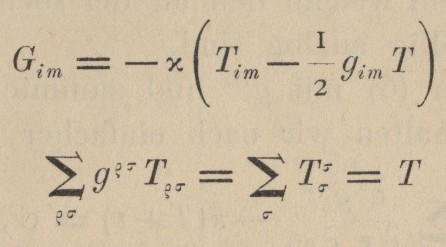
\includegraphics[scale=0.3]{fig/equation.jpeg}
    \caption*{\small 图:取自《引力的场方程》(\textit{Die Feldgleichungen der Gravitation})}
\end{figure}

\noindent Einstein 称之\textbf{广义相对论}(general relativity)。1919 年,Eddington 日全食实验验证了光线曲折的关键结论。彼时欧洲正值战后阴霾,故实验结果被相继刊登在各大报章的头版,冠之“科学革命”。这的确是现代物理学的伟大胜利。
\begin{figure}[ht]
    \centering
    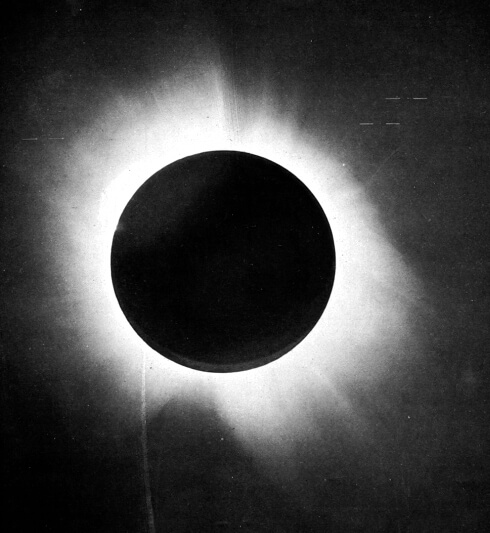
\includegraphics[scale=0.35]{fig/1919_eclipse_positive.jpg}
    \caption*{\small 图:Eddington 日全食实验结果}
\end{figure}
诚然,新符号自带神秘面纱,固然令人费解,败坏了大众印象。但我们不必妄自菲薄,无非是 Newton 理论需要微积分,而 Einstein 理论需要额外的几何学罢了。Einstein 方程仍类似于引力正比于物质的形式。它们都是人类漫漫长征的里程碑。所需的基本知识并非完全陌生,甚至一旦接受后,将发现 Einstein 的思想其实更自然、更简单。

想真正了解一套理论,仅仅知道方程还远不够。广义相对论与 20 世纪物理学所作的一些最蔚为奇观的预言相联系。读者多少在科普或艺术作品中,听说过这些现象:黑洞视界、平行宇宙、虫洞、宇宙膨胀、暗物质、信息熵、全息投影……1915 年时,这些还远未为人知,唯有人们理解方程的动力学后才能发现。花费的时间长得惊人,这其中的艰辛事迹并不逊色于 Einstein 的孤勇奋斗。本书聊物理时亦将对历史简要一瞥。目前,物理学能分析的一般解往往只是简单解的微扰,所谓的宇宙监督假设、一般条件的奇点等问题都未得到普适解答。这些问题恰恰是一套理论意义和适用范围的基础考量。我们只能期望后续理论,继续揭示出美丽的结构,帮助人类进一步认识世界。

谨以此段阐明本书之深度、广度。
本书以理工类专业一年级的多元微积分、线性代数、普通物理学为基础,致力讲述引力、时空等话题,为理解前沿进展作准备。将尽可能刨析概念动机,搭建同旧知识之桥梁。本书划分为广义相对论、数值计算以及量子理论,附录提供数学知识以飨读者。仅为证明单个命题所需的知识也放于附录,供有兴趣的读者查阅。细节未必完整提供,未提供时将给出简介和参考资料。故最终,附录在深度上似乎要讲透现代微分几何,但广度上又不完整。此乃笔者故意为之。因为本书不是要向读者大肆摆弄概念,而是补充看懂前沿所最少必要的、作了严格定义的数学。
本书看似未设习题,但实际上巧置省略,足当练习。
给出概念、结论时或通过字体改变暗示,或带编号地引入。不都采用编号只是为行文流畅,以免让本就不易的内容雪上加霜,但代价是失去链接便利。这固然重要,因为定义、命题在文中一般只出现一次,难免要来回翻阅,故敬请读者不厌其烦。

\begin{flushright}
\textit{夏草}\\
\textit{\the\year 年 \the\month 月}
\end{flushright}
\label{preface}       % 前言
    \chapter*{记号及单位制}
\addcontentsline{toc}{chapter}{\nameref{notation}} 

用分量指代物理量本身,书写将大大简化,且往往足以体现物理性质。比如,用 $E^i$ 可代表某个参考系所测电场 $\bm E=(E^1,E^2,E^3)=(E_x,E_y,E_z)$,用 $x^\mu$ 可代表四个时空坐标 $x^0=ct,x^1=x,x^2=y,x^3=z$。右上角的数字只是\textbf{指标}(index)而非乘幂。不必担心,很多情况下指标不会与乘幂相混淆。实在冲突时可根据上下文判断或额外注释。规定,时空指标一般取 $\mu,\nu$ 等希腊字母,遍及 $0,1,2,3$;空间指标取 $i,j$ 等拉丁字母,遍及 $1,2,3$。现代物理学总和指标打交道,初学者可能会感到复杂但又需要习惯。

物理学的代数运算常涉及对某指标的求和。注意到,单个因式中指标一般至多出现两次:出现两次的指标是求和哑元,称为\textbf{哑}(dummy)\textbf{标};留下的指标只出现一次,称\textbf{自由}(free)\textbf{指标}。比如,$4$ 维列向量 $X$ 的仿射变换可用方阵 $A$ 和常列向量 $Y$ 表为 $X'=AX+X_0$,分量表达为
\[X'^\mu=\sum_{\nu=0}^3 A^{\mu}{}_{\nu}X^\nu+ Y^\mu,\]
其中为了区分行列指标而将矩阵元的指标错开。在因式 $A^{\mu}{}_{\nu}X^\nu$ 中,$\mu$ 是自由指标,$\nu$ 是哑标。不与自由指标冲突的前提下,哑标可任意替换,比如换为 $A^{\mu}{}_{\sigma}X^\sigma$。多个因式之间可以出现重复哑标,因为它们是加法关系,比如用 $(A+B)$ 描述的线性变换:
\[X'^\mu=\sum_{\nu=0}^3 (A^{\mu}{}_{\nu}+B^{\mu}{}_{\nu})X^\nu=\sum_{\nu=0}^3 A^{\mu}{}_{\nu}X^\nu+\sum_{\nu=0}^3 B^{\mu}{}_{\nu}X^\nu.\]
$A^{\mu}{}_{\nu}X^\nu,B^{\mu}{}_{\nu}X^\nu$ 都出现 $\nu$。替换哑元后也可不重复,写作 $A^{\mu}{}_{\nu}X^\nu,B^{\mu}{}_{\sigma}X^\sigma$。单个因式可以出现多对哑标,比如,用 $\delta_{ij}$ 表示单位阵元,则 Descartes 系中线元的勾股定理是
\[\d\ell^2=\d x^2+\d y^2+\d z^2=\sum_{i,j=1}^3\delta_{ij}\d x^i\d x^j=\sum_{i=1}^3\sum_{j=1}^3\delta_{ij}\d x^i\d x^j,\]
当然,$\d x^2$ 的“2”表示平方而非指标。由乘法的交换、结合及分配律,求和顺序是无所谓的。
可以看到,\textbf{上标}(upper/raised indices)和\textbf{下标}(lower indices)位置总保持一致,这称为\textbf{指标平衡}。
如上性质说明,可省略求和号而只关心通项,毫不影响代数计算。由此 Einstein 提出\textbf{求和约定}:若某个指标一上一下成对出现,则要对该指标求和。也称对该指标\textbf{缩并}(contraction)。比如 $\d\ell^2=\delta_{ij}\d x^i\d x^j,X'^\mu=A^{\mu}{}_{\nu}X^\nu+ Y^\mu$。

物理学还涉及大量的坐标变换。将 4 维坐标系 $\{x\},\{x'\}$ 之间的光滑坐标变换记作
$x'^\mu=h^\mu(x^0,x^1,x^2,x^3)$,
通常混用符号地简写为 $x'^\mu=x'^\mu(x)$,链式法则给出
\[
    \d x'^\mu=\pdv{x'^\mu}{x^\nu}\d x^\nu,\quad \pdv{x'^\mu} =\pdv{x^\nu}{x'^\mu} \pdv{x^\nu}. 
\]
其中分母的上标看作分子的下标,$({\partial x'^\mu}/{\partial x^\nu})$ 就是分析学里的 \textbf{Jacobi 矩阵}。函数 $f$ 的全微分为
\[
    \d f=\pdv{f}{x^\mu}\d x^\mu=\del_\mu f\d x^\mu,
\]
因此梯度 $\del_\mu f$ 的变换是
\[
    \del'_\mu f=\pdv{f}{x'^\mu}=\pdv{x^\nu}{x'^\mu}\pdv{f}{x^\nu}=\pdv{x^\nu}{x'^\mu}\del_\nu f.
\]
注意对于 Jacobi 矩阵元,一般不用简记符 $\del_\mu$。

Jacobi 矩阵的互逆性:
\[\pdv{x^\mu}{\xi^\alpha}\pdv{\xi^\alpha}{x^\nu}=\pdv{\xi^\mu}{x^\kappa} \pdv{x^\kappa}{\xi^\nu}=\delta^\mu_\nu,\]
其中 $\delta^i_j$ 也是单位阵元。

部分量子场论教材选择统一使用下指标而只强调求和约定“总共重复两次”,更有甚者不区分指标顺序。这在讨论更深刻问题时出现缺陷,建议只在特殊情况采取简化。比如 $\delta^\mu_\nu$ 是考虑到 $I$ 是对称矩阵。

物理学是关乎实验测量的学科,讨论物理量的单位是极为重要的。在\textbf{国际制}(SI)中,我们认为时间、空间乃不同物理量,自然不会谈及“1s 等于多少 m”这种看似奇怪的问题。但在相对论中,这个问题很有意义,因为时空乃统一的概念。考虑令 $c=1$ 使 $x^0=t$,国际制下 $c$ 近似为 $3\times 10^8$ m/s,故这件事相当于
\[
1\,\mathrm s=3\times 10^8\,\mathrm m.
\]
这不会与国际制有任何冲突,因为在国际制中不会谈及“1s 等于多少 m”这种问题。这是国际制中一个可以利用的自由度。引力理论常涉及引力常量,把它们的数值都取为 1,即
\[
c=G=1,
\]
可简化大量公式的书写,这就是\textbf{几何单位制}(system of geometrized units),简称\textbf{几何制}(SG)。在国际制中 $G$ 近似等于 $6.67\times 10^{-11}\,\mathrm{m}^3/(\mathrm{s}^2\cdot\mathrm{kg})$,因此该操作相当于
\[
1\,\mathrm{kg}=\frac{6.67\times 10^{-11}}{(3\times 10^8)^2} \,\mathrm{m},
\]
可见这利用的是国际制的另一自由度。几何制便统一了长度、质量和时间的量纲。不涉及引力的量子理论经常使用如下的\textbf{自然单位制}(system of natural units),简称\textbf{自然制}(SN):
\[
c=\hbar=1,
\]
这里 $\hbar$ 在国际制中近似等于 $6.58\times 10^{-22}\,\mathrm{MeV}\cdot\mathrm s$。然而在计算物理量的数值时几何制就不再方便,因此我们要研究物理量、物理公式如何从几何制转换到其它单位制。一般来讲,所研究物理量在当前单位制是带上量纲的。比如,几何制下粒子物理常用 eV 作为质量单位,因为质能方程在几何制下统一了质量和能量量纲。欲将质量单位从几何制还原为国际制,无非是在问 eV 等于多少 kg。首先都转化到常用单位来,即
\[
1\,\mathrm{eV}=1.6 \times 10^{-19}\,\mathrm{C}\cdot\mathrm{V}=1.6\times 10^{-19}\,\mathrm{J}=1.6\times 10^{-19}\,\mathrm{kg}\cdot\frac{\mathrm{m}^2}{\mathrm{s}^2},
\]
代入几何制定义有
\[
1\,\mathrm{eV}=\frac{1.6\times 10^{-19}}{(3\times 10^8)^2}\,\mathrm{kg}.
\]
若所研究物理量在当前单位制只是一个无量纲数,则有可能它在其它单位制中有无量纲。比如定义直接告诉我们 $c$ 在几何制中无量纲。“真正无量纲”的量在任何单位制下都无量纲,因此不受单位转换的影响,如精细结构常数
\[
\alpha=\frac{e^2}{4\pi\epsilon_0\hbar c}=\frac{1}{137}.
\]
代入自然制定义得 $e^2/{4\pi\epsilon_0}=1/137$,这说明兼容自然制和精细结构常数的同时仍有自由度可利用。令
\[
c=\hbar=\epsilon_0=1,
\]
因而 $e=\sqrt{4\pi/137}$。由 $c=1/\sqrt{\epsilon_0\mu_0}$ 得 $\mu_0=1$。如上规定就称为 \textbf{Heaviside-Lorentz 单位制},简称 \textbf{HL 制}(SHL),其下不用再写出 Maxwell 方程中的常数。几何制和自然制还可共同构成 \textbf{Planck 制}(SP),这在量子引力理论中用得多。广义相对论常一齐使用几何制和 \textbf{Gauss 单位制},以便于引力和电磁学理论的书写:
\[
c=G=4\pi\epsilon_0=1,
\]
统称\textbf{几何 Gauss 制}。其中 $\epsilon_{0}$ 是真空介电常数(vacuum permittivity)。
进而根据光速 $c=1/\sqrt{\mu_0\epsilon_0}$ 可知真空磁导率(vacuum permeability)为 $\mu_{0}=4\pi$。 

当研究物理公式在不同单位制的转换时,最便捷的做法不是如上这样分析单位,而是分析量纲,即根据量纲补充缺失的常数。比如,在几何制下的 Schwarzschild 度规为
\[
    \d s^2=-\left(1-\frac{2M}{r}\right)\d t^2+\left(1-\frac{2M}{r}\right)^{-1}\d r^2+r^2\d\Omega^2,
\]
欲转换为国际制。注意几何制的定义是 $c=G=1$,使时间 $[T]$、长度 $[L]$、质量 $[M]$ 为相同量纲,这也是与国际制仅有的差距。我们只需在国际制下分析量纲,然后补上 $c,G$ 即可。$c$ 的国际制量纲为 $[T]^{-1}[L]$。$G$ 的国际制量纲为 $[T]^{-2}[L]^3[M]^{-1}$。研究系数 $g_{11}$,它在国际制无量纲。$\frac{M}{r}G^{\alpha}c^{\beta}$ 的量纲为 $[T]^{-2\alpha-\beta}[L]^{3\alpha+\beta-1}[M]^{1-\alpha}$。因此
\[
    -2\alpha-\beta=3\alpha+\beta-1=1-\alpha=0\implies \alpha=1,\beta=-2.
\]
$g_{00}$ 同理,故可得
\[
    \d s^2=-\left(1-\frac{2GM}{c^2 r}\right)c^2\d t^2+\left(1-\frac{2GM}{c^2 r}\right)^{-1}\d r^2+r^2\d\Omega^2.
\]
用相同方法可得到
\[
    R_{\mu\nu}-\frac 12 g_{\mu\nu} R=\frac{8\pi G}{c^4} T_{\mu\nu},\quad U^\mu U_\mu = - c^2,\quad \curl\bm B=\mu_0\epsilon_0\del_t\bm E+\mu_0\bm j, \quad \cdots
\]
方法皆完全相同。其中注意 $[\epsilon_0]=[T]^4[L]^{-3}[M]^{-1}[I]^2$($[I]$ 为电流量纲),而从几何 Gauss 制到国际制的过程是补充 $c,G,4\pi\epsilon_0$。再通常将 $c$ 去掉而引入 $\mu_0=1/c^2\epsilon_0$。

另外,有必要说明这样一种思想:有别于传统认知,物理公式应当视作“数”的公式而非“量”的公式。
简单来说,正如定义 $x^0=ct$ 一样,定义新单位制下某个物理量为旧单位制中的对应物理量乘以相应常数,这样物理方程中就再也不会出现该常数,因为它全部被收进了新定义里,比如,将 $G$ 收进场源质量里,并不影响其它任何物理量的计算;重新定义 $t'=ct$,其单位同距离单位彻底一致,时间和距离“共享”同一单位,因而 $c=1$ 是真正的“数”。不过从单位转换的角度看,这些数据并不需要收进任何一个物理量中,而是直接收进单位的相对关系里。
\label{notation}      % 记号及单位制

    %\setcounter{tocdepth}{3}   % 3-level 目录
    %\tableofcontents           % 目录

    \mainmatter

    %\part{经典理论}
    \chapter{经典引力场论}\label{chpt:GR}
\section{场论初步}
\subsection{时空}

物理学研究各类\textbf{事件}(event)。类似于记叙文,真实事件持续一段时间并占据一定体积,但可理想地只用时刻和空间点构成\textbf{时空点}来确定事件。目前认为物质都由\textbf{粒子}(particle)组成,其经典上占据一个空间点,日常物质隶属\textbf{有质粒子},我们只需一个有质粒子即可作为事件的\textbf{观者}(observer),实验上总选足够小的仪器。
尽管空间概念已深入人心,但它并不严格。我们不假思索地认为空间是同一时刻所有物质的分布,可实际上,观者只能对自己身上的事件做\textbf{直接观测}或\textbf{当时当地观测}(local measurement)。欲观测其它地方,单个观者必须想办法\textbf{间接观测}。这相当于处处设置观者形成\textbf{参考系}。任取事件,总存在一个观者经过它,进而记录直接测量结果,后续视需求再传递给其余观者。记录事件总选择坐标方法\footnote{读者或许认为可用叙述方法代替,即“此处何物发生何事”,而事件本身用其它自然语言叙述。但这只对其目击者有意义,缺乏科学数据的可传达性。若目击者欲转告事件发生的位置,或欲为后代留下记录,则不得不用经纬度这种明确、或某栋大楼正北一百米这种含蓄的坐标来描述位置。
叙述方法只对那些有真实事件的地方才有效,但\textit{大多数时空点是“空”的,从未发生真实事件}。
坐标空间是连续的不可数集,实际事件之集是离散的、有限归纳的集合,故二者不可能等同。},就涉及实数性测量。
我们就必须约定基准周期事件以定义时间单位、基准速率以获得长度单位,换言之,选取\textbf{标准钟}和\textbf{标准信号}。标准钟的读数称为\textbf{固有时}(proper time)。规定标准信号在任何时刻、任意参考系下,沿任意方向的\textbf{单程速率}相同,记作 $c$。
即使如此,标准钟也只确保各观者钟全同,即只约束\textbf{走时率}(rate),而对\textbf{初始设定}(setting)即零点选取未做要求。约定各零点才能得到坐标系,从而确定哪些事件构成时刻 $t$ 的\textbf{同时事件集} $\Sigma_t$,此即比空间更严格的替代概念。同时面在实验上的选取过程称为\textbf{对钟}或\textbf{钟同步}(clock synchronization),这更依赖于基准速率。

国际单位制用 $^{133}$Cs 原子钟(超精细跃迁周期)定义时间。2030 年计划改用光学原子钟的跃迁周期定义,候选者有 $^{87}$Sr 光学晶格钟、量子逻辑 $^{27}$Al$^+$ 离子钟等。
历史上对(双程)光速进行了高精度测量,且在任意 Newton 惯性参考系下测值相同,可认为光也是足够稳定的候选,进一步提升为\textbf{光速不变原理}。
国际单位制规定 $c=$ 299792458\,m/s,实际载体约定为真空电磁波或\textbf{光子}(photon)。
(静)质量特指粒子在相对静系所测质量,而光不存在相对静系,故光子没有甚至不可定义质量,属于\textbf{无质粒子}。

\begin{wrapfigure}{r}{.5\textwidth}
    \centering
    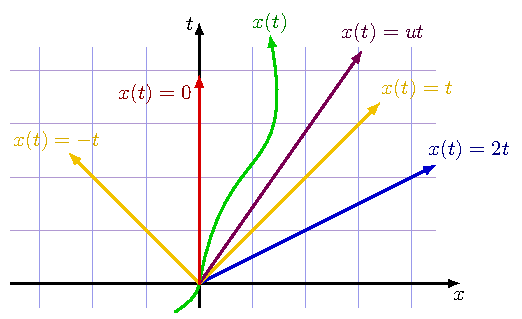
\includegraphics[width=.5\textwidth]{fig/chpt01/worldlines.pdf}
    \caption{\small 2 维时空图。以某惯性系为\textbf{绘图基准}是一种时空图的绘制习惯:将其坐标网格画成欧氏正交、时间轴未来方向朝上(空间轴右手排列)、尺度均匀的,这样迎合几何制,反向的光线也相互正交。}
\end{wrapfigure}

更普遍地,考察\textit{全体事件}规律排布的集合。比如,以某参考系为基准,可连续堆叠各时刻的同时事件集,即给空间补上时间轴就形成了\textbf{时空连续统}(spacetime continuum),简称\textbf{时空}。
故同时事件集又可形象地称为\textbf{同时面}(simultaneity surface)。
由于存在不同参考系选择,故建议直接默认存在一个 4 维\textbf{流形}(manifold)作为时空的理想模型。
流形就是点连续分布形成的集合,从而能建立坐标系\footnote{最初,我们仅用微积分和坐标系研究背景的\textbf{局部}(local)性质,建立了\textbf{微分几何}(differential geometry)。随着集合论和\textbf{拓扑学}发展,我们发现可将背景准确称为\textbf{拓扑空间}(topological space),其上提供了连续性定义。赋有坐标系的拓扑空间即流形,总规定系 $\{x\},\{x'\}$ 间的变换 $x'^\mu=x'^\mu(x)$ 可逆且光滑,这样可随意做微积分。
拓扑学提供了分析\textbf{整体}(global)性质的工具,便有了\textbf{现代微分几何}。}。
同时面只是截取时空的一系列切片。
实际上物理研究总要预设背景流形。比如,Newton 力学的研究背景是 $\R^3$ 空间;亦或更为抽象,如热力学会研究压强、温度的相图。
无论坐标系选取如何,描述任一事件的 4 个坐标依次记作 $x^0,x^1,x^2,x^3$,约定 $x^0$ 对应时间,正方向为\textbf{未来},反方向为\textbf{过去},其余坐标对应空间。比如选择 Descartes 系 $\{x,y,z\}$:
\eq{
x^0:=ct,\quad x^1:=x,\quad x^2:=y,\quad x^3:=z.
}
其中给时间乘上无歧义常数 $c$ 以使量纲一致。此后多采用几何制($c=G=1$),则 $x^0=t$,这样 $x^0,t$ 都可称\textbf{坐标时}。
时空中的曲线称\textbf{世界线}(worldline)。一族世界线构成\textbf{世界管}(worldtube)或\textbf{线汇}(congruence) $\mathscr C$。参考系 $\mathscr R$ 就是其每条世界线 $\gamma$ 都有观者对应的世界管。无交叉线汇 $\mathscr C$ 所占时空范围内每一点,都 $\exists! \alpha\in\mathscr C$ 对应。各观者按 $a^i$ 编号,且用固有时 $a^0$ 参数化,便建立了所谓\textbf{共动系}或\textbf{固有系} $\{a\}$。将实际对象从粒子改为流体质元,则观者即流线,进而对应于流体力学的 Lagrange 表述。凡示意时空及世界线的图就是\textbf{时空图}(spacetime diagram)。就一般的四维时空,固然画不出直观图像,但许多问题总能借助对称性,省略部分空间维度。

这些概念看起来都很显然,但事实远非如此:时空结构很可能极其怪异。
我们有野心将时空流形施以整个宇宙,但宇宙的拓扑形状迄今未知,也许在大尺度上无法用 $\R^4$ 覆盖;在 $10^{-15}$\,m 或 $10^{-25}$\,m 的小尺度上,不可能建立起足够刚性的参考系。目前我们认为这是因为微观量子性质,但也或许存在更深刻的物理。Wheeler 认为在 $10^{-35}$\,m 的亚核子尺度,量子引力的涨落极其剧烈,产生量子泡沫,戳破时空连续统。量子引力理论必须一致包含常数 $c,G,\hbar$,其中 $\hbar=h/2\pi$ 是约化 Planck 常数。简单分析可构造出具有长度量纲的\textbf{Planck 长度} $\sqrt{\hbar G/c^3}\approx 1.6\times10^{-35}$\,m,这意味着涨落的特征尺度在 Planck 长度的量级。
即便如此,人类仍只能间接地探测变态性质,即假设时空能用连续坐标描述。若基于这一假设成功描述了涨落,就有理由相信,至少日常生活中的时空结构良好,因为 Planck 长度确实太小。
对于复杂的拓扑,仍然希望邻域上能连续地标记坐标,用 $\R^4$ 去近似。这正是流形的定义。拓扑背景不提供物理量的计算能力。


\subsection{对钟与定域性}

如何对钟?
首先想到单程信号。人类总依靠观者和被观测物的信息交流来感知世界,比如能给予视觉图像的可见光,或天文观测。
无论可见光还是神经元生物电,其速率皆有限,传播过程花费时间,图像通常存在扭曲和滞后\footnote{对高速物体、强引力场现象的测算足以总结为一门课题,又同计算机图形学结合,称为\textbf{相对论视觉}。},
故不可能通过单程信号真正体会与周围的同时性。当然,这些信号依旧很快,以至于直到 Einstein 之前,人类都对同时性保有错觉。

\begin{figure}[ht]
    \centering
    \subfloat[\centering 静系对钟]{
    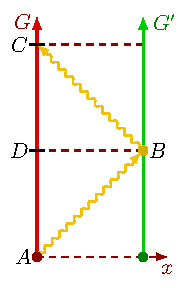
\includegraphics[height=.41\textwidth]{fig/chpt01/reflecting.pdf}
    }%
    \qquad
    \subfloat[\centering 动系对钟]{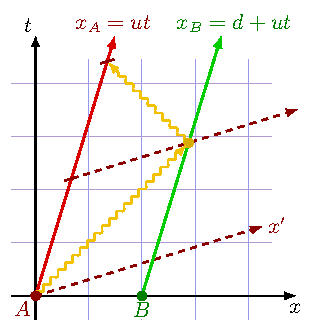
\includegraphics[height=.4\textwidth]{fig/chpt01/reflec2.pdf}
    }%
    \caption{\small 若以 $G$ 为绘图基准,只需使反射光与 $G$ 夹角呈 $45^\circ$ 即可使 $BD,AC$ 正交,结果如(a)。以该系为基准,研究一个运动惯性观者的对钟情况,结果如(b)。可见惯性系的坐标轴总关于 $45^\circ$ 斜线对称。}
    \label{fig:clock_syn}
\end{figure}

随后我们想到双程信号。
先讨论惯性参考系。
规定\textbf{惯性观者}走匀速直线。
无论技术发展如何,双程光速的测量原理至今仍和\textbf{Fizeau 程序}一致:从坐标原点发射球面光波,然后由放置在某处(尽量邻近)距离已知的镜子反射,随后记录光回到原点的时间,这样可计算光速。按现在的约定,不需要再测量光速,故以上步骤更倾向于测距。
任取某条惯性观者线 $G$,规定为坐标原点。设相对静止的另一惯性观者 $G'$;实验上若任意时刻测距均相同,就认为二者相对静止。二者可同属一个惯性参考系。
$G$ 在某时刻发出光(事件 $A$),到达 $G'$ 反射(事件 $B$),最后 $G$ 在某时刻接受该光(事件 $C$)。取 $A,C$ 的中间事件 $D$;实验上由标准钟测量。只需约定 $B,D$ 同时。
按此规定,惯性参考系的共动系称为\textbf{惯性坐标系}或\textbf{Lorentz 系}。不必认真区分时可笼统称为\textbf{惯性系}(inertial frame)。
总之,单程光速是约定的,不可实验测量(除非找到非光对钟法);我们可以测量的是双程光速,且用平均逼近瞬时。
且注意,并非所有参考系都能办到对钟。

\begin{figure}[t]
    \centering
    \subfloat[\centering $A,B$ 在 $S$ 中同时]{
    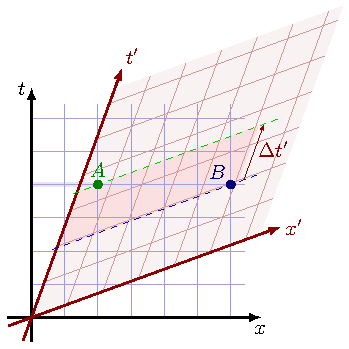
\includegraphics[width=.35\textwidth]{fig/chpt01/SIMULTANEITY.pdf}
    }%
    \quad
    \subfloat[\centering $A,B$ 在 $S'$ 中同时]{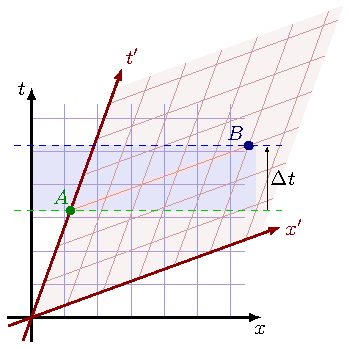
\includegraphics[width=.35\textwidth]{fig/chpt01/SIMU2.pdf}
    }
    \caption{\small 作某事件的同时面可投影得其坐标时。设静系 $S$ 和动系 $S'$。某事件的 $t$ 坐标可做 $S$系同时面截得,而 $t'$ 坐标可做$S'$系同时面截得。
    两个超新星的爆发事件在某系同时,但一般在另一系不同时。无法区别出特定的同时面,此即\textbf{同时的相对性}。}
    \label{fig:simurela}
\end{figure}

默认光速不变导致的遗憾是:有限能量下,亚光速有质粒子不能加速至光速。目前未发现超光速的快子(tachyon),故我们更愿意承认亚光速粒子、光子在时间上的连续性,即确认某两事件属同一粒子。凡信息就需载体,故光速是信息传速上限。注意,存在粒子能依次经历的两事件才称有\textbf{因果联系},可见并非所有事件都能涉及因果。
相互作用是一种信息,物质总通过动量、能量、质量的变化反馈。
可见相互作用至多以光速影响邻域,此即\textbf{定域性}(locality)或\textbf{局域性}。
从而,我们总能适当忽略环境对所关心的系统的作用以建立\textbf{孤立系统}模型,即忽略环境与系统的动量、能量、质量交换。此乃物理研究之根基:
宇宙是无所不包的最大时空,但我们往往只关心某些局部区域,即宇宙子系统。
理解子系统必须且可以使用孤立系统,否则讨论任何客体时都须考虑整个宇宙的作用,结果一事无成。
经典力学无定域性。Newton 引力定律是典型的超距案例,任二事件可通过 Newton 引力涉及因果。这一定律现只作为近似。对不具备连续性的事件亦能定义速率,比如介质光速。谈论超光速现象时往往指这种含义,以因果为前提的速度自然默认亚光速。

场提供了定域性最自然的图像,迄今所有基本相互作⽤都归结于定域场。两相距较远的粒子的相互作⽤解释为:粒子(作为\textbf{源})与场接触作用,再由场接触作用于另一粒子。接触作用强度均涉及粒子的\textbf{荷}(charge)。实际上,由于粒子动量、能量变化,为保持总和守恒,须设想粒子将其传递给周遭弥漫着的某种媒介。
起初我们这样理解场论:设想一种\textbf{试验粒子}(test particle),忽略其体积、形变及自旋,最重要地是忽略其自场对外场之干扰,就能测量受力来研究外场。每单位荷的场力即\textbf{场强}(strength),通常无关于试验粒子,往往又能表为某个\textbf{势}(potential)之导数。
在量子场论中,粒子解释为量子场的激发态。质子、电子、夸克等 Fermi 子携带作用荷,Bose 子场提供作用媒介。比如,电子场影响电磁场,产生波包(光子)传递电磁作用,在低能情形表现为电磁力。故严格来说,电磁场不依附于某个带电体,将总场分解为由各源所产生的部分是一种经典分析方法。

\subsection{相对论}

考虑任意惯性运动对象 $\gamma$ 于事件 $\gamma(\tau_1),\gamma(\tau_2)$ 经历的(elapsed along)固有时间 $\Delta\tau=\tau_2-\tau_1$。
惯性观者 $G$ 有办法直接测算这一时间吗?假设在 $G$ 系 $\{t,x,y,z\}$ 看来,$\Delta t$ 内 $\gamma$ 走过 $\Delta x,\Delta y,\Delta z$。Descartes 系的勾股定理为$\Delta\ell^2=\delta_{ij}\Delta x^i\Delta x^j$,其中 $(\delta_{ij})$ 为单位阵并对指标使用求和约定。$\delta_{ij}$ 称为\textbf{Kronecker 符号}。速率可写作 $u=\Delta\ell/\Delta t$。
总可设置与 $\gamma$ 相距 $L$、相对静止的镜子使光从 $\gamma(\tau_1)$ 发出并反射回 $\gamma(\tau_2)$,且镜面平行于运动方向。
由 $\gamma$ 系知 $2L=\Delta\tau$。
关键在于 $G$ 系中,镜面间距仍为 $L$,因为间距与运动方向垂直\footnote{测量长度即用量尺同时观察两端,涉及同时性。对任意沿垂线方向运动的尺 $A$,总可设置静止的尺 $B$ 使二者中垂线重合且静长相同。在 $B$ 看来,整个系统关于中垂线对称,故 $A$ 两端必同时到达 $B$ 所在直线,从而判断 $\sgn$($A$ 动长 - $B$ 静长),$\sgn$ 表示取符。这也等于 $\sgn$($A$ 静长 - $B$ 动长),因为在 $A$ 看来也有中垂线对称性,故这两个相遇事件在 $A$ 系也同时。但 $A$ 静长 = $B$ 静长,因此两个观者所处的情形是一致的,只是有反转或 $180^\circ$ 的对称。由相对性原理知 $\sgn$($A$ 动长 - $B$ 静长) = $\sgn$($B$ 动长 - $A$ 静长) = -$\sgn$($A$ 动长 - $B$ 静长),故 $A$ 动长 = $B$ 静长 = $A$ 静长。}。
由光速不变知 $2\sqrt{L^2+\Delta\ell^2/4}=\Delta t$,则 $\Delta\tau^2=\Delta t^2-\Delta\ell^2$,或者 $\Delta t=\gamma\Delta\tau$,其中 $\gamma:=1/\sqrt{1-u^2}\geqslant 1$ 是\textbf{Lorentz 因子}。可见 $\Delta t\geqslant\Delta\tau$,在观者看来,运动的时钟走时慢,这种现象称为\textbf{钟慢效应}或\textbf{时间膨胀}。这种效应是对称的,每个观者都认为其它的相对运动的时钟走时慢。
比如,宇宙射线含有介子,但其寿命非常短,即使以光速运动,穿透大气层所需时间也通常是寿命的几十倍。按理来说它不可能到达地面,但钟慢效应使其保持年轻,寿命“延长”,故仍可到达。

根据相对性原理,对任二惯性系 $\{x\},\{x'\}$ 必有两事件\textbf{间隔}(平方)$\Delta s^2:={\eta}_{\mu\nu}\Delta x^\mu\Delta x^\nu$ 的不变性,其中 $({\eta}_{\mu\nu}):=\diag(-1,1,1,1)$,即
\[-\Delta t^2+\Delta x^2+\Delta y^2+\Delta z^2=-\Delta t'^2+\Delta x'^2+\Delta y'^2+\Delta z'^2.\]
而 Newton 理论则分开定义绝对时间长度和空间长度。
$(\eta_{\mu\nu})$ 作为广义的单位阵,易证 $(\eta_{\mu\nu})=(\eta^{\mu\nu})$。
定义\textbf{号差}(signature)为 $(\eta_{\mu\nu})$ 的迹,本书一般选择 $+2$,称为\textbf{东海岸}习惯\footnote{量子场论教材常选择 $(\eta_{\mu\nu})=\diag(1,-1,-1,-1)$,号差为 $-2$ 即\textbf{西海岸}习惯。更有甚者选择将时间分量排在最后作为第 4 分量,这样有 $\diag(1,1,1,-1)$ 但并不影响号差。也有一种可能有哲学区别的习惯,称\textbf{Wick 技巧}:令 $x^0=\i ct$ 则线元还原回勾股定理 $\d s^2= \delta_{\mu\nu}\d x^\mu\d x^\nu$,伪转动变换的确变为 $x$-$\i ct$ 平面的旋转变换。除讨论某些理论复结构方面的问题外不使用这种做法。}。
该号差下,按 $\Delta s^2$ 为正、负或零,可分别称为\textbf{类空}(spacelike)、\textbf{类时}(timelike)或\textbf{类光}(lightlike)间隔。间隔不变性对类时间隔成立($\Delta\tau^2=-\Delta s^2$)。对类光间隔,注意光速不变与 $\Delta s^2=0$ 等价,仍成立。考察类空间隔。再次利用光测距,设置相对静止的镜子惯性运动,表示待测间隔。入射光的固有用时 $\Delta s$,出射光亦是 $\Delta s$。
外部观者看来,入射光用时 $\frac{L}{1-u}=\gamma\Delta s+\Delta t$,出射光用时 $\frac{L}{1+u}=\gamma\Delta s-\Delta t$。总共 $2\gamma\Delta s=\frac{L}{1-u}+\frac{L}{1+u}=2\gamma^2L$,则 $L=\Delta s/\gamma\leqslant\Delta s$。即运动方向上缩短 $1/\gamma$ 倍。这种现象称为\textbf{尺缩效应}或\textbf{长度收缩}。
蟹状星云和半人马星座 $\alpha$ 星之间的距离是相对的,不必诧异。
进而 $\Delta t=\gamma u\Delta s$。入射光总共走过 $\frac{L}{1-u}=\Delta\ell+\gamma u\Delta s$,则 $\Delta\ell = \gamma\Delta s$。故 $\Delta s^2=-\Delta t^2+\Delta\ell^2$,成立。

    \begin{figure}[t]
        \centering
        \subfloat[\centering 在 $S$ 中静止]{
        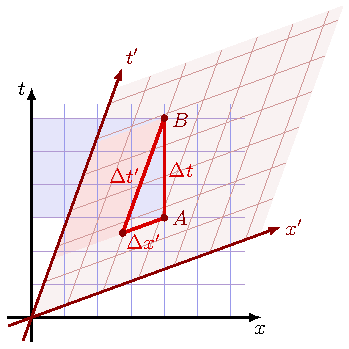
\includegraphics[width=.35\textwidth]{fig/chpt01/TIME DILATION S.pdf}
        }%
        \qquad
        \subfloat[\centering 在 $S'$ 中静止]{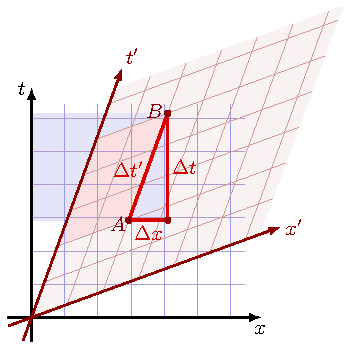
\includegraphics[width=.35\textwidth]{fig/chpt01/TIME DILATION S'.pdf}
        }
        \caption{钟慢效应}
    \end{figure}

考虑无穷小的事件间隔或\textbf{时空线元}
\eq{
\d s^2={\eta}_{\mu\nu}\d x^\mu\d x^\nu=-\d t^2+\d x^2+\d y^2+\d z^2.
}
设任意(分段光滑的)观者线 $C(\sigma)$,$\sigma$ 是任取参数,可有 $\gamma=\dv*{t}{\tau}$。考察它于事件 $C(\sigma_1),C(\sigma_2)$ 的固有时间 $\Delta\tau$。设置其固有坐标系 $\{x'\}$($x'^0=\tau$),$C$ 上事件总满足 $x'^i=0$,则 $\d\tau^2=-\d s^2$。它在惯性系 $\{x\}$ 下的参数式记 $x^\mu(\sigma)$,则
\eq{
\Delta\tau=\int_C \sqrt{-\eta_{\mu\nu}\d x^\mu\d x^\nu}=\int_{\sigma_1}^{\sigma_2}\sqrt{-\eta_{\mu\nu}\dv{x^\mu}{\sigma}\dv{x^\nu}{\sigma}}\d\sigma=\int_{\sigma_1}^{\sigma_2}\sqrt{-\eta_{\mu\nu}T^\mu T^\nu}\d\sigma,}
$T^\mu:=\dv*{x^\mu}{\sigma}$ 为关于 $\sigma$ 的\textbf{切矢}(tangent vector)在该系的分量,$\eta_{\mu\nu}T^\mu T^\nu$ 即模方。
切矢按模方符号(进而相应曲线)可类似分为三类。
\begin{figure}[t]
    \centering
    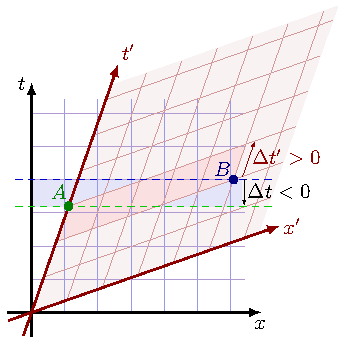
\includegraphics[width=.35\textwidth]{fig/chpt01/order.pdf}
    \caption{\small 若间隔类光或类时,则(由 $\Lambda^0{}_0>0$ 联系)各惯性系将一致认同两个事件的先后顺序。但对于类空间隔,其事件的坐标时差距可以在不同惯性系下取任意实数。不同观者对其先后次序各抒己见。
    类空间隔的事件没有因果联系。}
    \label{fig:spacelike}
\end{figure}
类时或类光线统称\textbf{因果线}(causal curve),能用因果线连接的事件正是具有因果联系的事件。在 $\R^4$ 中这等价于用非类空间隔连接。
类光矢量亦称\textbf{零模}(null)矢量,构成的集合 $C_N$ 称\textbf{光锥}(light cone)。
$\Delta\tau$ 即观者线的线长,故 $\tau$ 又称\textbf{线长参数}。$\lambda=a\tau+b$ 统称\textbf{仿射参数}(affine parameter)。
光对其世界线上的事件标记为一致坐标时,即对光而言不能定义固有时。光不能充当观者。描述光线可用坐标时 $t$ 参数化。

设 $V^\mu$ 类时,$W^\nu$ 是非零类时或类光矢量,则由三维 Cauchy 不等式知 $V^\mu W_\mu<0\eqto V^{0} W^{0}>0$,即 $V^\mu,W^\nu$ 具有相同的\textbf{时间指向}。
因此可在光锥及其内部定义等价关系。约定某一惯性系后,规定 $V^0>0$ 是\textbf{指向未来}(future directed)矢量,那 $V^0<0$ 是\textbf{指向过去}(past directed)矢量。光锥被分为了\textbf{未来光锥}和\textbf{过去光锥}。讨论时间的反演时可以考虑指向过去的惯性系。类空矢量无未来或过去之分。

\begin{figure}[t]
    \centering
    \subfloat[\centering 3 维时空的光锥]{
     \begin{tikzpicture}[scale=1.5]
    \draw (-1,-1)--(1,1);
    \draw (-1,1)--(1,-1) node[right]{$\scriptstyle C_N$};
    \draw[->] (0,0)--(0.8,0.8) node[below right]{\scriptsize 类光矢量};
    \draw[->] (0,0)--(-0.9,-0.3) node[above left]{\scriptsize 类空矢量};
    \draw[dashed] (0,0)--(-0.175,0.175/0.2);
    \draw[->] (-0.175,0.175/0.2)--(-0.25,0.25/0.2) node[above left]{\scriptsize 类时矢量};
    \draw (0,1)  ellipse [x radius=1, y radius=0.13];
    \draw[dashed] (1,-1) arc [start angle=0, end angle=180, x radius=1, y radius=0.13];
    \draw (1,-1) arc [start angle=0, end angle=-180, x radius=1, y radius=0.13];
    \end{tikzpicture}
    }%
    \quad
    \subfloat[\centering 因果结构]{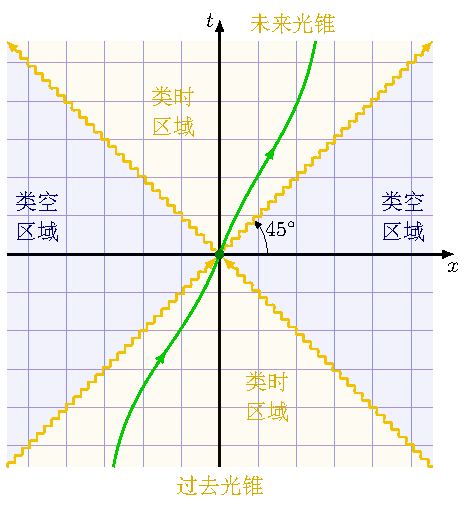
\includegraphics[width=.3\textwidth]{fig/chpt01/structure cone.pdf}
    }
    \caption{光锥}
\end{figure}

惯性系 $\{x\},\{x'\}$ 间满足
\eq{\eta_{\alpha\beta}\d x'^\alpha\d x'^\beta=\eta_{\gamma\sigma}\d x^\gamma\d x^\sigma\iff \eta_{\alpha\beta}\pdv{x'^\alpha}{x^\gamma}\pdv{x'^\beta}{x^\sigma}=\eta_{\gamma\sigma},}
由 \eqref{eq:chris} 式可快速证明变换的仿射性:
\eq{\label{Lorentz} 
\pdv{x'^\alpha}{x^{\gamma}}{x^\epsilon}=0\iff  x'^\mu=x_0^\mu+ \Lambda^{\mu}{}_{\nu}x^\nu,\quad \text{$\Lambda^{\mu}{}_{\nu}$ 满足 $\eta_{\mu\nu}\Lambda^{\mu}{}_{\sigma}{\Lambda^{\nu}}_{\lambda}={\eta}_{\sigma\lambda}$}.
}
满足上式的变换称\textbf{Poincaré 变换}。
置 $S,S'$ 的时空原点重合,则 $x^\mu_0=0$,变换仅线性。设空间轴初态重合,但 $S'$ 相对于 $S$ 沿共同 $x,x'$ 轴匀速运动,则 $y,z$ 坐标一致。设正方向速率 $u$,则 $x=ut$ 对应 $x'=0$。    
进而得到(或直接利用钟慢、尺缩)\textbf{二维 boost 变换}:
\eq{
     t'=\gamma( t-u x),\quad x'=\gamma( x-u t).
}
普通教材称之 Lorentz 变换。Einstein 最初用同时性对钟定义、仿射性假设得到上式,而线元后来才由 Minkowski(参见 \cite{PrincipleR})提出。
由此发展出来的理论由 Lorentz 命名为\textbf{相对性理论}(the theory of relativity),简称\textbf{相对论}。当下主流称呼是\textbf{狭义相对论}(special relativity)。boost 变换仅为特例,一般情形的推导见 \ref{sec:PoincareLorentz} 节。
因为上式在低速极限下退回 Galileo 变换 $t'=t,x'=x-ut$,从而兼容经典力学。
“boost”取时间轴上的推动之意,但由图 \ref{fig:boost} 可知,一个较好称呼是\textbf{伪转动}(pseudo rotation)。

数学上给定 $\d s^2=g_{\mu\nu}\d x^\mu\d x^\nu$ 后用积分定义线长、矢量模,借圆弧和三角函数定义角,最后按投影定义切矢的内积(inner product),等价于 $g_{\mu\nu}V^\mu W^\nu$。可用该式定义内积,反之给出线长和夹角,此即线性代数教材的逻辑。$g_{\mu\nu}$ 乃人为给定,称为\textbf{度规}(metric)。据此定义有 $g_{\mu\nu}=g_{\nu\mu}$。取 Descartes 系,代入勾股定理 $\d\l^2=\delta_{ij}\d x^i\d x^j$ 就得欧氏几何,$\delta_{ij}$ 称\textbf{欧氏度规}。
欧氏几何现降级为一种选择,而非保守派所认为的绝对真理。比如 ${\eta}_{\mu\nu}$ 就是\textbf{闵氏度规},对应\textbf{闵氏几何};还可有双曲几何 $\d\l^2=(\d x^2+\d y^2)/(1-x^2-y^2)$,当接近 $x^2+y^2<1$ 边缘时,该线元相较于欧氏线元会越来越大,但它除平面几何第五公理外符合其余公理。公理的特征是可替代性,故这说明第五公理不能由其余公理推出,而只能作为欧氏几何的约束。
第 $\alpha$ 坐标轴可按相应 $x^\alpha$ 参数化,切矢 $\dv{x^\mu}{x^\alpha}=\delta^\mu_\alpha$ 称为\textbf{坐标基矢},这里 $\delta^\mu_\nu$ 也是 Kronecker 符号。$\{\delta_\alpha^\mu\}_{\alpha=0}^3$ 称为坐标系的\textbf{坐标基}。可见惯性系的时空轴正交,因为 $\eta_{\mu\nu}\delta^\mu_0\delta^\nu_i=\eta_{0i}=0$。这说明我们进行对钟并发展相应的几何后,同时面与各观者线正交,换言之,时空正交性在实验上由对钟产生\footnote{理论上的几何概念只能代数地定义,如勾股定理。实际用物理定律来约定一类基准,各类规则形状的日常用品就是这样生产的。比如,默认光走直线、Lorentz 力确定空间正交性、宇称不守恒确定右手性。}。
虽然时空图中动系坐标轴不是欧氏正交,但被约定为时空上的正交。

\begin{figure}[p]
    \centering
    \subfloat[\centering 空间转动变换]{
    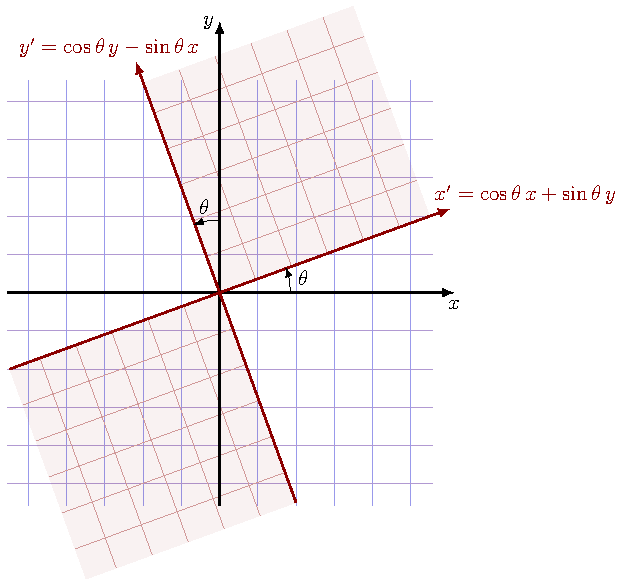
\includegraphics[width=.45\textwidth]{fig/chpt01/ROTATION.pdf}
    }%
    \subfloat[\centering 时空伪转动变换]{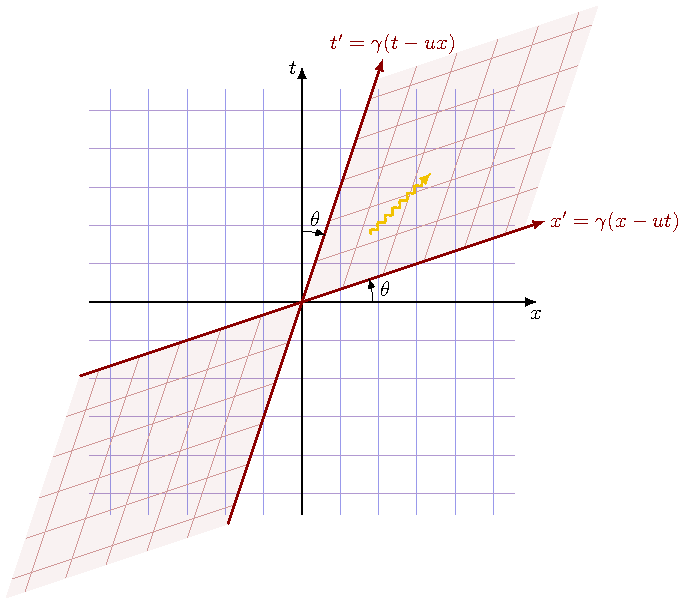
\includegraphics[width=.49\textwidth]{fig/chpt01/boost.pdf}
    }

    \subfloat[\centering 负方向伪转动]{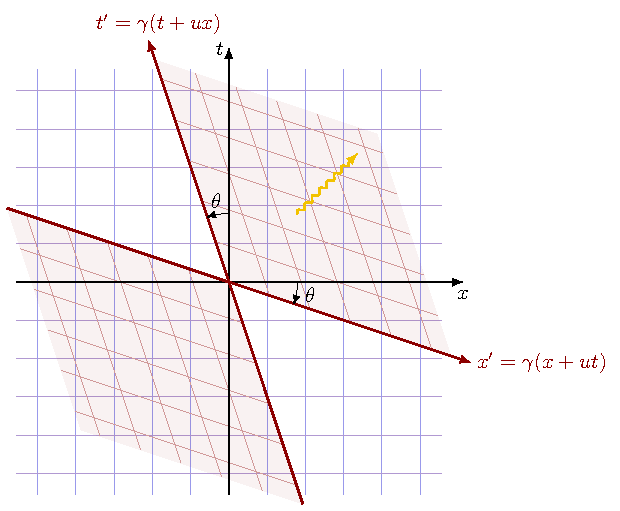
\includegraphics[width=.44\textwidth]{fig/chpt01/INVERSE BOOST.pdf}
    }
    \subfloat[\centering Galileo 变换]{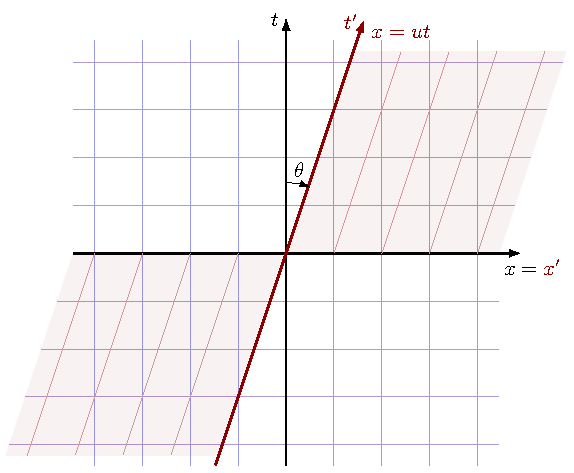
\includegraphics[width=.42\textwidth]{fig/chpt01/GALILEAN.pdf}
    }
    \caption{\small
    $x'$ 轴直线 $t'=0$ 即 $t=u x$,同理 $t'$ 轴即 $t=(1 / u) x$。速率 $u$ 代表动系时间轴斜率。以转动变换类比之,相应的三角函数应替换为双曲函数。$\theta:=\operatorname{artanh}u$不是绘图意义的倾角,称为\textbf{快度}。这样 $\cosh\theta=\gamma,  \sinh\theta=\gamma u$,变换为 $t'= t\cosh\theta - x\sinh\theta, x'= x\cosh\theta -t \sinh\theta$。
    如图,光速相对于日常情形较大,因此图上光线应“下压”,则空间轴转动不明显,退回 Galileo 变换,大家共用绝对时间。快度概念比速度更简洁。比如,设 $u_1=\tanh\theta_{1}$ 是 $B$ 相对于 $A$ 的速度,而 $u_2=\tanh\theta_{2}$ 是 $C$ 相对于 $B$ 的速度,可证 $C$ 相对于 $A$ 的速度是 $u={(u_{1}+u_{2})}/{(1+u_{1} u_{2})}=\tanh(\theta_1+\theta_{2})$,此即速度叠加公式。
    }\label{fig:boost}
\end{figure}

总之,闵氏几何必须依赖于前文叙述的光速不变、相对性原理,以及一些额外条件,如光走直线、不存在其它不变常数、时空均匀性等。通过修改这些条件得到的新理论,可以用于实验检验,结果显示与相对论相差不大。
并且,相对论以及在此基础上发展的量子场论的许多结果,都在极高精度上获得验证。我们目前有充分理由认可闵氏,直至存在实验明显证否。

\newpage
\begin{figure}[!h]
    \centering
        \subfloat[\centering 双曲线校准]{
        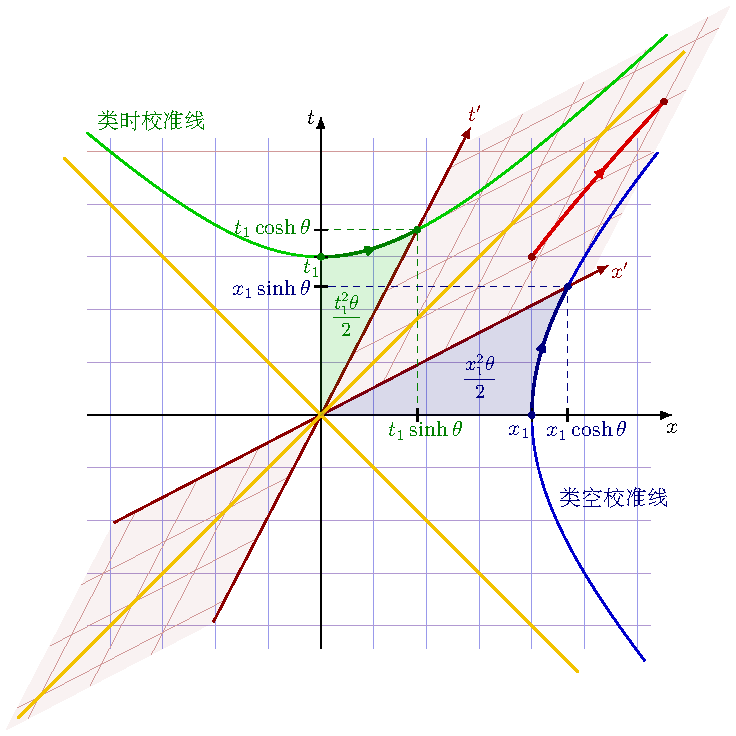
\includegraphics[height=.45\textwidth]{fig/chpt01/HYPERBOLOIDS.pdf}
        }
        \subfloat[\centering 钟慢效应]{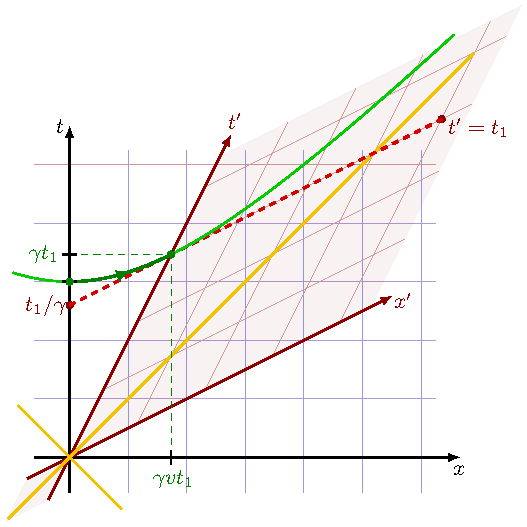
\includegraphics[height=.45\textwidth]{fig/chpt01/INVARIANT HYPERBOLOIDS.pdf}
        }
    \caption{\small 比较间隔的方法是用双曲线校准。令双曲线 $x^2-t^2=x_1^2$,其与 $x$ 轴交于 $\left(t,x\right)=(0,x_1)$。双曲线上的点 $(t,x)=(x_1\sinh\theta, x_1\cosh\theta)$ 与原点连线是类空间隔且恒定,可用来比较类空间隔,故称\textbf{类空校准线}。从 $(0,x_1)$ 至 $(t,x)$ 扫过角度 $\theta$,易得扫过面积为 $x_1^2\theta/2$,可类比欧氏几何的圆。同理推知\textbf{类时校准线}的结论。
    例如,两个观者都看到 $S$ 系原点上的时钟读数“0”,但直线 $t'=t_1$ 与该时钟世界线($t$ 轴)在 $\left(t,x\right)=(t_1,0)$ 下方的 $(t_1/\gamma,0)$ 相交。故$S'$ 系的钟根据同时面 $t'=t_1,t'=0$ 认为 $S$ 的钟慢。}
\end{figure}
    \begin{figure}[!h]
        \centering
        \subfloat[\centering 在 $S'$ 中静止]{
        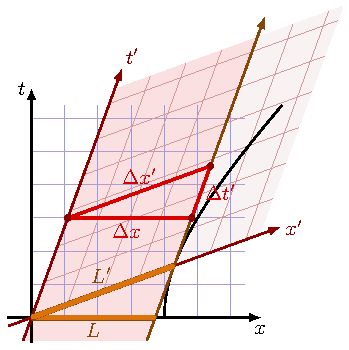
\includegraphics[height=.45\textwidth]{fig/chpt01/INVARIANT 2.pdf}
        }
        \qquad
        \subfloat[\centering 在 $S$ 中静止]{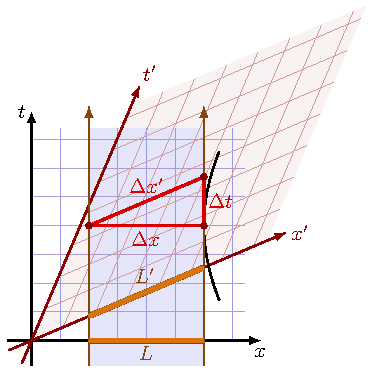
\includegraphics[height=.45\textwidth]{fig/chpt01/INVARIANT 1.pdf}
        }
        \caption{\small 尺缩效应}
    \end{figure}

\newpage
\begin{wrapfigure}{l}{.45\textwidth}
    \centering
    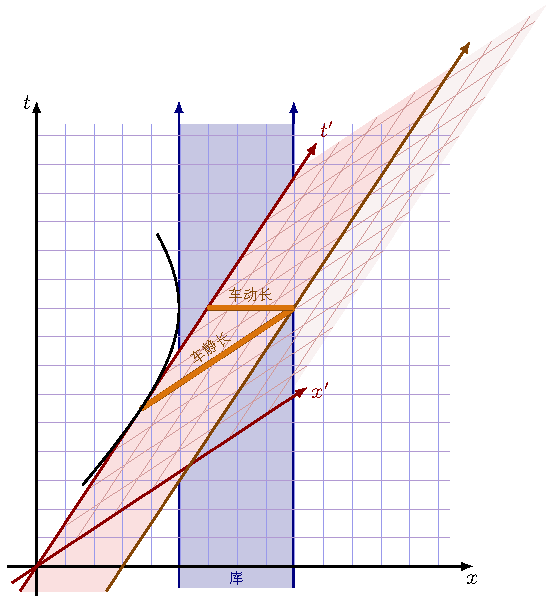
\includegraphics[width=.45\textwidth]{fig/chpt01/ladder.pdf}
    \caption{汽车匀速进库}
\end{wrapfigure}
    
    尺缩效应还导致\textbf{车库佯谬}\footnote{Ladder paradox,由 Rindler 提出,最初借梯子和谷仓(barn)举例,还可用火车和隧道。}。
    设汽车与车库静长相等。汽车朝库匀速前进,司机认为动库变短、不能放下,司库认为动车收缩、放下有余。二者矛盾吗?不妨设车库无后墙(类似于隧道洞口),画图时借用校准曲线以保证车和库有相等静长。由图易见,以司库所在惯性系的同时面衡量,车短于库;以司机所在惯性系的同时面衡量,车长于库。两人观点都对,因为同时性的相对性导致结论的相对性。“\textit{到底}放下还是放不下?”这种问题没有意义,正如在尺缩问题中“到底哪把尺子较长”亦无意义。我们若真要“比较”,能让各位意见一致的做法只能是都放入静系中去。
    从因果角度来理解将更便于在脑海里建立物理图像。“车尾接触入口”“车头接触出口”两个事件没有因果联系,故二人观点都对。我们在脑海中,不假思索地以为有因果联系,这个错觉来源于火车的车身。但在相对论中没有严格的刚体,只能将车身各质元的恒定高速运动理解为独自的、互相影响很小的。当然,现实生活中没有这么长且如此高速的火车,相互作用能在车头车尾间迅速传递,的确具有因果联系。
    当车库有坚硬后墙时,车头固然撞墙停止。但撞墙信息以相互作用纵波传至车身各部分皆需时间,只当车尾获悉后整个车身才能停住,因而汽车将缩至比司库期初所测
    
    \begin{wrapfigure}{r}{.35\textwidth}
        \centering
        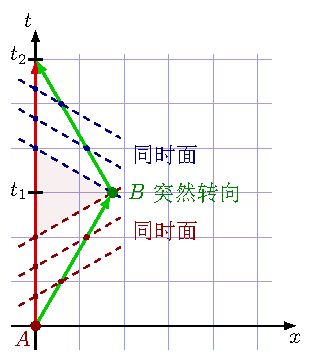
\includegraphics[width=.35\textwidth]{fig/chpt01/TWIN PARADOX.pdf}
        \caption{孪生佯谬}
        \label{fig:twin}
    \end{wrapfigure}

    \noindent 长度更短的程度。这时的确在谁看来都装得下。设材料性质理想,使信息传递为光速且质点获悉信号后立即停止,读者不妨在图上补出撞车后的时空图。

    最后,著名的\textbf{孪生佯谬}(twin paradox)就是说,设一对双胞胎从某时空点分离,并回合于另一时空点,则惯性运动者将年长于非惯性运动者。
    前文已直接证明了这一点。图 \ref{fig:twin} 给出了三角情形,也可理解为,折线的同时面在 $B$ 处发生突变,因此惯性观者多出了图中阴影部分的时间差。
    结论是不能交换的,因为不能将相对性原理滥用于非惯性系和惯性系间;而实际情形中,两人非质点,因此走惯性运动较为舒适,而走非惯性运动将感受到巨大的加速度,使相对论现象足够明显的物理量达光速级。



    
\subsection{惯性系存在性}

前文对惯性系存在性的考虑,仍然承袭 Newton 体系的思维,即认为存在一个绝对静止系,则相对其匀速的物体可作为惯性系,而具有加速度的物体不能充当惯性系。然而,并无任何先验原理帮助我们确定绝对静止系在哪。
实际上,物质间皆存在引力,且可在长程上传递,这称为引力的\textbf{万有性},而理想惯性系必须远离所有物质以孤立,因此严格来说不存在。但实验上 Newton 定律一定程度适用于地面系,可见惯性系仍是有用概念。问题出在哪里?

物质在仅受引力作用时有\textbf{Galileo 性}:任意试验质点在同一时空点所受加速度相同(由任意坐标系测量),与内部结构及组成无关。Newton 对 Galileo 性的解释如下。$\bm f=m_I\ddot{\bm x}$ 定义的质量 $m_I$ 是\textbf{惯性质量}。Mach 提出了一种测量性定义:承认动量守恒并规定好某一物体的质量数值,使二者产生相互作用(如碰撞),根据加速度比值便可测得另一物体的质量。而 $\bm f=m_G\bm g $ 定义的质量 $m_G$ 是\textbf{引力质量}或\textbf{引力荷}。联立有 $\ddot{\bm x}=(m_G/m_I)\bm g $,说明 Galileo 性即指比例 $m_G/m_I$ 与物质本身无关,重新定义 $G,m_G$ 还可使此二概念不再区分:$m_I=m_G\Rightarrow\bm g =\ddot{\bm x}$。
设 $A,B$ 共同自由落体,二者相对加速度近似为零。关键在于,\textit{总能以一者为研究对象,另一者抽象为背景坐标系}。比如,$B$ 可以是一部足够小、无自转的封闭电梯,而 $A$ 是乘客,则 $A$ 将感到失重。Newton 理论指出 $B$ 系中出现惯性力,但它与引力局域抵消,$B$ 系中做任何局域的力学实验结果都与惯性系等效,尤其在抛弃绝对系概念后,我们无法分辨。

对任意自由落体质点而言,总存在局域坐标系,使质点相对于该系的动力学,像是在理想惯性系中一样。这种坐标系称为相应质点的\textbf{局域惯性系}。参考系的惯性性在局域上不可物理观测,惯性系可以且只能局域建立。任何我们所规定的惯性系,其实均是局域惯性系。Newton 的绝对运动不是相对于绝对系的运动,而是相对于局域惯性系的运动。
Einstein 于 1907 年察觉到这一等效性\footnote{顺便提一句,Newton 是知道这件事的:“\textit{无论诸物体彼此间以何种方式运动,若它们被沿着平行线的相等加速力所推动,则它们都将继续彼此间的运动,遵循的方式就如同没有那些力作用一样}。”——《原理》\cite{Principia} 推论 VI “运动定律”。可用这个推论来计算太阳系中月球的复杂运动。在地球系下,惯性力和太阳引力在良好近似下相互抵消,那么月球就遵循一个 Kepler 轨道。}。
尽管 Galileo 性是谈及质点的,但他坚信任何物质都应如此,他称之为\textbf{等效原理}(equivalence principle)。这里要包括电磁、量子等任何实验:容易想象,在落体电梯里打开手电筒,光相对电梯按一定频率走直线,而在地球上看光线只能弯曲且频率变化,便能预言光的偏折、红移。

现在再研究可多大程度上建立局域惯性系。对于两相距足够远的时空点,引力加速度一般不同。一水球各部分受力不均,从而出现形变。这就是\textbf{潮汐效应}。邻近质元间相对力也称\textbf{潮汐力}(tidal force),相对加速度称\textbf{潮汐加速度}。可见,理想的局域惯性系只建立在自由落体质点的世界线上。当然,只要在设备精度内未观测到潮汐,就可认为是实验意义的局域惯性系。若物质集团的尺度较大,密度较稀疏,则外部引力较弱,潮汐现象不明显,因此能近似为局域惯性系的时空区域很大。比如,地球、太阳系、银河系能作为局域惯性系的范围应依次增大。现在,理想惯性系只视作局域惯性系在无引力时延伸的极限。综上,实验意义的局域惯性系的范围由外部引力强弱决定。

\subsection{广义协变性}

物理学用矩阵书写物理量,如标量、矢量;Cauchy 研究弹性力学时还意识到,一点处质元与质元的作用力不能只由一个数组描述,需用多维矩阵,称之为\textbf{张量}(tensor)。
物理量总与其分量联系,因为观者只能利用仪器的坐标系测量分量,提取实验数据。
关键就在于坐标变换下物理量的分量如何变。
分量及其方程的数学形式在某类坐标变换下不变,称为\textbf{协变性}(covariance)。狭义相对论具有 Lorentz 系间变换下的\textbf{Lorentz 协变性}。
现在就可更严格地阐述狭义相对论的原理:\textit{物理方程具有 Lorentz 协变性,且与物质状态无关的标量常数保持同样的值},如 $c=1,\pi/2$ 和 $\hbar$。合称\textbf{Lorentz 不变性}(invariance)。
例如,经典电动力学虽然能将光解释为无源电磁波,但 Maxwell 方程的 Lorentz 协变性只涉及其数学形式,将协变性提升为不变性才能给出光速不变。

等效原理指出惯性系与非惯性系局域难以区分,因而最好是认同任意参考系,即一种广义相对性原理。更进一步地,我们本就默认物理对象、规律不受坐标系影响,即\textbf{坐标冗余性},因而不仅考虑与参考系有关的那类坐标系,任意坐标系均可接受,即直接寻求对任意坐标变换的\textbf{广义协变性}。
由前文知曲线线长可由切矢的积分给出。
广义协变性要求同一切矢在任意坐标系下皆表以 $T^\mu=\d x^\mu/\d\sigma$ 形式,则根据全微分知:
\eq{
    T'^\mu= \pdv{x'^\mu}{x^\nu}T^\nu.
}
称这种变换为\textbf{逆变的}(contravariant),按这种方式变换的矢量称为\textbf{逆变矢量}(contravector)或切矢,故上指标又称\textbf{逆变指标}。一点处全体逆变矢量构成该点\textbf{切空间}(tangent space)。实际上,物理学很多矢量都与相切有关,因而是逆变矢量。可以存在变换与之互逆的矢量:
\eq{\omega'_i=\pdv{x^j}{x'^i}  \omega_j,}
则称\textbf{协变矢量}(covector)或\textbf{余切矢}(cotangent vector),简称\textbf{余矢}。下指标称\textbf{协变指标}。这一称呼与“协变性”有区别,没有物理方程“逆变性”的说法。

度规的定义实际默认了\textbf{Gauss 假设}:希望存在坐标系使线元表为勾股定理。进而在广义协变性要求下保持二次型:
\eq{
    g_{\mu\nu}\d x^\mu\d x^\nu=g'_{\gamma\sigma}\d x'^\gamma\d x'^\sigma\iff g'_{\gamma\sigma}= g_{\mu\nu}\pdv{x^\mu}{x'^\gamma}\pdv{x^\nu}{x'^\sigma}.
}
主流几何理论总研究二次型,不研究 $\d\l=(|\d x|^3+|\d y|^3)^{1/3}$ 等。上式是合同变换,$g_{\mu\nu}$ 保持可逆,故总可定义 $(g^{\mu\nu}):=(g_{\mu\nu})^{-1}$,即满足 $g^{\mu \lambda} g_{\lambda\nu}=g_{\nu\lambda}g^{\lambda\mu}=\delta^\mu_\nu$。称 $g^{\mu\nu}$ 为\textbf{度规逆}。
规定 $T_\mu$ 相应的\textbf{对偶矢量}(dual vector)为 $T_\mu:=g_{\mu\nu}T^\nu$,内积就可紧凑写作 $V^\mu W_\mu=V_\mu W^\mu$。它为协变矢量一例。也可对偶回去:$T^\mu=g^{\mu\nu}T_\nu$。

推而广之的概念称为\textbf{广义协变张量},本书简称张量。当然,称 $T^{\cdots}{}_{\cdots}$ 是张量,准确是想称分量等价类 $[T^{\cdots}{}_{\cdots}]=\{T^{\cdots}{}_{\cdots},T'^{\cdots}{}_{\cdots},\cdots\}$ 是张量。
$(k,l)$\textbf{型张量}简称 $(k,l)$-\textbf{张量},应满足如下\textbf{张量变换律}:
\eq{
    T'^{\mu_1\cdots\mu_k}{}_{\nu_1\cdots\nu_l}=T^{\rho_1\cdots\rho_k}{}_{\sigma_1\cdots\sigma_l}\pdv{x'^{\mu_1}}{x^{\rho_1}}\cdots\pdv{x'^{\mu_k}}{x^{\rho_k}}\pdv{x^{\sigma_1}}{x'^{\nu_1}}\cdots\pdv{x^{\sigma_l}}{x'^{\nu_l}},
}
可记忆为是满足指标平衡的 Jacobi 矩阵元乘积,这样就可快速写出公式。
常习惯于先将上指标写完,再错开地写下指标。
只要求 Lorentz 协变性 $\pdv*{x'^\mu}{x^\nu}=\Lambda^\mu{}_\nu$ 则称\textbf{Lorentz 张量}。张量一定是 Lorentz 张量,反之不然。
$(k+l)$ 叫作张量的\textbf{阶}(rank)。$(0,0)$-张量就是不变标量。$(n,0),(0,n)$ 型分别称\textbf{$n$ 阶逆变、协变张量}或 $n$-张量,比如切矢是 1-逆变张量,余矢是 1-协变张量;度规是对称、非退化的 2-协变张量;Kronecker 符号是 2-张量。由张量的变换律,若存在坐标系使其分量为零,其在任何坐标系下分量都为零,故不论何型都称\textbf{零张量}。
基本运算性质如下:
\begin{enumerate}
    \item 张量的直接拼凑称\textbf{张量积}\footnote{电动力学、量子力学中的\textbf{并矢}(dyadic)就是张量积,如 $\bm A\bm B,|\psi\rangle\langle\phi|$ 等。},结果仍为张量,比如将 $T^\mu,S_{\lambda\sigma}$ 拼成 $T^\mu S_{\lambda\sigma}$,变换式无非将各自 Jacobi 矩阵元按实数规律相乘;
    \item 张量缩并仍是张量,因为变换式只是消去一对 Jacobi 矩阵元;
    \item 若干张量线性相加仍是张量;\item 指标升降约定用 $g_{\mu\nu},g^{\mu\nu}$,构成\textbf{度规对偶};
    \item 求坐标偏导:$T^{\cdots}{}_{\cdots,\mu}=\del_\mu T^{\cdots}{}_{\cdots}=\pdv*{T^{\cdots}{}_{\cdots}}{x^\mu}$,但保持张量性的导数见 \ref{sec:co-di} 节。
\end{enumerate}

虽然这在物理和计算上没有问题,但似乎还是缺了些什么。我们期望的是如果有分量,就应该有某种数学对象,使得分量是这一数学对象在不同坐标系下的不同转述。当然希望能用类似 $A=A^I e_I$ 的形式表述矢量。换一组 $\{e_I\}$ 就可给出另一组分量,但这又涉及 $e_I$ 的定义是什么。鉴于对切矢图像的充分观察,Cartan 率先给出了这一数学对象的构造,称为\textbf{映射语言},详见附录 \ref{appx:manifold}。但这套框架比较抽象。很多人因其语言之优雅,成了 Cartan 及其后世之信徒,常声称其优势在于“无需借助坐标”,即 Cartan 关于矢量的定义是“几何”的、“坐标无关”的。这一论断当然过分夸张。
这种所谓“坐标无关”,我们给出准确陈述:\textbf{坐标独立性}(coordinate independence)或\textbf{坐标选择无关},从而支撑了物理上的坐标冗余性。
最重要地,计算时还存在一类高维矩阵不满足任何协变性,常称\textbf{赝张量}。
对于赝张量,映射语言需要将其强行定义为“坐标系依赖的张量”,非常累赘,分量语言反成聪明的选择。唯遇到歧义或能简化推导时,才讨论映射语言。


今后会经常遇到某些指标具有对称、反称性,这往往是物理量的具体定义导致的,且可以简化大量运算。对赝张量和张量都可定义
\begin{align}
    T_{\cdots(\mu_1\cdots\mu_k)\cdots}&:=\frac{1}{k!}\sum_{\sigma\in S_k} T_{\cdots\mu_{\sigma(1)}\cdots\mu_{\sigma(k)}\cdots},\\
    T_{\cdots[\mu_1\cdots\mu_k]\cdots}&:=\frac{1}{k!}\sum_{\sigma\in S_k} \sgn\sigma\,T_{\cdots\mu_{\sigma(1)}\cdots\mu_{\sigma(k)}\cdots},
\end{align}
其中 $S_k$ 是全体 $(1\cdots k)$ 排列之集;$\sigma\in S_k$ 为偶排列时 $\sgn\sigma=1$,否则为 $-1$;$\sigma(k)$ 为 $\sigma$ 的第 $k$ 项。上式分别称为 $T_{\cdots}$ 的\textbf{对称部分}(symmetric part)和\textbf{反称部分}(alternating part)。除序 $1/k!$ 是为与原张量平均。对上标定义同理。对两个指标,在代数学中就学过矩阵的对称、反称分解。上下标之间的对称、反称性要用度规升降后再讨论。有时会横跨地标注,如 $V^{[\mu}W^{\nu]},F_{(\mu|\sigma\lambda|\nu)}$ 都标记在了 $\mu,\nu$ 指标。运算性质如下:
\begin{enumerate}
    \item \textit{缩并时两种括号都有传递性},如
    \[T_{(\mu_1\cdots\mu_k)}S^{\mu_1\cdots\mu_k}=T_{(\mu_1\cdots\mu_k)}S^{(\mu_1\cdots\mu_k)}=T_{\mu_1\cdots\mu_k}S^{(\mu_1\cdots\mu_k)},\]
    证明不难,留给读者;
    \item \textit{嵌套括号时,同种子括号可随意添删,但异种子括号会直接为零},如 $T_{[\cdots[\cdots]\cdots]}=T_{[\cdots]},T_{[\cdots(\cdots)\cdots]}=0$。这几乎显然,只需不失一般性地考虑
    \begin{align*}
        T_{[[\mu_1\cdots\mu_k]\mu_{k+1}\cdots\mu_{k+l}]}&=\sum_{\sigma\in S_{k+l},\tau\in S_k}\frac{\sgn\sigma\sgn\tau}{(k+l)!k!}\,T_{\mu_{\sigma(\tau(1))}\cdots\mu_{\sigma(\tau(k))}\mu_{\sigma(k+1)}\cdots\mu_{\sigma(k+l)}}\\
        &=\sum_{\sigma\in S_{k+l}}\frac{k!\sgn\sigma}{(k+l)!k!}\,T_{\mu_{\sigma(1)}\cdots\mu_{\sigma(k)}\mu_{\sigma(k+1)}\cdots\mu_{\sigma(k+l)}}=T_{[\cdots]},
    \end{align*}
    而另一条证明类似;
    \item 由此还可推出\textit{异种括号缩并为零},如 $T_{(\mu_1\cdots\mu_k)}S^{[\mu_1\cdots\mu_k]}=0$。
    对 $k\geqslant 3$ 只能有 $T_{\mu_1\cdots\mu_k}\ne T_{(\mu_1\cdots\mu_k)}+T_{[\mu_1\cdots\mu_k]}$,但仍可在\textbf{全对称}或\textbf{全反称}时有
    \[T_{\mu_1\cdots\mu_k}=T_{(\mu_1\cdots\mu_k)}\Rightarrow T_{[\mu_1\cdots\mu_k]}=0,\quad
        T_{\mu_1\cdots\mu_k}=T_{[\mu_1\cdots\mu_k]}\Rightarrow T_{(\mu_1\cdots\mu_k)}=0.\]
\end{enumerate}

\subsection{拉氏理论}

许多相互作用定律能靠着一种信念得到:\textit{实际规律总使系统}\textbf{作用量}\textit{最小},这称为\textbf{最小作用量原理}(principle of least action)。当然,最小只是美学说法,其实只要求导数为零,故严格称法为\textbf{稳恒}(stationary)\textbf{作用量原理},仅在分析解的稳定性时再关注最优化问题。
这一哲思由 Lagrange, Hamilton 等人于 18 世纪提出。取惯性系及绝对时间,对 $N$ 个粒子的保守系统,给定初末位置 $\bm x_i(a),\bm x_i(b)$,势能 $V$ 给出相互作用,实际运动满足 Newton 第二定律 $m_i\ddot{\bm x}_i(t)=-\grad V(\bm x_i)$,其中 $i=1,\cdots,N$。
非保守力的实质是统计效应,不在纯粹的经典力学范围中。上式可使如下作用量 $S$ 取最小值:
\[S(\bm x_i(t))=\int_{a}^{b}L(\bm x_i,\dot{\bm x}_i)\d{t},\quad L=T-V,\quad T=\frac{1}{2}\sum_{i=1}^N m_i \dot{\bm x}_i^2,\]
其中 $L$ 称作\textbf{拉氏量}(Lagrangian),$T$ 即总动能。通俗地说,这种函数的函数称为\textbf{泛函}(functional)\footnote{设函数 $f:A\to\R$。$A=\R^n$ 时说明自变量可由 $n$ 个独立实数描述,称\textbf{自由度}为 $n$。曲线的点无限多,因此泛函可视作函数在\textbf{无穷自由度}下的极限。泛函的自变量称为\textbf{宗量}。},通常表为积分形式,如曲线的线长。按 $L=T-V$ 设定的 $S(\bm x_i(t))$ 就给出关于 $\bm x_i(t)$ 的经典力学方程。

将此抽象到其它领域。我们无非要研究系统的可能分布状态及其随参数的演化。前者简称\textbf{位形}(configuration),后者简称\textbf{路径}(path)。全体位形之集称\textbf{位形空间},其维数为\textbf{系统自由度}。在 $s$ 维位形空间上任取坐标系,路径参数记 $\sigma$,其坐标式表为 $q^i(\sigma)$。
对于经典力学的粒子系,位形空间是 $\R^{3N}$,路径参数为绝对时间,表为 $x^i(t)$,也即 $(x_1(t),y_1(t),z_1(t),\cdots,x_N(t),y_N(t),z_N(t))$。
时空可看做单粒子事件的位形空间,世界线是路径,参数可取坐标时或固有时。
我们默认许多系统及其规律具备作用量表述,且固定端点 $A,B$ 并规定参数为 $a,b$ 后,总保为积分形式:
\eq{S(q^i(\sigma))=\int_{a}^{b}L(q^i,\dot q^i)\d{\sigma},\quad \dot q^i:=\dv{q^i}{\sigma}.}
修改泛函往往给出不同方程,可见拉氏量代表了一套理论。
固定端点间的全体路径之集称\textbf{Fréchet 空间},作用量是其上的函数。此处记 $\Omega_A^B$。实际路径称\textbf{正路}或\textbf{在壳}(on shell),其余路径称\textbf{旁路}或\textbf{离壳}(off shell)。未给出实际规律之前,Fréchet 空间中所有元素皆可考虑。
但一般不再研究 $L(\sigma,q,\dot q,\ddot q,\cdots)$,理由如下:
\begin{enumerate}
    \item 承认\textbf{Newton 决定性原理}:\textit{仅由位置和速度即可确定经典运动},更高阶导数不会出现;
    \item 承认物理规律不随参数变化,$L$ 就不显含 $\sigma$,即 $\pdv*{L}{\sigma}=0$。
\end{enumerate}
$L$ 只通过 $q,\dot q$ 的关系隐含 $\sigma$。按理来说有 $q(\sigma)$,$L$ 就能用 $\sigma$ 表示,似乎与 $\pdv*{L}{\sigma}=0$ 矛盾。其实这涉及符号混淆,简单来说,在给出运动方程前当然\textit{不知道}正路 $q(\sigma)$。

泛函求导法称为\textbf{变分法}:设正路 $q^i(\sigma)$ 存在,任取旁路 $\hat q^i(\sigma)$,但差值\footnote{这也称为 Fréchet 微分或\textbf{等时变分}。因 $\delta\sigma=0$,则即使 $\pdv*{L}{\sigma}\ne 0$ 也仍有 $\pdv{L}{\sigma}\delta\sigma= 0$。} $\delta q^i(\sigma):=\hat q^i(\sigma)-q^i(\sigma)$ 严格遵循 $\delta q^i(a)=\delta q^i(b)=0$。泛函变分指其增量的线性主部。可见 $\delta$ 无关于参数及其端点,因此可与参数的微分、积分交换,且代数性质与微分相似。最小作用量原理指出正路上恒有 $\delta S=0$,即 $S$ 增量总属于 $o(\delta q^i)$。
变分法关键是\textbf{分部积分法},从含有 $\dot q$ 的部分得到\textbf{边界项},结合变分限制条件而消去。
\begin{align}
    \delta S&=\int_{a}^{b}\delta L\d{\sigma}=\int_{a}^{b}\bigg(\pdv{L}{q^i}\delta q^i+\pdv{L}{\dot q^i}\delta \dot q^i\bigg) \d{\sigma}\nonumber\\
    &=\int_{a}^{b}\left(\pdv{L}{q^i}-\dv{\sigma}\pdv{L}{\dot q^i}\right)\delta q^i\d{\sigma}+ \eval{\pdv{L}{\dot q^i}\delta q^i}_{a}^{b}\nonumber\\
    &\simeq\int_{a}^{b}\left(\pdv{L}{q^i}-\dv{\sigma}\pdv{L}{\dot q^i}\right)\delta q^i\d{\sigma}=0,\quad\forall \delta q^i\iff \dv{\sigma} \pdv{L}{\dot q^i}-\pdv{L}{q^i}=0.
\end{align}
此即\textbf{Euler-Lagrange 方程},简称\textbf{E-L 方程}。常用“$\simeq$”强调消除边界项。由反证法知等价性。读者由此可推得经典力学方程。
不过需强调,对简单的 $L$ 才考虑计算 E-L 方程,更多时候按以上标准流程直接变分。即使不用等时变分,基本上也总会找理由消除边界项。故以后常省略积分域,少数情况才讨论边界。

粒子受外场作用,而场自身的演化也要服从最小作用量原理。
考虑单个场,不妨从离散粒子系统逼近。
同时面 $t=0$ 上系统位形为 $\{\psi_i(0)\}$,路径为 $\{\psi_i(t)\}$,拉氏量涉及对各粒子的求和。
考虑连续极限,$i$ 化为 $\bm x$,路径是空间场往时间的延伸,即正是时空上的场 $\psi(x)$。
拉氏量涉及时间导数 $\del_t\psi$、相邻微小单元间的势能 $\del_i\psi$ 的积分:$L=\int\mathcal L(\psi,\psi_{,\mu})\d[3]{x}\Rightarrow S=\int \mathcal L \d[4]{x}$。$\mathcal L$ 称为\textbf{拉氏密度}。
同理,默认许多理论能存在 $\mathcal L$ 表述;$\mathcal L$ 一般不显含时空点的坐标 $x^\mu$,且\textit{至少}含一阶导。在粒子情形我们通过决定性原理排除高阶导,但现在是关于时空坐标的导数,且空间项有相互作用势的含义,冒然排除高阶是激进做法。一般对若干场(仍简写 $\psi$ 以防指标混淆)应记
\eq{
S(\psi(x))=\int \mathcal L(\psi,\psi_{,\mu_1},\cdots,\psi_{,\mu_1\cdots\mu_k})\d[4]{x}.
}
若 $\mathcal L$ 至多含二阶导,即 $\mathcal L(\psi,\psi_{,\mu})$,则类似计算可得场的 E-L 方程
\eq{
\pdv{x^\mu} \pdv{\mathcal L}{\psi_{,\mu}}-\pdv{\mathcal L}{\psi}=0.
}
当然,实操中总是直接计算变分。
单元微积分下,边界项即函数作差;在多元情形中这是高维 Gauss 定理,见附录 \ref{appx:form}。故为消除边界项可有三类方法:
\begin{enumerate}
    \item 若无任何条件,可取无穷积分,认为场在无穷远没有贡献(被积项至少比 $1/r^2$ 更快地趋于零)或不存在边界;
    \item 仅在 $\delta \psi=0$ 条件下,可通过修改 $\mathcal L$ 使其消除边界项;
    \item 考虑积分域 $U$时,规定边界上任意阶都有 $(\delta \psi)_{,\mu_1\cdots\mu_k}=0$(比如认为 $U$ 外的旁路 $\psi$ 恒定地与边界一致),这一更强的条件使 $\mathcal L$ 无论含多少阶导数都能消除边界项。
\end{enumerate}
总之,不与物理意义冲突时,默认舍去变分中的全微分项。

\subsection{对称性}

对称性是当代物理的重要概念。读者熟知动量、能量概念及其守恒,现代观点下,许多守恒量可解释为对称性的结果。在量子场论中,对称性还用于粒子分类、相互作用约束等。
以圆为例,它具有左右对称、旋转对称等,实质是圆在反射变换、旋转变换下长相没变。
作用量理论中,我们考虑的是位形空间上的\textbf{点变换}。描述点变换只需给定新旧点在同一坐标系下的坐标关系 $\tilde{q}^i=\phi^i(q)$。这说明点变换和坐标变换十分相似。区别在于,前者是点变、坐标系不变(\textbf{主动观点}),后者是点不变、坐标系变(\textbf{被动观点})。
为教学方便,常直接用坐标变换的语言讨论对称性。对于更复杂的对称性,为避免混淆概念,要明白实质是点变换。

全体变换构成一个群\footnote{集合上若存在一个满足结合律的二元封闭运算,且具有恒等元和逆元的存在性,则这种集合称为\textbf{群}(group),其元素称为\textbf{群元},该运算称为\textbf{群乘}。比如沿 $x$ 轴的任意平移变换表为 $\bar x=x+a$,记作 $\phi_a$。为使 $\{\phi_a:a\in\R\}$ 是群,只需规定群乘为 $\phi_a\phi_b:=\phi_{a+b}$,这样 $\R$ 的加法和乘法自动给出 $\phi_0$ 为恒等变换,$\phi_{-a}$ 为 $\phi_{a}$ 为逆元。},一个变换对应若干参数 $\{\alpha,\beta,\cdots\}$。一般研究\textbf{单参变换},称\textbf{单参群}。参数取有限值时称\textbf{离散变换},比如反射变换只包含两种操作;参数取值为某区间 $I\subset\R$ 时称\textbf{连续变换},如平移、旋转按平移量、旋转角来描述可有无穷多种。
连续变换按 $\phi_a\phi_b:=\phi_{a+b}$ 定义群乘。
计算时为方便,常将连续变换视作一系列参数为小量的\textbf{无穷小变换}之累积。
严格做法是先取参数 $\alpha=\epsilon$,最后同除以 $\epsilon$ 再令 $\epsilon\to 0$。因而能在取极限前,就开始放心地近似到一阶。
参数与时间无关的变换称为\textbf{整体变换},否则称\textbf{局域变换}。
保持作用量形式不变的变换称为\textbf{对称变换},称作用量具有这种对称性。
当然也可让二者只相差边界项或常系数(称为\textbf{准不变性}),因为它们给出相同正路。

经典力学的位形空间是 $\R^{3N}$,故点变换只涉及空间对称性,欲讨论时间对称性还需要重参数化。下面省略 $q$ 的角标。
无论路径是否在壳,在点变换连同重参数化 $q(t)\to\tilde q(\tilde t)$ 下,可导致路径改变 $\delta_s q(t):=\tilde q(t)-q(t)$ 以及参数变化 $\delta_s t:=\tilde t-t$。无穷小时即 $\delta_s t  =\epsilon \eta(t, q, \dot{q}), 
\delta_s q =\epsilon \xi(t, q, \dot{q})$。
总的变化保留至一阶有
\[\Delta q(t):=\tilde q(\tilde t)- q(t)=\delta_s q(t)+\left(\dot{q}(t)+\dv{t}(\delta_s  q(t))\right) \delta_s t=\delta_s q(t)+\dot{q}(t) \delta_s t,\]
而 $\dot q(t)$ 的总变化保留至一阶为
\begin{align*}
    \Delta\dot q(t)&:=\dv{\tilde q(\tilde t)}{\tilde t}-\dot q(t)=\dv{t}{\tilde t}\dv{t}\left(q(t)+\Delta q(t)\right)-\dot q(t)\\
    &=\left(1-\dv{\tilde t}(\delta_s t)\right)\left(\dot q(t)+\dv{t}(\delta_s  q(t))+\ddot{q}(t) \delta_s t+\dot q(t)\dv{t}(\delta_s t)\right)-\dot q(t)\\
    &=\dv{t}\left(\delta_{s} q(t)\right)+ \ddot{q}(t)\delta_{s} t.
\end{align*}
整个系统的 $\Delta q(t)$ 将改变作用量的值,变化是
\[\Delta S:=\int L\left(\tilde t,\tilde q(\tilde t),\dv{\tilde q(\tilde t)}{\tilde t}\right)\d{\tilde t}-\int L(t,q(t),\dot{q}(t)) \d{t},\]
这里我们添回了含时情形,原则上还可考虑更高阶导数。
注意,我们只是在讨论 $\Delta q(t)$ 导致的 $\Delta S$。无论 $q(t)$ 的函数形式如何,只要 $\Delta S=0$ 成立,变换就称为对称变换。
注意两个积分的积分变量和边界不同,我们可以对 $\tilde t$ 换元而统一成变量 $t$,这样边界一致就可以合并在一起,并展开到一阶有
\begin{align*} &\quad~\int  L\left(\tilde{t}, \tilde{q}(\tilde{t}), \frac{\mathrm{d} \tilde{q}(\tilde{t})}{\mathrm{d} \tilde{t}}\right) \frac{\mathrm{d} \tilde{t}}{\mathrm{d} t} \d t\\ & =\int \left(1+\frac{\mathrm{d}\left(\delta_s t\right)}{\mathrm{d} t}\right) L\left(t+\delta_s t, q+\delta_s q+\delta_s t \dot{q}, \dot{q}+\frac{\mathrm{d}\left(\delta_s q\right)}{\mathrm{d} t}+\left(\delta_s t\right) \ddot{q}\right) \d t  \\ & =\int \left(1+\frac{\mathrm{d}\left(\delta_s t\right)}{\mathrm{d} t}\right)\left(L+\frac{\partial L}{\partial t} \delta_s t+\frac{\partial L}{\partial q}\left(\delta_s q+\delta_s t \dot{q}\right)+\frac{\partial L}{\partial \dot{q}}\left(\frac{\mathrm{d}\left(\delta_s q\right)}{\mathrm{d} t}+\ddot{q}\delta_s t  \right)\right)\d t,
\end{align*}
则
\begin{align*}  \Delta S &=\int  L\left(\tilde{t}, \tilde{q}(\tilde{t}), \frac{\mathrm{d} \tilde{q}(\tilde{t})}{\mathrm{d} \tilde{t}}\right) \frac{\mathrm{d} \tilde{t}}{\mathrm{d} t} \d t-\int  L\,\d t \\& =\int \left(\frac{\partial L}{\partial q} \delta_s q+\frac{\partial L}{\partial \dot{q}} \frac{\mathrm{d}\left(\delta_s q\right)}{\mathrm{d} t}+L \frac{\mathrm{d}\left(\delta_s t\right)}{\mathrm{d} t}  +\left(\frac{\partial L}{\partial t}+\frac{\partial L}{\partial q} \dot{q}+\frac{\partial L}{\partial \dot{q}} \ddot{q}\right) \delta_s t\right)\d t \\ & =\int \left(\frac{\partial L}{\partial q} \delta_s q+\frac{\mathrm{d}}{\mathrm{d} t}\left(\frac{\partial L}{\partial \dot{q}} \delta_s q\right)-\frac{\mathrm{d}}{\mathrm{d} t} \frac{\partial L}{\partial \dot{q}} \delta_s q+L \frac{\mathrm{d}\left(\delta_s t\right)}{\mathrm{d} t}  +\frac{\mathrm{d} L}{\mathrm{d} t} \delta_s t\right)\d t,
\end{align*}
由 $\Delta S=0$ 得
\eq{
    \left(\frac{\partial L}{\partial q}-\frac{\mathrm{d}}{\mathrm{d} t} \frac{\partial L}{\partial \dot{q}} \right)\delta_s q+\frac{\mathrm{d}}{\mathrm{d} t}\left(\frac{\partial L}{\partial \dot{q}} \delta_s q+L \delta_s t\right)=0,
}
这称为 \textbf{Noether 条件},它是作用量对称性的判据。第二项已经是时间全导数的形式,特别是时间变换 $\delta_s t$ 的贡献总是时间全导数的形式。所以 Noether 条件仅对 $\delta_s q$ 的形式做出要求。进一步地,若 $q(t)$ 是正路,且变换是整体变换,则
\eq{
    \dv{Q}{t}=0,\quad  Q:=\frac{1}{\epsilon}\left(\frac{\partial L}{\partial \dot{q}} \delta_s q+L \delta_s t\right)=\frac{\partial L}{\partial \dot{q}} \xi+L \eta.
}
对于多参数变换的推广是类似的。
可见\textit{在壳时连续整体对称性导致相应的守恒量},这称为\textbf{Noether 定理}。

注意逆命题不一定成立,因为并非所有守恒量都来源于某个对称性。
但对阐释常见的能量、动量来讲,Noether 定理是足够的。它们正是\textbf{时空对称性}的结果。
若整体平移 $\eta=0$,则守恒量为 $Q=p_i \xi^i$,其中 $p_i=\frac{\partial L}{\partial \dot{q}^i}$ 称为\textbf{正则动量}。此即总正则动量在 $\hat{\bm e}$ 方向上的分量守恒。

当 $\xi$ 即空间单位矢量 $\hat{\bm e}$ 时,
若系统只沿 无穷小整体平移,则的守恒量为
\eq{
    Q=\sum_{i=1}^{N}\frac{\partial L}{\partial \dot{\boldsymbol{x}}_{i}} \cdot \bm \xi_i=\hat{\bm e}\cdot \sum_{i=1}^{N} \boldsymbol{p}_{i},\quad ,
}

对应\textbf{空间平移对称性},正则动量即线动量 $\boldsymbol{p}_{i}=\frac{\partial L}{\partial \dot{\boldsymbol{x}}_{i}}=m\bm u$。 

在空间单位法矢 $\bm n$ 的平面上的无穷小整体转动为 $\delta_s \bm x_i=\theta\bm n\times\bm x_i,\delta_s t=0$,故\textbf{空间各向同性}的守恒量为
\eq{
    Q=\frac{1}{\theta} \sum_{i=1}^{N}\bm p_i \cdot \delta_s \bm x_i=\bm n\cdot\sum_{i=1}^{N} \bm L_i,\quad \bm L_i:=\bm x_i\times\boldsymbol{p}_{i},
}
即总角动量在 $n$ 方向上的分量守恒。
严格来说,对称变换指的是位形空间上的 $\delta_s q$,而不是重参化 $\delta_s t$。$\delta_s t$ 之所以也被称作对称变换,是因为其通过 $\Delta q=\delta_s q+\dot q\delta_s t$ 导致的 $\delta_s q$ 是对称变换。若系统具有\textbf{时间平移对称性},其中时间的无穷小整体平移记作 $\delta_s t=\epsilon$,且 $q=\bm x$ 在该重参化下满足 $\Delta q=0$,因此 $\delta_s q=-\dot q\delta_s t=-\epsilon\dot q$,
时间平移对称性的守恒量为
\eq{
    H:=-\frac{1}{\epsilon}\left(\sum_{i=1}^{N}\bm p_i \cdot \delta_s\bm x_i+L\delta_s t\right)=\sum_{i=1}^{N}\bm p_i \cdot \dot{\bm x}_i-L.
}
这称为\textbf{哈氏量}(Hamiltonian)。其与 $L$ 的关系称为\textbf{Legendre 变换}。
\eq{
    H:=\pdv{L}{\dot q^i}\dot q^i-L.
}
读者可验证 $H=2T-L=T+V$,后者即机械能。
因为仅考虑保守作用,则机械能等同总能量。故我们有系统总能量守恒。
Legendre 变换是一个更有优势的写法,因为这帮助我们在一般理论的拉氏量下直接定义能量。当然,由于存在准不变的不同 $L$,哈氏量不一定等于能量。若只从守恒角度考量,非要称任意哈氏量都能作为能量定义亦可。
附录(辛几何)对 Legendre 变换、Noether 条件等给出了直观理解。

另一种能轻松办到 $\Delta S=0$ 的方法是假设 $\pdv*{L}{\kappa}=0$,则相应变换 $\bar\kappa=h(\kappa)$ 毫无意义。$\kappa$ 称为\textbf{循环坐标}。
比如,对某个粒子若有 $\pdv*{L}{q}=0$,则 $p:=\pdv*{L}{\dot{q}}$ 守恒,因为 E-L 方程给出 $\dv{t} \pdv{L}{\dot q}=\pdv{L}{q}=0$。
若 $q$ 是某个线坐标,则此即沿该方向的线动量守恒(读者可验证 $L=T-V$ 给出 $\bm p=m\bm u$),对应;同理,取某平面上的角坐标则给出沿法线的角动量守恒,对应。再者,当 $\pdv*{L}{t}=0$ 时,可证能量守恒:$\dot H=\pdv{L}{\dot q^i}\ddot q^i+\dot q^i\dv{t}\pdv{L}{\dot q^i}-\pdv{L}{q^i}\dot q^i-\pdv{L}{\dot q^i}\ddot q^i=\dot q^i\big(\dv{t}\pdv{L}{\dot q^i}-\pdv{L}{q^i}\big)=0$。

\ref{sec:Noether} 节将给出一般证明,但实操时总按具体的作用量就事论事。

\subsection{有效性}

自场当然也作用自己,但经典理论在处理这类问题时存在严重矛盾,如辐射阻尼。量子电动力学通过电子自能图的重整化来解决电子的自相互作用,虽依旧不尽完美,但至少知道症结在于点模型导致\textbf{无穷大自能}。应当认为,目前的理论都是某种尚未发掘的基本规律的\textbf{低能}情形,低能意指理论所涉及的\textbf{能标}(energy scale)远小于某个数量级很大的值。
现有理论视为\textbf{有效的}(effective)。因而无穷大及其截断是可以接受的,因为这些无穷大究其本性是有效性导致的。
只要意识到\textit{物理理论总是近似的},就可给人类的科学提供台阶。\textit{所有理论都是错的,但一些是有用的}。因此,我们总是追求尽可能简单的理论,但这不意味着自然规律(若有且能被人总结)从简。美学纯粹是出于人为便利,能迎合目前技术所能允许的实验即可。

研究各物质场间的相互作用,就要用各对应的物理量来构建总作用量。这一主题称为\textbf{耦合}(coupling)。
目前除接受实验筛选,没有先验原理支撑唯一的耦合方式。
以粒子和场的耦合为例。有时可修改自由粒子作用量,并保证无场时还原;更多是直接相加的形式:$\text{自由粒子作用量}+\textbf{耦合强度}\times\text{场与粒子的耦合项}$。引入耦合强度无非是为了给理论参数更多自由余地。
从有效性和对称性出发,并依据该相互作用的实验特征、量纲要求,所考虑的最简单耦合称为\textbf{最小}(minimal)\textbf{耦合}。

\section{狭义相对论}
\subsection{Lorentz 群}
观察 $\eta_{\mu\nu}\Lambda^{\mu}{}_{\sigma}{\Lambda^{\nu}}_{\lambda}={\eta}_{\sigma\lambda}$,其形同正交矩阵。回忆一下,正交矩阵 $R^i{}_j$ 满足保持单位阵不变的合同变换
\[
    R^\mathrm{T} R = I\iff (R^\mathrm{T})_k{}^i\delta_{ij} R^j{}_l=\delta_{ij}R^i{}_k R^j{}_l=\delta_{ij}.
\]
其中注意矩阵转置满足 $(R^\mathrm{T})_k{}^i=R^i{}_k$;矩阵乘法顺序涉及指标的相靠。从正交右手归一系 $\{x\}$ 出发,只要坐标变换是保定向的,即 Jacobi 行列式满足
\eq{
    J=\det(\pdv{x'^i}{x^k})>0,
}
则称新系 $\{x'\}$ 也是右手系。对上式取行列式有  $|R|^2=1$。当 $|R|=1$ 时它就是旋转变换,当 $|R|=-1$ 时就存在空间反射。右手 Descartes 系间相差保定向旋转变换、原点平移,它们都保持 $\d\l$ 不变。

同理,我们要扩大对正交矩阵的直觉,考虑 $(\eta_{\mu\nu})$ 这种带负号的单位阵。以后,凡满足 $|\Lambda|^2=1$ 的矩阵 $\Lambda$ 都称正交矩阵。$\Lambda$ 也代表转动,但无非是比空间转动还多出了时空伪转动。取 \eqref{Lorentz} 式 $\sigma=\lambda=0$ 就有
\eq{
    (\Lambda^0{}_0)^2=1+\delta_{ij}\Lambda^i{}_0\Lambda^j{}_0=1+(\Lambda^1{}_0)^2+(\Lambda^2{}_0)^2+(\Lambda^3{}_0)^2\geqslant 1.
}
可见我们能按 $\Lambda^0{}_0,|\Lambda|$ 的符号将所有满足 \eqref{Lorentz} 的 $\Lambda$ 分为四类。$\Lambda^0{}_0$ 的符号代表时间是否反演,因此 $\Lambda^0{}_0\geqslant 1$ 的 $\Lambda$ 称\textbf{正时的}。只有正时的变换才保持时间轴的未来、过去方向。$|\Lambda|$ 的符号代表整个时空坐标系的右手性,$|\Lambda|=1$ 时称\textbf{固有的}(proper)。进而可分为如表 \ref{table:class} 所示的四种情形。
\begin{table}[ht]\centering
    \begin{tabular}{|c|c|c|c|}
    \hline
    \diagbox{$|\Lambda|$}{$\Lambda^0{}_0$}& $\geqslant 1$ & $\leqslant -1$  \\ 
    \hline
    $1$ & 正常时空 &  时空翻转 \\ 
    \hline
    $-1$ & 空间反射 & 时间反演 \\ 
    \hline
    \end{tabular}
    \caption{变换的四种分类}
    \label{table:class}
\end{table}
固有、正时的线性 Poincaré 变换称为(正齐次)\textbf{Lorentz 变换}。

线元在坐标变换下的不变性,可以通过主动观点理解为时空对称性,故物理学会直接称 Poincaré 变换构成的集合 $P$ 为\textbf{Poincaré 群},而不区分该变换究竟是指坐标变换还是点变换。
只包含时空平移的群称\textbf{时空平移群}。如果变换是线性的,则一种变换对应一种矩阵,故群乘可对应矩阵乘法,数学上称\textbf{广义正交群},号差 $+2$ 下记作 O(1,3),这里前者指度规负项个数,后者指正项个数。因此 $P$ 可视为 O(1,3) 和平移群所张成的,即数学上的半直积。可按正时和负时分为 O$^+$(1,3) 和 O$^-$(1,3)。O(1,3) 的固有子群 SO(1,3) 称\textbf{狭义正交群},正时且固有的子群称\textbf{Lorentz 群} SO$^+$(1,3)。
\begin{table}[ht]\centering
    \begin{tabular}{|c|c|c|c|}
    \hline
    \diagbox{$|\Lambda|$}{$\Lambda^0{}_0$}& $\geqslant 1$ & $\leqslant -1$  \\ 
    \hline
    $1$ & SO$^+$(1,3) &  SO$^-$(1,3) \\ 
    \hline
    $-1$ & O$^+$(1,3)$\backslash$SO$^+$(1,3) & O$^-$(1,3)$\backslash$SO$^-$(1,3) \\ 
    \hline
    \end{tabular}
    \caption{四个分支}
\end{table}
正时性和固有性之间无连续过渡,故 O(1,3) 分为四个连通分支\footnote{通俗地说,集合称为\textbf{连通的}(connected),是指集合是一整块的,其任意两点存在完全位于集合中的连续路径。两个分离球体之并不是连通的,但二者都是其连通的子集,这称为\textbf{连通支集}(component)或\textbf{连通分支}(branch)。}。
显然若 ${\Lambda^{0}}_{0}=1$,则 Lorentz 变换实质只有固有的旋转作用,即空间部分是$({R^{i}}_{j})$,而剩下的是恒等变换。固有空间旋转构成的集合是\textbf{空间转动群} SO(3),可视为 SO(1,3) 的子群。
号差不改变实质也可体现在群论中:可证 O(1,3),O(3,1) 同构。


\subsection{相对论动力学}

本节默认惯性系。对于类时线,可取固有时为参数:
\eq{
    U^\mu:=\dv{x^\mu}{\tau},
}
称为\textbf{4-速}。显然 4-速是单位类时切矢:$U_\mu U^\mu=-1$,且是广义的逆变矢量。
$u^i:=\dot{x}^i$ 称为\textbf{3-速},其对偶为 $u_i=\eta_{ij}u^j=\delta_{ij}u^j$,模长即 $u:=\sqrt{u_i u^i}$。可见 4-速分量为 $U^0=\gamma,U^i=\gamma u^i$。
同理,\textbf{4-加速}为
\eq{
    A^\mu:=\dv[2]{x^\mu}{\tau}=U^\nu\del_\nu U^\mu.
}
由于 $A^\mu U_\mu=\frac 12 \dv{\tau}(U^\mu U_\mu)=0$,4-加速一定类空。$\dv*[2]{x^\mu}{\tau}$ 是 Lorentz 张量,但还不是张量,后续将对此详解。$a^i:=\ddot{x}^i$ 称为(坐标)\textbf{3-加速}。
可见 4-加速分量为 $A^0=\gamma \dot{\gamma}=\gamma^4 u\dot{u}=\gamma^4 u^ia_i, A^i=\gamma^2 a^i+\gamma^4 u^ja_j u^i$,
其中考虑到 3-加速在 3-速上投影为 $\dot{u}$;模方为 $A^\mu A_\mu=\gamma^4 a^ia_i+\gamma^6(u^ia_i)^2$。故 $A^\mu=0$ 时任意坐标 3-加速都为零。共动系中 $u^i=0$,故 \textit{4-加速等于共动系 3-加速}。

对单个自由质点构造拉氏量。对称性指出它是 Lorentz 不变标量。我们能找的只有 $\d\tau,m,c=1$,故 $S\propto m\int \d\tau$。注意 $u\ll 1$ 时
\[
m\int\sqrt{-\eta_{\mu\nu}\dot x^\mu \dot x^\nu}\d{t}=m\int\sqrt{1-u^2}\d{t}\approx m\int\left(1-\frac{u^2}{2}\right)\d{t},
\]
其中常数不影响变分,可见若想还原至经典力学的自由质点动能,只能取
\eq{
L=-m\sqrt{-\eta_{\mu\nu}\dot x^\mu \dot x^\nu}=-m/\gamma,\quad S=-m\int\sqrt{-\eta_{\mu\nu}\dot x^\mu \dot x^\nu}\d{t}.
}
若想取参数为固有时 $\tau$,则默认是\textit{正路}的固有时。对于任何邻近旁路,$\tau$ 都非其固有时而只是纯粹的参数。为何不能用每条路径自己的固有时来作参数?因为变分应与参数无关。比如置有限积分域,Fréchet 空间中任意邻近旁路上所用参数的取值范围,必为同一区间,若每条路径皆用自己的固有时作参数就办不到。既然该参数无论如何都只有数学意义,我们取坐标时 $t$ 就可避免这些讨论。变分得到实际方程后,再将 $\eta_{\mu\nu}\dot x^\mu \dot x^\nu=-1$ 代入,就相当于将 $x^\mu(t)$ 重参化为 $x^\mu(\tau)$。许多书籍对如下现象都未解释或作出错误解释:若用固有时 $\tau$ 作参数,则 $L=-m$,得不到任何方程,故强行解释为需还原代数形式才能进行变分。正确的解释是 $U^\mu U_\mu=-1$ 只对正路成立,其中参数 $\tau$ 与固有时一致。变分必须考虑邻近旁路,有它们自己的不同于 $\tau$ 的固有时,因而沿这些旁路 $U^\mu U_\mu\ne -1$。由 $L=-m\sqrt{-\eta_{\mu\nu}\dot x^\mu\dot x^\nu}$ 可计算得 $\pdv*{L}{\dot x^\kappa}=m\eta_{\kappa\lambda}\dot x^\lambda$ 和 $\pdv*{L}{x^\kappa}=0$,
则 E-L 方程在约去 $m$ 并与 $\eta^{\mu\kappa}$ 缩并后是直线方程 $\ddot x^\mu=0$,也可重参化为 $A^\mu=0$,符合实验对自由质点的观测结果,可以认为作用量构造正确。
我们知道两点间直线最短,但由于 $\d s^2=-\d\tau^2$,故时空中的直线是使固有时最大而非最小,即“长程线”。对于分段光滑情形,显然总能转化为分段直线情形,故只需考虑三角情形,而显然斜线的固有时短于竖线,故结论仍成立。曲线性质更差的情形见第 \ref{chpt:causal} 章。
可计算知 $\pdv*{u}{u^i}=u_i/u$,故
\eq{
p_i=\pdv*{L}{u^i}=\gamma m u_i\implies p^i=\gamma m u^i=m u^i+\frac{1}{2} m u^{2}u^i+\cdots,
}
后者称为\textbf{3-动量},并将 $\gamma$ 按二项式定理展开。可见若 $u\ll 1$,则 3-动量近似于经典动量 $m u^i$,即 3-动量给出了其相对论修正。也可用 4-速 $U^\mu=\gamma\dot x^\mu$ 得出相应动量,注意 $L=m U^\mu U_\mu/\gamma=m U_\mu \dot x^\mu$,则
\eq{
    P_\mu=\pdv*{L}{\dot x^\mu}=m U_\mu\implies P^\mu=m U^\mu.
}
后者称为\textbf{4-动量}。易知 $p^2:=p_i p^i=m^2u^2/(1-u^2)$,则 $u={p}/{\sqrt{p^2+m^2}},\gamma={\sqrt{p^2+m^2}}/{m}$。故在相对论中能量为
\eq{
E=p_i u^i-L=pu+{m}/{\gamma}=\sqrt{p^2+m^2}=\gamma m=m+\frac{1}{2} mu^{2}+\cdots,
}
此即我们悉知的\textbf{质能方程},经典动能 $(1/2)mu^{2}$ 的出现表明 $(\gamma-1)m$ 是其相对论修正。可见质点静止时也有能量,其应能释放并得到应用,对核能的开发已验证了这一点。$P^\mu$ 同时具备能量和动量意义,即 $P^0=\gamma m=E,P^i=\gamma m u^i=p^i$,则模方为 $-E^2+p^2=P^\mu P_\mu=-m^2$ 或者 $E^2= p^2+m^2$,此即\textbf{质壳}(mass-shell)\textbf{关系}或\textbf{Hamilton-Jacobi 方程}。

$F^\mu:=\dv*{P^\mu}{\tau}$ 称\textbf{4-力},分量 $F^0=\gamma\dot{E},F^i=\gamma f^i$,其中\textbf{3-力}为 $f^i:=\dot{p}^i$。质量守恒时 $F^\mu=m A^\mu,f^i=m a^i$,功能关系 $f^i u_i=\dot{E}$ 得到保留。
质点线不能从类时光滑演变为类光,换言之,不可能在任意有限过程下达到类光,因为达到光速所需的力或能量无穷大,不被目前的物理规律允许。质点必走类时线,从而亚光速。此即\textbf{相对论限制}。故通常不考虑切矢模方符号变化的世界线。

\subsection{经典电动力学}

狭义相对论缘起于经典电动力学,其研究经典电磁场、电荷构成的系统。
我们曾从电荷守恒假设、若干实验定律推测出 Maxwell 方程,其优美的对称性启发我们寻找这些假设的根源。而 Noether 定理正也指出,对称性与守恒量有关。考虑闵氏时空上的标量场 $\phi$。置惯性系。场是粒子系统连续化,作用量中的动能项显然用 $\del_\mu\phi$ 构造。
若 $\phi$ 是实的,最简单的选择是 $\del^\mu\phi\del_\mu\phi$。其系数总可适当标度,但要求为正,则系数为负。我们可取
\eq{
\mathcal L= -\frac 12\del^\mu\phi\del_\mu\phi-U(\phi)\implies \square\phi-\pdv*{U}{\phi}=0,
}
从 E-L 方程可以看出,$\phi$ 的一次项对运动方程无实质贡献,故势能项最简单的取法是至少二次项,如 $U(\phi)=\frac 12 m^2\phi^2$,则得\textbf{Klein-Gordon 方程} $\square\phi-m^2\phi=0$。
这最初是为得到相对论量子力学的一种尝试。
在量子场论中用以描述自旋为零的粒子,如 $\pi$ 介子。$m$ 表示量子化后的粒子静质量。当然,量子理论通常考虑复标量场 $\phi$,则标量可用其共轭 $\bar\phi$ 构造:
\eq{
    \mathcal L=-  \del^\mu\phi\del_\mu\bar\phi-U(\phi\bar\phi).
}
作用量具有 Lorentz 不变性,涉及时空的 Lorentz 变换。但作用量的内在结构还会导致另一种对称性,其不涉及时空变换,称为\textbf{内部对称性}。比如上式还在整体\textbf{相位变换}或\textbf{U(1)变换} $\phi \to \e^{\i \theta} \phi$ 下保持不变。相应地 $\bar{\phi} \to \e^{-\i \theta} \bar{\phi}$。
这称为\textbf{U(1) 对称性}。引入耦合强度 $e$ 使 $\theta=e\alpha$,取小量 $\alpha=\epsilon$,则场的(一阶)改变为

\eq{
    \delta_s \psi(x) =\epsilon F(x),
}

\eq{\delta_s \phi :=\tilde \phi-\phi=\i \epsilon \phi, \quad \delta_s \bar{\phi}=-\i \epsilon \bar{\phi},\quad\delta_s x^\mu=0,}
则
\eq{
    \delta_s \mathcal L=\del_\mu J^\mu, 
}

直接导出守恒流
$J^\mu=\i e\left(\phi\partial^\mu \bar{\phi}-\bar{\phi} \partial^\mu \phi \right)$,但读者仍可验证 $\partial_\mu J^\mu=0$。定义 $\rho:=J^0,j^i:=J^i$,则 $\del_t\rho+\div\bm j=0$,于是 $\rho,\bm j$ 分别解释为该系所测电荷密度和电流密度。称 $J^\mu$ 为\textbf{4-电流密度}。

然 $\phi$ 只代表电荷系统,电磁场从何而来?原来,场论的定域性使相位往往应随时空点可变,这称为相位变换的\textbf{局域化}或\textbf{规范化}(gauging)。为得局域 U(1) 对称性,需引入矢量场 $A_\mu$,而最小耦合指出,只需给作用量加上缩并项 $\i e\left(\phi\partial^\mu \bar{\phi}-\bar{\phi} \partial^\mu \phi \right) A_\mu$,则
\eq{
    \mathcal L=-D^\mu\phi \overline{D_\mu \phi} - U(\phi\bar\phi),\quad D_\mu \phi :=(\partial_\mu -\i e A_\mu)\phi.
}
注意 $\overline{D_\mu \phi}=\partial_\mu \bar\phi+\i e A_\mu \bar\phi$。
考虑局域相位变换 $\phi\to\e^{\i e\alpha(x)} \phi$,为使作用量不变,只需 $D^\mu\phi\to\e^{\i e\alpha(x)}D^\mu\phi$,也即
\eq{
    A_\mu \to A_\mu +\del_\mu \alpha(x).
}
即任意 $A_\mu+\del_\mu f$ 导致一致作用量,此称\textbf{规范自由性}(gauge freedom)。
守恒流更新为
\eq{
    J^\mu=\i e\left(\phi\overline{D^\mu\phi}-\bar{\phi} D^\mu \phi\right).
}
$D_\mu=\partial_\mu -\i e A_\mu$ 称为\textbf{规范协变导数}。定义$\varphi:=A^0,a^i:=A^i$,从而分别解释为电标势和磁矢势。$A_\mu$ 称为\textbf{4-势},可见规范自由性导致 $\varphi+C,\bm a+\grad f$ 的选取自由。

回到经典宏观视角将有所裨益,这时场还原回带电粒子。
置点电荷 $q$ 及其 4-速 $U^\mu$,同样考虑最小耦合
\eq{
S=\int \left(-m+q A_\mu U^\mu\right)\d\tau,
}
其中耦合强度收进荷的单位定义。耦合项变分为
\[\delta \int  A_\mu U^\mu\mathrm{d} \tau=\int \left(\del_\nu A_{\mu} \delta x^\nu U^\mu+A_\mu \frac{\mathrm{d} \delta x^\mu}{\mathrm{d} \tau}\right) \mathrm{d} \tau \simeq \int  F_{\mu \nu} U^\nu \delta x^\mu \mathrm{d} \tau,\]
其中 $F_{\mu \nu}:=2\del_{[\mu} A_{\nu]}$ 称\textbf{电磁张量}。变分结果为
\eq{
    \frac{\d P^\mu}{\d\tau}=m\frac{\d^2 x^\mu}{\d\tau^2}=q F^{\mu}{}_{\nu}U^\nu.
}
只需注意电磁场 $\bm B:=\curl\bm a,\bm E:=-\grad\varphi-\del_t{\bm a}$,便能将其解释为 Lorentz 力定律。首先,叉乘 $\bm A\times \bm B$ 的分量写法为 $\varepsilon_{ijk} A^j B^k$,$\varepsilon_{ijk}$ 称为\textbf{Levi-Civita 符号},若 $(ijk)\in S_n$,则 $\varepsilon_{ijk}=\sgn(ijk)$,否则为零。且可证明(见附录 \ref{sec:tensor-density} 节)
\eq{\varepsilon_{kij} \varepsilon^{kmn} =2\delta_{[i}^{m}\delta_{j]}^{n}=2\delta_{i}^{[m}\delta_{j}^{n]}.}
再注意 $A_0=-\varphi,A_i=a_j$,则\footnote{不同于普通代数等式有乘除消项的说法,指标运算中,必须理解为是用缩并得到 $\delta^\mu_\nu$ 以消项。}
\eq{
    E_i=F_{i0},\quad B_i=\varepsilon_{ijk}\del^j A^k=\varepsilon_{ijk}\del^{[j}A^{k]}=\frac 12 \varepsilon_{ijk}F^{jk}\eqto F^{ij}=\varepsilon^{ijk}B_k.
}
可使用矩阵表示为
\eq{\left(F_{\mu\nu}\right)=\left[\begin{array}{cccc}0& -E^{1} & -E^{2} & -E^{3}\\E^{1} & 0 & B^{3} & -B^{2} \\E^{2} & -B^{3} & 0 & B^{1} \\E^{3} & B^{2} & -B^{1} & 0 \end{array}\right],}
它\textit{确有}场强意义。取 $f^i=m \dot{u}^i$ 可看出该方程正是 $\bm f=q(\bm E+\bm u\times\bm B)$。称 $q F^{\mu}{}_{\nu}U^\nu$ 为\textbf{4-Lorentz 力}。
类似地,欲直接得 3 维表述可用惯性坐标时 $t$ 作为参数,位形空间取同时面 $\Sigma_t$,这样可表为 $L=-m\sqrt{1-u^2}-q\varphi+qu_i a^i$,对 $x^i$ 变分即可。可见最小耦合迫使场强成为 4-速的线性变换。从定义立即得到微分恒等式
\eq{
 F_{[\mu\nu,\lambda]}=2  A_{[[\nu,\mu],\lambda]}=2  A_{[\nu,(\mu,\lambda)]}=0,
}
这已给出 $\div\bm B=0$ 和 $\curl\bm E=-\del_t \bm B$。
%也可从 $Accelerate^\mu U_\mu = 0$ 出发,由 $F_{\mu\nu} U^\mu U^\nu=0$ 通过分配律理解其反称性。

为研究 $A_\mu$ 的动力学,需构造自由电磁场作用量。选择用 $F_{\mu\nu}$ 构造,因为 $A^\mu$ 的运动方程应至少二阶,且由 $F_{\mu\nu}=2\del_{[\mu}A_{\nu]} + 2\del_{[\mu} \del_{\nu]}f=\del_{\mu} (A_{\nu}+\del_\nu f)-\del_{\nu} (A_{\mu}+\del_\mu f)$ 可知 $F_{\mu\nu}$ 保持 U(1) 对称性。
最简单构造是 $F_{\mu\nu} F^{\mu\nu}=2(\bm B^2-\bm E^2)$。考虑
\eq{
    \mathcal L=-\frac{1}{16\pi}F^{\mu\nu} F_{\mu\nu}-\left(D^\mu\phi \overline{D_\mu \phi} + U(\phi\bar\phi)\right),
}
其中耦合强度由实验测定并取 Gauss 几何制($4\pi\epsilon_0 = 1$)。
进而
\[\delta\int F^{\mu\nu} F_{\mu\nu} \d[4]{x}=4\int F^{\mu\nu} \delta (\del_\mu A_\nu) \d^4 x\simeq -4\int \del_\mu F^{\mu\nu} \delta A_\nu \d^4 x.\]
另一项 $-\var\int\left(D^\mu\phi \overline{D_\mu \phi} + U(\phi\bar\phi)\right)\d[4]x=\int J^\mu \delta A_\mu \d[4]x$,故
\eq{
    \del_\mu F^{\mu\nu}=-4\pi J^\nu,
}
这给出了 $\div\bm E=4\pi \rho$ 和 $\curl\bm B-\del_t \bm E=4\pi \bm j$。

为消除规范自由度,可约定\textbf{规范固定}(gauge fixing)条件。比如\textbf{Lorenz 规范}\footnote{指丹麦物理学家 Ludvig Valentin Lorenz(1829-1891)。当然它又是 Lorentz 协变的,所以也可叫做 Lorentz 规范。二人名字的发音相同,容易混淆,需要注意 Lorentz 是荷兰的物理学家,相对论的奠基者之一。}
\eq{
    \del_\mu A^\mu =0.
}
这种 $A^\mu$ 总是存在的,因为对任意 $\del^\mu A_\mu \ne 0$ 的 $A^\mu$,总可构造 $\tilde A_\mu = A_\mu + \del_\mu f$ 且 $\del^\mu\del_\mu f=-\del^\mu A_\mu $,即可有 $\del^\mu \tilde A_\mu =0$。而 $\del^\mu\del_\mu=\eta^{\mu\nu}\partial_{\mu}\partial_{\nu}$ 即电动力学中的 d'Alembert 算子 $\square$,类似于 3 维空间中的 Laplace 算子 $\nabla^2$。“$\square f =$\,常数”的非零解存在且甚多。
利用 $A^\mu$ 和 Lorenz 规范,可将 Maxwell 方程组写作一条:
\eq{
    -4\pi J_\nu=\del^\mu\del_\mu A_\nu-\del_\nu \del^\mu A_\mu = \del^\mu\del_\mu A_\nu =\square A_\nu.
}
此即\textbf{d'Alembert 方程}。而 $F_{[\mu\nu,\lambda]}=0$ 自动由定义满足。

最后研究经典宏观下带电粒子如何推广到连续介质。

考虑质量守恒且无内部作用的流体,称为\textbf{尘埃}(dust)。设 $\mu^*$ 是\textbf{固有能量密度}或\textbf{质量密度}。置尘埃系统仅受外引力场作用,则 $\mathcal L_M=-\mu^*$。质量守恒等价为 $\del_\nu(\mu^* U^\nu)=0$

研究耦合项 $q\int A_\mu U^\mu \d\tau$。 
取共动系 $\{a\}$ 测得\textbf{固有电荷密度} $\rho^*$,即满足 $q=\int\rho^*\d[3]{a}$,则 $q\int\d\tau=\int\rho^*\d[4]{a}$。
惯性系变换保持 Jacobi 行列式为 1,则 $\d[4]x =\d[4]{a}$。
进而耦合项为 $\int A_\mu J^\mu \d[4]x$,其中 $J^\mu=\rho^*U^\mu$。设某荷电系统的 3-速场 $u^i$


对于给定流线,守恒⽅程可通过流线上某点的初值唯⼀地确定 $J^\mu$ 在同⼀流线上的值,因此 $\var J^\mu=0$。
因而 $\var\int A_\mu J^\mu \d[4]x=\int J^\mu \delta A_\mu \d[4]x$,故

\eq{
    \mathcal L=-\frac{1}{16\pi}F^{\mu\nu} F_{\mu\nu}+A_\mu J^\mu-\mu^*.
}
对 $F_{\mu\nu}$ 的动力学,$\mu^*$ 项无关。对流线的动力学


而运动方程为 $\mu^* Z^\mu\del_\mu Z^\nu=F^\mu{}_{\lambda}J^\lambda$,式右称为\textbf{4-Lorentz 力密度}。

\subsection{光学}

对于光,虽不能定义固有时和质量概念,但可借量子理论的 de Broglie 关系定义其能量和动量。设频率 $\nu$ 和波矢 $k^i$,则能量为 $E=h\nu$,3-动量为 $p^i = \hbar k^i$。4-动量仍满足 $P^0=E,P^i=p^i$。

实际上,描述光线时一般取任意仿射参数 $\lambda$。比如,考虑一点 $x_{0}$,此处一个指向未来的类光矢量 $N$ 就可代表光的走向。由 $\alpha(\lambda)=x_{0}+\lambda N$ 定义的直线 $\alpha$ 就是自由光子经过 $x_{0}$ 的世界线。

\subsection{Fermi-Walker 移动}
Fermi-Walker 移动是一个重要的概念,用于描述沿着测地线的运动。它是指在一个弯曲时空中,沿着测地线移动的观测者所经历的时间和空间的变化。

相对论限制告诉我们,相对于某外部观者的 3-加速不可能恒定。匀加速运动多指 4-加速费移的运动。而 4-加速等于共动系 3-加速,故在共动观者看来,即方向和模长同时恒定的 3-加速,故的确是一种匀加速。
4-加速费移说明 $U^\mu,A^\mu$ 所在平面固定,可退化至 2 维来研究。
取惯性系 $\{T,X\}$,设 4-加速模长恒为 $A$,4-速模长恒为 $-1$ 且指向未来,则
\[-\left(\dv{U^0}{\tau}\right)^2+\left(\dv{U^1}{\tau}\right)^2=A^2,\quad U^0=\sqrt{(U^1)^2+1}.\]
设速度初态 $U^1=0$,则 $U^1=\sinh A\tau,U^0=\cosh A\tau$。设位置初态 $T=0,X=x$,则 $T=\frac 1A\sinh A\tau,X=x+\frac 1A\cosh A\tau-\frac 1A$。
可见轨迹为双曲线。
不妨令 $x=1/A$ 使渐近线穿过原点,即 $X=\frac 1A\cosh A\tau$,或者 $X^2-T^2=x^2$。
由 $U^0=\gamma$ 可知快度为 $\theta=A\tau$。定义\textbf{Rindler 系} $\{t,x\}$ 满足
\eq{T=x\sinh At,\quad X=x\cosh At\implies \d s^2=-\d T^2+\d X^2=-(Ax)^2\d t^2+\d x^2.}
坐标网格即双曲线族和过原点直线族。无交叉项说明 Rindler 系是正交系,故可认为 Rindler 系是按 $A=1/x$ 分布的一系列匀加速观者的共动系。

\begin{figure}[h!]
    \centering
    \subfloat[\centering 按 $A=1/x$ 分布]{
    \begin{tikzpicture}[scale=1.2]
    \draw[color=gray] (0,0)--(2,2);
    \draw (0,0)--(4,0) node[right]{$\scriptstyle X$};
    \draw[dashed] (0,0)--(-0.3,0);
    \draw[dashed] (0,0)--(0,-0.3);
    \draw (0,0)--(0,2) node[above]{$\scriptstyle T$};
    \draw (0,0)--({1.3*sinh(0.42)*2.5},{1.3*sinh(0.42)}) node[midway,sloped,above]{$\scriptstyle x$};
    \draw (0,0)--(1.5*2.5,1.5) node[right]{$\scriptstyle\hat{X}$};
    \draw (0,0)--(0.8,0.8*2.5) node[above]{$\scriptstyle\hat{T}$};
    \draw[domain=0:1.4,thick,samples=100] plot({cosh(\x)},{sinh(\x)});
    \draw[domain=0:0.85,thick,samples=100] plot({2*cosh(\x)},{2*sinh(\x)});
    \draw[domain=0:0.6,thick,samples=100] plot({3*cosh(\x)},{3*sinh(\x)});
    \foreach \n in {1,2,3}{
    \fill (\n,0) circle(0.03);
    \fill ({\n*cosh(0.42)},{\n*sinh(0.42)}) circle(0.03);
    \draw[dashed] (\n*0.915,0)--(0.8+\n*0.915,0.8*2.5) node[above]{$\scriptstyle\hat{X}=\n$};}
    \end{tikzpicture}
    }
    \quad
    \subfloat[\centering 按 $A$ 相等分布]{\begin{tikzpicture}[scale=1.2]
    \draw[color=gray] (0,0)--(2,2);
    \draw[color=gray] (1,0)--(3,2);
    \draw (0,0)--(3,0) node[right]{$\scriptstyle X$};
    \draw[dashed] (0,0)--(-0.3,0);
    \draw[dashed] (0,0)--(0,-0.3);
    \draw (0,0)--(0,2) node[above]{$\scriptstyle T$};
    \draw (0,0)--(2.5,1) node[right]{$\scriptstyle\hat{X}$};
    \draw (0,0)--(0.8,0.8*2.5) node[above]{$\scriptstyle\hat{T}$};
    \draw[domain=0:1.4,thick,samples=100] plot({cosh(\x)},{sinh(\x)});
    \draw[domain=0:1.4,thick,samples=100] plot({cosh(\x)+1},{sinh(\x)});
    \fill (1,0) circle(0.03);
    \fill (2,0) circle(0.03);
    \end{tikzpicture}
    }%
    \caption{\small 欧氏空间中向心加速率恒为 $a$、匀速率 $v=1$ 转动的质点将走 $X^2+Y^2=R^2$ 且 $a=1/R$,弧长为 $\ell=R\theta$。从而预料,物体在加速率恒定时经伪转动走 $X^2-T^2=x^2$ 且 $A=1/x$,固有时为 $\tau=x\theta$。若观者按 $A=1/x$ 分布,则在共动系看来间距恒定,因为 $\d t = 0$ 时 $\d s^2 = \d x^2$。但若各观者 $A$ 一致,则双曲线成平移关系,间距不恒定,不同于 Newton 力学。}
\end{figure}

\subsection{Lorentz 变换推导*}\label{sec:PoincareLorentz}

本节旨在补上任意 Lorentz 变换的代数证明。由于重点只在矩阵的行列指标,故本节将上标都写作下标以简化运算。
根据相对性原理,对 $\Lambda$ 的分类同样适用于相应 $\Lambda^{-1}$。当然,亦可直接证明之。注意 $|\Lambda^{-1}|=|\Lambda|^{-1}$,我们只需证明 $(\Lambda^{-1})_{00}=\Lambda_{00}$。
欲用 $\Lambda$ 表示 $\Lambda^{-1}$。由式 \eqref{Lorentz} 有
\eq{\label{eq:nA-1=nA}
    \eta_{\mu\nu}(\Lambda^{-1})_{\mu\sigma}=\eta_{\sigma\lambda}\Lambda_{\lambda\nu},
}
进而
\eq{\label{eq:1258}
    (\Lambda^{-1})_{\lambda\sigma}=\eta_{\mu\sigma}\Lambda_{\mu\nu}\eta_{\nu\lambda}.}
此即用 $\Lambda$ 表示 $\Lambda^{-1}$ 的方法,取其 $\sigma=\lambda=0$ 就有 $(\Lambda^{-1})_{00}=\Lambda_{00}=(\Lambda^\mathrm{T})_{00}$。

下面用 $\{x\},\{x'\}$ 的相对速度表示 Lorentz 变换。
我们说 $S'$ 系相对于 $S$ 的速度是 $u_i=\dv*{x_i}{t}$,是指 $S'$ 任意的相对静止的世界线在 $S$ 下测得的速度分量都是 $u_i$。显然这等价于研究 $S'$ 系的空间原点运动。反之,设 $S$ 系的空间原点在 $S'$ 下测得 $u'_i=\dv*{x'_i}{t'}$。先考虑 $S'$ 的空间原点,其世界线始终满足 $\d x'_i=0$,则 $\d x_\lambda=(\Lambda^{-1})_{\lambda 0}\d x'_0$,故 $\Lambda_{00}=(\Lambda^{-1})_{00}=\dv*{t}{t'},(\Lambda^{-1})_{i0}=u_i\dv*{t}{t'}$,
    据式 \eqref{eq:nA-1=nA} 有 $\eta_{\mu\nu}(\Lambda^{-1})_{\mu\sigma}(\Lambda^{-1})_{\nu\lambda}={\eta}_{\sigma\lambda}$,    取 $\sigma=\lambda=0$ 有 $(\Lambda_{00})^2=1+\delta_{ij}(\Lambda^{-1})_{i0}(\Lambda^{-1})_{j0}$。
    再结合正时条件有 $\Lambda_{00}=(\Lambda^{-1})_{00}=\gamma$,以及 $(\Lambda^{-1})_{i0}=\gamma u_i$,其中 $u:=\sqrt{u_i u_i}$。再考虑 $S$ 的空间原点,类似地有 $\Lambda_{00}=\dv*{t'}{t},\Lambda_{i0}=u'_i \dv*{t'}{t}=\gamma u'_i$,
    以及
    \eq{
        u'_iu'_i=u_i u_i=u^2.
    }
    这看似是显然的,但现在要作为经过证明的结论。
    不过,这是用 $u'_i$ 表示 $\Lambda$,固然渴望用 $u_i$ 直接表示。对 \eqref{eq:1258} 其余 $\sigma,\lambda$ 值讨论有 $(\Lambda^{-1})_{i0}=-\Lambda_{0i},(\Lambda^{-1})_{0i} =-\Lambda_{i0}$,
    以及 $(\Lambda^{-1})_{ij}=(\Lambda^\mathrm{T})_{ij}$。
    可得 $\Lambda_{0i}=(\Lambda^\mathrm{T})_{i0}=-\gamma u_i$。

    还差 $\Lambda_{i0},\Lambda_{ij}$。尝试用 $u_i$ 表示 $u'_i$。取 \eqref{Lorentz} 式 $\sigma=0,\lambda=k$(反之亦可),有
    \eq{\label{eq:Au'=u}
        \delta_{ij}\Lambda_{i0}\Lambda_{jk}=\Lambda_{00}\Lambda_{0k}\implies \Lambda_{jk} u'_j=-\gamma u_k.
    }
    同理取 $\eta_{\mu\nu}\Lambda_{\sigma\mu}\Lambda_{\lambda\nu}={\eta}_{\sigma\lambda}$ 的 $\sigma=0,\lambda=k$ 有
    \eq{\label{eq:Au=u'}
        \Lambda_{kj} u_j=-\gamma u'_k.
    }
    故只需关注 $\Lambda_{ij}$。更直观的表示可利用 $R\in\mathrm{SO}(3)$。若两坐标系仅差一个旋转变换,则仍相对静止,相对论的动力学效应不会体现。boost 变换即指这类相对速度可朝任意方向的 Lorentz 变换,但保持空间坐标轴平行。二维特殊情形保持 $y'=y,z'=z$。boost 变换是“时空旋转”,故任意 Lorentz 变换应可表为一个 boost 变换和一个空间旋转的复合(因此不一定有 $u_i=-u'_i$)。为找到 $R$,注意总可假设
    $R_{ij}=:\Lambda_{ij}+S_{ij}$,
    其中 $\Lambda_{ij}$ 的符号取正是为迎合固有条件。由定义,$R_{ij}$ 满足
    \eq{
        \delta_{ik} R_{ij} R_{kl}=\delta_{jl},\quad R_{ij} u_j=-u'_i,\quad R_{ij} u'_i=-u_j.
    }
    取 \eqref{Lorentz} 式 $\sigma=j,\lambda=l$ 有 $\delta_{ik}\Lambda_{ij}\Lambda_{kl}=\delta_{jl}+ \gamma^2 u_j u_l$,
    结合式 \eqref{eq:Au'=u},\eqref{eq:Au=u'} 以及上式,经过一些繁琐计算后可得 $S_{ij}=\frac{\gamma-1}{u^2}u'_i u_j$,综上任意 Lorentz 变换可表为
    \eq{
        \Lambda_{00}=\gamma,\quad\Lambda_{0i}=-\gamma u_i,\quad\Lambda_{i0}=-\gamma R_{ij} u_j,\quad \Lambda_{ij}=R_{ij}+\frac{\gamma-1}{u^2}  R_{ik} u_k u_j.
    }
    取 $R_{ij}=\delta_{ij}$ 就可得任意 boost 变换
    \eq{
\Lambda_{00}=\gamma,\quad \Lambda_{0i}=\Lambda_{i0}=-\gamma u_i,\quad \Lambda_{ij}=\delta_{ij}+\frac{\gamma-1}{u^2}u_iu_j.
}
再令 $u_2=u_3=0$ 就有 $\Lambda_{11}=\Lambda_{00}=\gamma, \Lambda_{01}=\Lambda_{01}=-\gamma u_1$,即二维 boost 变换,常记作 $\Lambda(\theta)$。鉴于此,任意 Lorentz 变换可用 $R_{1},R_{2}\in\mathrm{SO}(3)$ 表为 $R_{1} \Lambda(\theta) R_{2}$ 的形式。

\section{广义相对论}
\subsection{引力度规}

引力场强正是试验质点加速度,加速度又恰是运动学概念,仅涉及时空坐标;另一方面,由于涉及运动坐标系,局域惯性系必将完整涉及 4 个坐标。可见四维时空很适合用于描述引力。
先考虑试验粒子在外场中的运动。根据等效原理,试验粒子的\textbf{最小引力耦合}(minimal gravitational coupling)即要求在局域惯性系中还原回狭义相对论。置自由落体质点,世界线在某局域惯性系 $\{\xi\}$ 中表为 $\xi^\alpha(\tau)$,则
\eq{
    \delta\int\d\tau=\delta\int\sqrt{-\eta_{\alpha\beta}\d\xi^\alpha\d\xi^\beta}=0\implies \tilde A^\alpha=\dv{\tilde{U}^\alpha}{\tau}=\dv[2]{\xi^\alpha}{\tau}=0.
}
考虑任意坐标系 $\{x\}$。注意 4-速表为 $U^\mu=\pdv{x^\mu}{\xi^\alpha}\tilde U^\alpha=\dv*{x^\mu}{\tau}$,则
\eq{
    A^\lambda=\pdv{x^\lambda}{\xi^\alpha}\tilde A^\alpha=\pdv{x^\lambda}{\xi^\alpha}\dv{\tau}(\pdv{\xi^\alpha}{x^\mu}U^\mu)=\dv{U^\lambda}{\tau}+\Gamma^\lambda_{\mu\nu}U^\mu U^\nu=0,
}
其中
\eq{\label{Christoffel}
\Gamma^\lambda_{\mu\nu}:=\pdv{x^\lambda}{\xi^\alpha}\pdv{\xi^\alpha}{x^\mu}{x^\nu}}
称为\textbf{Christoffel 符号},简称\textbf{克氏符}。微积分学的 Fubini 定理指出,任意坐标均有 $\del_{[\mu}\del_{\nu]}=0$,因此有 $\Gamma^\lambda_{[\mu\nu]}=0$。
同理,固有时满足
\eq{\label{eq:metric}
    \d\tau^2=-g_{\mu\nu}\d x^\mu\d x^\nu,\quad g_{\mu\nu}:= \eta_{\alpha\beta}\pdv{\xi^\alpha}{x^\mu}\pdv{\xi^\beta}{x^\nu}.
}
此即\textbf{时空度规}或\textbf{Lorentz 度规}。光属于电磁或量子实验的内容,也符合等效原理。
取参数 $\lambda:=\xi^0$,同理得
\eq{
    \dv[2]{x^\kappa}{\lambda}+\Gamma^\kappa_{\mu\nu}\dv{x^\mu}{\lambda}\dv{x^\nu}{\lambda}=0,\quad g_{\mu\nu}\dv{x^\mu}{\lambda}\dv{x^\nu}{\lambda}=0.
}

可从度规计算出克氏符。为构造克氏符定义式 \eqref{Christoffel},应对度规定义式 \eqref{eq:metric} 求坐标偏导:
\eq{\label{eq:g=gamma}
g_{\mu\nu,\lambda}=\Gamma^\rho_{\lambda\mu}g_{\rho\nu}+\Gamma^\rho_{\lambda\nu}g_{\rho\mu},
}
其中注意 $\eta_{\alpha\beta,\lambda}=0$。为从中提出克氏符,做指标轮换便可合并同类项。做轮换 $\mu\to\nu\to\sigma\to\mu$ 再消元得 $g_{\sigma\nu,\mu}+ g_{\mu\sigma,\nu}-  g_{\mu\nu,\sigma}=2g_{\sigma\lambda}\Gamma^\lambda_{\mu\nu}$。两边与 $g^{\sigma\alpha}$ 缩并可移项,再将 $\alpha$ 换回 $\lambda$ 就有
\eq{\label{eq:chris}
\Gamma^\lambda_{\mu\nu}=\frac{1}{2}g^{\sigma\lambda}\left(g_{\sigma\nu,\mu}+ g_{\mu\sigma,\nu}-  g_{\mu\nu,\sigma}\right).
}
由此快速证明 Poincaré 变换的仿射性:任意惯性系下克氏符全零,则 $\pdv{x'^\alpha}{x^\mu}{x^\nu}=\Gamma^\lambda_{\mu\nu}\pdv{x'^\alpha}{x^\lambda}=0$。
也可通过一般坐标系下的作用量得到运动方程。由等效原理知
\eq{
    \delta\int\sqrt{-g_{\mu\nu}\d x^\mu \d x^\nu}=0.
}
由 $L=-\sqrt{-g_{\mu\nu}\dot x^\mu\dot x^\nu}$ 计算得 $\pdv*{L}{\dot x^\kappa}=g_{\kappa\lambda}\dot x^\lambda$ 和 $\pdv*{L}{x^\kappa}=\frac{1}{2}g_{\mu\nu,\kappa}\dot x^\mu\dot x^\nu$,
则 E-L 方程是
\eq{
\ddot x^\lambda+\frac 12g^{\kappa\lambda}\left(2g_{\kappa\nu,\mu}-g_{\mu\nu,\kappa}\right)\dot x^\mu\dot x^\nu=0\implies \ddot x^\lambda+\Gamma^\lambda_{\mu\nu}\dot x^\mu\dot x^\nu=0,
}
最后一步是注意 $g_{\kappa\nu,\mu}\dot x^\mu\dot x^\nu=g_{\kappa(\mu,\nu)}\dot x^\mu\dot x^\nu$。再重参数化即可。

克氏符没有错开指标书写是考虑到一般不会混淆,且它其实是赝张量:
\begin{align} \Gamma_{\mu \nu}^{\prime \lambda} &= \frac{\partial x^{\prime \lambda}}{\partial \xi^\alpha} \frac{\partial^2 \xi^\alpha}{\partial x^{\prime \mu} \partial x^{\prime \nu}}=\frac{\partial x^{\prime \lambda}}{\partial x^\rho} \frac{\partial x^\rho}{\partial \xi^\alpha} \frac{\partial}{\partial x^{\prime \mu}}\left(\frac{\partial x^\sigma}{\partial x^{\prime \nu}} \frac{\partial \xi^\alpha}{\partial x^\sigma}\right)\nonumber\\ 
    & =\frac{\partial x^{\prime \lambda}}{\partial x^\rho} \frac{\partial x^\rho}{\partial \xi^\alpha}\left(\frac{\partial x^\sigma}{\partial x^{\prime \nu}} \frac{\partial x^\tau}{\partial x^{\prime \mu}} \frac{\partial^2 \xi^\alpha}{\partial x^\tau \partial x^\sigma}+\frac{\partial^2 x^\sigma}{\partial x^{\prime \mu} \partial x^{\prime \nu}} \frac{\partial \xi^\alpha}{\partial x^\sigma}\right)\nonumber\\
&=\frac{\partial x^{\prime \lambda}}{\partial x^\rho} \frac{\partial x^\tau}{\partial x^{\prime \mu}} \frac{\partial x^\sigma}{\partial x^{\prime \nu}} \Gamma_{\tau \sigma}^\rho+\frac{\partial x^{\prime \lambda}}{\partial x^\rho} \frac{\partial^2 x^\rho}{\partial x^{\prime \mu} \partial x^{\prime \nu}},
\end{align}
可见多出一项。$\Gamma^{\lambda}_{\mu\nu}$ 是坐标系自身信息。比如,平面上的测地线是直线,但是克氏符仍可非零,只要选择复杂的坐标系即可。

\begin{figure}[ht]
    \centering
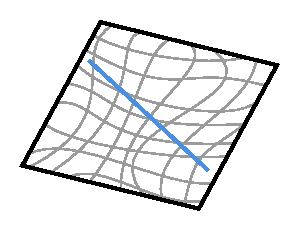
\includegraphics[width=.4\textwidth]{fig/chpt01/geodesic.pdf}
    \caption{ $\R^2$ 任意坐标系及直线}
\end{figure}

引力作用现解释为度规非闵。因为倘若存在某系使得处处 $g_{\mu\nu}=\eta_{\mu\nu}$,该系就为惯性系,而自由粒子运动为直线,说明无引力。可见即使克氏符是赝张量,其实也能体现绝对的引力现象,因为度规非闵等价于\textit{不存在}坐标系使克氏符\textit{处处}为零。只保证存在局域惯性系使克氏符严格在测地线上全零。
引力场可由时空度规描述,而前文提过,度规决定一套几何学,故\textit{引力可表为时空的几何效应},即\textbf{Lorentz几何}。
Poincaré 和 Riemann 都尝试过仅用空间几何构建引力理论,但未能成功。引力几何理论的关键就在于补上时间这一维,时间对引力亦有贡献。

测地线方程指出 $\Gamma^{\lambda}_{\mu\nu}$ 具有引力场强的意义,进而 $g_{\mu\nu}$ 具有引力势的意义。实际上的确可直接寻找度规同引力势的关系。
置一孤立场源。
研究时坐标系可取为与场源共动,比如地面系或某个遥远观者所尽可能构造的坐标系。
注意孤立系统各不影响,因而所关心场源的外引力场很弱,则该系近似为惯性系的余地很大。
并且,当远离所关心的孤立系统时,引力场是\textbf{渐弱的},即任取某种距离 $r$(如欧氏距离)后有 $g_{\mu\nu}=\eta_{\mu\nu}+O(r^{-1})$。
当然,也可直接考虑的场源质量较小。可见无论如何,都能考虑\textbf{线性近似},即与 $\eta_{\mu\nu}$ 只差小量:
\eq{
    g_{\mu\nu}=\eta_{\mu\nu}+h_{\mu\nu},\quad |h_{\mu\nu}|\ll 1.
}
从而能在 $\eta_{\mu\nu}$ 的惯性系中将引力近似解释为 $h_{\mu\nu}$。在弱场意义上,假若所研究的对象还\textbf{低速},即 $h_{\mu\nu,0}=0$ 且试验质点近似静止,便可认为 Newton 理论成立。
这其实也是对一套新理论的基本要求,称为\textbf{Newton 极限}。
由归一性知
\eq{
    U^\mu=(-g_{00})^{-1/2}\delta^\mu_0,
}
从而一阶意义上 $U^\mu=\delta^\mu_0$。此时测地线方程为 $\dv*{U^\mu}{\tau}=-\Gamma_{00}^\mu= \frac 12 g^{\mu\nu} g_{00,\nu}=\frac 12 \eta^{\mu\nu} h_{00,\nu}$,则 $-\del^i\phi=\dv*[2]{x^i}{t}=\frac 12 \delta^{ij} h_{00,j}$,故
\eq{
    h_{00}=-2\phi,\quad g_{00}=-(1+2\phi),
}
其中规定 $h_{\mu\nu},\phi$ 在无穷远处均衰减至零。


\subsection{Levi-Civita 联络}\label{sec:co-di}

可以看到 $\dv*{U^\lambda}{\tau}$ 或偏导数只有 Lorentz 协变性而无广义协变性。我们将 4-加速理解为对 4-速求一种保持张量协变性的导数,这种导数只在局域惯性系中才还原为 ${\d\tilde U^\alpha}/{\d\tau}$。不妨记 $D/\d\tau$,即 $A^\lambda={D U^\lambda}/{\d\tau}=\dv*{U^\lambda}{\tau}+\Gamma^\lambda_{\mu\nu}U^\mu U^\nu$。
$D$ 称为\textbf{绝对微分}或\textbf{协变微分},日文译为\textbf{共变}。$D/\d\tau$ 称为\textbf{沿线协变导数}。换言之 $D/\d\tau$ 总保持其作用对象的广义协变性,而只在局域惯性系中还原回 $\d/\d\tau$。
相应于 $\dv*{\tau}$ 可按全微分关系表为若干坐标偏导 $\del_\nu$ 的线性组合,对 $D/\d\tau$ 而言亦有\textbf{协变导数} $\nabla_\mu$ 的概念\footnote{注意与规范协变导数 $D_\mu$ 相区分。}。一般只讨论张量的协变导数。比如对逆变矢量 $V^\mu$ 而言有 ${D V^\mu}/{\d\tau}=:\nabla_\nu V^\mu {\d x^\nu}/{\d \tau}=U^\nu\nabla_\nu V^\mu$,且可有类似的分号简记:$V^\mu{}_{;\nu}=\nabla_\nu V^\mu :={V^\mu}{}_{,\nu}+\Gamma^\mu_{\sigma\nu}V^\sigma$。常把多出的克氏符项称为对偏导数的“协变性修正”。
协变导数的优势是无需借助于曲线及其参数,但劣势是某点的 $ V^\mu{}_{;\nu}$ 要求 $V^\mu$ 在该点邻域都有定义,而沿线求导只要求曲线上的邻域有定义。

其它张量的协变导数仍可从局域惯性系出发,按张量变换律推出,但更简单地关注如下事实:首先,就标量 $f$ 而言,由全微分或链式法则可知,偏导已有广义协变性,故 $f_{;\nu}=f_{,\nu}$。
其次,从局域惯性系的偏导可知,任意协变导数应具有\textbf{Leibniz 法则},便可从标量、逆变矢量的协变导数及 Leibniz 法则推出一般情形。首先就协变矢量而言,构造标量 $V^\mu\omega_\mu$,则对任意 $V^\mu$ 有 $(V^\mu\omega_\mu)_{;\nu} = (V^\mu\omega_\mu)_{,\nu} $,用 Leibniz 法则拆项并代入矢量协变导数有 $V^\mu \omega_{\mu;\nu}+\omega_{\mu}\Gamma^\mu_{\nu\sigma}V^\sigma=V^\mu(\omega_{\mu;\nu}+\Gamma^\sigma_{\mu\nu}\omega_{\sigma})=V^\mu \omega_{\mu,\nu}$,因此 $\omega_{\mu;\nu}=\omega_{\mu,\nu}-\Gamma^\sigma_{\mu\nu}\omega_\sigma$。
按此方法可得 $(k,l)$-张量的协变导数为
\begin{align}\label{eq:cov-tens}
     T^{\mu_1\cdots\mu_k}{}_{\nu_1\cdots\nu_l;\lambda}&=
      T^{\mu_1\cdots\mu_k}{}_{\nu_1\cdots\nu_l,\lambda}\nonumber\\
&+\sum_{i=1}^k \Gamma^{\mu_i}_{\lambda \sigma} T^{\mu_1\cdots\sigma\cdots\mu_k}{}_{\nu_1\cdots\nu_l}-\sum_{j=1}^l\Gamma^{\sigma}_{\lambda \nu_j} T^{\mu_1\cdots\mu_k}{}_{\nu_1\cdots\sigma\cdots\nu_l}.
\end{align}
在记忆时注意,此即先填上一个偏导,再对所有指标依次添加相应的克氏符修正项(正负取决于指标上下),并满足指标平衡。

式 \eqref{eq:g=gamma} 说明度规的协变导数为零:$g_{\mu\nu;\sigma}= {g_{\mu\nu,\sigma}}-g_{\mu\lambda}\Gamma^\lambda_{\sigma\nu}-g_{\nu\lambda}\Gamma^\lambda_{\sigma\mu}=0$,
称为\textbf{度规适配性}(metric-compatibility)。进而可直接在任意坐标系下证明 $A^\mu,U^\nu$ 正交: $A^\mu U_\mu=\frac 12  \frac{D}{\d\tau} (g_{\mu\nu} U^\nu U^\mu)=0$。
数学上称满足 $D V^\mu/\d\tau=0$ 的逆变矢量 $V^\mu$ 在做\textbf{平行移动}(parallel transport)或\textbf{Levi-Civita 移动}。切矢 $T^\mu=\dv*{x^\mu}{\sigma}$ 沿其自身平行移动的曲线称为\textbf{测地线}(geodesic),即 $T^\mu\nabla_\mu T^\lambda =0$。
此称\textbf{测地线方程}。可见自由落体运动就是引力度规下的测地线。假设 $V^\mu,W^\nu$ 沿某条线平行移动,则内积沿线恒定:$\frac{D}{\d\tau}(V^\mu W_\mu)=0$。
就单个 $V^\mu$ 而言说明模方恒定,的确可看作一种“平行移动”。
\begin{figure}[ht]\centering
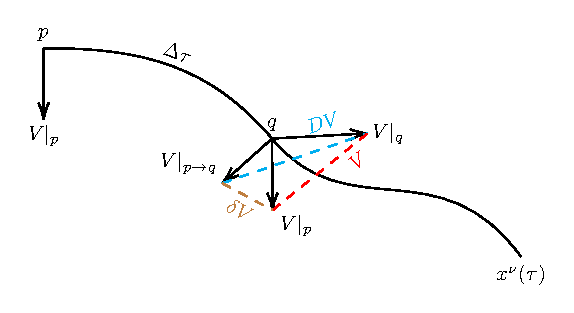
\includegraphics[width=.6\textwidth]{fig/chpt01/covar-deri.pdf}
    \caption{图中 $\Delta\tau$ 等差值均夸大}\label{covar-deri}
\end{figure}
不妨考察其直观含义。如图 \ref{covar-deri},设某曲线 $x^\nu(\tau)$ 上 $p$ 为参数零点,而邻近点 $q$ 的参数记作 $\Delta\tau$(可正可负)。若矢量场 $ V$ 至少在 $p,q$ 线段上有定义,便可讨论 $p$ 处沿线导数算符。设矢量场在 $p,q$ 分别取值 $ V|_p, V|_q$,则
\[\eval{\dv{V^\mu}{\tau}}_p=\lim_{\Delta\tau\to 0}\frac{V^\mu|_q-V^\mu|_p}{\Delta\tau}\]
是直接比较 $V|_q,V|_p$,但二者隶属不同切空间,差值 $\d V$ 意义不明。这是 $\d V^\mu/\d\tau$ 不协变的直观理解。欲画出 $\d V$,需将矢量照搬至同一点作差。不妨考虑 $q$ 点。图中 $q$ 点的 $V|_p$ 为照搬结果,故 $\d V$ 标注如图。另一方面,
\[\eval{\frac{DV^\mu}{\d\tau}}_p=\lim_{\Delta\tau\to 0}\frac{V^\mu|_q-V^\mu|_p}{\Delta\tau}+\Gamma^\mu_{\lambda\nu}|_p  V^\nu|_p \lim_{\Delta\tau\to 0} \frac{\Delta x^\lambda}{\Delta\tau}=\lim_{\Delta\tau\to 0}\frac{V^\mu|_q-V^\mu|_{p\to q}}{\Delta\tau},\]
其中 $V^\mu|_{p\to q}=V^\mu|_p-\Gamma^\mu_{\lambda\nu}|_p  V^\nu|_p \Delta x^\lambda$。
可见 $DV^\mu/\d\tau$ 是求 $V|_q$ 与 $q$ 处新矢量 $V|_{p\to q}$ 之差。这样 $D V$ 表为如图。$\delta V$ 为 $V|_{p\to q}, V|_p$ 之差。由上式或图示知 $\delta V^\mu = \d V^\mu-D V^\mu=-\Gamma^\mu_{\sigma\nu}V^\sigma\d x^\nu$,这便是克氏符项所给出的修正。$V|_{p\to q}$ 其实就是平移移动的结果。为看出这一点,只需令 $V$ 自己就处处按这种方式移动,则 $D V^\mu/\d\tau=0$。

设定时空上的逆变矢量场是给各时空点赋予其相应的逆变矢量,一个逆变矢量是绑定于一点的,故任意两点 $p,q$ 处各自的逆变矢量本无关联。然而给定某 $p,q$ 间之曲线,可通过矢量的平行移动,将两个切空间联系起来。因此 $\nabla_\nu$ 又被称为\textbf{联络}(connection)。附录 \ref{appx:curvature} 给出了一般的联络定义,每种联络都有相应的\textbf{联络系数} $\hat{\Gamma}^\lambda_{\mu\nu}$,相应测地线用 $U^\nu\hat\nabla_\nu U^\mu=0$ 定义。设\textbf{挠率}(torsion)为 $T^\lambda{}_{\mu\nu}:=2\Gamma^\lambda_{[\mu\nu]}$,它靠着克氏符作差消除了这一项,故是张量。按式 \eqref{Christoffel} 定义的联络系数满足 $T^\lambda{}_{\mu\nu}=0$,这种联络称为\textbf{无挠}(torsion-free)\textbf{联络}。度规适配的无挠联络称为\textbf{Levi-Civita 联络}。由此二条件可证联络系数正是克氏符,故 Levi-Civita 联络存在且唯一。
我们主要研究\textbf{无挠时空},必须选择 Levi-Civita 联络。一是出于方便,二是每一时空点都有局域的 Lorentz 不变性。若要求还要涵盖局域的平移对称性,即总地要求局域 Poincaré 对称性,需要考虑有挠联络。这仍能遵循等效原理,因为测地线方程中 $U^\mu U^\nu=U^{(\mu} U^{\nu)}$,只要求对称部分 $\Gamma^\lambda_{(\mu\nu)}$ 等于 \eqref{Christoffel} 式也仍使粒子在引力下走测地线。同理 $g_{[\mu\nu]}\ne 0$ 亦可,但为方便总选二阶对称张量作为度规。 

\subsection{广义不变性}

Einstein 想要借由广义协变性发展出一套坐标选择无关的理论,以\textit{尽可能排除人为因素}。但协变性对约束引力理论是不够的,事实上还需要不变性。首先,将 Lorentz 不变性中的常数不变推广到所谓的\textbf{绝对对象}(absolute object),即与物质状态无关的各种量,除了常数 $c=G=1,\hbar/2$,最重要的是还包括更高指标的,比如 Jacobi 矩阵元 $\pdv*{x^\mu}{x'^\nu}$。与物质状态有关而可变的称\textbf{动力学对象}(dynamical object),例如粒子的位置和动量、场的场强和能量密度等。给定任何物理方程,按定义总能把其中的量分为这两类。\textbf{广义不变性}就是说,\textit{任何物理定律有广义协变性,且方程中的绝对对象在任意坐标变换下相同},就能决定了哪些绝对对象才可以出现于方程中。
Jacobi 矩阵元这种一定是绝对对象的项就不能出现了。一个描述物理定律的方程必须是指标平衡的张量方程,才可在坐标变换下消除 Jacobi 矩阵元,进而一种坐标系对应方程的一种表达,并保持广义不变性,不会同时出现两种坐标系符号。

广义不变性所提出的要求当然高于 Lorentz 不变性。
$c=1,\hbar$ 和 $\eta_{\mu\nu}$ 有资格成为 Lorentz 不变性下的绝对对象,但 $\eta_{\mu\nu}$ 不能在任意坐标变换下严格不变,它可变成某个 $g_{\mu\nu}$。在引力理论中,由于 $g_{\mu\nu}$ 必须出现,我们只能期望 $g_{\mu\nu}$ 是动力学对象,它所满足的某个方程才能有广义不变性。结合等效原理,我们知道这是物质源产生引力场的定量关系,称为\textbf{引力场方程}或\textbf{场方程}。当今主流上称这套理论为\textbf{广义相对论}。当然,最初他认为“广义相对”一词来自广义协变性,但现在看来是来自等效原理和广义不变性。为避免歧义,Wheeler 很早就提议将该理论称为\textbf{几何动力学}(geometrodynamics)以强调其本质,即与物质相互作用的动力学几何。 

正如运动方程是 $x^\mu(\tau)$ 的常微分方程,场方程是 $g_{\mu\nu}$ 的偏微分方程,且根据广义不变性,它应是张量方程,其中的张量由度规及其偏导构造。记自由引力场、物质场的总拉氏密度为 $\mathcal L$。尽管可在局域惯性系中消除引力,但作为物理规律的作用量是不能在局域惯性系中失去耦合性的,它必须是标量场。取局域惯性系 $\{\xi\}$ 并置 $S=\int \mathcal L \d[4]{\xi}$。
体元变换 $\d[4]x =\tilde J \d[4]{\xi}$ 的 $\tilde J$ 能用度规行列式表示。记度规在 $\{x\}$ 系的行列式是 $g:=\det(g_{\mu\nu})$。对 $g_{\mu\nu}$ 的定义取行列式有
\eq{
    g=\det(\pdv{\xi^\alpha}{x^\mu})\det(\pdv{\xi^\beta}{x^\nu})\det(\eta_{\alpha\beta})=-\tilde J^{-2},
}
假设坐标变换保持右手性,则
\eq{
    \sgn g=-1\implies 1/\tilde J=\sqrt{-g}\implies S=\int \mathcal L \sqrt{-g}\d[4]{x},
}
可见 $g$ 虽与坐标选择有关,但在变换下一定保号,即引力度规的行列式总是负的(无关号差)。规定\textbf{适配体元} $D^4 x$ 只在局域惯性右手系 $\{\xi\}$ 中表为 $\d[4]\xi$,就有 $D^4 x=\sqrt{-g}\d[4]{x}$。
可以考虑用张量缩并获得标量。这种张量必须直接代表引力强弱,它不能是 $g_{\mu\nu}$ 级的,因为可用局域惯性系消为 $\eta_{\alpha\beta}$;也不能是 $g_{\mu\nu,\lambda}$ 级的,因为其可表为克氏符,在一点处可取局域惯性系使其为零。这意味着至少要考虑二阶导的构造,故最终场方程至少是二阶的。按有效性精神,先考虑有且仅有二阶的情形;且注意 Newton 引力论在低精度实验中是成立的,故广义相对论必须囊括这一理论,而 Poisson 方程恰好也是二阶的。
然暂不清楚将二阶导数作用于何物,因此要回到物理学。相比于单条测地运动,潮汐现象必须在足够大邻域内,等效原理不再适用。若欲寻求尽可能简单的定义,则该张量场\textit{在一点}就应具备潮汐意义。

\subsection{潮汐}

\begin{figure}[ht]\centering
    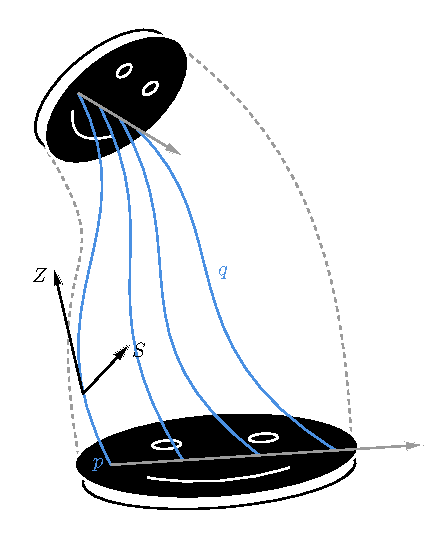
\includegraphics[width=.5\textwidth]{fig/chpt01/geo-devi.pdf}
            \caption{测地偏离}
            \label{fig:geo-devi}
\end{figure}
设物质场与引力场的最小耦合项为 $S_M=\int\mathcal L_M D^4{x}$,并通常令
\eq{
    S=S_G+S_M=\int\left(\frac{1}{2\kappa}\mathcal L_G +\mathcal L_M\right)\sqrt{-g}\d[4]{x},
}
其中 $\kappa$ 是按习惯设置的待定耦合常数。
为构造 $\mathcal L_G$,先找到具有潮汐意义的张量。考虑任意流体,如图 \ref{fig:geo-devi},对共动系的空间部分讨论如下。任选一条不自交的光滑曲线,使其上任一切矢都与过该点的观者相交,称为\textbf{横向曲线}。用 $s$ 参数化横向曲线,则与其相交的观者对应了交点参数,即在线汇中挑出了一个\textbf{单参族},横向曲线沿各观者 4-速便扫出一张 2 维曲面,可称\textbf{世界面}(worldsheet)。设任意坐标系 $\{x\}$,则可表为 $x^\mu(\tau,s)$,其中 $\{\tau,s\}$ 可以视为共动系的子集,当然也可不要求对钟,直接约定某初始的横向曲线 $x^\mu(0,s)$。可取单参族中的一者为\textbf{基准观者}(fiducial observer),比如 $x^\mu(\tau,0)$,而 $s$ 正方向的邻近观者称其\textbf{邻居}(neighbor),或者用\textbf{偏离矢量}(separation vector) $S^\mu:=\pdv*{x^\mu}{s}$ 来指代,其大小象征相对间距。这样 $x^\mu(\tau,s)$ 上建立了观者 4-速场 $Z^\mu:=\pdv*{x^\mu}{\tau}$ 和偏离矢量场 $S^\mu$。由链式法则,它们的确逆变。

再考虑类时测地线汇,其共动系可称\textbf{测地系}。相对加速度场表征为偏离矢量沿 4-速场的二阶协变导数 $Z^\nu \nabla_\nu(Z^\kappa \nabla_\kappa S^\lambda)$,部分书籍也采用记号 ${D^2S^\lambda}/{\d\tau^2}$。很容易展开证明 $Z^\nu\nabla_\nu S^\mu=S^\nu\nabla_\nu Z^\mu$,则
\begin{align}
    Z^\nu \nabla_\nu(Z^\kappa \nabla_\kappa S^\lambda)&= Z^\nu \nabla_\nu\left(S^\kappa\nabla_\kappa Z^\lambda\right) = \left(Z^\nu \nabla_\nu S^\kappa\right)\nabla_\kappa Z^\lambda+Z^\nu S^\kappa \nabla_\nu \nabla_\kappa Z^\lambda\nonumber\\
    &= \left(S^\nu \nabla_\nu Z^\kappa\right)\nabla_\kappa Z^\lambda+Z^\nu S^\kappa\left(\nabla_\kappa \nabla_\nu Z^\lambda+2\nabla_{[\nu}\nabla_{\kappa]}Z^\lambda\right)\nonumber\\
    &=S^\kappa\nabla_\kappa\left(Z^\nu \nabla_\nu Z^\lambda\right) +2Z^\nu S^\kappa\nabla_{[\nu}\nabla_{\kappa]}Z^\lambda\nonumber\\
    &=R^\lambda{}_{\mu\nu\kappa}  Z^\mu  Z^\nu S^\kappa,\quad R^\lambda{}_{\mu\nu\kappa}Z^\mu:= 2\nabla_{[\nu}\nabla_{\kappa]}Z^\lambda,
\end{align}
称为\textbf{测地偏离}(geodesic deviation)\textbf{方程},解 $S^\lambda$ 称为\textbf{Jacobi 场}。$R^\lambda{}_{\mu\nu\kappa}$ 表征潮汐形变程度,是 $g_{\mu\nu,\lambda\kappa}$ 级的张量:式左是协变导数,式右 $Z^\mu,S^\kappa$ 是逆变矢量。这称为\textbf{Riemann 张量}。
Jacobi 场固然无穷多种,但我们感兴趣满足对钟正交性的 Jacobi 场。实际上,任意 $S^\lambda$ 总可投影为正交 Jacobi 场
\eq{\eta^\lambda=S^\lambda+Z_\nu S^\nu Z^\lambda,}
而只要初始横向曲线与线汇正交,则此后都保持正交:$Z^\nu \nabla_\nu\left(S^\mu Z_\mu\right) =Z_\mu Z^\nu \nabla_\nu S^\mu=Z_\mu S^\nu \nabla_\nu Z^\mu=\frac{1}{2} S^\nu \nabla_\nu\left(Z_\mu Z^\mu\right)=0$。
可以展开定义式:计算 $\nabla_\nu\nabla_\kappa V^\lambda$ 时注意勿先展开内部,将 $\nabla_\kappa V^\lambda$ 视作整体以避开对克氏符求导,最后代入无挠性得
    \eq{\label{eq:Rie-cur}
         R^\lambda{}_{\mu\nu\kappa}:=-2\Gamma^\lambda_{\mu[\nu,\kappa]}+2\Gamma^\lambda_{\sigma[\nu} \Gamma^\sigma_{\kappa]\mu}.
    }
故 $R^\lambda{}_{\mu\nu\kappa}$ 表征度规的非闵程度。

再考虑 Newton 极限。取测地系 $\{\xi\}$ 并设正交 Jacobi 场 $\eta^\mu$。显然 $\tilde Z^\mu=\delta^\mu_0$ 且 $\tilde\eta^0=0$。根据定义显然有反称性
\eq{\label{eq:R_..ab=-}
    {R^\lambda}_{\mu\nu\kappa}={R^\lambda}_{\mu[\nu\kappa]},
}
则测地偏离方程在共动系下写作 $\pdv[2]{\tilde\eta^i}{t}=-\tilde R^i{}_{0 j 0} \tilde\eta^j$。
设每条测地线足够低速,故共动系成为了惯性系,进而 $\pdv[2]{\tilde\eta^i}{t}\approx \tilde\eta^j \pdv{\xi^j}\pdv[2]{\xi^i}{t}=-\tilde\eta^j \pdv{\xi^j}\tilde\del^i\phi$。
从而 $\tilde R^\sigma{}_{0 \sigma 0}=\tilde R^i{}_{0 i 0} \approx \tilde\partial_i\tilde\partial^i{\phi}$。可见 $R_{\mu\nu}:={R^\sigma}_{\mu\sigma\nu}$ 很有意义,称为\textbf{Ricci 张量}。
也可从 $g_{00}=-(1+2\phi)$ 及 $R_{\mu\nu}$ 定义得 $\tilde R_{00}=-\frac 12 \nabla^2 g_{00}=\nabla^2\phi$。
还可尝试展开。首先可证线性代数中的 Jacobi 公式:
\[
    \partial_\lambda g=\pdv{g}{g_{\sigma\nu}}g_{\sigma \nu,\lambda}=\pdv{(g\delta_\sigma^\mu)}{g_{\sigma\nu}}g_{\mu \nu,\lambda} =g^{*\gamma\mu}\pdv{g_{\sigma\gamma}}{g_{\sigma\nu}} g_{\mu \nu,\lambda}=gg^{\gamma\mu}\delta^\nu_\gamma g_{\mu \nu,\lambda}=g g^{\mu \nu} g_{\mu \nu,\lambda},
\]
其中 $(g^{*\mu\nu})$ 是 $(g_{\mu\nu})$ 的伴随,具有性质 $g\delta_\sigma^\mu=g_{\sigma\gamma}g^{*\gamma\mu}$ 和 $g^{*\mu\nu}=gg^{\mu\nu}$。注意伴随(转置)矩阵元是相应代数余子式,当然有 $\pdv*{g^{*\gamma\mu}}{g_{\sigma\nu}}=0$。进而\textbf{缩并克氏符}为
\eq{
\Gamma_{ \sigma\mu}^\sigma=\frac{1}{2} g^{\sigma \kappa}\left( g_{\sigma \kappa,\mu}+ 2 g_{\mu [\kappa,\sigma]}\right)=\frac{1}{2} g^{\sigma \kappa}  g_{\sigma\kappa,\mu}=\frac{1}{2g}\partial_\mu g=\partial_\mu\ln\sqrt{-g}.
}
故
\eq{
    R_{\mu\nu}=\Gamma^\sigma_{\mu\nu,\sigma}-(\ln\sqrt{-g})_{,\mu\nu}+(\ln\sqrt{-g})_{,\kappa}\Gamma^\kappa_{\mu\nu}-\Gamma^\kappa_{\sigma\mu}\Gamma^\sigma_{\kappa\nu}.
}
可有进一步的缩并,即 $R_{\mu\nu}$ 的迹
\eq{
    R:=R^\mu{}_\mu=g^{\mu\nu}R_{\mu\nu}.
}
此即一个足够简单的 $g_{\mu\nu,\lambda\kappa}$ 级的标量,称为\textbf{Ricci 标量}。

现可给出实验操作意义的局域惯性系的定量标准。数学上固然要求局域惯性系严格建立在测地线上:假若克氏符在邻域 $U$ 内等于零,则借助邻域按 \eqref{eq:Rie-cur} 式得在线上 $R^\lambda{}_{\mu\nu\kappa}=0$,矛盾。只要邻域足够大,$R^\lambda{}_{\mu\nu\kappa}$ 便可测量。但观者往往又需借助时空邻域进行实验,好在只要 $U$ 尺寸数量级远小于 $1/\sqrt{R}$,同时也远小于其测量精度时,即使时空范围未严格至测地线,但 $R^\lambda{}_{\mu\nu\kappa}$ 也在精度范围内为零。当然,若实验范围较大或仪器精度够高,还是可以测量潮汐,见 \ref{sec:eq-prin} 节。

最小耦合指出可取 $\mathcal L_G=R$。下面研究变分。为简便运算,选择对 $g^{\mu\nu}$ 而非 $g_{\mu\nu}$变分,则 $\var(R\sqrt{-g})$ 即涉及 $g^{\mu\nu},R_{\mu\nu},\sqrt{-g}$ 三个部分。
首先是 $\delta\sqrt{-g}$。注意 $\delta^{\mu}_{\nu}=g^{\mu\lambda}g_{\lambda\nu}$ 可得 $0=g^{\mu\lambda}\var g_{\lambda\nu}+g_{\lambda\nu}\var g^{\mu\lambda}$,故
\eq{
\var g=gg^{\mu\nu}\var g_{\mu\nu}=-g g_{\mu\nu}\var g^{\mu\nu},\quad \delta \sqrt{-g}=-\frac12\sqrt{-g}g_{\mu\nu}\delta g^{\mu\nu}.
}
其次计算 $\var R_{\mu\nu}$。取局域惯性系有 $\delta\tilde R_{\alpha\beta} = \tilde\del_\sigma(\delta\tilde\Gamma^\sigma_{\alpha\beta})-\tilde\del_\beta(\delta\tilde \Gamma^\sigma_{\alpha\sigma}) = \nabla_\sigma(\delta\tilde\Gamma^\sigma_{\alpha\beta})-\nabla_\beta(\delta\tilde \Gamma^\sigma_{\alpha\sigma})$。
注意,虽克氏符不是张量,但克氏符变分是张量(作差消去非协变部分),故任意坐标系下有如下\textbf{Palatini 公式}
\eq{
\delta R_{\mu \nu}=2\nabla_{[\lambda}\delta \Gamma_{\nu]\mu}^\lambda,
}
于是 $g^{\mu\nu}\var R_{\mu\nu}=2 \nabla_{[\lambda}( g^{\mu\nu} \delta \Gamma_{\nu]\mu}^\lambda) =2\nabla_\lambda(g^{\mu [\nu} \delta \Gamma_{\mu \nu}^{\lambda]})$,其积分为边界项,舍去后有
\eq{\var \int R\sqrt{-g}\d[4]{x} 
\simeq\int G_{\mu\nu} \var g^{\mu\nu} \sqrt{-g}\d[4]{x},\quad G_{\mu\nu}:=R_{\mu\nu}-\frac 12 g_{\mu\nu} R.}
$G_{\mu\nu}$ 称\textbf{Einstein 张量}。还可有 $G:=g^{\mu\nu}G_{\mu\nu}=R-\frac{1}{2}\delta^\mu_\mu R=-R\Rightarrow R_{\mu\nu}=G_{\mu\nu}-\frac 12 g_{\mu\nu} G$。这里没有引入物质场,因此自由引力场在最小耦合意义上满足 $G_{\mu\nu}=0$ 即 $R_{\mu\nu}=0$,称\textbf{真空方程}(vacuum equation)。闵氏度规显然是一个解。
真空方程已能描述很多引力现象,因为场源往往限制在很小的区域内,而外部区域真空,可允许试验粒子运动。

再考虑物质部分 $S_M$。约定 $\delta S_M =-\frac{1}{2} \int T_{\mu \nu} \delta g^{\mu \nu} D^4{x}$,即令
\eq{
T_{\mu \nu}:=-\frac{2}{\sqrt{-g}}\fdv{(\mathcal L_M\sqrt{-g})}{g^{\mu\nu}}=-2\fdv{\mathcal L_M}{g^{\mu\nu}}+g_{\mu\nu}\mathcal L_M,
}
则 $\var S\simeq\frac{1}{2\kappa}\int\left(G_{\mu\nu}-\kappa T_{\mu\nu}\right)\var g^{\mu\nu}\sqrt{-g}\d[4]{x}=0\Rightarrow G_{\mu\nu}=\kappa T_{\mu\nu}$,此即引力场方程的一般形式。可以预料 $T_{\mu\nu}$ 与场源质量(因而能量、动量)有关。还可有
\[ 
R_{\mu\nu}=G_{\mu\nu}-\frac 12 g_{\mu\nu} G=\kappa\left(T_{\mu\nu}-\frac12 g_{\mu\nu}T\right),
\]
称为\textbf{反迹}(trace-reversed)表达。当然,$T_{\mu\nu}$ 的具体意义和 $\kappa$ 的值还需落实。

\subsection{曲率的性质}

数学上称 $R^\lambda{}_{\mu\nu\kappa}$ 为\textbf{Riemann 内禀曲率}(intrinsic curvature)或\textbf{曲率}。$1/\sqrt{R}$ 相当于曲率半径。曲率为零时称度规为\textbf{平直的}(flat),非零时称\textbf{弯曲的}(curved),物理学可以借用这些词而称\textbf{时空曲率},时空分为\textbf{平直时空}和\textbf{弯曲时空}。渐弱度规也称\textbf{渐近平直}(asymptotically flat)度规。下面解释曲率称呼的意义。我们预先\textit{规定}欧氏空间是平直的,以它为基准可判断某条线、某张面的弯曲。考虑一个球面,其上任意切矢沿自身平移所得测地线即过球心的大圆。设从赤道某两处垂直延伸两条大圆弧,它们的间距逐渐缩短并交于极点。在一张平面上,初态平行的直线不可能改变间距。矢量平行移动就是相对于路径各处邻域平移,然而考虑将扇形围成圆锥面,矢量沿着包含尖端的环路平行移动后,与原矢量不重合,而直观上尖端处有曲率,故曲率非零时,平行移动结果往往与路径有关。
另一方面,按如下操作可计算球面上的线元:先用球坐标 $\{r,\theta,\phi\}$ 改写欧氏度规为
\eq{
    \d\l^2=\d r^2+r^2\d\Omega^2,\quad \d\Omega^2:=\d\theta^2+\sin^2\theta\,\d\phi^2,
}
当然,此处 $\Omega$ 不是立体角(solid angle),立体角满足的是 $\d\Omega=\sin\theta \d\theta\d\phi$。再取 $r=R$ 就有所谓的\textbf{球面度规} $\d\l^2=R^2\d\Omega^2$,由此可计算球面曲率不为零。像这样,约定背景空间中\textbf{嵌入}(imbedded)\textbf{曲面}的长度是用背景度规衡量的,这称为背景度规的\textbf{诱导}(induce)\textbf{度规}。可见度规在非欧或非闵时,内禀曲率非零而使测地间隔变化。但内禀曲率其实只由度规和坐标系计算而来,甚至无需嵌入某个高维背景来定义度规和曲率——对于四维时空,我们就只能抛弃嵌入思想来想象它。内禀曲率只反应内禀的弯曲程度而与曲面本身无关:球面在内禀意义下弯曲,但圆柱面在内禀意义下平直(借柱坐标发现诱导度规平直),尽管它在直观上弯曲。数学上,描述圆柱面这种对象的弯曲程度就需要嵌入思想,称为\textbf{外}(extrinsic)\textbf{曲率}。一个直观理解是,凡能连续地展平的曲面,尽管外曲率可不为零,但内禀曲率为零;真正不可连续展平的曲面内禀曲率、外曲率都非零。读者可观察纸塑地球仪是如何尝试将平面纸张大致贴合球面的。


曲率具有若干性质。首先注意无挠性导致 $\nabla_{[\nu}\nabla_{\kappa]}(V^\mu \omega_\mu)=0$,则可得
\eq{
    2\nabla_{[\nu}\nabla_{\kappa]} \omega_\mu = - R^\lambda{}_{\mu\nu\kappa} \omega_\lambda.
}
前文已提过反称性 \eqref{eq:R_..ab=-} 式,
其次是所谓的\textbf{Ricci 循环恒等式}(cyclic identities)
\eq{{R^\lambda}_{[\mu\nu\kappa]}=0.}
证明只需默认无挠性,并运用取测地系的技巧(其中 $\tilde R^\lambda{}_{\mu\nu\kappa}=-2\tilde \Gamma^\lambda_{\mu[\nu,\kappa]}$)。

\textbf{降指标 Riemann 曲率} $R_{\lambda\mu\nu\kappa}:=g_{\lambda\sigma}{R^\sigma}_{\mu\nu\kappa}$ 是一个常用概念,它与原先 ${R^\lambda}_{\mu\nu\kappa}$ 有等价的独立分量数,因此有时也称 Riemann 曲率。它使我们能看到更多性质,如反称性
\eq{
    R_{\lambda\kappa\mu\nu}=R_{[\lambda\kappa]\mu\nu}.
}
直接证明它亦可从无挠性和测地系入手。由此可知
$R_{\mu\nu}$ 是 ${R^\lambda}_{\mu\nu\kappa}$ 唯一非平凡缩并,另两种缩并是平凡的:$R^\sigma{}_{\mu\nu\sigma}=-R^\sigma{}_{\mu\sigma\nu}=-R_{\mu\nu}$,以及 $R^\sigma{}_{\sigma\mu\nu}=g^{\lambda\sigma}R_{\lambda\sigma\mu\nu}=g^{(\lambda\sigma)}R_{[\lambda\sigma]\mu\nu}=0$。
最后是前一对指标和后一对指标的对称性:
\eq{
    R_{\mu\nu\lambda\kappa}=R_{\lambda\kappa\mu\nu}.
}
同理默认无挠性并取测地系即可。包括式 \eqref{eq:R_..ab=-} 在内的这四条性质是我们能得到的所有代数性质了。

由 ${R^\lambda}_{\mu\nu\kappa}={R^\lambda}_{\mu[\nu\kappa]}$ 可知 Ricci 恒等式还有如下形式:
\eq{
    R^\lambda{}_{\mu\nu\kappa}+R^\lambda{}_{\nu\kappa\mu}+R^\lambda{}_{\kappa\mu\nu}=0.
}
注意,上式若存在相同指标,则总与另三条性质重复,故常考虑指标各不相同的非平凡 Ricci 恒等式。直观上,四维时空的 Riemann 曲率的分量有 $4^4=256$ 之多,但以上性质使其分量往往重复或为零。利用简单的组合数学可知其实际只有 20 个独立分量。由此还可证明,Riemann 曲率是唯一可由度规二阶导线性组合而成的张量。细节放入附录 \ref{appx:curvature}。故我们选择用 Riemann 曲率描述引力。

可用缩并将 Riemann 曲率进行压缩从而保留有用数据。前文已说明,初步缩并的唯一有用结果是 Ricci 曲率。可直接根据定义得
\eq{
    R_{\mu\nu}=R_{(\mu\nu)}.
}
亦可根据 $R_{\mu\nu\lambda\kappa}=R_{\lambda\kappa\mu\nu}$ 有 $R_{\mu\nu}=g^{\sigma\lambda}R_{\sigma\mu\lambda\nu}=g^{\sigma\lambda}R_{\lambda\nu\sigma\mu}=R_{\nu\mu}$。
此外,Ricci 标量也是非平凡缩并。虽然这不是唯一能从 $g_{\mu\nu},R^\lambda{}_{\mu\nu\kappa}$ 得到的非平凡标量(见附录 \ref{appx:curvature}),但确实是足够简单的一个。

除了上述纯代数性质之外,Riemann 曲率还满足一个微分恒等式:
\eq{
    R^\lambda{}_{ \mu [\sigma\nu ; \kappa]}=0,
}
这称为\textbf{Bianchi 恒等式}。可直接用无挠性和测地系证明之。
由 ${R^\lambda}_{\mu\nu\kappa}={R^\lambda}_{\mu[\nu\kappa]}$ 可知 Bianchi 恒等式还有如下形式:
\eq{
    R^\lambda{}_{ \mu \sigma\nu ; \kappa}+R^\lambda{}_{ \mu \nu\kappa;\sigma}+R^\lambda{}_{ \mu \kappa\sigma;\nu}=0.
}
对上式缩并 $\lambda,\sigma$ 再用 $g^{\mu\kappa}$ 升指标,且注意 $g^{\mu\kappa} R_{\lambda \mu\nu\kappa}=g^{\mu\kappa} R_{\mu\lambda\kappa \nu}=R^{\kappa}{}_{\lambda\kappa \nu}=R_{\lambda\nu}$,则 $\nabla^{\mu} R_{\mu\nu}+ \nabla^\lambda R_{\lambda\nu}-\del_\nu R=0\Rightarrow\nabla^{\mu} R_{\mu\nu}=\frac 12\del_\nu R$,故 $G_{\mu\nu}$ 无散:
\eq{
    \nabla^{\mu}G_{\mu\nu}=0.
}

\subsection{Einstein 方程}

考虑尘埃及其 4-速场 $Z^\mu$,
只需取局域惯性系即知质量守恒等价为 $\nabla_\nu(\mu^* Z^\nu)=0$。而协变散度可直接用偏导表示。
逆变矢量的散度为
\eq{
 V^\mu{}_{;\mu}= V^\mu{}_{,\mu}+\Gamma_{ \mu\nu}^\mu V^\nu=V^\mu{}_{,\mu}+V^\mu \partial_\mu\ln\sqrt{-g} =\frac{1}{\sqrt{-g}} \del_\mu\left(\sqrt{-g} V^\mu\right).
}
结论是任意系有 $\del_\nu(\mu^* Z^\nu\sqrt{-g})=0$,这给出 $\var(\mu^* Z^\nu\sqrt{-g})=0$ 的理由前文已述。
注意 $\var(Z^\mu Z_\mu)=\var(-1)=0$,则易得 $\var Z^\mu=\frac 12 Z_\nu \var g^{\mu\nu}$,故
\eq{
    \var(\mu^*\sqrt{-g})=\frac 12 \mu^* Z_\mu Z_\nu \sqrt{-g}\var g^{\mu\nu}\implies T_{\mu\nu}=\mu^* Z_\mu Z_\nu.
}
同理,可取 $\delta S_M =\frac{1}{2} \int T^{\mu \nu} \delta g_{\mu \nu} D^4{x}$ 而有
\eq{
T^{\mu \nu}:=\frac{2}{\sqrt{-g}}\fdv{(\mathcal L_M\sqrt{-g})}{g_{\mu\nu}}=2\fdv{\mathcal L_M}{g_{\mu\nu}}+g^{\mu\nu}\mathcal L_M=g^{\mu\alpha}g^{\nu\beta} T_{\alpha\beta}.
}
那么当然 $T^{\mu\nu}=\mu^* Z^\mu Z^\nu$。可见 $T^{00}=T_{00}=\mu$ 即能量密度,$T^{i0}=T^{0i}=\mu u^i $ 即动量密度或能流密度,而 $T^{ij}=\mu u^i u^j$ 即动流密度或应力张量。因此,$T^{\mu\nu}$ 称为物质场源的\textbf{4-动流密度}或\textbf{能动张量}(energy-momentum tensor)。$\nabla^{\mu}G_{\mu\nu}=0$ 要求
\eq{
    \nabla_\mu T^{\mu\nu}=0,
}
取 $\nu=0$ 即能量局域守恒,取 $\nu=i$ 即动量局域守恒。代入 $T^{\mu\nu}=\mu^* Z^\mu Z^\nu$,则 $\nabla_\mu T^{\mu\nu}=\mu^* Z^\mu\nabla_\mu Z^\nu$。故 $\nabla_\mu T^{\mu\nu}=0$ 等价于 $Z^\mu\nabla_\mu Z^\nu =0$,说明各质元自由落体。

考虑 Newton 极限。取共动系,$R_{\mu\nu}Z^\mu Z^\nu=\tilde R_{00}=\nabla^2\phi= 4\pi\mu^*$。另一方面 $\tilde Z^\mu=\delta^\mu_0,\tilde Z_\mu=-\delta_{\mu 0}$,则 $T_{\mu\nu}Z^\mu Z^\nu=\tilde T_{00}=\tilde T^{00}=\mu^*$。进而 $T:=g_{\mu\nu}T^{\mu\nu}=-T^{00}=-\mu^*$。由前文知 $R=-G=-\kappa T$,场方程与 $Z^\mu Z^\nu$ 缩并得 $4\pi\mu^*-\frac 12 (-1)\kappa \mu^*=\kappa\mu^*$,则
\eq{
    R_{\mu\nu}-\frac12 g_{\mu\nu} R=8\pi T_{\mu\nu},\quad \kappa=8\pi.
}
这称为\textbf{Einstein 方程}。$\frac{1}{16\pi}\int R \sqrt{-g}\d[4]{x}$ 称为\textbf{Einstein-Hilbert 作用量}。

\subsection{最小引力耦合}

现设流体带固有电荷密度 $\rho^*$,电流密度为 $J^\mu=\rho^* Z^\mu$。电荷守恒从局域惯性系出发变换为 $\nabla_\mu J^\mu = 0$,则后续对 $A_\mu,g^{\mu\nu}$ 的变分均有 $\var(J^\mu\sqrt{-g})=0$。
研究电磁场 $F_{\mu\nu}$ 的最小引力耦合。单粒子的运动方程遵循
\eq{
\delta\int \left(-m+q A_\mu U^\mu\right)\d\tau =0 \implies \frac{D P^\mu}{\d\tau}=q F^\mu{}_{\nu}U^\nu,
}
电磁场的运动方程遵循
\eq{
    \delta\int\left(-\frac{1}{16\pi} F^{\mu\nu} F_{\mu\nu}+A_\nu J^\nu\right)\sqrt{-g}\d[4]{x}=0 \implies \nabla_\mu F^{\mu\nu}=-4 \pi J^\nu,
}
而 $F_{\mu\nu}$ 的定义和无挠性自动给出 $F_{\mu\nu}=2\nabla_{[\mu}A_{\nu]}=2\del_{[\mu}A_{\nu]}$,则
\eq{
    F_{[\mu\nu;\lambda]}=F_{[\mu\nu,\lambda]}=0.
}
Lorenz 规范从局域惯性系出发变换为 $\nabla^\mu A_\mu =0$,则引力耦合的 d'Alembert 方程为
\begin{align}
    -4\pi J_\nu&=\nabla^\mu\nabla_\mu A_\nu- \nabla^\mu \nabla_\nu A_\mu = \nabla^\mu\nabla_\mu A_\nu- (\nabla_\nu\nabla^\mu A_\mu -g^{\kappa\mu} R^\lambda{}_{\mu\kappa\nu} A_\lambda)\nonumber\\
    &=\square_g A_\nu-g^{\mu\kappa} g^{\lambda\sigma} R_{\mu\sigma\kappa\nu} A_\lambda=\square_g A_\nu- R^\lambda{}_{\nu} A_\lambda,
\end{align}
其中 $\square_g:=\nabla^\mu\nabla_\mu$ 称为\textbf{Laplace-Beltrami 算子}。$g_{\mu\nu}$ 出现在克氏符中,以上都是$g_{\mu\nu},F_{\mu\nu}$ 的耦合方程。

由定义,电磁场的能动张量为
\eq{
T_{\mu\nu}=\frac{1}{4\pi}\left(F_{\mu\sigma}F_{\nu}{}^{\sigma}-\frac{1}{4}g_{\mu\nu} F_{\sigma\lambda}F^{\sigma\lambda}\right),
}
显然 $T=0$。以闵氏时空举例,电磁场在惯性系中所测能量密度为 $T^{00}=(\bm E^2+\bm B^2)/8\pi$;能流或动量密度为 $T^{i0}=-T_{i0}$ 即 Poynting 矢量 $(\bm E\times \bm B) / 4\pi$;动流密度或应力张量为 $T^{ij}=-(E^i E^j+B^i B^j)/4\pi+T^{00}\delta^{ij}$。代入 $\nabla_\mu F^{\mu\nu}=-4 \pi J^\nu$ 得
$\nabla^\mu T_{\mu\nu}=-F_{\nu\lambda}J^\lambda$。
设荷电介质为尘埃,则有\textbf{Einstein-Maxwell 作用量}
\eq{
    S=\int\left(\frac{1}{16\pi}(R - F^{\mu\nu} F_{\mu\nu})-\mu^*+A_\nu J^\nu\right)\sqrt{-g}\d[4]{x}.
}
然 $A_\mu$ 不参与度规变分,则能动张量只需加上 $\mu^* Z_\mu Z_\nu$。而运动方程为 $\mu^* Z^\mu\nabla_\mu Z^\nu=F^\mu{}_{\lambda}J^\lambda$,故电磁场和带电流体的总能动张量无散。上式关于 $g^{\mu\nu}$ 的变分结果为
\eq{
    R_{\mu\nu}-\frac12 g_{\mu\nu} R=2\left(F_{\mu\sigma}F_{\nu}{}^{\sigma}-\frac{1}{4}g_{\mu\nu} F_{\sigma\lambda}F^{\sigma\lambda}\right)+8\pi\mu^* Z_\mu Z_\nu.
}
称为\textbf{Einstein-Maxwell 方程}。

最小引力耦合基于等效原理。
可以看到以上弯曲时空中的电磁学方程,似乎都是将其平直情形做直接替换:
\[
    \eta_{\mu\nu}\to g_{\mu\nu},\quad\del_\mu\to\nabla_\mu,\quad\d\to D,
\]
故许多人将最小引力耦合理解为这种所谓的\textbf{最小替换}(minimal replacement)。必须指出这不一定成立,如 $-4\pi J_\nu=\square_g A_\nu- R^\lambda{}_{\nu} A_\lambda$ 就并非从 $\square A_\mu =-4\pi J_\mu$ 直接替换。
关键在于二阶及以上的协变导数将带来曲率效应,这不能用任何坐标系消除。能满足广义不变性的方程是很多的,不能冒然只做最小替换而图高枕无忧。企图从局域惯性系转化到一般坐标系的关键在于,导数内所作用的量\textit{全部}是广义不变的张量,显然 $\del^\nu(\del_\nu A_\mu)$ 括号内的 $\del_\nu A_\mu$ 并不满足。在一阶导时,可轻松保证导数作用的量是张量,故最小替换适用。这才是能从最小耦合推出最小替换的实质关键。

也有人将等效原理及其最小耦合理解为:若一个方程在平直情形时成立,则在弯曲情形也成立。这也是不一定的。的确,协变导数在平直时空的惯性系中表为偏导数。但曲率在平直情形直接为零,因此加上曲率额外项的方程也将符合这句话,比如 $\nabla_\mu F^{\mu\nu}+\alpha \nabla_\mu(F^{\mu\nu}R)=-4 \pi J^\nu$。但等效原理指的是,利用局域惯性系来描述真实引力场,这样才能排除 $\nabla_\mu(F^{\mu\nu}R)$。切记,这些张量和协变导数的定义是从局域惯性系中,做广义坐标变换得来。

或许有读者指出,具有曲率项的正确方程(如 $-4\pi J_\nu=\square_g A_\nu- R^\lambda{}_{\nu} A_\lambda$)也并不在局域惯性系中退回狭义相对论。对此,我们进一步指出最不容易混淆的正确理解:将最小耦合应用于一开始的作用量上。因为作用量始终是广义不变的标量,不涉及坐标变换等麻烦的过程,最小耦合只是引入了适配体元 $\sqrt{-g}\d[4]{x}$。故其实并不需要用局域惯性系去讨论一个物理方程,而只需要讨论最原始的作用量。

当然,并不一定要把等效原理、最小耦合奉为教条。
若在量子理论中非要讨论诸如 $\nabla_\mu(F^{\mu\nu}R)$ 的曲率项,可认为是在量子领域适当地放弃等效原理。但在经典理论的视角下,这些项的数量级太小,且目前实验精度无法达到(尤其是微弱的曲率),故等效原理仍被默认。总之,包括等效原理在内,最终都要接受实验的考验。


\subsection{规范自由与双曲性}

$g_{\mu\nu}$ 的独立分量有 $\binom{4+1}{2}=10$ 个,而仔细观察一下 Einstein 方程,任取坐标系 $\{x\}$ 把分量显式地展开,可发现 Einstein 方程是关于 $g_{\mu\nu}(x)$ 的二阶非线性偏微分方程组。即使给定边界条件,还不能完全确定 $g_{\mu\nu}$ 的具体表达。比如对于真空方程,由于自动满足 $\nabla^\mu G_{\mu\nu} = 0$,独立方程实际为 $10 - 4 = 6$ 个,不足以确定度规所有分量。显然若 $g_{\mu\nu}(x)$ 是一个解,则可通过坐标变换 $\{x\}\to \{x'\}$ 得到
\[
    g'_{\mu\nu}(x')=g_{\sigma\lambda}(x(x')){\pdv{x^\sigma}{x'^\mu}}(x'){\pdv{x^\lambda}{x'^\nu}}(x').
\]
由广义协变性,直接用 $x$ 去替换函数 $g'_{\mu\nu}(x')$ 中的 $x'$,也即直接去掉撇号,得到的 $g'_{\mu\nu}(x)$ 本就可作为 $\{x\}$ 系下 $g_{\mu\nu}(x)$ 之外一个新解。
换言之,度规解之间只能确定到相差 4 个任意函数,其暗含坐标变换的意义。
完全确定只需补充 4 个方程,称为\textbf{坐标条件}。
Einstein 曾为此困扰而企图放弃广义协变性,提出\textbf{空穴论证}(hole argument):设某时空区域内无物质,但存在由外部物质产生的引力场。取“坐标变换函数”在穴外为恒等变换,在穴内任意,则这说明外部确定的物质分布仍无法决定穴内“引力场”。
其错误在于混淆了引力场和度规。无论如何,引力场、物质场是客体实在,度规只是一种描述方法。
从被动观点来看,度规未变,坐标系是冗余的,则“新解”是同一度规在其它坐标系的值直接搬到现有坐标系下:
\begin{align*}
    \text{坐标系:}&\{\{x\},\{x'\},\{x''\}\cdots\},\\
    \text{旧度规 $g_{\mu\nu}$:}&\{g_{\mu\nu},g'_{\mu\nu},g''_{\mu\nu}\cdots\},\\
    \text{新度规 $\tilde g_{\mu\nu}$:}&\{g'_{\mu\nu},g''_{\mu\nu},\cdots\},
\end{align*}
而坐标系的物理实质已变。
我们的方程适于任意坐标系,故坐标条件可视为用于挑选特定坐标系。
从主动观点来看,我们认为产生了新度规,但它们在物理上等价,引力场仍一致,类似于描述同一电磁场的不同 $A^\mu$,这也被称为\textbf{广义相对论的规范自由性}。
换言之,主动观点认为坐标条件是度规的规范条件,而被动观点认为坐标条件用于约束坐标系。被动观点更通俗,更建议读者使用。

由于空穴论证中假设的坐标变换只发生在空穴中,因而 Einstein 开始讨论时空、坐标系在无物质时的存在性。最终他提出\textbf{点重合}(point coincidence)\textbf{原理}:\textit{各种可观测事件都归结为世界线的交叉点,物理理论是在预言这些交叉的分布}。物理预言在这种意义下当然具有坐标冗余性。在量子层面 Pauli 不相容似乎与之矛盾,只要将这种重合性理解为通过相互作用交换信息即可。当然,点重合其实还有更多的哲学意义未发掘,而这或许对量子引力的提出有帮助。
Kretschmann 借鉴 Leibniz 的相对关系主义,进一步提出\textbf{拓扑原理},即物质间的关系是拓扑性质的,实质上是引力场、物质场、时空都被一齐拖拽,而现实中看来,时空未动而坐标系变动。
这其实分别就是主动和被动观点。

对于有源方程,逻辑上自然想到是给定 $T_{\mu\nu}$ 后求解 $g_{\mu\nu}$,但实际上,$T_{\mu\nu}$ 的确切定义也需要 $g_{\mu\nu}$ 给定,比如 $Z^\mu Z_\mu = -1$。换言之,一般 $g_{\mu\nu}$ 同时出现于 $G_{\mu\nu},T_{\mu\nu}$ 中。因此整个方程的未知量除了 $g_{\mu\nu}$,实际上还包括描述物质场的物理量,比如电磁场 $F_{\mu\nu}$。故 Bianchi 恒等式 $\nabla^\mu T_{\mu\nu}=0$ 并不自动满足,而要视作额外约束。以尘埃为例,未知量 $g_{\mu\nu},\mu,Z^\mu$ 总共有 $10+4+1=15$ 个。另一方面,Einstein 方程、坐标条件和 4-速归一化提供了 $10+4+1=15$ 个独立方程。

坐标条件的任务本就是消除广义协变性带来的自由度,故当然不能是广义协变的等式。
一种常见的坐标条件是\textbf{波坐标条件}或\textbf{谐和坐标条件}\footnote{数学上 $\square f = 0$ 的解称为谐和(harmonic)函数。}:
\eq{
    \square_g x^\lambda=0\iff g^{\mu\nu}\Gamma^\lambda_{\mu\nu}=0,
}
其中 $x^\mu$ 按标量场处理。等价性只需展开:标量场的 Laplace-Beltrami 算子、2 阶张量的散度分别为
\begin{align}
    \square_g f&=\frac{1}{\sqrt{-g}} \del_\mu\left(\sqrt{-g} \nabla^\mu f\right)=\frac{1}{\sqrt{-g}} \del_\mu\left(\sqrt{-g} g^{\mu\nu}\del_\nu f\right),\\ 
T^{\mu \nu}{}_{;\nu}&=T^{\mu \nu}{}_{,\nu}+\Gamma_{\lambda \nu}^\mu T^{\lambda \nu}+\Gamma_{\lambda \nu}^\nu T^{\mu \lambda}
=\frac{1}{\sqrt{-g}} \del_\nu\left(\sqrt{-g} T^{\mu \nu}\right)+\Gamma_{\lambda \nu}^\mu T^{\lambda \nu},
\end{align}
进而 $\square_g x^\lambda=(-g)^{-1/2}\del_\mu(\sqrt{-g} g^{\mu\lambda})=-g^{\mu\nu}\Gamma^\lambda_{\mu\nu}$。
在谐和坐标条件下,经过冗长计算发现 Einstein 方程呈 $\square_gg_{\mu\nu}=N_{\mu\nu}$ 的形式,其中 $N_{\mu\nu}$ 是度规及其一阶导的非线性表达式。偏微分方程常见类型有椭圆型方程(如 Poisson 方程)、抛物型方程(如热传导方程)和双曲型方程(如波动方程)。考虑到 Lorentz 度规的号差,该方程组属于数学上的\textbf{拟线性}(quasilinear)\textbf{波动方程}。




方程的双曲性带来两个重要话题。第一是 Cauchy 适定问题,也即动力学问题。\textbf{适定性}是指给定适当的\textbf{初值条件}(某 $\Sigma_t$ 上的 $g_{\mu\nu},g_{\mu\nu,0}$),必存在唯一的解。换言之,给定初值后,研究场方程能否确定时空度规的未来演化。下面要说清方程细节。首先由 Bianchi 恒等式得
$\del_0 G^{\mu 0} =-\del_i G^{\mu i} - \Gamma^\mu_{\lambda\nu} G^{\lambda\nu} - \Gamma^\nu_{\lambda\nu} G^{\mu\lambda}$,
这不含度规的三阶及更高阶时间偏导,故 $G^{\mu 0}$ 至多只含 $g_{\mu\nu,0}$,即 $G^{\mu 0} =\kappa T^{\mu 0}$ 只能用以约束初值条件,从而动力学方程只剩 $G^{ij} =\kappa T^{ij}$,以确定 $g_{ij,00}$。剩下 $g_{0\mu,00}$ 由坐标条件确定即可,从而可代数或数值地求解方程。
第二是引力波。Einstein 本人在 1918 年就关注到方程的波动性,并认为存在波动解。在以后章节中,我们会证明其存在性,并说明其传播速度为光速。

\subsection{球对称黑洞}

首要任务是研究理想质点引力场。以一质点为空间坐标原点,观测结果建议\textit{质点引力场呈空间球对称}(spherical symmetry):存在坐标系 $\{\bar t,\bar r,\theta,\phi\}$,空间部分为正交球坐标系,且变换 $\theta\mapsto -\theta,\phi\mapsto -\phi$ 保持度规形式,则对经纬度只存在 $\d\theta^2,\d\phi^2$ 项;$\Sigma_{\bar t}$ 内任意 $\bar r$ 球面的诱导度规为 $K(\bar t,\bar r)\d\Omega^2$;其余分量只与 $\bar t,\bar r$ 有关\footnote{此形式在数学上属于\textbf{扭曲积}(warped product):度规可分离为 2 维和 $(n-2)$ 维部分:$g_{ab}(x^0,x^1)\d x^a\d x^b+K(x^0,x^1)\hat g_{ij}(x^2,\cdots,x^{n-1})\d x^i\d x^j$,其中 $ab$ 取 $0,1$;$ij$ 取 $2,\cdots,n-1$。}:
\[\d s^2=\bar g_{00}\d\bar t^2+\bar g_{11}\d\bar r^2+2\bar g_{01}\d\bar t\,\d\bar r+K\d\Omega^2.\]
然而 $\d\Omega^2$ 系数可无关于坐标时。令 $r^2=K(\bar t,\bar r)$,则 $2r\d r=\pdv{K}{\bar t}\d\bar t+\pdv{K}{\bar r}\d\bar r$,代入
\begin{align*}
    \d s^2&=\bar g_{00}\d\bar t^2+\bar g_{11}\left(\frac{2r\d r-\pdv{K}{\bar t}\d\bar t}{\pdv*{K}{\bar r}}\right)^2+2\bar g_{01}\d\bar t\left(\frac{2r\d r-\pdv{K}{\bar t}\d\bar t}{\pdv*{K}{\bar r}}\right)+r^2\d\Omega^2\\
    &=\left(\bar g_{00}+\bar g_{11}\frac{(\pdv*{K}{\bar t})^2}{(\pdv*{K}{\bar r})^2}-2\bar g_{01}\frac{\pdv*{K}{\bar t}}{\pdv*{K}{\bar r}}\right)\d\bar t^2+\frac{4K\bar g_{11}}{(\pdv*{K}{\bar r})^2}\d r^2\\
    &+\left(\frac{4r\bar g_{01}}{\pdv*{K}{\bar r}}-\frac{4r\bar g_{11}\pdv{K}{\bar t}}{(\pdv*{K}{\bar r})^2}\right)\d\bar t\,\d r+r^2\d\Omega^2\\
    &=\tilde g_{00}\d\bar t^2+\tilde g_{11}\d r^2+2\tilde g_{01}\d\bar t\,\d r+r^2\d\Omega^2.
\end{align*}
这还不是遥远观者对钟出的坐标系,因为 $\tilde g_{01}\ne 0$。为此设 $C(\bar t,r)$ 使得 $\d\hat t=C(\tilde g_{00}\d\bar t+\tilde g_{01}\d r)$。这等价于 $\pdv{r}(C\tilde g_{00})=\pdv{\bar t}(C\tilde g_{01})$,或者
\[
    \pdv{\ln C}{\bar t}=\frac{1}{\tilde g_{01}}\left(\tilde g_{00}\pdv{\ln C}{r}+\pdv{\tilde g_{00}}{r}-\pdv{\tilde g_{01}}{\bar t}\right),
\]
上式是关于 $\ln C$ 的简单偏微分方程,只需给定边界函数 $\ln C(0,r)$ 便可积分求解,必存在不唯一的非平凡解。
代入有
\begin{align*}
    \d s^2&=\tilde g_{00}\left(\frac{\d\hat t/C-\tilde g_{01}\d r}{\tilde g_{00}}\right)^2+\tilde g_{11}\d r^2+2\tilde g_{01}\d r\left(\frac{\d\hat t/C-\tilde g_{01}\d r}{\tilde g_{00}}\right)+r^2\d\Omega^2\\
    &=\frac{\d\hat t^2}{C^2\tilde g_{00}}+\left(\tilde g_{11}-\frac{\tilde g_{01}^2}{\tilde g_{00}}\right)\d r^2+r^2\d\Omega^2=-\e^{2\nu}\d\hat t^2+\e^{2\mu}\d r^2+r^2\d\Omega^2,
\end{align*}
其中 $\mu(\hat t,r),\nu(\hat t,r)$ 可以是复函数。

再利用场方程确定分量:质点模型使对 $r\ne 0$ 均满足真空方程 $R_{\mu\nu}=0$。注意,并不推荐直接计算克氏符和曲率,因为有办法跳过零分量的计算。基本思想是,注意到 $g_{\mu\nu}\d x^\mu\d x^\nu$ 展开后自动省略零分量,因而直接读取非零分量。类似地,由于无挠性,也可给克氏符补上微元为
$\Gamma^\lambda:=\Gamma^\lambda_{\mu\nu}\d x^\mu\d x^\nu=g^{\sigma\lambda}\left(\d g_{\sigma\mu}\,\d x^\mu- \frac{1}{2} \del_\sigma(\d s^2)\right)$,
遍历 $\lambda$ 四个坐标即可,并注意对角矩阵的逆直接元素取倒数。亦或者,注意这与测地线方程相似,而我们已有度规 $\d s^2$,实际可直接对其变分。比如,只需取 $L=\e^{2\nu}(\dv{\hat t}{\tau})^2-\e^{2\mu}(\dv{r}{\tau})^2+r^2(\dv{\Omega}{\tau})^2$ 再计算 E-L 方程。
结果为
\begin{align*}
    & \Gamma_{00}^0=\dot{\nu}, \quad \Gamma_{01}^0=\nu^{\prime}, \quad \Gamma_{11}^0=\e^{2(\mu-\nu)} \dot{\mu}, \\& \Gamma_{00}^1=\e^{2(\nu-\mu)} \nu^{\prime}, \quad \Gamma_{01}^1=\dot{\mu}, \quad \Gamma_{11}^1=\mu^{\prime}, \quad \Gamma_{22}^1=-r \e^{-2 \mu}, \quad \Gamma_{33}^1=-r \e^{-2 \mu} \sin ^2 \theta, \\
    & \Gamma_{12}^2=\Gamma_{13}^3={1}/{r}, \quad \Gamma_{33}^2=-\sin \theta \cos \theta, \quad \Gamma_{23}^3=\cot \theta.
\end{align*}
其中点撇分别代表 $\del_{\hat t},\del_{r}$。
对 Ricci 张量同样可置
\[R_{\mu\nu}\d x^\mu\d x^\nu=\del_\sigma\Gamma^\sigma-\d^2\ln\sqrt{-g}+(\ln\sqrt{-g})_{,\kappa}\Gamma^\kappa-\Gamma^\kappa_{\sigma\mu}\Gamma^\sigma_{\kappa\nu}\d x^\mu\d x^\nu,\]
其中 $\sqrt{-g}=\e^{\mu+\nu}r^2\sin\theta$。结果为
\begin{align*}
    R_{00} &= -(\ddot\mu+\dot\mu(\dot\mu-\dot\nu))+\e^{2(\nu-\mu)} \left(\nu''+2\nu'/r+\nu'(\nu'-\mu')\right), \\
    R_{11} &= \e^{2(\mu-\nu)} \left(\ddot\mu+\dot\mu(\dot\mu-\dot\nu)\right)-\nu''+2\mu'/r-\nu'(\nu'-\mu'), \\
    R_{22} &= \e^{-2\mu} \left(\e^{2\mu}-1+r(\mu'-\nu')\right), \quad R_{33} = R_{22} \sin ^2 \theta,\quad R_{01} = 2\dot\mu/r.
\end{align*}
施以真空方程:$R_{01}=0$ 给出 $\dot\mu=0$,从而
$\nu''+2\nu'/r+\nu'(\nu'-\mu')=0, 
-\nu''+2\mu'/r-\nu'(\nu'-\mu')=0, 
\e^{2\mu}-1+r(\mu'-\nu')=0$。
前两者相加得 $\mu'+\nu'=0$,代入后者有 $(r\e^{-2\mu(r)})'=1$,得
\[\e^{-2\mu}=1-{2M}/{r},\quad \e^{2\nu}=\e^{f(\hat t)}(1-{2M}/{r}).\]
其中 $M$ 是常数,$f(\hat t)$ 关于 $r$ 为常数。只需取 $\d t=\e^{f(\hat t)}\d\hat t$ 即可有
\eq{
    \d s^2=-\left(1-\frac{2M}{r}\right)\d t^2+\left(1-\frac{2M}{r}\right)^{-1}\d r^2+r^2\d\Omega^2,
}
此即\textbf{Schwarzschild 度规}。上式采用的坐标系称为\textbf{Schwarzschild 系}。显然它的确渐近平直。
取 Newton 极限,则引力势 $\phi=-\frac 12(1+g_{00})=-M/r$ 还原回 Newton 引力定律,因而 Newton 极限下 $M$ 解释为场源质量。
现列举分量如下以供查阅:
\begin{align*}
    \Gamma_{01}^0&=\frac{M}{r^2}\left(1-\frac{2M}{r}\right)^{-1}, \quad \Gamma_{00}^1=\frac{M}{r^2}\left(1-\frac{2M}{r}\right), \\
    \Gamma_{11}^1&=-\Gamma_{01}^0,\quad\Gamma_{22}^1=-r(1-{2M}/{r}),\quad\Gamma_{33}^1=\Gamma_{22}^1\sin ^2 \theta, \\
    \Gamma_{12}^2&=1 / r,\quad\Gamma_{33}^2=-\sin \theta \cos \theta,\quad\Gamma_{13}^3=1 / r,\quad\Gamma_{23}^3=\cot \theta,
\end{align*}
以及
\begin{align*}
    R_{0101}&=-\frac{2 M}{r^3}, \quad R_{0202}=\frac{M}{r}\left(1-\frac{2M}{r}\right), \quad R_{1212}=-\frac{M}{r}\left(1-\frac{2M}{r}\right)^{-1}, \\
    R_{0303}&=R_{0202} \sin ^2 \theta, \quad R_{1313}=R_{1212} \sin ^2 \theta, \quad R_{2323}=2 M r \sin ^2 \theta.
\end{align*}

引力场恒稳,即存在坐标系使 $g_{\mu\nu,0}=0$(时间平移不变性),则称度规\textbf{稳态}(stationary),相应系称稳态系;存在坐标系使 $g_{\mu\nu,0}=0$ 且 $g_{0i}=0$(时间反演不变性),称度规\textbf{静态}(static)。可见静态必稳态。
Schwarzschild 最初除了真空、球对称假设外还引入了静态条件\footnote{1915 年 11 月 18 日,Schwarzschild 趁着假期出席了 Einstein 于普鲁士科学院所作关于场方程的首次演讲,随后于一战德国战场上给出该解——这是场方程第一个引力解析解。他于数月后病逝。},但上述讨论表明真空球对称解必是 Schwarzschild 解,这也称为\textbf{Birkhoff 定理}。
Schwarzschild 解的静态写法还有很多。\textbf{各向同性坐标系}就是指度规在其中形如 $\d s^2=g_{00}\d t^2+K(g_{ij}\d x^i\d x^j)$,则只需取 $r=\rho(1+\frac{M}{2\rho})^2$ 有
\eq{
    \d s^2=-\left(\frac{1-M/2\rho}{1+M/2\rho}\right)^2\d t^2+\left(1+\frac{M}{2\rho}\right)^4(\d x^2+\d y^2+\d z^2),
}
其中 $\rho=\sqrt{x^2+y^2+z^2}$。

Schwarzschild 解一经提出,人们立即发现其\textbf{奇异性}或\textbf{奇性}(singularity)。奇性通常指一些数值的发散,比如度规分量,包括度规逆分量的发散(即行列式 $g$ 为零)。该度规显然在 $r=0,2M$ 都存在奇性,我们依次研究。

假设某静态观者 $r=r_0$。其 4-速为 $U^\mu=(1-2M/r_0)^{-1/2}\delta^\mu_0$,类时条件是 $r_0>2 M$。
或者,它也可视作等 $r$ 面 $r=r_0$ 的其中一条母线,法余矢\footnote{设超曲面方程 $f(x^\mu)=C$ 或 $\d f=0$。考察切矢 $T^\mu$,即总可在曲面上找到曲线 $x^\mu(t)$ 使 $T^\mu=\dv*{x^\mu}{t}$,进而 $T^\mu\partial_\mu f=\dv*{f}{t}=0$,说明\textbf{法矢}正是梯度 $n^\mu=\partial^\mu f$。其对偶称\textbf{法余矢}。}为 $n_\mu=\del_\mu r=\delta^1_\mu$。模方为 $n^\mu n_\mu=g^{11}=1-2M/r_0$,可见 $r_0>2M$ 时 $n^\mu$ 类空,$r=r_0$ 类时。但 $r=2M$ 类光。
这说明光只能在 $r>2M$ 区域自由穿梭,一旦进入 $r<2M$ 便不能逃脱。光至多只能沿 $r=2M$ 传播。观者只可静止于 $r>2M$。
综上 $r=2M$ 称为\textbf{静界}(static surface)、\textbf{事件视界}(event horizon)或简称\textbf{视界}。
\begin{figure}[h!]
    \centering
    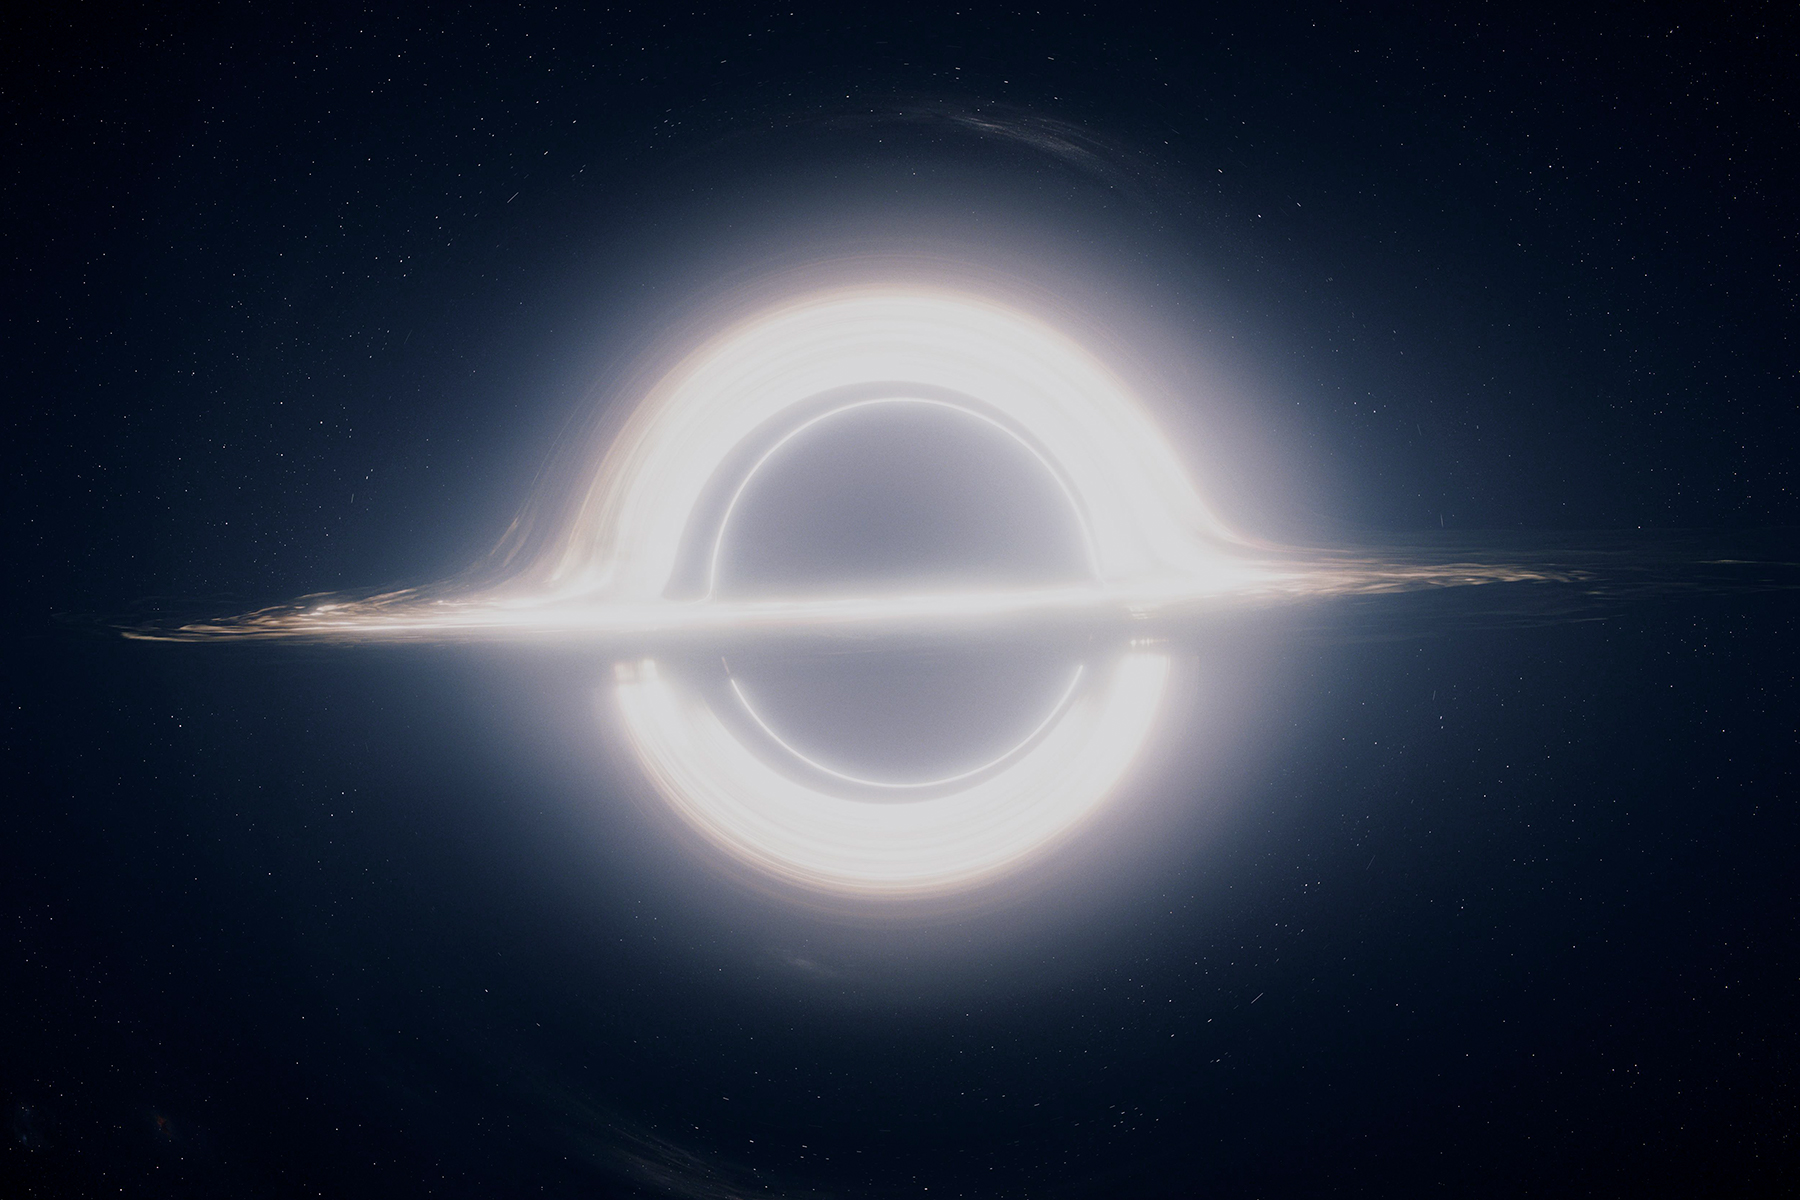
\includegraphics[width=.7\textwidth]{fig/chpt01/blackhole.jpg}
    \caption{\small 电影 \textit{Interstellar} 中黑洞 Gargantua 设定为一颗古老的巨型旋转黑洞,周围绕有的星尘称为\textbf{吸积盘}(accretion disk)。受引力作用,其间有高温物化反应,大量射线放出,包括可见光。观众看来,视界遮挡了部分光源,但光线仍可绕过视界,故视觉上吸积盘仿佛包裹了视界。}
\end{figure}
Wheeler 将视界半径超过其自身半径的星体称为\textbf{黑洞}(black hole)。目前已观测到这种星体。视界所包围的时空区域称为\textbf{黑洞区域},视界又可称黑洞表面。若星体斥力不能与引力抗衡,则质量将无限坍缩至 $r=0$,因而视界内极为空旷。

考虑到球对称性,只需研究 2 维 $\d s^2=-\left(1-{2M}/{r}\right)\,\text d t^2+\left(1-{2M}/{r}\right)^{-1}\text d r^2$。
用\textbf{类光测地线族}(family of null geodesics)研究时空的因果结构。
2 维图上每一点都可确定两条不同的类光测地线,所有类光测地线可分为两类。空间上朝外的称\textbf{外向}(outgoing),反之称\textbf{内向}(incoming)。
令 $\d s^2=0$,则
\eq{\label{dia_Sch}
t=\pm\left(r+2M\ln|r-2M|\right)+C.
}
考虑 $r>2M$,上式正负号取正后斜率为正,为外向族,负号对应内向族。然而 $r=2M$ 时 $t\to\infty$,故在 $\{t,x\}$ 系下任何物质永不落入视界。但请注意,同时的相对性导致“永远”的相对性。
考虑静止于 $r=r_0$ 的钟,其固有时满足 $\dv*{\tau}{t}={\sqrt{1-2M/r_0}}$。当 $r_0\to 2M$ 时 $\dv*{\tau}{t}\to 0$,说明在 Schwarzschild 系下,钟在视界处的读数 $\tau$ 近乎定格。
物理意义是,遥远观者需要通过对钟建立正交性,然而反射事件越接近视界,光就越难逃离,遥远观者接受光信号的用时就越来越久,对钟过程极为缓慢,从而出现永不落入的现象。
欲连续地描述粒子落入视界的过程,就是找到坐标系使测地线连续,也即消除度规的奇性。

考虑从 $r=r_0$ 释放的自由落体质点 $Z^\mu$。E-L 方程给出 $\dv{\tau}(g_{\mu\nu} Z^\nu)=\frac 12 g_{\alpha\beta,\mu} Z^\alpha Z^\beta$。由 $g_{\mu\nu,0}=0$ 知 $g_{0\nu} Z^\nu=\text{常数}$。取 $\nu=0$ 有 $Z^0=E/(1-{2M}/{r})$,其中 $E=1-2M/r_0$,因为 $r=r_0$ 时 $Z^0=1$。由模长归一性,并取内向有 $Z^1=-\sqrt{E^2-1+{2M}/{r}}$。对偶为 $Z_0=-1,Z_1=-(1-{2M}/{r})^{-1}{\sqrt{2M/r}}$。
下面按自由落体者建立新系 $\{\tau,R\}$。$\tau$ 可称\textbf{自由落体时}。由 $\tilde Z^\mu=\delta^\mu_0$ 知 $\tilde g_{0 0}=\tilde g_{\mu\nu}\tilde Z^\mu\tilde Z^\nu=-1$ 且对偶为 $\tilde Z_\mu = \tilde g_{\mu0}$。设 $\tilde g_{01} = 0$ 表示已对钟,则 $\tilde Z_0 = -1,\tilde Z_1 = 0$。代入 $\pdv{\tilde x^\mu}{x^\nu}\tilde Z_\mu=Z_\nu$ 得 $\pdv{\tau}{t}=-Z_0,\pdv{\tau}{r}=-Z_1$,即
\eq{
    \d\tau=\d t+\frac{\sqrt{2M/r}}{1-{2M}/{r}}\d r\implies \tau = t+2 \sqrt{2Mr}+2M\ln\abs{\frac{\sqrt{r}-\sqrt{2M}}{\sqrt{r}+\sqrt{2M}}}.
}
其中积分常数均取零。做 $t\to\tau$ 变换后有
\eq{\d s^2=-\left(1-\frac{2M}{r}\right)\d\tau^2+2\sqrt{\frac{2M}{r}}\d\tau\,\d r+\d r^2=-\d\tau^2+\left(\sqrt{\frac{2M}{r}}\d\tau+\d r\right)^2,}
这称为\textbf{Gullstrand–Painlevé 系},可以再加上没动过的 $r^2\d\Omega^2$。
分量收敛且 $g\ne 0$ 表明已消除了视界奇性,但还不满足 $\tilde g_{00}=-1,\tilde g_{01}=0$。
继续变换。
记 $\d R=A\d t+B\d r$,代入 $\tilde Z^1=\pdv{R}{x^\nu}Z^\nu$ 可知 $B=-A Z^0/Z^1$,则
$\d R=A\Big(\d t+\frac{\sqrt{r/2M}}{1-{2M}/{r}}\d r\Big)=A (\d\tau+\sqrt{r/2M}\d r)$,直接代入上述度规可知 $g_{11}=\frac{2M}{A^2r}$。
可见 $R$ 可确定到只差缩放函数 $A(t,r)$,因为各落体者间距任意。
不妨取 $A=1$,则 $R=\tau+\frac 23(2M)^{-1/2}r^{3/2}$。度规表为
\eq{
    \d s^2=-\d\tau^2+\frac{2M}{r}\d R^2+r^2\d\Omega^2,\quad r=(2M)^{1/3}\left(\frac 32(R-\tau)\right)^{2/3}.
}
这称为\textbf{Lemaître 系}。这是非稳态系,直观上,沿着落体运动 $R=R_0$ 当然感受到变化的引力场。
自由落体者在 $\tau=R$ 到达 $r=0$。这说明视界内时空极为空旷,且一旦进入视界便无法逃脱,最终落入奇点。

可见,显然


 则自然就

计算可得如下的\textbf{Kretschmann 标量}
\eq{
R_{\mu\nu\sigma\lambda}R^{\mu\nu\sigma\lambda} = \frac{48 M^2}{r^6},
}
上式在 $r=0$ 发散。这问题其实很严重,因为我们只是框定一堆物质,便使得光滑的时空上戳出一个“洞”,令人难以接受。$r=0,2M$ 两处的奇性在此体现出区别:上式在 $r=2M$ 有意义。
既然曲率在 $r=2M$ 处并不奇异,那就有可能找到坐标系使度规分量不发散。这种奇性称为\textbf{坐标奇性}或\textbf{假奇性},可尝试消除。
$r=0$ 的奇性就称\textbf{时空奇性}或\textbf{真奇性},因为曲率发散与坐标系无关。此点称\textbf{奇点}\footnote{英文亦是 singularity。为表述性质和地点两种概念,中文语境里可区分使用。但注意奇点不一定仅位于空间点。}。



并且,当视界内部很空旷时,对探险者而言,其进入视界时并无触觉,若稍有不慎,未能警觉自己所处位置,则很可能多走一步而遁入厄运。

当然,探险者还是能通过视觉上“眼前一黑”来观察,但更可怕的是,探险者并非真正的质点,而不同位置所受引力在此极端地带将差距巨大,因此潮汐力(对应于曲率大小)极有可能撕碎探险者,除非视界半径很大而稀释了曲率。此外,前文用测量效应说明了静态观者对探险者的观察,亦可用视觉效应这种现象。若静态观者借光信号观察探险者,则从图容易看出,随探险者逐渐接近视界,探险者所发出的光将越来越晚地到达静态观者,而坠入的画面无法传播出来。


\section{修改引力理论}
\subsection{宇宙学}
观测结果建议,宇宙在大尺度上\textbf{均匀}(homogeneous)且\textbf{各向同性}(isotropic)。这使得不能用非零质量密度和常数场强求解 Poisson 方程,因为在无限充斥的物质场中,试图计算某点场强时要涉及全空间体积分,而这种积分是反常的,其结果结果取决于有限域趋于无穷的方式。方式不同可得到“为零”或“发散”的结果。因此 Newton 引力论很难发展出宇宙学。

但广义相对论允许我们研究均匀各向同性的解及其扰动。
宇宙学的早期发展毫无疑问是 Einstein 带头。当时占统治地位的观点是静态宇宙。这使得 Einstein 为强行凑出静态解而修改场方程。注意除了选择 $R$,还可注意 $\sqrt{-g}\d[4]{x}$ 本身就已广义不变,故可考虑 $\mathcal L=\frac{1}{2\kappa}\left(R-2\Lambda\right)+\mathcal L_M$,结果是
\eq{
    R_{\mu\nu}-\frac12 g_{\mu\nu} R + \Lambda g_{\mu\nu}=\kappa T_{\mu\nu},
}
其中 $\Lambda$ 称为\textbf{宇宙学常数}(cosmological constant)。
根据具体的宇宙模型以及观测结果,可以确定其数值。
当然,在假设静态的情况下也能强行计算其值。但现代观点自 Hubble 开始普遍认为宇宙是\textbf{膨胀的}(expanding)。比如,\textbf{FLRW 解}就是膨胀宇宙的一阶近似。在膨胀模型下可不引入 $\Lambda$,故 Einstein 认为添加 $\Lambda$ 是其\textit{一生中所犯的最大错误}。1967 年 Hawking 证明了膨胀宇宙在时间上回溯可到达奇点,这被称为\textbf{宇宙大爆炸}(the big bang)。1990 年代的理论及观测显示,只有将 $\Lambda$ 重新写进来才能解释宇宙的\textbf{加速膨胀},其结果为 $\Lambda=1.1056\times 10^{-52}$\,m$^{-2}$。对通常的分析,这个数值太小,远不及 $\frac12 g_{\mu\nu} R$ 项的贡献,故会被忽略掉。
目前这一项被解释为\textbf{暗能量}(dark energy)的贡献。在量子场论中,能具备这一性质的概念只有真空能,然而两套理论给出的 $\Lambda$ 数值相差数量级很大。

还可考虑 $R_{\mu\nu} R^{\mu\nu},R_{\mu\nu\sigma\kappa}R^{\mu\nu\sigma\kappa}$ 等\textbf{Gauss-Bonnet 项}:
\eq{
    \mathcal L_G=\frac{1}{2\kappa}R+\alpha R_{\mu\nu} R^{\mu\nu}+\beta R^2+\gamma R_{\mu\nu\sigma\kappa}R^{\mu\nu\sigma\kappa}+\cdots,
}
甚至包括更高阶导数,其中耦合强度都是 $\hbar$ 量级的极小值。一般在日常尺度下可不考虑量子效应。

\subsection{Mach 原理及标量场}

Newton 为了解释绝对空间的存在性,提出了所谓的\textbf{水桶实验}。将一盛有清水的桶静置,并用一根长绳悬吊(图中略去)使桶可以靠绳索的扭力而转动;随后,尽可能使桶很快地加速旋转至某一角速度并保持。起初,桶相对于我们旋转,但(大部分)水由于惯性仍将保持静止,并且液面是平坦的;待桶的运动通过摩擦力传导至水,使水开始渐渐地随桶旋转,液面逐渐凹陷。在某个时刻,水和桶都将以该角速度旋转,即相对静止,液面凹陷呈抛物面状;尽可能很快地停止旋转,这个时候水由于惯性仍然要旋转一会儿才会静止,液面仍然凹陷。
虽说本质是思想实验,但其可行性还是挺大的:Newton 本人就声称“已经做过实验”,并对该结果表示肯定。
\begin{figure}[ht]\centering
    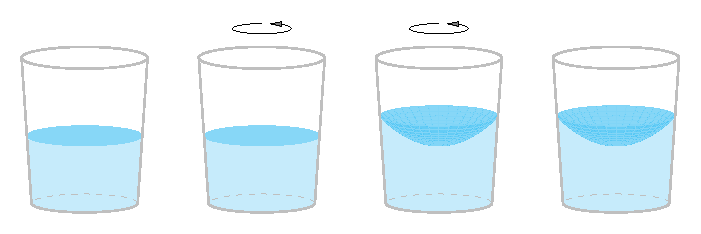
\includegraphics{fig/chpt01/spinning bucket.pdf}
    \caption{水桶实验}
\end{figure}
什么原因使液面凹陷?从经验中知道是水在相对于某个参考系旋转,进而产生了离心作用,但这个参考系是谁呢?起初水相对于环绕它的桶在旋转,随后水与桶一同旋转而相对静止的,但液面是凹陷的。因此,产生凹陷的旋转不是相对于水桶的旋转。Newton 认为这是相对于绝对空间的旋转。水面的凹陷是水的绝对运动的效果,通过凹陷程度可以测得其“绝对角速度”。Newton 认为如果水在其中旋转会凹陷,则这个参考系就是绝对空间。

19 世纪末,Mach 提出水并非相对于某种绝对介质旋转,而是相对于宇宙的全部物质组分,即星空背景。水凹陷是水的惯性效果,故 Mach 认为\textit{惯性需要在物质的相对运动中体现},或者\textit{物体惯性受到周围物质分布的影响}。这称为\textbf{Mach 原理},尽管是一条模糊的定性描述。准确地说,Mach 将桶参考系中所出现的惯性力理解为一种星空背景对水的作用,作用的强度体现为物体惯性,其大小与周围星空背景的质量及相对加速有关。比如,若周围物质很稀疏,就很难找到参照来判断一颗弹性球是否旋转,那么即使其旋转起来也不会形变。这似乎与引力很相似,但在实验上很难验证。因为反之需要加速周遭极大量的物质,绕着水桶旋转并观察水是否凹陷,尽管似乎直觉上应产生同样效果。

Einstein 也曾受到这一原理的启发,而去寻找惯性和引力的关系,最后抓住了等效原理。但实际上,等效原理给出的是新答案,即水是相对于局域惯性系运动。换言之,广义相对论已通过等效原理回答了这一问题。Einstein 起初以为广义相对论符合 Mach 原理,但现在看来显然不符合。且当代观点更多认为 Mach 原理至少在现有实验条件下是错误的。相反,等效原理受到支持的验证就多得多。若非要认为惯性起源于相互作用的话,由于局域惯性系是由外引力场决定的,因此可认为凹陷现象是水和引力场之间的互动造就的。目前用广义相对论回答“怎么办”是完全可行的,而“为什么”则是留给科学哲学。

1960 年代,Brans 和 Dicke\cite{Brans-Dicke} 提出了一个接近 Mach 原理愿景的引力理论。
首先注意,在地球的某个自由落体电梯中,等效原理的解释是电梯与乘客加速度一致,而 Mach 原理的解释是乘客的地球引力与星空背景的作用抵消。Newton 理论给出的地球引力为 $a=Gm/r^2$。假设星空背景有某种宇观质量 $M$ 和半径 $R$,并施加相同 $a$,根据量纲分析可知数量级上 $\frac{Gm}{r^2}\sim \frac{Rm}{Mr^2}$(几何制),因此 $\frac{1}{G}\sim\frac{M}{R}$。一种理解是 $\frac{M}{R}$ 由理论给出,而质量分布由广义相对论场方程的某个边界条件给出。还有一种是局部观察的 $G$(或场源质量)是随时空点变化的,其值由附近的质量分布决定。
假设 $G$ 是某个标量场的函数。首先想到 Ricci 标量,但它含有度规一阶导,随着与场源距离 $r$ 的增大,它比 $1/r$ 减小得还快。这种标量主要由附近质量分布决定,而非远处物质。因此,我们需要一个独立于度规以外的新标量场 $\phi$,但二者都用于描述引力场。假设理论是线性的,则前文表明乘客的惯性力贡献应是引力常数的倒数,即 $\phi\sim\frac{1}{G}$。
进而自由引力场加上标量场的部分为
\eq{
    \mathcal L_G=\frac{1}{16\pi} \left(\phi R-\frac{\omega(\phi)}{\phi}\partial_\mu \phi \partial^\mu \phi-2\Lambda(\phi)\right) ,
}
其中 $\omega$ 是耦合参数,$\frac{\omega}{\phi}$ 是为了使 $\omega$ 无量纲,并且还引入了$\Lambda(\phi)$ 代表可变的宇宙学常数。这就是\textbf{标量-张量理论}。准确地说,是
$\phi$ 的平均值 $\langle\phi\rangle$ 象征 $1/G$。

先对 $g^{\mu\nu}$ 变分,则
\begin{align*}
    16\pi \var(\mathcal L_G\sqrt{-g})&=\phi\left( G_{\mu\nu} \var g^{\mu\nu}+g^{\mu\nu}\var R_{\mu\nu}\right) \sqrt{-g}+ \Lambda g_{\mu\nu} \var g^{\mu\nu}\sqrt{-g}\\
&-\frac{\omega}{\phi}\left(\del_\mu\phi \del_\nu\phi-\frac 12 g_{\mu\nu}\partial_\lambda \phi \partial^\lambda\phi\right)\var g^{\mu\nu}\sqrt{-g},
\end{align*}
重点关注其中 $g^{\mu\nu}\var R_{\mu\nu}=2\nabla_\lambda(g^{\mu [\nu} \delta \Gamma_{\mu \nu}^{\lambda]})$。由于乘了 $\phi$,不能直接当做边界项丢掉,而要进一步用 $\var g^{\mu\nu}$ 表示克氏符变分。直接用协变导数 $\del_\mu g^{\sigma\lambda}+\Gamma^\sigma_{\mu\nu} g^{\nu\lambda}+\Gamma^\lambda_{\mu\nu} g^{\nu\sigma}=0$ 计算出克氏符。变分有 $\nabla_\mu \delta g^{\sigma\lambda}+g^{\nu\lambda}\delta \Gamma^\sigma_{\mu\nu} +g^{\nu\sigma}\delta \Gamma^\lambda_{\mu\nu} =0$。
用 $g^{\kappa\mu}$ 升指标,进行 $\kappa,\sigma,\lambda$ 轮换后加减消项,再缩并移项就有
\eq{
    \delta \Gamma_{\mu \nu}^\lambda=-\frac{1}{2}\left(g_{\kappa \mu} \nabla_\nu\delta g^{\kappa \lambda}+g_{\kappa \nu} \nabla_\mu\delta g^{\kappa \lambda}-g_{\mu \sigma} g_{\nu \kappa} \nabla^\lambda\delta g^{\sigma\kappa}\right).
}
进而与 $g^{\mu\nu}$ 缩并再取反称有
\eq{
    2g^{\mu [\nu} \delta \Gamma_{\mu \nu}^{\lambda]}=g_{\mu\nu}\nabla^\lambda \delta g^{\mu\nu} - \nabla_\mu\delta g^{\mu\lambda},
}
将该结果用于分部积分:
\begin{align*}
    2\int \phi \nabla_\lambda(g^{\mu [\nu} \delta \Gamma_{\mu \nu}^{\lambda]}) D^4x &\simeq -2\int  g^{\mu [\nu} \delta \Gamma_{\mu \nu}^{\lambda]} \nabla_\lambda \phi D^4x\\
    &= -\int  (g_{\mu\nu}\nabla^\lambda (\delta g^{\mu\nu})\nabla_\lambda \phi - \nabla_\mu(\delta g^{\mu\lambda}) \nabla_\lambda \phi)  D^4x\\
    &\simeq \int  (g_{\mu\nu} \delta g^{\mu\nu}\nabla^\lambda \nabla_\lambda \phi - \delta g^{\mu\lambda} \nabla_\mu\nabla_\lambda \phi)  D^4x\\
    &=\int  (g_{\mu\nu} \square_g \phi - \nabla_\mu\nabla_\nu \phi) \delta g^{\mu\nu} D^4x.
\end{align*}
故引入物质场后的结果为
\eq{
    \phi G_{\mu \nu}+\Lambda g_{\mu\nu}=8 \pi T_{\mu \nu}+\frac{\omega}{\phi}\left(\partial_\mu \phi \partial_\nu \phi-\frac{1}{2} g_{\mu \nu} \partial_\lambda \phi \partial^\lambda \phi\right)+\nabla_\mu \del_\nu \phi-g_{\mu \nu} \square_g \phi,
}
并注意其迹为
\eq{\label{eq:BDtrace}
    -R+4\frac{\Lambda}{\phi} =\frac{8 \pi}{\phi} T-\frac{\omega}{\phi^2}\partial_\lambda \phi \partial^\lambda \phi-\frac{3}{\phi}\square_g \phi.
}

再对 $\phi$ 变分:
\[16\pi\var(\mathcal L_G\sqrt{-g})= \left(\left(R-2\dv{\Lambda}{\phi}\right)\var\phi - \frac{1}{\phi}\del_\mu \phi \del^\mu \phi\dv{\omega}{\phi}\var\phi - \omega\var(\frac{1}{\phi}\del_\mu \phi \del^\mu \phi)\right) \sqrt{-g},\]
其中
\begin{align*}
    \int \var(\frac{1}{\phi}\del_\mu \phi \del^\mu \phi) D^4 x
    & =\int \left(-\frac{1}{\phi^2} \del_\mu \phi \del^\mu \phi \delta \phi+\frac{2}{\phi} \del^\mu \phi  \del_\mu \delta \phi\right) D^4 x \\
    & \simeq \int \left(-\frac{1}{\phi^2} \del_\mu \phi \del^\mu \phi \delta \phi-2 \nabla_\mu\left(\del^\mu \phi \frac{1}{\phi}\right) \delta \phi\right) D^4 x \\
    & =\int\left(-\frac{1}{\phi^2} \del_\mu \phi \del^\mu \phi \delta \phi-\frac{2}{\phi} \square_g \phi \delta \phi+\frac{2}{\phi^2} \del^\mu \phi \del_\mu \phi \var\phi\right) D^4 x\\
    & =\int\left(\frac{1}{\phi^2} \del_\mu \phi \del^\mu \phi  - \frac{2}{\phi} \square_g \phi \right)\delta \phi D^4 x.
\end{align*}
进而
\[
    R-2\dv{\Lambda}{\phi}-\frac{1}{\phi}\del_\mu \phi \del^\mu \phi\dv{\omega}{\phi}- \frac{\omega}{\phi^2} \del_\mu \phi \del^\mu \phi  + \frac{2\omega}{\phi} \square_g \phi=0.
\]
利用 \eqref{eq:BDtrace} 式替换掉 $R$ 可得
\eq{
    (3+2\omega) \square_g \phi+4\Lambda-2\phi\dv{\Lambda}{\phi}-\del_\mu \phi \del^\mu \phi\dv{\omega}{\phi}=8 \pi T.
}

具体地,考虑 $\dv*{\omega}{\phi}=0$ 和 $\Lambda=0$,则
\eq{
    \mathcal L_G=-\frac{1}{16\pi} \left(\phi R-\omega \phi^{-1} \partial_\mu \phi \partial^\mu \phi\right),
}
进而
\begin{gather}
    G_{\mu \nu}=\frac{8 \pi}{\phi} T_{\mu \nu}+\frac{\omega}{\phi^2}\left(\partial_\mu \phi \partial_\nu \phi-\frac{1}{2} g_{\mu \nu} \partial_\lambda \phi \partial^\lambda \phi\right)+\frac{1}{\phi}\left(\nabla_\mu \del_\nu \phi-g_{\mu \nu} \square_g \phi\right), \\
    \square_g\phi=\frac{8 \pi}{3+2 \omega} T.
\end{gather}
此即\textbf{Brans-Dicke 理论}。可见若 $\omega\to\infty$,则 $\phi$ 没有贡献,退回广义相对论。根据论文 \cite{Bhabra} 的结果,从 Schwarzschild 解的角度来看,对于非常大的 $\omega$,那么现有实验精度下,广义相对论和 Brans-Dicke 理论就已不可分辨。既然如此就选择广义相对论。截止到 2003年,飞往土星的 Cassini 飞船的 Doppler 跟踪(tracking)\cite{Will-thesis}的测量结果为 $\omega>40000$,即目前观测还是更倾向于广义相对论。

一个涉及宇宙暴胀的理论是 $f(R)$\textbf{理论},其中自由引力场的拉氏密度为 $\mathcal L_G=f(R)$。
记标量场 $f_R:=\dv*{f(R)}{R}$。变分有
\begin{align*}
\delta S_G &=  \int\left(f_R \delta R -\frac12 f(R) g_{\mu\nu}\delta g^{\mu\nu}\right) D^4x \\
&=  \int\bigg(f_R R_{\mu \nu} -\frac{1}{2} f(R) g_{\mu \nu} \bigg) \delta g^{\mu \nu}D^4x+2\int f_R \nabla_\lambda(g^{\mu [\nu} \delta \Gamma_{\mu \nu}^{\lambda]}) D^4x\\
&\simeq  \int\left(f_R R_{\mu \nu} -\frac{1}{2} f(R) g_{\mu \nu} +g_{\mu\nu} \square_g f_R - \nabla_\mu\nabla_\nu f_R\right) \delta g^{\mu\nu} D^4x,
\end{align*}
加上物质场的贡献有
\eq{
    f_R R_{\mu \nu}-\frac{1}{2} f(R) g_{\mu \nu}+g_{\mu \nu} \square_g f_R-\nabla_\mu \nabla_\nu f_R=\kappa T_{\mu\nu}.
}
可证 $f(R)$ 的作用实际上相当于引入额外标量场。我们以后再谈细节。

\subsection{Kaluza-Klein 理论}

我们甚至不排除更高维时空的存在,将四维时空中的相互作用视作更高维物理的结果。
Kaluza 最先注意到电磁张量看起来像截断克氏符:引入第五(空间)维度使得 $A_{\mu}=g_{\mu 4}$,假定 $g_{\mu\nu,4}=0$ 则
\eq{
    \Gamma^\mu_{\nu 4}=\frac{1}{2}g^{\mu\sigma}\left(2g_{4[\sigma,\nu]}+g_{\sigma\nu,4}\right)=-\frac{1}{2}F^\mu{}_{\nu}.
}
其中 $\mu,\nu$ 只取 $0,1,2,3$。假设五维“度规”形如
\eq{
    \d\hat s^2=\hat g_{ab}\d x^a\d x^b=g_{\mu\nu}\d x^\mu \d x^\nu+(\d x^4+\lambda A_\mu\d x^\mu)^2,
}
其中 $a,b$ 取 $0,1,2,3,4$。
也即
$\hat g_{\mu\nu}=g_{\mu\nu}+\lambda^2 A_{\mu}A_{\nu},\ \hat g_{\mu 4}=\lambda A_\mu,\ \hat g_{44}=1$。
这一“度规”显然对任意四维变换 $x'^\mu(x^\nu)$ 或平移 $x'^5=x^5+f(x^\nu)$ 不变,但对任意五维变换可变,故并非真正的五维流形上的度规。后者的结果正是规范变换 $A'_\mu=A_\mu-\del_\mu f$。
换言之,我们将 U(1) 对称性的内部自由度 $\theta$ 解释到了第五维 $x^4$。
依次计算克氏符、Ricci 张量和 Ricci 标量可得
\eq{
    \hat R=R-\frac{\lambda^2}{4}F_{\mu\nu}F^{\mu\nu}.
}
这意味着五维几何 $\hat{\mathcal L}=\hat R$ 可在四维时空下分化出引力和电磁作用,称为\textbf{Kaluza 奇迹}。为求五维度规行列式,只需先对角化。考虑
$H^\mu{}_{\nu}=\delta^\mu_\nu,\ H^4{}_{\nu}=-\lambda A_\nu,\ H^\mu{}_{4}=0,\ H^4{}_{4}=1$,
则 $\hat g_{\mu a} H^a{}_{\nu}=g_{\mu\nu},\ \hat g_{\mu a} H^a{}_{4}=\lambda A_\mu,\ \hat g_{4 a} H^a{}_{\nu}=0,\ \hat g_{4 a} H^a{}_{4}=1$。因此 $\hat g=g$。
但我们需要使对 $x^4$ 的积分收敛。注意 U(1) 变换中 $\theta$ 是周期等效的,因而第五维度对应于某个圆周。因而 U(1) 等效为了 SO(2)。这便是\textbf{紧化}(compactication)思想之源,最先由 Oskar Klein 引进。$g_{\mu\nu,4}=0$ 也称\textbf{圆柱条件}(cylindricity condition)。五维“时空”并非流形,在数学上是\textbf{纤维丛}(fiber bundle),四维时空作为其\textbf{底流形}而第五维圆圈作为其\textbf{纤维}。假设半径 $L$,则
\eq{
    \hat S=\frac{1}{16\pi\hat G}\int \hat R \sqrt{-\hat g} \d^5 x=\frac{L}{8\hat G}\int\hat R \sqrt{- g} \d^4 x,
}
Gauss 几何制下取 $\hat G=2\pi L,\lambda=2$ 即得真空 Einstein-Maxwell 作用量。再考虑五维测地线方程 $\ddot x^a+\Gamma^a_{bc}\dot x^b \dot x^c=0$。首先由圆柱条件知守恒量 $\pdv*{\mathcal L}{\dot x^4}\propto\dot x^4+A_\mu\dot x^\mu$。剩余分量为
\eq{
    \ddot x^\lambda+\Gamma^\mu_{bc}\dot x^b \dot x^c=\ddot x^\lambda+\Gamma^\lambda_{\mu\nu}\dot x^\mu \dot x^\nu-F^\lambda{}_\mu\dot x^\mu(\dot x^4+A_\nu\dot x^\nu)=0,
}
若用荷质比来确定守恒量,则这正是 Lorentz 力定律 $\dot x^4+A_\nu\dot x^\nu=q/m$。从而经典电磁力、经典引力得到统一。
带电粒子与中性粒子具有不同运动,这并不违反等效原理,而只是因为它们在 $x^4$ 上有不同初速度。

这一理论当然差强人意。$\hat R_{ab}=0$ 的真正结果为
\eq{
    F_{\mu\nu}F^{\mu\nu}=0,\quad \nabla_\mu F^{\mu\nu}=0,\quad R_{\mu\nu}=2 F_{\mu\sigma}F_{\nu}{}^{\sigma},
}
第三式只是真空 Einstein-Maxwell 方程 $R_{\mu\nu}=8\pi T_{\mu\nu}$ 在第一式成立的特例。第一式源于 $\hat R_{44}=0$。这是因为变分原理并不能保证 $\hat g_{44}=1$ 假设。从而,五维假设显得非常人为。最重要的是,我们始终在讨论经典理论,并未真正考虑量子力学。实际上,强、弱相互作用的概念在 Einstein 逝世后才被彻底确立。

此外还必须解释为何从未发现第五维度。置五维闵氏时空上的复标量场 $\hat\phi$。方便起见考虑无质量,Klein-Gordon 方程为
\eq{
    \hat\eta^{ab}\del_a\del_b\hat\phi=0,\quad \hat\phi=\sum_n\phi_n(x^\mu)\e^{\i n x^4/L},
}
其中由周期性 $x^4\sim x^4+2\pi L$,可对 $\hat\phi$ 作 Fourier 展开使其与 $x^4$ 的依赖关系更明确。代入展开式得到无穷多个解耦方程,即对 $\hat\phi$ 的无穷多 Fourier 模 $\phi_n$ 均有
\eq{
    (\square-m_n^2)\phi_n^2=0,\quad m_n^2={n^2}/{L^2}.
}
其中质量项源于 $\del_{44}$。可见五维时空上的无质量标量场会产生 $n=0$ 的四维无质量场\footnote{但仍有 d'Alembert 方程,故内部空间是谐振的或振动模固定。}、$n\ne 0$ 的无穷多有质量场。这种质量称为 Kaluza-Klein 模。

四维闵氏度规在五维上的拓展其实应为 $\d\hat s^2=\eta_{\mu\nu}\d x^\mu \d x^\nu+(\d x^4+\lambda A_\mu\d x^\mu)^2$,则 $\hat g=g=-1$。因此 $\hat g^{\mu\nu}=\eta^{\mu\nu},\hat g^{\mu 4}=-\lambda A^\mu,\hat g^{44}=1+\lambda^2 A^\mu A_\mu$。
Klein-Gordon 方程变为
\[
    0=\square_{\hat g}\hat\phi=\del_a\left(\hat g^{ab}\del_b \hat\phi\right)=\eta^{\mu\nu}(\del_\mu-\lambda A_\mu\del_4)(\del_\nu-\lambda A_\nu\del_4)\hat\phi+\del_4^2\hat\phi,
\]
将 Fourier 分解代入,则对任意 $\phi_n$ 有
\[
    \left(\eta^{\mu\nu}\left(\del_\mu-\i\frac{\lambda_n}{L} A_\mu\right)\left(\del_\nu-\i\frac{\lambda_n}{L} A_\nu\right)-m_n^2\right)\phi_n=0,
\]
可见非零模不仅有质量,且在规范场 $A_\mu$ 下带电。$\del_\mu-\lambda m_n A_\mu$ 与规范协变导数 $\del_\mu-\i ne A_\mu$ 对比得元电荷 $e=\lambda/L$。还原国际单位有 $e=\hbar\lambda/L$,以及 $\frac{c^4}{16\pi G}R-\frac{1}{4\mu_0}$。

$\nabla^\mu\phi\nabla_\mu\phi$ 代替即可,因而算子 $\square$ 换为 $\square_g$。

时空各点的额外维蜷缩(curled up),从而只剩下我们经验中看到的时空本身。

尽管有诸多缺陷,Wheeler 仍表示“几何动力学”拓展到其它相互作用是有希望的。20 世纪末,\textbf{弦论}(string theory)继承了高维几何的衣钵,利用极小对象“弦”部分地得到了广义相对论、量子场论的结果。此外还有企图构建背景无关量子场论的\textbf{圈量子引力}(loop quantum gravity)、研究非交换几何的\textbf{CLCB 理论},它们皆只部分地回答了量子引力的疑难。目前前沿话题还包括引力同统计物理、信息论的联系,诸如\textbf{熵力理论}、\textbf{黑洞信息学},以及受场论和凝聚态影响的\textbf{超对称理论}。
我们以后再详细学习。

引力是目前已知相互作用中最弱的。两个质子之间的静电斥力比它们之间的引力大 $1.2 \times 10^{36}$ 倍。这意味着即使各种量子引力理论层出不穷,但以当代技术,仍然很难直接做实验以获取有效数据。目前多用宇宙学观测所得到早期宇宙的数据来筛选理论。“大一统理论”通常指沿标准模型的思路,将强相互作用同电弱作用统一的尝试。狭义上的量子引力理论只涉足引力量子化问题,广义的量子引力理论或许是人们所希望的“万物理论”。

\section{标架表述}

还可考虑有挠时空,$g_{\mu\nu},T^\lambda{}_{\mu\nu}$ 一齐作为引力场的基本物理量。这种理论发展为\textbf{引力规范理论},典型地如\textbf{Einstein-Cartan 理论}。这些理论多采用了更为数学、但实质等价于 $g_{\mu\nu},T^\lambda{}_{\mu\nu}$ 形式的语言,故暂时只扼要介绍。其中 2 阶情形的最一般的规范理论作用量为
\eq{
\begin{aligned}
\mathcal L_G= & -\frac{1}{2\kappa}(R-2 \Lambda)+a_1 R_{\alpha \beta \mu \nu} R^{\alpha \beta \mu \nu}+a_2 R_{\alpha \beta \mu \nu} R^{\mu \nu \alpha \beta} \\
& +a_3 R_{\alpha \beta \mu \nu} R^{\alpha \mu \beta \nu}+b_1 R_{\alpha \beta} R^{\alpha \beta}+b_2 R_{\alpha \beta} R^{\beta \alpha} \\
& +c_1 T_{\alpha \beta \gamma} T^{\alpha \beta \gamma}+c_2 T_{\alpha \beta \gamma} T^{\beta \gamma \alpha}+c_3 T^\beta{}_{\alpha \beta} T_\gamma{}^{\gamma \alpha}.
\end{aligned}
}
其中 $R_{\alpha \beta \mu \nu}$ 是一般的\textbf{有挠 Riemann 曲率},前一对指标与后一对指标没有对称性,前一对指标也没有反称性。但 Ricci 张量仍按 $R_{\alpha \beta}=R^\mu{ }_{\alpha \mu \beta}$ 定义。其中的指标升降均在 $g_{\mu\nu}$ 下。

\section{哈氏理论}
\subsection{3+1 分解}

\subsection{初值问题}

\section{场论 Noether 定理}\label{sec:Noether}

   % 广义相对论
    \chapter{黑洞物理}\label{chpt:BH}

\section{经典实验验证}

黑洞是广义相对论提出之后,第一个也是最重要的研究课题。百年来围绕着黑洞的研究,使我们对相对论、引力、量子场论、统计物理都有了崭新的认识。
而自 Einstein 论文发表以来,对广义相对论的若干实验验证相继提出,其中最为著名的是引力红移、水星进动和星光偏折。

\subsection{引力红移}



考虑等效原理。

假设有一光源在 $r$ 处发出频率为 $\nu$ 的光子,若此时光源静止于某惯性系,则光子能量为 $E=h\nu$。若此时光源以速度 $v$ 沿径向运动,则能量变为
\[E'=h\nu\sqrt{1-v^2/c^2}.\]
若光子在 $r$ 处被接收,且接收器静止于同一惯性系,则光子能量仍为 $E=h\nu$。因此,光子在 $r$ 处的频率为
\[\nu'=\frac{E'}{h}= \nu\sqrt{1-v^2/c^2}.\]
若光源和接收器处于不同的引力场中,设光源在 $r_1$ 处,接收器在 $r_2$ 处,则光子能量为
\[E=h\nu\sqrt{1-2GM/r_1c^2},\]
接收器处的能量为
\[E'=h\nu\sqrt{1-2GM/r_2c^2}.\]
因此,光子在 $r_2$ 处的频率为
\[\nu'=\frac{E'}{h}= \nu\sqrt{\frac{1-2GM/r_2c^2}{1-2GM/r_1c^2}}.\]
这就是引力红移的公式。若 $r_1=r_2$,则 $\nu'=\nu$,即光子频率不变;若 $r_1<r_2$,则 $\nu'<\nu$,即光子频率降低;若 $r_1>r_2$,则 $\nu'>\nu$,即光子频率升高。

引力红移的实验验证是通过测量光子频率的变化来实现的。最著名的实验是 Pound-Rebka 实验,该实验在 1959 年由 Robert Pound 和 Glen A. Rebka 在哈佛大学进行。他们使用了一个高塔和一个伽马射线源,测量了从塔顶到塔底的伽马射线频率变化,验证了引力红移的预测。

\subsection{水星进动}

\begin{wrapfigure}{r}{3cm}\centering
    \begin{tikzpicture}[scale=.5]
    \draw[domain=0.4*180/pi:21.6*180/pi,samples=300] plot ({cos(\x)/(1-0.5*cos(0.97*(\x-45)))},{sin(\x)/(1-0.5*cos(0.97*(\x-45)))});
    \fill (0,0) circle(3pt);
    \end{tikzpicture}
    \caption{\small 轨道进动(离心率和进动角均夸大)}
\end{wrapfigure}

19 世纪末,水星近日点进动现象被首次观测。毫无干扰的情况下,Newton 理论当然不能解释进动,因此必须要考虑其它因素,如同当年从天王星轨道扰动发现的“笔尖下的行星”海王星那样。由于地球自转轴的进动,从地球上观测水星的进动大部分是参考系的视觉效果,即岁差,我们直接扣除它。其它因素就是其余行星造成的摄动、太阳实际形状以及广义相对论相应。

先研究摄动。参见 Goldstein《经典力学》第 5$\sim$8 章。
以太阳为参考,水星所处的外引力场写作
\[\bm F(r,t)=\bm F_\odot+\bm F_p=-\frac{{G{M_\odot}m}}{r^3}\bm r-Gm\sum_i\frac{M_i(\bm r-\bm R_i)}{|\bm r-\bm R_i|^3},\]
前一项是太阳的贡献,后面是各行星的作用总和。现在研究后者。设 $\bm r,\bm R_i$ 夹角 $\theta_i$,则 $d_i=|\bm r-\bm R_i|=R_i^2(t)+r^2-2R_i(t)r\cos\theta_i(t)$。
忽略其余行星轨道的离心率之影响,即假定做半径 $\bm R_i$ 的圆周运动。设单个行星角速度为 $\omega_i$,将 $\bm F_p$ 在时域上做 Fourier 展开
\[
\bm F_p=- Gm\sum_i \sum_{n\in\Z} {{a_n}(r){\e^{\i n{\omega_i}t}}}\frac{\bm r-\bm R_i}{|\bm r-\bm R_i|},\quad a_n=\frac{\omega_i}{2\pi}\int_0^{2\pi/\omega_i}{\frac{{M_i\e^{-\i n\omega_i t}\,\d t}}{{R_i^2 + r^2 - 2R_ir\cos \theta_i}}}.
\]
只保留最低阶的 $n=0$ 并用$\d\theta_i$ 替换$\omega_i\d t$ 就可使引力势同时间无关,得到近似表达
\eq{\bm F_p(r) = - Gm\sum_i  \int_0^{2\pi } \frac{M_i\,\d\theta/2\pi}{R_i^2 + r^2 - 2{R_i}r\cos \theta  }\frac{\bm r-\bm R_i}{|\bm r-\bm R_i|},}
引入线密度 $\lambda_i=M_i/(2\pi R_i)$,并沿水星初始方向为极轴,在黄道面上建立极坐标系 $(r,\theta)$,便发现上式表明,其余行星对水星的作用相当于 $M_i$ 均匀分布的一个圆环。这符合直觉,毕竟水星的进动极为缓慢,完整进动一周所需时间相较于其它行星周期很长,因此其它行星的作用的确和圆环类似。但对离水星较近的行星(比如金星),二者周期将在同一数量级,因此不便于近似为圆环。可见圆环模型成立条件是 $R_i\gg r$。幸好,除金星外其它行星都离得较远,将金星视作圆环的影响并不致命。问题现在相当于,在太阳引力基础上,计算附加这样一个微扰后行星的进动。
由圆环对称性,可知作用力与 $\bm r$ 同向,即
\[
\bm F_p= Gm\frac{\bm r}{r}\sum_i  \lambda_iR_i\int_0^{2\pi } \frac{\cos\alpha\,\d\theta}{ d_i^2},
\]
可见其他引力的作用可视作朝外的有心力,我们就可直接讨论分量 $F=F_\odot+F_p$。
我们希望先计算出 $F_p$ 与 $r$ 的关系,虽无初等表达,但由于该式本身就具条件 $R_i\gg r$,故可近似计算。一个聪明的做法并非按 $r/R_i$ 展开,而是重构模型本身。将 $(r,\theta)$ 平移以使原点与水星重合,记新坐标 $(d,\alpha)$,则 $R_i^2=r^2+d_i^2+2rd_i\cos\alpha$,
由于 $\alpha=0$ 时 $d_i=R_i-r$,取解 $d_i=-r\cos\alpha+\sqrt{R_i^2-r^2\sin^2\alpha}$。
由 $R_i\gg r$ 知圆环可近似看作按 $\alpha$ 均匀分布,故 $ R_i\d\theta\approx d_i\d\alpha$,于是
\begin{align*}
    \int_0^{2\pi } \frac{R_i\cos\alpha\,\d\theta}{ d_i^2 }&\approx \int_0^{2\pi } \frac{\cos\alpha\d{\alpha}}{-r\cos\alpha+\sqrt{R_i^2-r^2\sin^2\alpha}}\\
    &=\int_0^{\pi } \left(\frac{\cos\alpha\d{\alpha}}{-r\cos\alpha+\sqrt{R_i^2-r^2\sin^2\alpha}}-\frac{\cos\alpha\d{\alpha}}{r\cos\alpha+\sqrt{R_i^2-r^2\sin^2\alpha}}\right)\\
    &=\frac{2r}{R_i^2-r^2} \int_0^{\pi }\cos^2\alpha\d{\alpha}=\frac{\pi r}{R_i^2-r^2},
\end{align*}
即
\eq{
F_p=Gm\pi r\sum_i \frac{\lambda_i}{R_i^2-r^2}.
}

接下来只以初始位置 $(r_0,0)$ 为极轴方向建立极坐标,以研究水星运动。有心力的形式为
$m(\ddot r-\dot\theta^2r)=F(r), 2\dot r\dot\theta+\ddot\theta r=0$。第二式导致角动量守恒,记 $mr^2{\dot \theta}=L$。在力学课学过如何从两式消 $t$ 得 Binet 式
\eq{
\dv[2]{\mu}{\theta}+\mu=-\frac{mF}{L^2\mu^2}=J(\mu),\quad \mu=1/r.
}
默认加入微扰前是圆轨道模型,则 $\dv*{\mu}{\theta}=0,F_0=-{L^2}/{(mr_0^3)}$,从而 $\mu_0=J(\mu_0)$。
然而圆轨道闭合而不一定稳定。稳定即是说,物体运动受到微扰后依然束缚在圆轨道附近。下面寻找稳定条件。在 $\mu_0$ 附近展开 $J(\mu)$,记 $x=\mu-\mu_0$,只保留至一阶可得波动方程
\[
\dv[2]{x}{\theta}+\left(1-\eval{\dv{J}{x}}_{0}\right)x=0.
\]
如果括号为负,$x$ 将随 $\theta$ 指数增长或衰减,显然不再稳定。因此稳定要求括号为正,则 $x$ 将随 $\theta$ 作周期振荡。代入 $J(\mu)$ 定义得
\[\eval{\dv{J}{x}}_{0}=\eval{\dv{\mu}}_{\mu_0}\left(- \frac{mF}{L^2\mu^2} \right)= \frac{2m}{L^2\mu_0^3}F_0 - \frac{m}{L^2\mu_0^2} \eval{\dv{F}{\mu}}_{\mu_0} = -2 - \frac{r_0}{F_0} F'(r_0).\]
这里撇号表示对 $r$ 求导。则稳定轨道要求有心力的形式满足
\eq{
1-\eval{\dv{J}{x}}_{0}=3+\frac{r_0}{F_0} F'(r_0)>0.
}
在波动方程中,这个括号的含义是频率平方,注意其中是对 $\theta$ 求导而非 $t$,故应是
\[
\frac{2\pi}{\Delta\theta}=\sqrt{3+\frac{r_0}{F_0} F'(r_0)}.
\]
其中 $\Delta\theta$ 的含义就是一次微扰振荡周期
\[
T_r=\frac{\Delta\theta}{\dot\theta}=\frac{\Delta\theta mr_0^2}{L}=\Delta\theta\sqrt{-\frac{F_0}{mr_0}}
\]
所扫过的角度。可见只有 $F_\odot$ 时使 $\Delta\theta=2\pi$,相当于又回到原位而无进动。而一旦错开,一次周期内就出现了进动。代入数据知
\eq{
r_0F_p'(r_0)=Gm\pi r_0 \sum_{i=2}^9 \lambda_i\frac{R_i^2+r_0^2}{(R_i^2-r_0^2)^2}\approx 1.088 \times 10^{16}\,\mathrm{N},
}
而 $F_p(r_0)\approx 7.587 \times 10^{15}\,\mathrm{N}, F_\odot(r_0)\approx -1.318 \times 10^{22}\,\mathrm{N}$。代入 $F=F_{\odot}+F_p$ 于 $\Delta\theta$ 则\footnote{为更便于计算,还可注意 $F_p(r_0)\approx r_0 F_p^{\prime}(r_0) \ll |F_\odot(r_0)|$,则展至 $F_p(r_0) / F_\odot(r_0)$ 和 $F_p^{\prime}(r_0) / F_\odot(r_0)$ 的一阶。}
\eq{
\Delta \theta=2\pi\sqrt{\frac{F_{\odot}(r_0)+F_p(r_0)}{F_\odot(r_0)+3F_p(r_0)+r_0F_p'(r_0)}}\approx 2\pi(1+9.884\times 10^{-7}).
}
进动率为
\eq{
\omega=\frac{\Delta\theta-2\pi}{T},
}
式中 $T$ 为水星公转周期,一般取恒星年(sidereal year)\footnote{某行星的恒星年是太阳在黄道上的视位置相对遥远恒星变化一周所经历时间,也相当于该行星相对于遥远恒星公转一周所经历的时间。千禧年时地球恒星年的平均长度为 365.25636 天。回归年(tropical year)是太阳的平黄经变化一周所经历时间。由于太阳视运动非均匀,选取不同的起点会得到不同的长度。若选取春分点作为基准,太阳从春分点出发运行一周再次回到春分点的时间为春分点年。千禧年时回归年的平均长度为 365.24219 天。恒星年比回归年要长 20 分 24.5 秒,这个差异正是地球造成的岁差。},或甚至是 $T_r$,再不济用 Kepler 第二定律计算亦可。代入数据知
\[\omega\approx\frac{\pi(1.977\times 10^{-6})}{87.969\,\text{天}}\approx 532''/\text{世纪},\]
仍与观测值 $575''$/世纪相差 $43''$/世纪。

再考虑广义相对论效应。

通过求解在所谓的\textit{线性近似}下的场方程,就可以算出水星近日点进动的正确值。只要能够取得这个进动的正确值,就表示广义相对论的正确性已经通过了该实验的检验。



\subsection{星光偏折}
Eddington(1882-1944,英国天体物理学家) 在 1919 年的一次日食观测中摄下了光线被引力“弯曲”的图片。这一点已经在几何光学近似中从理论上计算过。从那以后,用太阳系的种种检验对场方程作了所谓的,这些预测和实验都在这个物理条件下以很高的精度证实了广义相对论.

如果我们考虑黑洞附近的光线,一路走向测地线方程,所描述的轨迹曲线可以作为\textit{引力透镜(gravitational lensing)}的定量解释。

\subsection{后 Newton 理论}

(post-Newtonian theory)

\section{时空延拓}

\subsection{Eddington 系}

注意到内向族分别在 $r>2M,0<r<2M$ 单调,可设想直接将其映射为向内 $45^\circ$ 斜率的直线 $\tilde t=-r+C$,且为了 $r=0$ 时 $t=\tilde t$,可取
\eq{
    \tilde t=t+2M\ln\abs{\frac{r}{2M}-1}.
}
则度规表为
\eq{
\d s^2=-\left(1-\frac{2 M}{r}\right) {\d \tilde t}^2+\frac{4M}{r}\,\mathrm{d} \tilde t\, \mathrm{d} r+\left(1+\frac{2 M}{r}\right)\d r^2,
}
$g_{01}\geqslant 0$ 符合黑洞演化的方向。现在度规分量在视界处收敛,且 $g=-(g_{01})^2\ne 0$,这才算消去奇性。


$t=-r_*+C$,且为了 $r=0$ 时 $r_*=0$,可取
\eq{
    r_*=r+2M\ln\abs{\frac{r}{2M}-1}.
}
类比 Zeno 悖论\footnote{古希腊哲学家 Zeno 描述了类似效应:运动员 Achilles 欲同一只乌龟赛跑,且乌龟起点先于他若干路程 $L$。按通常的时间 $t$ 来说,他的速度 $v_1$ 快于乌龟的 $v_2$,明显在有限时间 $t=L/(v_1-v_2)$ 内超过乌龟。但设想这样计时:他欲超过乌龟,必须先追至乌龟的起点,但一旦如此,乌龟又能前进若干步,这样便有新的起点等着他,如此这般有无穷多这样的起点,则他“永远”也赶不上乌龟。这种计时方法称为 Achilles 时或 Zeno 时,记作 $t'$。令 $t',t$ 皆起于零。当 $t=L/v_1$ 时,Achilles 到达乌龟在 $t'=0$ 时的起点, $t'$ 加一,以此类推有
\[t=\sum_{i=0}^{t'-1} \frac{L}{v_1}\left(\frac{v_2}{v_1}\right)^{i}=\frac{L}{v_1-v_2}\bigg(1-\bigg(\frac{v_2}{v_1}\bigg)^{t'}\bigg)\implies t'=\frac{1}{\ln(v_2/v_1)}\ln\left(1-\frac{v_2-v_1}{L}t\right),\]
其中将 $t'\in\N$ 自然延拓至 $t'\in\R_+$。可见 $t'$ 在 $t=L/(v_2-v_1)$ 发散,因此按 $t'$ 衡量他永不超过乌龟。},
可称\textbf{乌龟坐标}(tortoise coordinates)。数学中的 Lambert 函数定义为满足 $x=y\e^y,y\geqslant -1$ 的$y=\operatorname{W}(x)$。用它可解出 $r=2M(1+\operatorname{W}(\pm\e^{r_*/2M-1}))$,正负号对应 $\sgn(r-2M)$。
注意 $\d r_*={\d r}/{(1-2M/r)}$,从而度规表为 $\d s^2=(1-2M/r)\left(-\d t^2+\d r_*^2\right)$,奇性消除了。关键在于,新坐标系给视界赋予发散坐标,就可将度规奇性隐藏起来。

但这个变换还不够,因为行列式 $g$ 在 $r=2M$ 为零。

时间也需要变换。

变换 $x'=x+(r_*-r)$ 在 $r<2M$ 时 $x'<x$,故称\textbf{超前}(advanced)变换,而 $x'=x-(r_*-r)$在 $r<2M$ 时 $x'>x$,故称\textbf{推迟}(retarded)变换。

该坐标系称为\textbf{超前 Eddington–Finkelstein 系},简称 Eddington 系。



利用十字相乘法可分解出两个类光测地线族,其一是
\eq{
\dv{\tilde t}{r}=\frac{r+2M}{r-2M}\Rightarrow \tilde t=r+4M\ln\abs{r-2M}+C_1, \quad r=2M,
}
其二是
\eq{
\dv{\tilde t}{r}=-1\Rightarrow \tilde t=-r+C_2.
}
显然前者为外向族而后者为内向族。
\begin{figure}[h!]
    \centering
    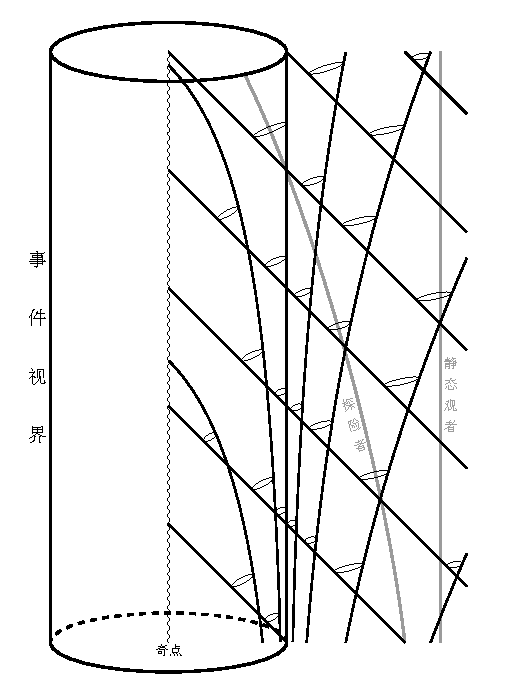
\includegraphics[width=.6\textwidth]{fig/chpt02/schBH.pdf}
    \caption{\small 静态黑洞 Eddington 图。绘制时积分常数均匀选取。可在格处画上椭圆,构成“妙脆角”,以代表微小未来光锥,或用“沙漏”表示完整光锥。}
\end{figure}
其中设有一个静态观者和一个位于 $\tilde t$-$r$ 平面的探险者。

\subsection{Kruskal 系}
Schwarzschild 系能保证 $g_{01}=0$ 而 Eddington 系不然。是否存在一个坐标系既能消除奇性,又能保持 $g_{01}=0$?

双曲线的渐近线相当于原点处的光锥 $C_N$。故对匀加速观者而言,信息不能从光锥另一侧逾越过来

故称\textbf{Rindler 视界}。

同理求出内、外向族分别为
\[
t=-\ln x+C_1,\quad t=\ln x+C_2.
\]
故可绘制如下图 。

注意,闵氏度规在 Rindler 系是有奇性的,因为其行列式 $g=-x^2$ 在 $x=0$ 处为零。可见,Rindler 系和闵氏系的相对地位,就像是 Schwarzschild 系或 Eddington 系和“更好”坐标系的相对地位。



因此上述类光测地线族其实“对应于”闵氏时空里的类光测地线族
\[
T=-X+C_1,\quad T=X+C_2.
\]

仿照这一思想,欲视类光测地线族为坐标网格(称为\textit{类光坐标})。

第  节中将双曲线、射线视作坐标线而衍生出 Rindler 坐标系,在 Rindler 图  里,这是在令
\eq{
v=t+\ln x,\quad u=t-\ln x.
}
度规表为 $\d s^2=-\e^{v-u}\d v\d u$。

而在闵氏图里是令
\eq{
V=T+X,\quad U=T-X,
}
或
\eq{
T=\frac{V+U}{2},\quad X=\frac{V-U}{2},
}
这有双曲函数的形式,而 $T,X$ 与 $t,x$ 的变换正是双曲函数,

故易知如下指数式
\eq{
V=\e^v>0,\quad U=-\e^{-u}<0.
}
度规现表为 $\d s^2=-\d V\d U$,不存在任何坐标奇性。

\begin{figure}[h!]
    \centering
    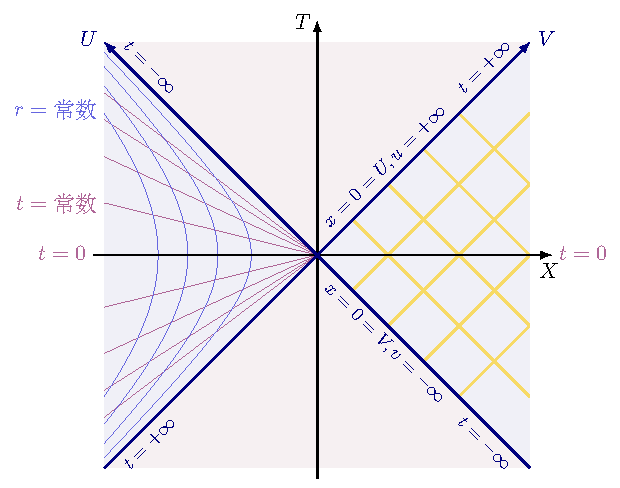
\includegraphics[width=.6\textwidth]{fig/chpt02/rindler.pdf}
    \caption{消除 Rindler 系的坐标奇性}
    \label{fig:rindlerIM}
\end{figure}
如图 \ref{fig:rindlerIM} 所示,则从直观上,闵氏时空图就像是把 Rindler 图 里竖直的 $x=0$ 从 $t=0$ 处向右“掰弯”成如光锥面一般的 Rindler 视界 $T^2=X^2$,即 $VU=0$,由上式知 $V,U$ 轴正方向如图 \ref{fig:rindlerIM}。图中蓝色双曲线代表等 $r$ 线,红色射线代表等 $t$ 线。可见,从 Rindler 图到闵氏图经历了如下过程:
\[
(t,x)\to(v,u)\to(V,U)\to(T,X).
\]
依葫芦画瓢地寻找“更好”坐标系。在超前 Eddington 系中,时间对角项在 $r=2M$ 为零,为消除奇性,只能借由超前变换所产生的非零时空交叉项,但我们并不想要交叉项。可见,必须使 $T,X$ 坐标的时间对角项非零。回到 Schwarzschild 系。不妨先研究 $r>2M$。$v,u$ 从类光测地线族产生,注意式 \eqref{dia_Sch} 与 $t=\pm r_*$ 相差常数,因此内、外向族分别给出
\eq{
v=t+r_*,\quad u=t-r_*.
}
由于 $r_*$ 作了超前变换,因此前者称\textit{超前类光坐标},后者称\textit{推迟类光坐标}。可见对 Rindler 时空来说其乌龟坐标是 $x_*=\ln x$,读者很容易验证这一点。度规在 $v,u$ 下表为
\[
\d s^2=-(1-2M/r)\d v\d u,
\]
沿用 $V,U$ 的指数形式但预留待定常数(只可与 $M$ 有关)以使最终的时间对角项非零\footnote{有种做法是填上 $1/\beta=4M$ 因子以约去指数求导出的系数,这样度规 \eqref{eq:kruskal} 中 ${32M^3}/{r}$ 变为 $2M/r$。}:
\eq{
V=\e^{\beta v}>0,\quad U=-\e^{-\beta u}<0.
}
只预留一个是考虑到对称性。进而度规表为
\[
\d s^2=-\beta^{-2} (1-2M/r) \e^{\beta(u-v)} \d V\d U,
\]
考虑到 $T,X$ 系只是 $V,U$ 系的旋转,我们可将其定义沿用至此,则 $-\d V\d U=-\d T^2+\d X^2$,进而保证无交叉项。现在的目标就是约掉 $(1-2M/r)$ 通分后所含因子 $(r-2M)$。这份任务只能交由 $\e^{\beta(u-v)}$,我们就要用 $r$ 表示它(由稳态条件可预料无 $t$)。注意 $u-v=-2r_*$,代入 $r_*$ 定义有
\[
\e^{\beta(u-v)}=\e^{-2\beta r}\left(\frac{2M}{r-2M}\right)^{4\beta M},
\]
说明应取 $\beta=1/4M$,则
\[
\d s^2=-\frac{32M^3}{r}\e^{-r/2M}\d V\d U=\frac{32M^3}{r}\e^{-r/2M}(-\d T^2+\d X^2).
\]
这里仍留有一个不能消除的时空奇点 $r=0$,与 Rindler 情况有所不同。综上,还原另外两个空间维度后,Schwarzschild 度规就表为
\eq{\label{eq:kruskal}
\d s^2=\frac{32M^3}{r}\e^{-r/2M}(-\d T^2+\d X^2)+r^2\d\Omega^2,
}
这里 $r$ 视作 $T,X$ 的函数,易知
\eq{
X^2-T^2=-VU=\e^{(v-u)/4M}=\left(\frac{r}{2M}-1\right)\e^{r/2M},
}
可用 Lambert 函数将其表为
\eq{\label{eq:r=T,X}
r=2M\operatorname{W}\left(\frac{X^2-T^2}{\e}\right)+2M.
}
这个坐标系称为 \textit{Kruskal 系}。我们再次按 $T,X$ 正交绘制 2 维时空图。$(-\d T^2+\d X^2)$ 形式的保留使类光测地线斜率仍为 $\pm 1$。实际上,像这样给原度规乘以一个正因子就称为 \textit{Weyl 重标度(rescaling)变换},简称 Weyl 变换,它能保留时空结构,故又称为\textit{共形(conformal)变换}。
\begin{figure}[h!]
    \centering
    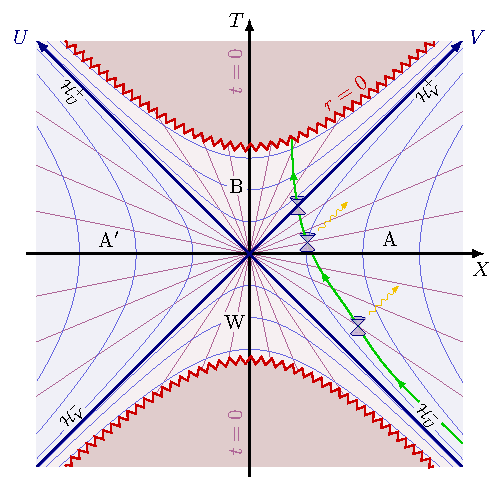
\includegraphics[width=.6\textwidth]{fig/chpt02/kruskal.pdf}
    \caption{Kruskal 延拓}
    \label{fig:kruskal}
\end{figure}
从图 \ref{fig:kruskal} 上可见,Kruskal 系也会“掰弯” Schwarzschild 时空的视界 $r=2M$,使之变为光锥面 $VU=0$。易知各坐标的取值分布同图 \ref{fig:rindlerIM} 相似。然而,我们只考虑了 $r>2M$ 的情况,在图上标记为开区域 \textit{A 区},对应 $V>0,U<0$。那 $r<2M$ 呢?Schwarzschild 系的 $r>2M$ 和 $r<2M$ 借超前 Eddington 系消除 $r=2M$ 坐标奇性。
从图上看,从 A 区任意点出发的内向类光线一定坠向 $V$ 正半轴,说明其代表事件视界,故可记作 $\H_V^+$。Kruskal 系也能消除坐标奇性,我们可越过视界来到上方,这里 $V,U>0$,说明我们自然地拓宽了 $V,U$ 的定义。为使 $U$ 为正,应定义
\eq{
V=\e^{v/4M}>0,\quad U=\e^{-u/4M}>0,
}
可验证度规仍表为 \eqref{eq:kruskal} 式。这里等 $r$ 线应无限延伸,因为等 $t$ 线从 $U$ 正半轴至 $V$ 正半轴遍历了所有 $t$ 值。一系列等 $r$ 线至多扫至时空奇点 $r=0\Leftrightarrow T^2-X^2=1$ 而无法越过,所扫区域里的任意类时、类光线确实都坠入奇点,说明其代表黑洞,称为 \textit{B 区}。可见,超前 Eddington 系覆盖了 $\mathrm{A}\cup\H_V^+\cup\mathrm{B}$,即整个 Schwarzschild 时空。奇点及其外部红色区域不属于时空。综上,A,B 区的坐标变换可整合为
\eq{
V=\e^{(r_*+t)/4M},\quad U=-\sgn(r-2M)\e^{(r_*-t)/4M}.
}
进而变换至 $T,X$ 可整合为
\eq{\begin{aligned}
    T&=\frac{\e^{r/4M}}{2}\sqrt{\abs{\frac{r}{2M}-1}} \left(\e^{t/4M}-\sgn(r-2M)\e^{t/4M}\right),\\
    X&=\frac{\e^{r/4M}}{2}\sqrt{\abs{\frac{r}{2M}-1}} \left(\e^{t/4M}+\sgn(r-2M)\e^{t/4M}\right).
\end{aligned}}
其仍形如双曲函数。若从 $T,X$ 做逆变换,易知 $r$ 仍满足 \eqref{eq:r=T,X} 式,而 $t$ 表为
\eq{
t=2M\ln\frac{X+T}{|X-T|},
}
形如反双曲正切函数。




使度规式  越过视界而自然地\textit{延拓(extend)}至内部,但即使如此也不能越过点 $r=0$,

直观上是因为我们已经覆盖了整个 $r>0$,而 $r<0$ 无意义。本节末会讲清延拓方法。




考虑到右加速观者和左加速观者不能相互交流,故可看作两个独立区域。



然而上图   只覆盖了闵氏时空图右边的类空区域。因此闵氏时空可以看作“Rindler 时空”(即 $x>0$ 部分)的\textit{延拓(extension)}。前文多次提及延拓这个词,通俗来讲,我们总想使坐标系尽可能覆盖得更广、更完整,且消除坐标奇性。而一旦变换坐标,甚至有可能推广新坐标的定义域,也就是延拓时空本身,且延拓后的时空还能包含坐标奇点,因为这时已无奇性。综上所述,无论 Schwarzschild 系   还是超前 Eddington 系 ,二者所对应的时空或许只是某个更大时空的\textit{子时空}。为此可想办法延拓它,直至一个可以证明不能再延拓的结果,称之为\textit{最大延拓(maximal extension)}。



若给 Rindler 图补上 $x<0$ 的部分




当然,仍有微妙区别:在 Rindler 图   中类光测地线无限延伸,而在闵氏图 \ref{fig:rindlerIM} 里这堆类光线并非如此。然而,使其延伸是很简单的:$V,U$ 可不按指数定义而自然延拓至整个 $\R^2$。


这就是用坐标系延拓时空。形象地说,本身或延拓后无限延伸的测地线称为\textit{完备的(complete)}。只有那种根本不能再继续延伸的测地线,才能叫\textit{不完备(incomplete)}。可见,不完备测地线表征了时空本身的不可延拓性(一旦延拓了就能完备),这时碰上的就并非坐标奇性了,而是实实在在的时空奇性,正如奇点那样。




这里第一步是转化至子时空



因而内外可视作独立区域

只限于 $r>0$


该式表明 Schwarzschild 度规可定义在一个比原来大得多的时空上,称其 \textit{Kruskal 延拓}。

,我们无法再继续延拓下去,因此 Kruskal 延拓是 Schwarzschild 时空的最大延拓。

2 维 Kruskal 延拓只是 $\R^2$ 的一个蝴蝶状子集



因而我们又称 Kruskal 延拓是\textit{共形平直}的。



将 Kruskal 延拓分为 4 个开区域,从右边开始,逆时针依次标记为 I,II,III,IV 区(后二者也有称 I$'$,II$'$ 的)。



其它 3 个区皆为 A 区延拓结果



可以预料,若对 Schwarzschild 系坐标时 $t$ 做推迟变换,即得超前 Eddington 系的时间反演坐标,故称\textit{推迟 Eddington 系},它描述的就是黑洞的反演:物质从视界穿出,物理现象朝着与黑洞性质相反的方向进行。从图上看,IV 区沿类时方向可以走向 A 区。物理学家将 IV 区打趣地称为\textit{白洞(white hole)},简称 \textit{W 区}。同理\textit{白洞视界}记 $\H_V^-,\H_U^-$。可见,推迟 Eddington 系覆盖了 $\mathrm{A}\cup\H_U^-\cup\mathrm{W}$。最后还有一个 III 区,从度规上看,其也是一个渐近平直视界外时空,而它亦可从 W 区穿出而坠入 B 区,鉴于相似性又称 III 区为 \textit{A$'$ 区},然而此二区域不可能有任何信息交流,即\textit{无因果联系},因为从 A 出发的任意类时或类光线都不能进入 A$'$,反之亦然。于是物理学家戏称 A$'$ 为另一独立的“宇宙”,二者互为\textit{平行宇宙(parallel universes)}。如果硬要说二者有“擦边性”的瓜葛,那只能在原点 $V,U=0$ 处。还原另二空间维度,它就是一个半径 $r=2M$ 的 2 维球面,称为\textit{虫洞(wormhole)}、\textit{喉(throat)}或\textit{分叉点(bifurcation)},以代表两个“宇宙”唯一可能但却不能通过的道路。这些概念是在全时空为真空的前提下所得,其物理实在性还须另做讨论。从初值问题的角度考虑,整个时空存在的可能性很小。

\section{Penrose 图}

\section{嵌入图与虫洞}
绘制虫洞的一个形象方法就是用嵌入图。


\section{引力坍缩}\label{sec:collapse}

星体演化

这些问题花了很长时间才理清,因为整体微分几何的流形语言是在场方程之后才发展完整的。

人们现在普遍认为星体\textit{引力坍缩(gravitational collapse)}的末日归宿就是黑洞。

进入黑洞的测地线会在有限固有时内碰上奇点而“断掉”,不可无限制地延伸下去,称作\textit{不可延测地线(inextendible geodesic)}。接近奇点的宏观观者会被差距强烈的潮汐力撕碎。

这种病态性质与高度的球对称性有关。Penrose 在 1965 年给出的\textit{奇性定理(singularity theorem)}中指出,耦合适当的物质并附加某些条件后,一定会出现不可延测地线,因而就产生了这么个奇点。奇性定理给出了两个重要猜想(conjecture)或者假设(hypothesis)。第一个是\textit{弱宇宙监督(weak cosmic censorship)假设}: 对于适当的物质方程组和一般物理意义的初始条件,奇点一定限制在黑洞区域内而“看不见”; 第二个是\textit{强(strong)宇宙监督假设}:解的奇性一定与其延拓遇到局部阻碍有关。后一个假设保证了动力学问题的唯一解必定是初始数据产生的经典时空,即\textit{经典决定性原理(Classical Newtonian determinism)}。如果抛弃条件的一般性,则这两个假设都不成立。Christodoulou 做出过标量场方程组的球对称解,其中的奇点就不在黑洞区域内,这样的时空就称作包含了\textit{裸(naked)奇点}。裸奇点很容易构造出来,比如直接令 $m<0$,但此时就不允许\textit{渐近平直(asymptotically flat)的 Cauchy 面}了,因而可能不太符合咱们的物理常识。这件事与所谓的\textit{正能量定理(positive mass theorem)}有关.


\section{RN 黑洞}

\section{黑洞热力学}

KN 黑洞

黑洞无毛猜想

\section{dS 与 AdS 时空}\label{sec:dS}



\section{轴对称时空}
    \subsection{Kerr 度规}
    \subsection{KN 度规}

\section{黑洞热力学}
\subsection{孤立视界}
\subsection{类光 Raychaudhuri 方程}
\subsection{信息论}


后 Newton 力学
   % 黑洞物理
    \chapter{因果结构}\label{chpt:causal}


正则

\begin{definition}[因果线]
     若曲线 $\gamma$ 上任意点切矢是指向未来的类时或类光矢量(含零元),该线就成为了指向未来因果线(future directed causal curve).其他定义类似.
\end{definition}
因果线之所以要包含类光情况,是因为因果关系亦可按光速传递并影响,比如在光缆中传递的信号.然而相对论限制告诉我们,要想借助具有质量的载体传递信息,速度就是小于光速的.
\begin{definition}[未来]
    时空点 $p$ 的时序未来(chronological future)定义为集合 $I^+(p)$,其元素 $q$ 满足:存在从$p$ 到 $q$ 的类时世界线.因果未来(causal future) $J^+(p)$ 只需再包括类光情况(含零元).相应的过去集合符号将 $+$ 改为 $-$.
\end{definition}
\begin{definition}[因果菱形]
    从 $p$ 到 $q$ 的因果菱形(causal diamond)或因果核 $D_p^q$ 是指 $J^+(p)\cap J^-(q)$.
\end{definition}

\begin{theorem}
    从 $p$ 到 $q$ 的所有指向未来因果线在时空中扫出的区域含于 $D_p^q$ .
\end{theorem}
\begin{proof}
    假设 $p,q$ 间存在并不完全落在 $D_p^q$中的因果线,不落在 $D_p^q$ 的点仍同 $p,q$ 间存在因果线,因而又属于 $J^+(p),J^-(q)$,矛盾.
\end{proof}
要想完全仅用可导曲线扫出 $D_p^q$ 是不可能的,因为很明显 $\partial D_p^q$ 就是不可导的,但它确实似乎是一条物理经验上“允许”的路径,尽管这样拐角处加速度得“无穷大”才可使速度突变\footnote{这种“碰撞”理想模型的加速度符合 \textit{Dirac $\delta$ 分布}.}.在现实情况中,实际刚体的分子微扰将反而使近似宏观现象可导,甚至是光滑的,因而很多情况下可直接假定模型具有极其优良的性质,只不过这不太符合数学家的癖好.少数情况,如讨论时空奇点时,则有必要讨论许多极端情形.下面给出 Penrose 所发明的一个有用概念:
\begin{definition}[旅程]
    一个旅程(trip)或旅途就是一条“分段类时测地线”,即由有限段的测地世界线连接而成的连续曲线.这样连接点处允许不可导.“分段因果测地线”称为因果旅程.
\end{definition}
可以证明,如果用分段的类时测地线替代原来的类时线,给出的 $I^+(p),J^+(p)$ 等概念仍是等价的\footnote{早期证明由 Penrose 给出,一旦在补充少量知识后,证明将非常通俗.}.此后要想讨论一般的类时世界线,就可直接替代为旅程(指向未来因果线对应替换为因果旅程),这将大大地简化各类话题的数学细节.总之,可导曲线只能扫出 $D_p^q$ 的内部开集,替换为旅程概念后,$D_p^q$ 就可完全扫出.

\section{时空}


参考系要求时空至少在某一开域 $U$ 的时间定向性:

规定参考系矢量场指向未来

取号差 $+2$。取一 Lorentz 流形 $(M,\bm g)$ 及其切丛 $TM$。对某点 $p\in M$,若矢量 $\bm v$ 的模方 $\bm v \cdot \bm v$ 为正、负或零,那就分别称为\textbf{类空}、\textbf{类时}或\textbf{类光}矢量。所有类光矢量之集 $C_N$ 构成 $T_p M$ 的子集,称为\textbf{光锥}。

指向未来矢量所构成的子集 $\tilde F_p\subset T_p\R^{1,3}$ 称\textbf{指向未来部分},另一部分 $\tilde P_p$ 同理称\textbf{指向过去部分}。

任一事件 $p$ 的全体非零类时和类光矢量可分为此二大类,然而无论弯曲还是平直,一点的切空间当然不受影响,因此弯曲 Lorentz 流形中任一点的非零类时、类光矢量的集合也可类似地分为两大部分。

只孤立地讨论 Lorentz 流形一点 $p$ 固然可任意指定,但在讨论全时空时,物理上有理由期望这种指定在从一个时空点到另一时空点的过渡中是连续的。

当然,并非所有 Lorentz 流形都能做到这一点:
    \begin{eg}
        考虑用圆柱面 $S^1\times\R$ 表示时空,设度规这样给定:沿着任意 $S^1$ 一圈,其上光锥将均匀地旋转 $180^\circ$。这样便无法连续地指定$\tilde F$,因为若尝试按此指定,则一定存在某母线 $\R$ 上的 $\tilde F$ 有 $180^\circ$ 的突变。不妨认为这样的 Lorentz 流形没有物理意义。
    \end{eg}
\begin{definition}
    能连续地指定未来光锥的 Lorentz 流形叫\textbf{时间可定向的}(time orientable) Lorentz 流形。
\end{definition}
\begin{theorem}
    存在连续类时矢量场的 Lorentz 流形等价于时间可定向 Lorentz 流形。
\end{theorem}
\begin{proof}
    充分性上,设 Lorentz 流形存在一个连续的类时矢量场,就可把其在每点的值所在部分指定为指向未来部分,进而使得指定是连续的。必要性证明需要其它数学知识,且可见 Penrose(1972)。
\end{proof}


注意,谈到物理上合理的时空一般还要求时间可定向条件,并认为每一时空点都已作了这样的连续指定,也就是\textit{时间定向的(time oriented)},即只要可定向,那么已规定好了的就是时间定向的。不过考虑到有时玩具模型也会在称呼上用“时空”,因此 Lorentz 流形的定义不必太苛刻。若严苛一点就是:
    \begin{definition}
        \textbf{时空}通常强调是\textbf{时间定向时空},即已做时间定向的时间可定向 Lorentz 流形。
    \end{definition}
    类时矢量场结合度规可确定出光锥,因此时间定向又可用 $C_N$ 场表示。换句话说,每一点的(未来)光锥决定了时空结构(准确说是因果结构)。一点光锥称局部的,而光锥场就称整体的。因此大尺度宇观结构需要研究其上光锥场。

    有一个重要的例子:
    \begin{eg}
        \textbf{闵氏时空}是 $(\R^4,\upeta)$(记作 $\R^{3+1}$),其中 $\R^4$ 是指在 4 维实空间基础上,赋予了通常拓扑 $\mathcal T_u$ 和最大非怪异图册 $\{(O_\alpha,\psi_\alpha)\}$ 的光滑流形;$\upeta$ 称为\textbf{闵氏度规场},其定义是:$\R^4$ 的自然坐标系 $\{x^\mu\}$(这当然是 $\{(O_\alpha,\psi_\alpha)\}$ 中的一个图)在切丛里导出的坐标基底场,应使 $\upeta$ 场的分量在 $\R^4$ 上处处等于 $\eta_{\mu\nu}$,即
        \eq{
            \upeta=\eta_{\mu\nu}\d x^\mu\otimes\d x^\nu.
        }
    \end{eg}



    排除怪异图册是为排除那些在物理上不太可能的微分结构(如怪异 $\R^4$)。通常说的平直时空是指 $\R^{3+1}$。但“平直性”$\iff$ Riemann 内禀曲率张量为零张量,因此严格来说平直时空只要求配上 $\upeta$,无关于时空背景 $M$。

\begin{definition}
    \textbf{世界线}指 $(M,g)$ 上的曲线或路径\footnote{注意,虽然狭义相对性原理限制了我们只在惯性系讨论物理,但现代理论认为狭相的研究背景就是 $\R^{3+1}$,因此可用现代几何语言讨论非惯性运动(进而非惯性系),即任意世界线。在一般的时空上更是可以谈及,且结合广义协变性,甚至是任意坐标系。毕竟坐标是对物理定律描述的冗余,类似于规范不变(但不同)。}。
\end{definition}

下面研究所谓的类时世界线。指向未来的切矢总满足 $\dv*{t}\cdot\bm e_0<0$,其实亦即 $\text dx^0/\text d t>0$,我们一般默认类时世界线上参数是这样选择的(显然能使参数单调)。准确来说,还要规定参数是均匀的,即保持切矢模长。这种参数称为仿射参数。甚至可以保证切矢归一:设 $C: I \rightarrow M$ 是类空或类时线(类光线线长总为零,不必讨论),则线上任一点 $C(t')$ 的切矢 $\dv*{t'}$ 的模长是 $t'$ 的函数。任意指定线上一点 $C\left(t_0\right)$ 作为线长测量零点,则 $[t_0,t]$ 对应曲线段的线长 $L=\int_{t_0}^t\sqrt{|g(\partial_{t'},\partial_{t'})|}\mathrm{d} t^{\prime}$ 是关于 $t$ 的函数。$L$ 本身也可充当该线的参数,称为\textit{线长参数}。由 $\mathrm{d} L=\sqrt{|g(\partial_{t'},\partial_{t'})|}\mathrm{d} t^{\prime}$ 可知,线长参数给出的切矢有单位长。

\begin{definition}
    若一段类时线的切矢均指向未来,且其参数为线长参数,则称为\textbf{类时世界线}(或\textbf{指向未来类时线})。在物理上,它的像与某个质点历程中的全部事件之集等同。
\end{definition}
\begin{definition}
    一段类时世界线的线长称为该过程\textbf{所经历的固有时}。对 $\left[\xi_{0},\xi_{1}\right]$ 中的任意 $\xi$,考虑类时世界线 $\alpha$ 从 $\alpha\left(\xi_{0}\right)$ 到 $\alpha(\xi)$ 所经历的固有时
    \eq{\tau(\xi)=\int_{\xi_{0}}^{\xi} \sqrt{-g(\partial_\zeta,\partial_\zeta)} \mathrm{d} \zeta,}
    则 $\tau={\tau}(\xi)$ 总存在逆函数 $\xi=\xi(\tau)$,所以 $\alpha$ 可用 $\tau$ 来参数化。该参数正是类时世界线的线长参数,故又称\textbf{固有时参数}。
\end{definition}
观者(其世界线类时)所配备的标准钟的读数是固有时的物理性定义,无论零点如何,任意两读数的差总是等于此过程的线长。




\section{可定向性}

\section{因果线}

\section{因果条件}



\begin{figure}[h!]\centering
    \begin{tikzpicture}[scale=1.5]
    \draw (0,1)node[above]{$q$}--(1,0)--(0,-1)node[below]{$p$}--(-1,0)--cycle;
    \draw[dashed] (1,0) arc [start angle=0, end angle=180, x radius=1, y radius=0.13];
    \draw (1,0) arc [start angle=0, end angle=-180, x radius=1, y radius=0.13];
    \end{tikzpicture}
    \caption{3 维平直时空的因果菱形。可见其形似一颗“钻石”,而其 2 维截面为“菱形”状(准确说呈平行四边形)。英语世界皆以“diamond”代之。}
\end{figure}


\section{共轭点}

\begin{wrapfigure}{l}{.3\textwidth}
    \centering
    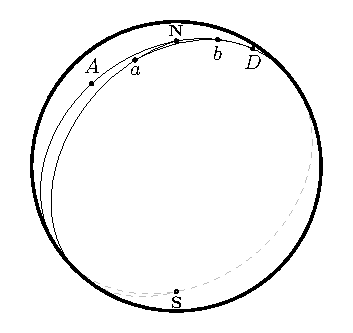
\includegraphics[width=.3\textwidth]{fig/chpt01/sphere.pdf}
    \caption{共轭点}
\end{wrapfigure}

如图,球面的南北极 $\mathbf N,\mathbf S$ 间存在无数等长测地线.从 $\mathbf S$ 出发到 $D$ 的测地线可以是 $\mathbf S A \mathbf N D$.但其长度甚至并非极小.


测地线, 其长度却并非极小, 因其非常邻近的曲线 $s b \cup \gamma$ 比它还短. 测地线 sand 的长度之所以不是极小, 关键在于线上有北极点 $n$, 它与南极点 $s$ “共轭” , 即存在从 $s$ 到 $n$ 的与测地线 $\gamma_1$ “无限邻近” 的测地线 $\gamma_2$ ( “共轭点对” 的准确定义见选读 7-6-3). 

可以证明, 测地线长度取极小值的充要条件是线上不存在共轭点对. 欧氏空间当然没有共轭点对, 因此两点之间直线(段)最短.


曲线 $s b \cup \gamma$ 在 $b$ 点不可微, 严格说应在 $b$ 点附近对它 “磨光”, 磨光后的曲线的长度与 $s b \cup \gamma$ 的长度 “要多接近有多接近”.



地线. 再讨论一般时空. 设 $C$ 是 $p, q$ 间长度极大的类时线,则由定理 3-3-6 可知它是测地线. 然而反过来却未必,因为定理 3-3-6 只保证 $p, q$ 间的类时测地线长取极值, 不保证它是极大 (当然, 由于类光曲线长度为零, 它肯定也不是极小. ). 可以证明,任意时空中类时测地线长为极大的充要条件是线上不存在共轭点对. 


 对任意时空中有类时联系的两点: (1)两点间的最长线是类时测地线; (2)两点间的类时测地线未必是最长线(对闵氏时空一定是); (3)两点间没有最短类时线.


Cauchy 发展

\section{整体双曲时空}

渐近平直时空的共性变换

引力能量非定域性

Cauchy 动力学与奇点定理

\section{Penrose 过程}

\section{能量条件}
\section{奇点定理}


类光 Raychaudhuri 方程
\section{Witten 迅捷性}
陷俘面
\section{宇宙监督假设}
\section{高-Wald 定理}


   % 因果结构
    \chapter{实验理论}\label{chpt:experiment}

\section{等效原理}\label{sec:eq-prin}



引力理论的检验标准当然是科学的基础——实验,为此自然需要一个关于引力实验本身的理论,这样就可从实验结果依据实验理论来评判引力理论。Dicke 从 1960s 开始所从事的实验研究使人们对等效原理的理解逐渐深刻,并意识到应把等效原理摆在引力理论的约束这一地位上。

Galileo 性 $m_I=m_G$ 可准确地称为\textbf{弱}(weak)\textbf{等效原理},简称 WEP。Einstein 将力学实验推至一切物理实验的等效原理则称 \textbf{Einstein 等效原理},简称 EEP。亦有学者称之\textbf{强}(strong)\textbf{等效原理},简称 SEP。
不过,Will\cite{Will18} 选择区分 EEP 和 SEP。他将 EEP 表述为:

    1. \textit{WEP 成立};

    2.\textbf{局域 Lorentz 不变性}:\textit{任何局域非引力实验的结果与观者 4-速无关};
    
    3.\textbf{局域位置不变性}:\textit{任何局域非引力实验的结果与其时空点本身无关}。

\noindent 注意局域一词仍指空间点。之后又在 SEP 的表述中强调\textbf{自引力系统}\footnote{自引力系统(self-gravitating system)指各部分由引力聚集或能产生引力场的系统,大到恒星、行星,小到日常所见的物体皆于考虑之列。}与测试粒子一样遵守 WEP,且将局域 Lorentz 和位置不变性中的非引力实验换为任意实验。可见这种要求似乎更强,它不仅考虑系统所处的外引力场,还考虑系统内物体所激发的自引力场,即引力的主被动方面皆考虑。
它们对引力理论选择的具体影响如何?目前任何引力理论都满足 WEP,因为验证很早就已开始且精度较高,这件近乎铁打的事实使人很难寻找一个不符 WEP 的理论。可论证若 EEP 成立,则引力一定是时空几何效应,严格满足一个度规理论的基本性质:

1.\textit{时空上能定义度规};

2.\textit{自由的测试粒子的世界线满足该度规下的测地线方程};

3.\textit{局域惯性系中非引力物理定律满足狭义相对论}。

\noindent 前文已从 WEP 窥探到 2 的成立。又可证\textbf{Schiff 猜想}(conjecture):凡完备且自洽的满足 WEP 的理论皆必须满足 EEP。当然,引力的度规理论是很多的,除了广义相对论,还有 Brans-Dicke 理论。

 由于目前已知的度规理论除广义相对论均不满足 SEP,故有人提出:若 SEP 成立,广义相对论可能是唯一选择。关于这一命题的讨论目前还不够严格,故只能算猜想。
目前学术界对等效原理的分类未达成共识,Ohanian\cite{Ohanian} 就批评用自引力系统强行区分 WEP 和 EEP。对此无法说得更通俗了,只有在我们学会后续知识后才能有更深理解。

上述所有论证细节和具体实验均放入

WEP 目前最精确的检验是 21 世纪于太空中完成的,得到铝、铂间 $m_G/m_I$ 的差异小于 $10^{-14}$,且数据在地球上空各处基本一致;关于 EEP,对量子非引力实验的描述需用波函数,而波函数至少散布在一个区域内,这样强引力场的潮汐效应会显现在波函数中,但可选择对弱引力场中的小区域波函数进行实验,已有数据显示这种量子系统可满足;SEP 目前最精确的检验利用了地月测距(lunar-laser-ranging),测得两天体间 $m_G/m_I$ 的差异不大于 $5.5\times 10^{-13}$,引力结合能的贡献差异不大于 $1.3\times 10^{-3}$。


\section{几何}


\section{后 Newton 近似}

\section{引力波}

\section{宇宙学}   % 实验验证
    \chapter{引力波初步}\label{chpt:wave}
本章附录将简要回顾现代量子力学理论和形式的基本经验事实,以及最初的理论尝试。随后将给出其数学和计算结构,以及其所成功解决的物理问题。最后将描述其所致的概念自洽性问题——这至今尚未得以解决。

引力辐射   % 引力波
    \chapter{宇宙学初步}\label{chpt:cosmos}
空间均匀的宇宙学模型
\section{运动学}
\section{动力学}
\section{热力学}
\section{标准模型疑难}
\section{暗能量}
\section{暴涨理论}   % 宇宙学
    
    %\part{附录}
    \begin{appendices}
        \chapter{范畴论}\label{appx:cat}
首先,默认读者已熟悉主要的集合、映射与关系知识,包括差集、交并补运算律、卡氏积(Cartisian product)、指标集、可数性、等价类、划分、幂集、陪域、逆像、双射等概念。若对这些概念有所遗忘,可查阅任意分析学、代数学教材以复习。

请读者大致回顾至今学习的\textit{所有知识}。我们遇到过各种各样的事物,它们之间又存在着各种联系:从整数之间的大小比较,到集合之间的映射,再到线性空间之间的同构。1940 年代,MacLane 为研究代数拓扑、线性代数中自然同构的问题,试图抽象这一思想,将各个东西及其间的联系,放到一个整体的学说中研究。这些“东西”称为\textbf{对象}(object),它们之间的关系用箭头(arrow)表示,称为\textbf{态射}(morphism)。
指定一组对象构成的集合及其间所有态射之集,就给出了一个\textbf{范畴}(category)。
范畴论将我们熟知的知识进行进一步的抽象封装。
我们不关心一个集合里具体有什么,而是把每个集合看作一个对象;不关心究竟把某个元素映射至何处,而是把映射单纯地看成箭头,研究集合上任意映射之集。
如此,全体集合构成\textbf{集合范畴} $\cate{Set}$。
我们有了一种更为普适、简洁的视角去看待很多理论。

不仅如此,由于这些理论中的态射都具有相似性质(比如复合函数的结合性),这意味着这些理论实质上有非常紧密的联系待发掘。利用范畴论,就很容易找到不同理论之间的对应,比如欧氏几何和用代数表达图形的解析方法。甚至,可将某个理论的概念套进范畴的模版里,进一步发展原有的理论。
在范畴论里,\textit{关系就是一切}。许多情况下,一个数学对象完全由它与所有其他对象的关系决定。换言之,当且仅当两个对象以同样方式与范畴中的每个对象相关时,两个对象本质上是不可区分的。这是著名的\textbf{米田引理}(Yoneda lemma)的一个推论。这同我们的日常经验相符,你大可通过观察一个人的社交关系来确定其性格;若你发现两个社交媒体账号,其关注和动态高度一致,则有理由推断此二账号同属一人。于是,范畴论可以成为构建一个数学理论的蓝图,被称为\textit{数学的数学}。

剩下的关键在于对态射需设置何种要求。一般希望态射的复合具有结合性,且存在到自身的态射。为保证足够的抽象和普适性,这可以是全部的要求了:
\begin{definition}
    设两集合 $\mathrm{Ob},\mathrm{Mor}$,它们之间配上一对映射
     $\begin{tikzcd} \mathrm{Mor} \arrow[yshift=-0.5ex, r, "t"'] \arrow[yshift=0.5ex, r, "s"] & \mathrm{Ob} \end{tikzcd}$。
    将 $\mathrm{Ob}$ 的元素称作\textbf{对象},$\mathrm{Mor}$ 的元素称为\textbf{态射}。对某个态射 $f\in\mathrm{Mor}$,映射 $s,t$ 的像分别指明其\textbf{来源}(source)和\textbf{目标}(target),也即域和陪域。
    对 $X, Y \in \mathrm{Ob}$,记 $\hom(X, Y) := s^{-1}\{X\} \cap t^{-1}\{Y\}\subset\mathrm{Mor}$,称为 $\hom$-集,其元素称为从 $X$ 到 $Y$ 的态射。
    
    态射还满足如下要求。对任意对象 $X$ 都存在 $\mathrm{id}_X \in \hom(X, X)$,称为 $X$ 到自身的\textbf{恒等}(identity)\textbf{态射}。可证同个对象的任意两个恒等态射是相等的,故其实恒等态射是存在且唯一的。对任意 $X, Y, Z \in \mathrm{Ob}$,给定态射间的\textbf{复合}(composition)
        \begin{align*}
            \circ : \hom(Y, Z) \times \hom(X, Y) & \longrightarrow \hom(X, Z), \\
            (f, g) & \longmapsto f \circ g,
        \end{align*}
        不致混淆时常将 $f \circ g$ 简记为 $fg$,满足
        \begin{itemize}
            \item 结合律(associativity),即对任意 $h, g, f \in \mathrm{Mor}$,若复合 $f(gh)$ 和 $(fg)h$ 都有定义,则 $f (g h) = (f g) h$。
            故两边可以同写为 $f \circ g \circ h$ 或 $fgh$;
            \item 对任意 $f \in \hom(X,Y)$,有 $f \circ \mathrm{id}_X = f = \mathrm{id}_Y \circ f$。
        \end{itemize}
    $(\mathrm{Ob},\mathrm{Mor})$ 称为一个\textbf{范畴}。常记 $\mathcal C=(\mathrm{Ob}(\mathcal C),\mathrm{Mor}(\mathcal C))$。对象及其态射常记作 $X\xrightarrow{f} Y$ 的形式。
\end{definition}

著名的 \textbf{Russell 佯谬}考虑了所有集合构成的“集合” $\textbf{V}$,利用\textbf{自我指涉}的思想,构造其子“集合” $\{x \in \textbf{V} : x \notin x\}$ 可导出矛盾。现代集合论处理此问题的主流方法是限制概括原理
\[\left\{x : x \text{ 满足性质 } P\right\}\]
的应用范围,并在一阶逻辑与合适的公理系统下进行演绎。以上提到的“集合” $\textbf{V}$ 实非集合,而称作\textbf{类}(class)。凡集合都是类,但还存在非集合的类,称作\textbf{真类}。通过使用元语言并避开额外逻辑可以承认类的存在性,因为用 Russell 佯谬推出矛盾需要额外的逻辑。故原则上Ob, Mor可以是一般的类,比如 Ob$(\cate{Set})$ 是真类。

图表加箭头是讨论范畴的方便语言。用箭头表达态射,用箭头的头尾衔接表示复合映射。最常用的是\textbf{交换图}(commutative diagram),“交换”意指箭头的复合殊途同归,例如
    \[ \begin{tikzcd}
        X \arrow[rr, "f"] \arrow[rd, "h"'] & & Y \arrow[ld, "g"] \\
        & Z &
    \end{tikzcd} \qquad \begin{tikzcd}
        A \arrow[r, "u"] \arrow[d, "x"'] & B \arrow[d, "v"] \\
        C \arrow[r, "y"'] & D
    \end{tikzcd} \]
的交换性分别等价于 $g f = h$ 和 $v u = y x$。态射的名称若自明或不重要,则常从图中略去。

\begin{definition}
    对于态射 $X \xrightarrow{f} Y$,若存在 $Y \xrightarrow{g} X$ 使得 $f g = \mathrm{id}_Y,g f = \mathrm{id}_X$,则称 $f$ 是(对象)\textbf{同构}(isomorphism),而 $g$ 称为 $f$ 的\textbf{逆},从恒等态射的性质易见逆若存在则唯一。从 $X$ 到 $Y$ 的同构集记作 $\mathrm{Isom}(X, Y)$。

    记 $\operatorname{End} X := \hom(X, X),\operatorname{Aut} X := \mathrm{Isom}(X, X)$,分别称作 $X$ 的\textbf{自同态集}和\textbf{自同构集}。这些集合在二元运算 $\circ$ 下封闭,或用代数的语言来说:$\operatorname{Aut} X$ 是群,
    $\operatorname{End} X$ 是幺半群。若忘记其定义可见下节。
\end{definition}

一个范畴往往代表一套理论。研究范畴间的关系可进一步抽象出如下概念:
\begin{definition}
    设 $\mathcal{C}', \mathcal{C}$ 为范畴。映射 $F: \mathcal{C}' \to \mathcal{C}$ 称为\textbf{函子}(functor),包括:
    \begin{enumerate}
        \item 对象间的映射 $F: \mathrm{Ob}(\mathcal C')\to\mathrm{Ob}(\mathcal C)$.
        \item 态射间的映射 $F: \mathrm{Mor}(\mathcal C')\to \mathrm{Mor}(\mathcal C)$, 使得
            \begin{itemize}
                \item $F$ 与来源和目标映射相交换 (即 $sF=Fs$, $tF=Ft$),或等价地,对每个 $X, Y \in \mathrm{Ob}(\mathcal{C}')$ 皆有映射 $F: \hom_{\mathcal{C}'}(X, Y) \to \hom_{\mathcal{C}}(F(X), F(Y))$。换言之,$f\in \hom_{\mathcal{C}'}(X, Y)\Rightarrow F(f)\in \hom_{\mathcal{C}}(F(X), F(Y))$;
                \item $F(g\circ^{\prime} f) = F(g) \circ F(f)$,$F(\mathrm{id}_X) = \mathrm{id}_{F(X)}$。
            \end{itemize}
    \end{enumerate}
    对于 $F: \mathcal{C}_1 \to \mathcal{C}_2,G: \mathcal{C}_2 \to \mathcal{C}_3$,\textbf{复合函子} $G \circ F: \mathcal{C}_1 \to \mathcal{C}_3$ 的定义显然是取相应复合映射:$\mathrm{Ob}(\mathcal{C}_1) \xrightarrow{F} \mathrm{Ob}(\mathcal{C}_2) \xrightarrow{G} \mathrm{Ob}(\mathcal{C}_3)$ 和 $\mathrm{Mor}(\mathcal{C}_1) \xrightarrow{F} \mathrm{Mor}(\mathcal{C}_2) \xrightarrow{G} \mathrm{Mor}(\mathcal{C}_3)$。
\end{definition}

上述函子又称为\textbf{协变函子}。交换图表述为
\[\begin{tikzcd}
    X \arrow[r, "f"] \arrow[d, "F"'] & Y \arrow[r, "g"] \arrow[d, "F"'] & Z \arrow[d, "F"]\\
    F(X) \arrow[r, "F(f)"] & F(Y) \arrow[r, "F(g)"] & F(Z).
\end{tikzcd}\]
相应地,\textbf{逆变函子}就是将关于复合映射的性质改为 $F(f):F(Y)\to F(X),F(gf) = F(f) \circ F(g)$,故交换图为
\[\begin{tikzcd}
    X \arrow[r, "f"] \arrow[d, "F"'] & Y \arrow[r, "g"] \arrow[d, "F"'] & Z \arrow[d, "F"]\\
    F(X) & \arrow[l, "F(f)"'] F(Y) & \arrow[l, "F(g)"'] F(Z).
\end{tikzcd}\]

可以考虑反转某个范畴的所有箭头,而反转后范畴论的公理依然成立,范畴论中的这种对称性也称作对偶原理:
\begin{definition}
    范畴 $\mathcal{C}$ 的\textbf{反范畴}(opposite category)或\textbf{对偶范畴} $\mathcal{C}^\mathrm{op}$ 定义如下:
    \begin{itemize}
        \item $\mathrm{Ob}(\mathcal{C}^{\mathrm{op}}) = \mathrm{Ob}(\mathcal{C})$;
        \item 对任意对象 $X, Y$,$\hom_{\mathcal{C}^{\mathrm{op}}}(X, Y) := \hom_{\mathcal{C}}(Y, X)$;
        \item 态射 $f \in \hom_{\mathcal{C}^{\mathrm{op}}}(Y, Z), g \in \hom_{\mathcal{C}^{\mathrm{op}}}(X, Y)$ 在 $\mathcal{C}^{\mathrm{op}}$ 中的复合 $f \circ^\mathrm{op} g$ 定义为 $\mathcal{C}$ 中的反向复合 $g \circ f$;
        \item 恒等态射定义同 $\mathcal{C}$.
    \end{itemize}
\end{definition}
容易验证 $\mathcal{C}^\text{op}$ 满足范畴定义,且 $(\mathcal{C}^\text{op})^{\text{op}} = \mathcal{C}$。在处理许多范畴论性质时,善用对偶原理能省事不少。比如,逆变函子其实即形如 $F: (\mathcal{C}')^\text{op} \to \mathcal{C}$ 的(协变)函子。

研究函子间的态射可进一步抽象:
\begin{definition}
    函子 $F, G: \mathcal{C}' \to \mathcal{C}$ 之间的\textbf{自然变换}(natural transformation) $\theta$ 是一族态射 $\{\theta_X\}$,其中 $\theta_X \in \hom_{\mathcal{C}}(F(X), G(X))$ 且 $X \in \mathrm{Ob}(\mathcal{C}')$,使得下图对所有 $\mathcal{C}'$ 中的态射 $f: X \to Y$ 交换:
    \begin{equation}\begin{tikzcd}
        F(X) \arrow[r, "\theta_X"] \ar[d, "F(f)"'] & G(X) \arrow[d, "G(f)"] \\
        F(Y) \arrow[r, "\theta_Y"] & G(Y) .
    \end{tikzcd}\end{equation}
    上述自然变换写作 $\theta: F \Rightarrow G$,或图解为
    \[ \begin{tikzcd}
        \mathcal{C}' \arrow[bend left=50, r, "F", ""' name=U] \arrow[bend right=50, r, "G"', "" name=D] & \arrow[Rightarrow, to path=(U) -- (D) \tikztonodes, "\theta"] \mathcal{C}.
    \end{tikzcd} \]
    上述带有双箭头的图表有时也被称为 \textbf{2-胞腔}(2-cell)。
\end{definition}

实用中经常会省略严格的范畴论框架,只说态射 $\theta_X: F(X) \to G(X)$ 对于变元 $X$ 是\textbf{自然的}或\textbf{典范的}(canonical),或称满足\textbf{函子性}。

任意函子 $F$ 到自身有恒等的 $\mathrm{id}_F : F \Rightarrow F$。对于 $\theta: F_1 \Rightarrow F_2$,若 $\psi: F_2 \Rightarrow F_1$ 满足 $\psi \circ \theta = \mathrm{id}_{F_1}$,$\theta \circ \psi = \mathrm{id}_{F_2}$,则称 $\psi$ 是 $\theta$ 的逆。可逆的自然变换称为\textbf{函子同构}。由定义直接看出 $\theta$ 的逆若存在则是唯一的,记作 $\theta^{-1}$,它无非是在范畴中\textit{逐点}取逆:$(\theta^{-1})_X := (\theta_X)^{-1}: F_2 X \to F_1 X$。同理可见 $\theta$ 可逆当且仅当任意 $\theta_X$ 可逆(同构)。函子同构 $\theta: F_1 \Rightarrow F_2$ 的等价说法是称 $\theta_X: F_1 X \to F_2 X$ 对变元 $X$ 是\textbf{自然同构}或\textbf{典范同构}。更抽象的概念纳入到了\textbf{高维范畴论}的领域。
   % 范畴学
        \chapter{点集拓扑}\label{appx:topo}

18 世纪,Euler 等人发现简单多面体的顶点数 $v$、楞数 $e$、面数 $f$ 总是满足 $v-e+f=2$。
具体地,简单多面体可连续变化成球面。用投影来模拟这个过程:多面体内应存在一种位置,在此处放一盏灯,各顶点和棱都投影在一个外部球面上,这些棱的投影曲线彼此不穿过。比如凸多面体和某些凹多面体,但像厚球壳那样带腔、像甜甜圈那样带洞的多面体是不行的。
这种变化还可形象地视作捏橡皮膜(rubber-sheet),拓扑学因而又称为\textbf{橡皮几何}。的确,自然界存在直觉上形状相似的几何体,为抽象出共性,可试着“揉”它但不撕裂或粘帖,观察是否能得到另一几何体,如从正方体到球体。这种连续变化间的等价性称作\textbf{同胚}(homeomorphism)。$v-e+f$就是一个多面体在同胚下保持不变的量,即\textbf{拓扑不变量}。
进而我们能将各几何体分门别类,注意力集中于诸如“是否有内外”“是否有洞”“绳上打了几个结”这类问题上的,从而架空距离、面积这些传统几何概念。一个典型例子是,对于理想电路,无论接线长度、方向如何,只要节点不变,电路网络就是等价的。

\begin{figure}[ht]
    \centering
    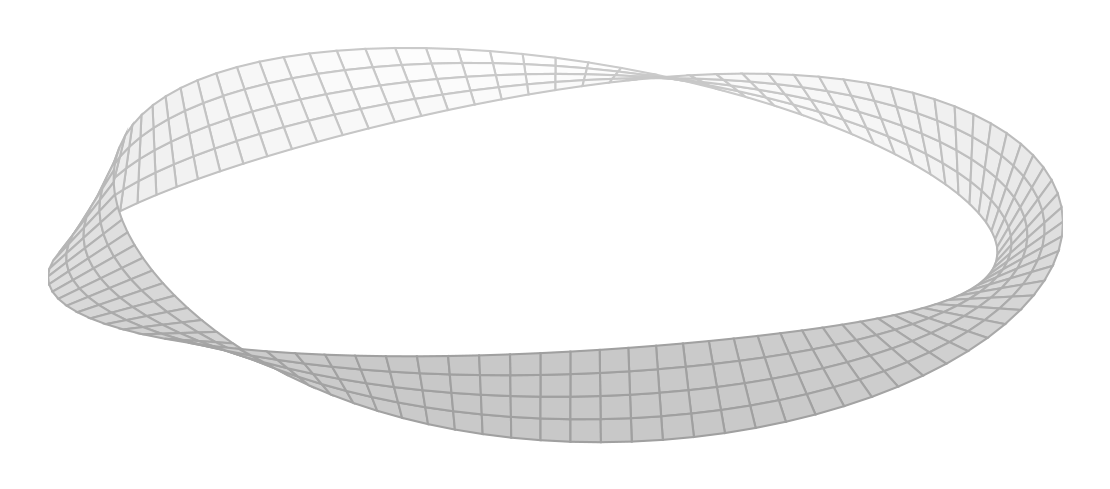
\includegraphics[width=.8\textwidth]{fig/appx/Mobius.png}
    \caption{M\"obius 环}\label{mobius}
\end{figure}

必须指出,用橡皮形变来比喻同胚仍有其局限性。一条纸带不经扭曲,可直接首尾连接得到手环,它具有两个面。扭转半周再相连将得到 M\"obius 环,它只有一个面。扭转一周再相连则又恢复为两个面。这个新环与最初的手环同胚,但却不能通过“揉捏”的方式恢复。如果我们注意到曲面的维度比背景空间的低,而只想关注曲面的内禀性质,则两种手环将视为同⼀空间在 $\R^3$ 内的不同表⽰。所谓的“揉捏”法,实质是 $\R^3$ 的⾃同胚。单看⼆者固然可建⽴同胚,但这种同胚⽆法扩张到整个 $\R^3$ 上。换言之,不存在从 $\R^3$ 的自同胚把两种手环映射在一起,这就解释了问题。这警示我们应更为抽象地看待拓扑。

正如上述例子一样,19 世纪末,人们欲抛掉坐标系而寻求一般集合的拓扑理论。为此要回到同胚的特征:拓扑变化的连续性借助于实数上的 $\epsilon$-$\delta$ 语言,故我们应给出一般集合的连续表述。这一时期可以称为拓扑的分析化,孕育出了\textbf{点集拓扑}。可以说此即最普适的拓扑学。构造这一理论花了很长时间,但我们可简述其关键:极限定义用到了实数集上的小于(序结构)和减法(度量结构),这相当于规定哪类子集是某点邻域、开集和闭集。
因此,拓扑学所研究的对象可以看作脱胎于距离的一种更广义的空间。将这些关键概念抽离出来后,我们就能在拓扑框架下重新得到分析学的定义、命题。现代主流拓扑学正是从这些分析概念出发,一步步走向具象的橡皮几何。
更为深刻的话题将涉及\textbf{代数拓扑}。这一专题将在关于\textbf{上同调}(cohomology)的部分中得以处理,在讨论拓扑分类、积分理论时 de Rham 上同调比较好用。

\section{拓扑空间}

回忆一下,集合 $X$ 的幂集可表示为 $2^X$。$2^X$ 的子集称为\textbf{子集族}(collection of subsets),故全体子集族又构成 $2^{2^X}$。欲对 $X$ 中每个点挑选⼀族⼦集作为其邻域(neighbourhood),即邻域族,就是给定映射 $\mathscr N:X\to 2^{2^X}$ 且 $\mathscr N(x)\ne \mt$。
直观上,邻域只需含有 $x$ 即可,但由于大小任意,可无限接近于 $x$,故有“邻”称。
若 $A\in \mathscr N(x)$,则 $x$ 为 $A$ 的内点(interior point),而 $A$ 中全体内点之集 $A^\circ$ 就是其内部(interior)。

希望从分析学中抽取邻域的若干性质,但不能太多,因为要普适到能包括不同于通常定义的情形。新表述不能依赖距离概念。关键在于,注意属于、包含等集合术语,已能描绘距离所表达的含义:$x$ 在其任意邻域内;$x$ 的任意两邻域之交也是 $x$ 的邻域;$x$ 的任意邻域的内部也是其邻域;包含 $x$ 某邻域的集合也是其邻域。
有了邻域,其它概念都好办了:在某全集 $X$ 下,开集(open set)是满足 $A=A^\circ$ 的集合,闭集(closed set)是其补集为开的集合。因此 $\mt,X$ 是既开又闭的。根据 $\epsilon$-$\delta$ 定义,$f:X\to Y$ 在 $x\in X$ 连续,即 $\forall\epsilon>0$ 都 $\exists\delta>0$,使得 $x$ 的 $\delta$ 邻域的像含于 $f(x)$ 的 $\epsilon$ 邻域。

往往直接考察 $f$ 整体的连续性,但邻域毕竟是就某 $x\in X$ 而言的,可预料从开集出发语言将更优雅。非空开集总是某点的某邻域,而邻域的内部必开,故 $f$ 的连续性表述不必出现邻域概念。有两点考虑:$f$ 不一定是满射,但空集可作为 $Y\backslash\Im f$ 的逆像;$f$ 不一定是单射,满足 $f(z)=f(x)$ 的 $z$ 可以很多,但 $f$ 的连续性要求处处连续,因此 $f(x)$ 任意邻域的逆像一定是所有 $z$ 的某邻域之并。综上,$f$ 连续即 $Y$ 中任意开集之逆是 $X$ 的开集。

由于包含邻域之集也是邻域,因此任意开集之并为开;而两邻域之交为邻域,经由归纳法,只能保证有限个开集之交为开;$\mt,X$ 是开的,$x\in X$ 的邻域则是能包含某个含有 $x$ 的开集的集合。这几条性质显然能导出邻域体系,故为等价表述。

\begin{definition}
$\mathscr{T}\subset 2^X$ 称为 $X$ 的一个\textbf{拓扑}(topology),若:
\begin{itemize}
    \item $\mt,X \in \mathscr{T}$;
    \item $\forall \sigma\subset \mathscr{T}$,$\bigcup_{U\in\sigma} U\in \mathscr{T}$;
    \item $U,V\in\mathscr{T}\To U\cap V\in\mathscr{T}$。或等价地对有限集 $\{A_{i}\} \subset \mathscr{T}$,$\bigcap_{i} A_{i} \in \mathscr{T}$。
\end{itemize}
$\mathscr{T}$ 的元素称为 $X$ 在 $\mathscr{T}$ 下的\textbf{开子集},简称\textbf{开集}。
$(X,\mathscr T)$ 称为 $X$ 关于拓扑 $\mathscr T$ 的\textbf{拓扑空间}。拓扑空间的元素称为\textbf{点}(point)。
\end{definition}

\begin{definition}
    对$x\in X,U\subset X$,若 $\exists O\in\mathscr{T}$ 使 $x\in O\subset U$,则 $U$ 是 $x$ 的一个\textbf{邻域}。$x$ 的全体邻域构成 $\mathscr N(x)$。邻域为开则称\textbf{开邻域},构成 $\mathscr N(x)\cap\mathscr T$。
\end{definition}

\begin{definition}
    $A\subset X$ 称为\textbf{闭集},若 $X\backslash A\in\mathscr{T}$。
\end{definition}

$\mathscr T$ 的名称若自明或不重要,则拓扑空间常略写为$X$。讨论开集时也常省略全集。De Morgan 律指出:并集之补等于补集之交,因此闭集也能给出拓扑的定义。容易得出等价表述为:$\mt,X$ 是闭的;有限闭集之并为闭;任意闭集之交为闭。

拓扑的选取有很多。若 $\mathscr T_1\subset\mathscr T_2$,则称 $\mathscr T_1$ \textbf{较粗}(coarser)或 $\mathscr T_2$ \textbf{较细}(finer)。直观上,较细拓扑容纳更多开集,能区分更多点。\textbf{凝聚}(indiscrete)\textbf{拓扑} $\mathscr T=\{\mt,X\}$ 最粗。\textbf{离散}(discrete)\textbf{拓扑} $\mathscr T= 2^X$ 最细。
分析学中,$\mt$ 和能表为开区间之并的集合都是 $\R$ 上开集,构成 $\R$ 的\textbf{通常}(usual)\textbf{拓扑} $\mathscr T_u$。视 $x,y\in\R$ 的距离为 $|x-y|$,则开区间实质是以 $\frac{x+y}{2}$ 为心的一维球。$(\R,\mathscr T_u)$ 称为\textbf{实直线}。通常拓扑当然比离散、凝聚拓扑更直观,后者一般用于构造反例。

\begin{definition}
    对 $(X,\mathscr T_X),(Y,\mathscr T_Y)$,$f: X \to Y$ \textbf{连续},若 $\forall A\in\mathscr T_Y$,$f^{-1}[A]\in \mathscr T_X$。
\end{definition}

\begin{definition}
    双向连续的双射称作\textbf{同胚}。显然,若空间同胚,则拓扑同势,即开集结构等同。
\end{definition}

\begin{remark}
    同胚的逆也必须连续。考虑复平面上的单位圆周 $C:|z|=1$。按 $f(x)=\e^{\i x}$ 定义 $f:[0,2\pi)\to C$。它是连续双射,但逆不连续。而直观上圆周与区间不能同胚。
\end{remark}

\begin{definition}
置 $(X,\mathscr T)$ 和 $A\subset X$。
\textbf{内部}为开集 $A^\circ:=\bigcup_{O\in\mathscr T\cap 2^A} O$,也即含于 $A$ 的最大开集。
\textbf{闭包}(closure)为闭集 $\bar{A}:=\bigcap_{X\backslash B\in\mathscr T,A\subset B} B$,也即包含 $A$ 的最小闭集。
$\partial A=\bar{A}\backslash A^\circ$ 称为 $A$ 的\textbf{边界}(boundary)。
\end{definition}

\begin{remark}
    显然 $A^\circ\subset A\subset \bar A$。$A^\circ\cup\partial A=\bar A$,$A^\circ\cap\partial A=\mt$。
    
    $\partial A=\mt\iff A^\circ=A=\bar A\iff A$ 既开又闭。
\end{remark}

\begin{theorem}
    $(X\backslash A)^\circ=X\backslash \bar A$。
\end{theorem}
\begin{proof}
    根据定义,$A^\circ:=\bigcup_{X\backslash F\in\mathscr T,X\backslash F\subset A} X\backslash F=X\backslash\bigcap_{X\backslash F\in\mathscr T,X\backslash A\subset F} F=X\backslash\overline{X\backslash A}$。
    替换即可。
\end{proof}

\begin{theorem}
    $A$ 为开集 $\eqto A=A^\circ\eqto\forall x\in A,A\in\mathscr N(x)\eqto\forall x\in A,\exists U\in\mathscr N(x)$ 使 $U\subset A$。
\end{theorem}

\begin{proof}
    $A=A^\circ\in\mathscr T$;反之 $A\in\mathscr T,A\subset A\To A\subset A^\circ\iff A=A^\circ$。

    $A=A^\circ\iff\forall x\in A,\exists O\in\mathscr T$ 使 $x\in O\subset A\iff\forall x\in A, A\in\mathscr N(x)$。
    
    $\forall x\in A$ 下,$\exists U\in\mathscr N(x)$ 使 $U\subset A\To \exists O\in\mathscr T$ 使 $ x\in O\subset U\subset A \To A\in\mathscr N(x)$;反之 $\exists A\in\mathscr N(x)$ 使 $A\subset A$。
\end{proof}

\begin{theorem}
    $A$ 为闭集 $\iff A=\bar A$
\end{theorem}
\begin{proof}
    $A$ 为闭集 $\iff X\backslash A=(X\backslash A)^\circ=X\backslash\bar A\iff A=\bar A$。
\end{proof}

\begin{theorem}
    $x\in\bar A\iff\forall U\in\mathscr N(x),U\cap A\ne\mt$。
\end{theorem}
\begin{proof}
    给定 $x\in\bar A$,假设 $\exists U \in\mathscr N(x),U \cap A=\mt$。则 $\exists O\in\mathscr T$ 使 $x\in O\subset U\To A\subset X \backslash U\subset X \backslash O$,$X \backslash O$ 为闭集 $\To \bar{A} \subset X \backslash O\iff O \cap \bar{A}=\mt$,矛盾;
    给定 $\forall U\in\mathscr N(x),U\cap A\ne\mt$,假设 $x\in X \backslash \bar{A}$。则 $X \backslash \bar{A}\in\mathscr T\To \exists X \backslash \bar{A}\in\mathscr N(x),(X \backslash \bar{A}) \cap A=A \backslash \bar{A}=\mt$,矛盾。
\end{proof}

\begin{definition}
置 $A\subset X$。\textbf{导集}(derived set)为 $A':=\{x \in X:x\in\overline{A\backslash\{x\}}\}$,其元素称为\textbf{聚点}(accumulation point)或\textbf{极限点}。
$\bar{A}=X$ 时称 $A$ 在 $X$ 中\textbf{稠密}(dense)。
\end{definition}
\begin{remark}
    $x\in A'\eqto \forall U\in\mathscr N(x),(U\cap A)\backslash\{x\}=U\cap (A\backslash\{x\})\ne\mt$。$U$ 可等价换为任意含 $x$ 开集。
\end{remark}
\begin{eg}
    考虑实直线,$0,1/2,1$ 都是 $[0,1)$ 的聚点。
\end{eg}

\begin{theorem}
    $\bar A=A\cup A'$。  
\end{theorem}

\begin{proof}
    任给 $x\in A'$。$\forall U\in\mathscr N(x),(U\cap A)\backslash\{x\}\ne\mt\Rightarrow \forall U\in\mathscr N(x),U\cap A\ne\mt\eqto x\in\bar A$。说明 $A'\subset \bar A$,此 $A\cup A'\subset\bar A$;
    任给 $x\in\bar A\backslash A'$。$x\in\bar A,x\notin A'\eqto \exists U\in\mathscr N(x),(U\cap A)\backslash\{x\}=\mt$ 且 $U\cap A\ne\mt\Rightarrow U\cap A=\{x\}\Rightarrow x\in A$。说明 $\bar A\backslash A'\subset A\iff \bar A\subset A\cup A'$。
\end{proof}

\begin{theorem}
    $A$ 为闭 $\iff A'\subset A$。
\end{theorem}
\begin{proof}
    $A$ 为闭 $\iff A=\bar A\iff A=A\cup A'\iff A'\subset A$。
\end{proof}

\begin{definition}
    $S:\N\to X,n\mapsto x_n$ 的值域 $\Im S=\left\{x_n\right\}$ 称为\textbf{序列}或\textbf{点列}。
    若 $\exists x \in X$,$\forall U\in\mathscr N(x),\exists N\in\N$,使 $n>N\To x_n\in U$,则称 $\{x_n\}$ 有\textbf{极限}或\textbf{收敛}于 $x$。
\end{definition}

\begin{remark}
    点列聚点的任意邻域都含点列的无限个点。极限是聚点,但聚点不一定是极限。
\end{remark}

\begin{definition}
    在 $(X,\mathscr T)$ 下,可定义 $A \subset X$ 的\textbf{相对}(relative)\textbf{拓扑}或\textbf{诱导}(induced)\textbf{拓扑} $\mathscr T_r=\{O \cap A: O\in\mathscr T\}$。赋予诱导拓扑的子集称为原集的\textbf{拓扑子空间}(topological subspace)。
\end{definition}

\begin{eg}
    对于实直线和 $A=[0,2]$,在 $\mathscr T_u$ 的诱导下 $B=(1,2]$ 是 $A$ 中的开集。
\end{eg}

\begin{definition}
    给定 $(X,\mathscr T_X),(Y,\mathscr T_Y)$ 和 $Z=X \times Y$。
    定义
    \[\mathscr T_Z=\{O\subset Z:A\in\mathscr T_X,B\in\mathscr T_Y,\text{$O$ 可表为形如 $A\times B$ 的集合之并}\},\]
    $(Z,\mathscr T_Z)$ 称为 $X,Y$ 的\textbf{乘积拓扑空间}(product topological space)。
\end{definition}

这与 $\R$ 的通常拓扑类似,都是通过囊括空集和“任意并”操作来生成拓扑。这一方法可总结如下。取 $\mathscr{B} \subset 2^X$,首先它能覆盖整个 $X$:$\bigcup_{U\in\mathscr{B}}U=X$,其次保持“有限交”性质:对任意有限集 $\{U_i\}\subset\mathscr{B}$,$\exists\mathscr{F}\subset \mathscr{B}$ 使 $\bigcup_{U\in\mathscr{F}}U=\bigcap_{i} U_i$,就称$\mathscr{B}$ 为\textbf{拓扑基}。
$\mathscr{T}=\left\{\bigcup_{U\in\mathscr{F}}U:\mathscr{F}\subset\mathscr{B}\right\}$ 称为 $\mathscr{B}$ 生成的拓扑。\textbf{拓扑子基}的元素所有可能的有限交构成拓扑基。

许多空间往往都难以直接想象或处理,我们可考虑将它分解为简单直观的部分,再重组回去,就能描述复杂的拓扑空间。
设 $\tilde X=\{[x]:x\in X\}$ 是 $(X,\mathscr T)$ 在某个等价关系下的分割或商集(quotient set)。对其规定如下拓扑:映射 $\pi: X \to \tilde X,x\mapsto [x]$ 称为\textbf{自然映射}或\textbf{典范投影},取 $\tilde{\mathscr T}=\{U \subset Y:\pi^{-1}(U)\in\mathscr T\}$,称为\textbf{商拓扑},$(\tilde X,\tilde{\mathscr T})$ 称为\textbf{商空间}。可见,$\pi$ 就好比用来粘合拓扑空间的胶水。
可以证明,设 $\tilde{\mathscr T}^{\prime}$ 为 $\tilde X$ 上另一个拓扑,且使 $\pi$ 连续,则 $\tilde{\mathscr T}^{\prime} \subset \tilde{\mathscr T}$。

\section{度量空间}

我们看到,$\R$ 的距离便可生成一个拓扑基。距离概念的推广自然是在任意集合中,给定满足三角不等式、正定性的对称实函数。开区间也可相应地推广。

\begin{definition}
    \textbf{度量空间}(metric space)是集合 $X$ 和\textbf{距离函数}(或\textbf{度量})$d: X \times X \to [0,\infty)$ 的卡氏积,$\forall x,y,z\in X$ 满足:
    \begin{itemize}
        \item $d(x,y)=d(y,x)$;
        \item $d(x,y) = 0\eqto x=y$;
        \item $d(x,z) \leqslant d(x,y)+d(y,z)$。(三角不等式)
    \end{itemize}
    $B(x,r)=\{y \in X: d(x, y)<r\}$ 称为以 $x \in X$ 为中心、$r$ 为半径的\textbf{开球}(open ball)。
    总可用局部性质构造拓扑:全体开球 $\{B(x,\epsilon):x\in X,\epsilon >0\}$ 就是一个拓扑基,其生成拓扑 $\mathscr T_d$ 就是 $(X,d)$ 的\textbf{度量诱导拓扑},构成 $(X,d,\mathscr T_d)$。称 $(X,\mathscr T_d)$ 是\textbf{可度量的}。
\end{definition}

\begin{remark}
    原则上可以有负定的距离,就像度规一样,但这种距离一般不用于诱导拓扑。
    实际上,具有应用意义的拓扑空间大多都是度量空间。
\end{remark}

\begin{eg}
    \textbf{离散度量}满足 $d_{0}(x,y)=1$ 若 $x \ne y$。这是一个描述离散拓扑的办法。
\end{eg}

\begin{definition}
    置度量空间 $X$。度量 $d_{1},d_{2}$ 是\textbf{等价度量},若 $\exists a,b>0$,使对 $\forall x,y \in X$,有 $a d_{1}(x, y) \leqslant d_{2}(x, y) \leqslant b d_{1}(x, y)$。
\end{definition}

\begin{remark}
    显然等价度量诱导出相同拓扑。
\end{remark}

\begin{eg}
    置 $x=\left(x^1,\cdots,x^{n}\right),y=\left(y^{1},\cdots,y^{n}\right)\in\R^{n}$。$p$-度量为
\[
d_{p}(x, y):=\left(\sum_{k=1}^{n}\left|x^{k}-y^{k}\right|^{p}\right)^{1 / p},\quad p \geqslant 1.
\]
常取$p=2$,称为\textbf{欧氏度量}。
$\R$ 的开球即开区间。$\R^2$ 的开球称为\textbf{开圆盘}。极限为
\[
d_{\infty}(x,y):=\lim_{p\to\infty}d_{p}(x, y)=\max _{1 \leqslant k \leqslant n}\left\{\left|x^{k}-y^{k}\right|\right\}.
\]
任意 $p$-度量等价,诱导出通常拓扑 $\mathscr T_u$。当然,亦可视作 $\R$ 通常拓扑的乘积拓扑。
\end{eg}

我们已悉知 $\epsilon$-$\delta$ 语言可视为连续性在通常拓扑的特例。现在再用度量空间重新叙述。
置 $(X,d_X,\mathscr T_X),(Y,d_Y,\mathscr T_Y)$ 和映射 $f:X\to Y$。$f$ 在 $x \in X$ 处对度量诱导拓扑连续,当且仅当 $\forall\epsilon>0,\exists\delta>0$ 使 $B(x,\delta) \subset f^{-1} [B(f(x),\epsilon)]$。
即 $f^{-1} [B(f(x),\epsilon)]$ 是 $x$ 点邻域。
换言之,$d_X(x,x^{\prime})<\delta\Rightarrow d_Y(f(x),f(x^{\prime}))<\epsilon$。
若 $f$ 在任意点连续,即 $\forall x \in X,\epsilon > 0$,$f^{-1} [B(f(x),\epsilon)]\in\mathscr T_X$,结合“任意并”性质和逆像的保并性,可知 $\forall U\in\mathscr T_Y$,$f^{-1}[U]\in\mathscr T_X$,即 $f$ 连续。

对于度量空间,点列 $\left\{x_n\right\}$ 收敛于 $x$ 等价于 $\lim_{n\to\infty}d(x, x_n)=0$。
点列称为基本列或 Cauchy 列,即$\forall\epsilon>0,\exists N\in\N$使 $k,l>N\Rightarrow d(x_{k},x_{l})<\epsilon$。
度量空间称为\textbf{完备的}(complete),若其中任意 Cauchy 列都收敛于其中的点。实直线上闭区间完备,但开区间不完备:只需注意 $\{1/n\}_{n=2}^\infty$ 在 $(0,1)$ 上无极限。$\R^{n}$ 当然完备。
一致连续性即 $\forall \epsilon>0,\exists\delta>0$ 
使 $\forall x_{1},x_{2} \in X$,$d(x_{1},x_{2})<\delta\Rightarrow d(f(x_{1}),f(x_{2}))<\epsilon$。
注意一致连续要更强:对整个空间要求一致的 $\delta$。

\begin{definition}
    度量空间 $X$ 的子集称为\textbf{有界的},若存在开球包含它。否则称\textbf{无界的}。
\end{definition}

\begin{remark}
    完备性、有界性都不是拓扑不变性。例如,$(0,1)$ 与实直线同胚,但前者不完备、有界,后者完备、无界。
\end{remark}

置度量空间 $X$。$f: X \to X$ 称为(严格)\textbf{压缩映射}(contraction),若 $\exists c\in(0,1)$,使 $\forall x,y \in X$ 且 $x\ne y$,有 $d(f(x),f(y)) \leqslant c d(x,y)$。
仿照分析学可类似证明 \textbf{Banach 不动点定理}:若度量空间 $X$ 完备,$f$ 为一个压缩映射,则 $f(x)=x$ 的解存在且唯一。这是非线性泛函分析的一个有用工具。

\section{紧致性与连通性}

分析学给出了若干等价的实数定理,其中一条是著名的\textbf{Heine-Borel 有限覆盖定理}:若闭区间能被某个开集族覆盖,则可从其中找到有限多元素,构成依旧能覆盖的子族。
19 世纪中叶,Dirichlet 在试图严格化函数连续性时,率先用有限覆盖技术,证明了闭区间上的连续实函数一致连续。
不过他的结果半个世纪后才发表,期间 Heine, Weierstrass 等人各自独立地用类似技术也证明了该结论。Borel 利用这些技术证明了上述的有限覆盖定理。后来 Lebesgue 等人才把它推广到了一般情形。

有限覆盖定理叙述的内容实际上也是一个集合有界闭的充要条件。“有界闭”就是实数闭区间的推广描述。有界性是与距离密切相关的,但有限覆盖性只涉及开集。可见关于有界闭集的分析学命题,很多都能延伸到点集拓扑。

\begin{definition}
    置 $(X,\mathscr T)$。
    $\mathscr C\subset\mathscr T$ 称为 $A\subset X$ 的\textbf{开覆盖}(open cover),若 $A\subset\bigcup_{O\in\mathscr C}O$。
    $\mathscr S\subset\mathscr C$ 是 $\mathscr C$ 的\textbf{子覆盖}(subcover),若它也是开覆盖。若 $\mathscr S$ 是有限集,则称 $\mathscr C$ 存在\textbf{有限子覆盖}。
    $A$ 称为\textbf{紧致的}(compact)或\textbf{紧的},若其任意开覆盖都存在有限子覆盖。
\end{definition}

\begin{eg}
    拓扑基当然是 $X$ 的一个开覆盖。
\end{eg}

\begin{eg}
    实直线上,单点集 $\{x\}\subset X$ 必紧。$\R$、开区间、半开区间非紧。
\end{eg}
\begin{proof}
    对 $\{x\}$ 任取开覆盖 $\mathscr C$,则 $\exists O\in\mathscr C$ 使 $x\in O$,$\{O\}$ 即有限子覆盖。
    不妨以 $(0,1]$ 为例,存在开覆盖 $\{(1/n,2):n\in\N\}$ 不具有限子覆盖;其余情形同理。
\end{proof}

\begin{eg}[Heine-Borel]
    实直线上,闭区间等价于紧集。
\end{eg}

\begin{definition}
    \textbf{仿紧}
\end{definition}


可数公理

\begin{definition}
    \textbf{第二可数}
\end{definition}
给出有用的拓扑结构,使点足够稠密但又不至于太怪异,称为几何背景。

分离公理

\begin{definition}
    拓扑空间 $X$ 称为 $T_2$ 或 \textbf{Hausdorff 的},若对任意不同的两点 $x,y \in X$,存在 $x$ 的开邻域 $A$ 与 $y$ 的开邻域 $B$,使得 $A \cap B=\mt$。
\end{definition}

以拓扑空间为对象、连续映射为态射可构建\textbf{拓扑空间范畴} $\cate{Top}$。

\begin{theorem}
    显然度量空间是 $T_2$ 的。
\end{theorem}

这看起来更像我们所期待的。但是,某些略微非 $T_2$ 的空间会很有用。
\begin{eg}
    在扭量(twistor)理论中。一个“口袋”(pocket)提供了这样的一个例子。考虑实平面的子集 $X$,由实轴上的区间 $[-1,1]$ 和直线 $y=1$ 上的区间 $[0,1]$ 构成,并且等同如下的点:$(x,0) \approx(x,1),0<x \leqslant 1$ 。这样,点 $(0,0)$ 与 $(0,1)$ 就没有不相交的开邻域。严格说来,我们需要下文中商拓扑的概念。
\end{eg}

\begin{eg}
    一个更为地道的非 $T_2$ 空间:考虑正整数组成的空间 $\N_+$,开集取成 $\mt,\N_+$ 以及集合 $\{1,2,3,\cdots,n\}$。这个空间既非 $T_2$ 亦非紧致的(见后面关于紧致的定义)。
\end{eg}

\begin{definition}
    一个拓扑空间 $X$ 称为\textbf{连通的},如果它不能写成两个互不相交 的非空开集的并。有用的两条等价说法是: 任何一个从 $X$ 到赋予离散拓扑的两点集合 $\{0,1\}$ 的连续映射都不是满射;连通拓扑空间只有两个既开又闭的子集。

    给定一拓扑空间 $X$,定义一等价关系如下: $x \sim y$ 当且仅当 $x$ 和 $y$ 属于 $X$ 的 同一个连通子空间。则每个等价类称为 $X$ 的一个\textbf{连通分支}
\end{definition}

\begin{definition}
    设区间 $I\subset\R$ 和拓扑空间 $X$,连续映射 $C:I\to X$ 称为 $X$ 上的一条(有向)\textbf{曲线}(curve)。
    $\sigma\in I$ 称为曲线的\textbf{参数},$\Im C$ 称为\textbf{路径}(path),不混淆时亦可称曲线。
\end{definition}

\begin{definition}
    $C':I'\to $ 称为\textbf{重参数化}。严格单调
\end{definition}

\begin{definition}
    拓扑空间 $X$ 称为\textbf{路径连通的}(path-connected)或\textbf{弧连通的}(arcwise connected),如果 $X$ 中的任意两点都可被一条完全在 $X$ 中的路径连接。
\end{definition}

路径连通的拓扑空间一定是连通的。反之不一定,存在“擦边”的反例。流形的路径连通与连通等价,稍后叙述之。$\R^{n}$ 中的连通开子空间是路径连通的。

列紧性

$\R^{n}$ 中的任何有界序列有一个收敛子列

开球就是连通的

一般总能将非连通集视为有限个连通分支之并,不妨只考虑其中一个连通分支。连通集合称为\textbf{单连通的},就是说,其中任意形似橡皮圈的闭合曲线(称\textbf{简单闭线})所围成的任意曲面都含于此集合中。

单连通区域总同胚开球。

连通区域的表面正是\textbf{闭曲面}。
比如,闭曲面总能将 $\R^n$ 分为有界部分(即所包围区域)和无界部分,因此可区分空间的内外。
一般偏好将法矢取定为朝外,称为\textbf{外指}(outward-pointing)\textbf{法矢},简称\textbf{外法矢}。
单连通的表面就称\textbf{简单闭曲面},简单闭线可视作特殊情形。
物理学总是关注这种良好对象,比如求分段光滑的简单闭曲面的场通量,而实际上分析学的 Gauss 定理的确适用之。
   % 点集拓扑
        \chapter{线性代数拾遗}\label{appx:LA}

\section{线性空间}

带有满足结合律的二元运算的非空集称\textbf{半群}(semigroup)。存在单位元的半群称\textbf{幺半群}(monoid)。元素皆可逆的幺半群正是群。
\textbf{同态}(homomorphisms)是保持群结构的映射 $f \in \hom(G_1, G_2 ) \Leftrightarrow f (g_1 h_1 )=f (g_1 ) f (h_1 )$。
单位元和逆元是唯一的,因为假设 $\bar 1',\bar 1$ 是单位元,则 $\bar 1'=\bar 1'\bar 1=\bar 1$;假设 $z,\bar x$ 是 $x$ 的负元,则 $z=z\bar 1=z(x\bar x)=(zx)\bar x=\bar 1\bar x=\bar x$。

\textbf{环}(ring)具有两种分别称为加法和乘法的运算,其中加法应构成交换群(Abel 群),乘法应满足结合律,并同加法一起满足分配律。加法单位元称为\textbf{零元},加法逆元称为\textbf{负元}。不混淆时零元记作 $0$,而 $x$ 的负元记作 $-x$。
若乘法满足交换律,则称\textbf{交换环}或 \textbf{Abel 环}。存在乘法单位元的环称\textbf{幺环}。非零元在乘法上可逆的环称\textbf{除环}。交换幺除环称为\textbf{域}(field),常记作空心字符,如 $\mathbb{K}$。称域对其加法、乘法是\textbf{封闭的}。由于零元不可逆,故通常要求域首先至少有零元和乘法单位元。
环 $R$ 的一个\textbf{双边理想}(2-sided ideal) $I$ 是 $R$ 的一个子环,且满足 
\[r \in R, a \in I \Rightarrow r a \in I, a r \in I.\]
可用显然的方式定义\textbf{左理想}和\textbf{右理想}。

群、环、域都只考虑某个集合的\textbf{内部运算}。我们当然也能考虑另一集合来构造所谓的\textbf{外部运算}。通常我们会在群上,加上一个由环给出的外部运算,这就是某环上的\textbf{模}(module)。
给定环 $R$,\textbf{左 $R$-模} $X$ 是一个交换群,且带有另一称为外部乘法的运算 $R \times X \rightarrow X$,满足对 $\forall \alpha,\beta \in R, x,y \in X$ 有如下分配律和结合律:
\[(\alpha+\beta) x=\alpha x+\beta x,\quad \alpha(x+y)=\alpha x+\alpha y,\quad (\alpha\beta)x=\alpha(\beta x).\]
若 $R$ 是幺环,则还要求其乘法单位元 $1$ 使 $1x=x$。\textbf{右 $R$-模}的定义是显然的。

\textbf{代数}(algebra)首先是幺环 $R$ 上的模 $X$,且要给定另一称为乘积的内部运算,使得 $X$ 自身是环,并对 $\forall \alpha \in R, x,y \in X$ 有 $\alpha(xy)=(\alpha x) y=x(\alpha y)$。可见代数上有五种运算:$R$ 的加法和乘法、$X$ 的加法和乘积、外部乘法。

进而回顾一下,域 $\mathbb F$ 上的\textbf{线性空间}其实就是 $\mathbb F$-模。由于 $\mathbb F$ 是域,选取左模或右模其实无关宏旨。一般取实数域 $\R$ 或复数域 $\C$,相应有实线性空间和复线性空间。显然 $\mathbb F$ 自身可以成为 $\mathbb F$-线性空间。线性空间的元素称为\textbf{向量}或\textbf{矢量}。其中内部运算称为(逐点)加法,外部运算称为数乘。物理上常称为\textbf{线性叠加原理},而将矢量画成笔直的箭头。可以看到,$V$ 在赋予某种乘法后是一个代数,可称\textbf{线性代数},比如内积空间或者张量积空间。当然,线性代数在现在更多指此概念所发展的一套学说。

设线性空间 $V$。某非空 $S\subset V$ 内元素的全体线性组合构成子空间 $\operatorname{span}B$,称为由 $B$ 张成的。若存在线性无关的非空子集 $B$ 使 $\operatorname{span}B=V$,则称 $B$ 是 $V$ 的一个\textbf{基}(basis)或一组\textbf{基矢}(basis vectors)。若 $B$ 是有限集,则称 $V$ 是\textbf{有限维的},可定义维数 $\dim V:=|B|$。易知任意基的元素个数一致,由此维数是良定义的。若 $B$ 是无限集,也即任意有限矢量组 $\{e_\mu\}_{\mu=1}^n$ 都不构成基,则称 $V$ 是\textbf{无限维的}。典型例子是 $[a, b] \subset \R$ 上连续复函数构成无限维复线性空间 $C[a, b]$,直观上是因为 $[a, b]$ 有无穷多自由度,从而总存在函数不能有限表出。
映射 $A:V\to V$ 称为 $V$ 上的\textbf{算子}、\textbf{算符}(operator)或\textbf{变换}。
有限维里有很多结论不能简单推广至无限维,否定这些结论带来了更多“反直觉”的性质。相对论的物理量主要属于有限维。

\begin{definition}
    \textbf{泛函}严格指无限维 $V$ 上的函数。
\end{definition}

\begin{remark}
    曾用拉氏理论理解泛函,而 Fréchet 空间的确是无限维线性空间。
\end{remark}

易知 $x\in V$ 可由任意基 $\{e_\mu\}$ 唯一地线性表示,称系数组 $\{k^\mu\}$ 为 $x$ 由 $\{e_\mu\}$ 表出的\textbf{分量},有限维时写作 $(k^1,\cdots,k^n)^\mathrm{T}$。欲谈及同一矢量在不同基间的分量变换,先要给定基变换。
设 $\{e_\mu\},\{e'_\mu\}$ 是线性空间 $V$ 上两组不同的基,某矢量 $v\in V$ 在两组基下的分量分别是 $\{v^\mu\},\{v'^\mu\}$。设基矢 $e_\mu^{\prime}$ 在 $\{e_\mu\}$ 下的展开为
\eq{
e'_\mu=A^\nu{ }_\mu e_\nu,
}
其中 $A$ 也叫过渡矩阵。两个基皆线性无关,故过渡矩阵可逆。于是由 $v'^\mu e'_\mu=v^\nu e_\nu$ 得 $v'^\mu A^\nu{ }_\mu e_\nu=v^\nu e_\nu$,由基的线性无关性知 $v'^\mu A^\nu{ }_\mu =v^\nu$,故
\eq{
    v'^\mu=(A^{-1})^\mu{}_\nu v^\nu.
}
因此基变换和分量变换是互逆的。

\section{对偶空间}

以 $\mathbb F$-线性空间为对象、线性映射为态射,构建\textbf{线性空间范畴} $\cate{Vect}(\mathbb F)$。

置 $f\in\hom(V,W)$。线性变换或线性算子即取 $W=V$ 的 $f\in\operatorname{End} V$。$W=\mathbb F$ 时称为线性函数。设 $V$ 的一个基 $\{e_\mu\}$,对 $V$ 中任意矢量 $k^\mu e_\mu$ 有 $f\left(k^\mu e_\mu\right)=k^\mu f(e_\mu)$。故其实只要知道 $\{e_\mu\}$ 在 $f$ 下的像组 $\{f(e_\mu)\}$,则 $V$ 中任意矢量在 $f$ 下的像就确定了,即线性映射完全由基的作用效果确定。显然 $A\in\hom(U,V),B\in\hom(V,W)$ 的复合也线性,即 $BA\in\hom(U,W)$。

假若 $f$ 还是双射,则 $f\in\mathrm{Isom}(V, W)$ 且 $f^{-1}\in\hom(W,V)$。换言之,$V,W$ 的线性双射为同构。若存在同构,则称 $V,W$ 互为\textbf{线性同构的},记作 $U\cong V$。有限维时易证等价于 $\dim U=\dim V$。易知 $f$ 是单射时,核为 $\ker f:=\{\alpha\in V:f(\alpha)=0\}=\{0\}$;$f$ 是满射时像为 $\Im f=W$。秩为 $\rank f:=\dim \Im f$,可证满足 $\dim \ker f + \dim \Im f = \dim V$。故若 $f$ 单射,则 $\Im f\cong V$。对线性变换而言,这说明单射等价于满射。换言之,满秩线性变换乃 $V$ 自同构。

对任意线性空间 $V,W$,只要对 $\hom(V,W)$ 定义如下加法、数乘、零元:$\forall f,g\in \hom(V,W),v\in V,\alpha\in\mathbb F$ 有
\[(f+g)(v):=f(v)+g(v),\quad (\alpha f)(v):=\alpha f(v),\quad 0(v):=0,\]
则 $\hom(V,W)$ 成为了线性空间。一般考虑线性函数。称 $V^*=\hom(V,\mathbb F)$ 为\textbf{对偶空间},任意线性函数 $\omega\in V^*$ 称为\textbf{对偶矢量}。
比如,行向量空间就是列向量空间的对偶空间。
考虑从原来的 $V$ 来产生 $V^*$ 的基。方法是,假设 $\{e_\mu\}$ 是 $V$ 的一个基,则定义 $V^*$ 中有一组元素 $\{e^\mu\}$ 满足
\eq{ e^\mu(e_\nu):=\delta^\mu_\nu,}
进而由线性性可导出它对 $V$ 任意元素的作用情况,即 $e^\mu(A)=A^\mu$。再证明 $\{e^\mu\}$ 确实是一个基:对任意 $\omega\in V^*$ 设
\eq{
    \omega_\mu:=\omega(e_\mu),
}
则必能展开成 $\omega=\omega_\mu e^\mu$,因为两边作用于任意 $V$ 中元素即可,如 $\omega(e_\nu)=\omega_\mu e^\mu(e_\nu)=\omega_\nu$;显然线性无关:$0=\omega_\mu e^\mu(e_\nu)=\omega_\nu$。这说明 $\dim V^*=\dim V$ 或者 $V\cong V^*$。按此关系给出的 $\{e^\mu\}$ 就称 $\{e_\mu\}$ 的\textbf{对偶基}。

$V,V^*$ 间的同构当然是不唯一的。注意到 $\{e_\mu\}$ 到其对偶基 $\{e^\mu\}$ 的线性映射就是同构,那这会随着 $\{e_\mu\}$ 的不同选取而产生不同的同构。
若要有充分理由挑选出特殊同构,需另加结构限制之。
比如度规就建立了 $V,V^*$ 的特殊同构。

对偶操作不必继续“套娃”。设 $V^{**}=\hom(V^*,\mathbb F)$,下面说明可给 $V,V^{**}$ 找到同构,它不依赖于基的人为选取。用基底展开后有 $\omega(A)=\omega_\mu A^\mu=A^\mu\omega_\mu$,说明如果认为映射可交换,矢量也可成为对偶矢量的线性函数,只需定义 $i_V:V\to V^{**}$ 使得 $i_V A$ 满足 $i_V A(\omega):=\omega(A)$,
有时 $i_V A$ 简记作 $A^{**}$。显然 $i_V\in\mathrm{Isom}(V,V^{**})$。定义 $f\in\hom(V,W)$ 的对偶 $f^*\in\hom(W^*, V^*)$ 使得 $\forall\lambda\in W^*,A\in V$ 有
\eq{
    (f^*(\lambda))(A)=\lambda(f(A)).
}
显然恒等变换 $\mathrm{id}_V\in \operatorname{Aut} V$ 的对偶为 $\mathrm{id}_V^*=\mathrm{id}_{V^*}$;复合映射满足 $(f\circ g)^*=g^*\circ f^*$。进而取逆映射进行复合可知,若 $f$ 是同构则 $f^*$ 也是。
可证对任意线性 $f$,此同构是自然的:
\[\begin{tikzcd}
    V \arrow[r, "i_V"] \ar[d, "f"'] & V^{**} \arrow[d, "f^{**}"] \\
    W \arrow[r, "i_W"] & W^{**} ,
\end{tikzcd}\]
故被称为\textbf{自然同构}。$f$ 取决于对基的作用效果,故换言之,自然同构不依赖于基。实践中经常把自然同构直接写成等号,即 $V=V^{* *}$。将二者做认同后,省略同构符号可写成 $\omega(A)=A(\omega)$,数学上常写成 $\langle\omega,A\rangle$,这说明对偶矢量与矢量之间有天生的(god-given)乘法。且可证,不存在 $i_V\in\mathrm{Isom}(V,V^*)$ 使下图对任意线性 $f$ 交换:
\[\begin{tikzcd}
    V \arrow[r, "i_V"] \ar[d, "f"'] & V^{*} \\
    W \arrow[r, "i_W"] & W^{*} \arrow[u, "f^{*}"'],
\end{tikzcd}\]
故只有 $V,V^{* *}$ 间才能有自然同构。读者只需取以 $\R$ 为线性空间的特例就可证明。真正有用的是 $V,V^*$,好似两面镜子相互反射。

对偶基关系为 $\langle e^\mu,e_\nu\rangle=\delta^\mu_\nu$,因而当然也可把 $e^\mu$ 视作基而 $e_\mu$ 是其对偶基。只是遵从惯例,矢量的基使用下标,其对偶基是对偶矢量的基,用上标。设 $v=v^\mu e_\mu,\omega=\omega_\mu e^\mu$,当然 $v(\omega)=\omega(v)=v^\mu\omega_\mu$,自然有
\eq{
\omega_\mu=\omega(e_\mu),\quad v^\mu=v(e^\mu).
}
最后来研究各种分量、基变换的关系。
\begin{theorem}
    若 $V$ 中有一基变换 $e_\mu^{\prime}=A^\nu{ }_\mu e_\nu$,则相应的对偶基变换为
\eq{
e^{\prime \mu}=(A^{-\mathrm{T}})_\nu{ }^\mu e^{\nu}=(A^{-1})^\mu{ }_\nu e^{\nu}.
}
这说明对偶矢量 $\omega=\omega_\mu e^\mu$ 的坐标变换为 $\omega_\mu'=A^\nu{}_\mu\omega_\nu$。
\end{theorem}

\begin{proof}
    只需等式两边作用于 $e_\alpha^{\prime}$:
    \begin{align*}({A}^{-\mathrm{T}})_\nu{}^\mu\langle e^{\nu}, e_\alpha^{\prime}\rangle & =(A^{-\mathrm{T}})_\nu{ }^\mu A^\beta{}_\alpha\langle e^{\nu}, e_\beta\rangle  =(A^\mathrm{T})_\alpha{ }^\beta (A^{-\mathrm{T}})_\nu{ }^\mu \delta_\beta^\nu\\ &=(A^\mathrm{T})_\alpha{ }^\nu (A^{-\mathrm{T}})_\nu{ }^\mu=\delta_\alpha^\mu=\langle e^{\prime \mu}, e_\alpha^{\prime}\rangle,\end{align*}
    遂见结果相同。
\end{proof}

% 协变逆变的交换图

这种变换形式称为逆变,新量$=$矩阵$\times$旧量。原基底满足 $e_\nu={(A^{-1})}^\mu{}_\nu e^\prime_\mu$,称为协变,旧量$=$矩阵$\times$新量。

设 $Q\in V^{**}$ 在 $\{e^i\}$ 的对偶下的分量为 $Q^i=Q(e^i)$,则又回到了 式。这意味着可将它等同地视作切矢。



的\textit{基是协变的,其对偶基是逆变的}。进而可见矢量分量变换是逆变形式,因此也称 $V$ 中的矢量为\textit{逆变矢量}。这两种形式的变换之所以称为协变和逆变,其实是与线性空间基的变换相对比而来的。与矢量基相同形式变换的称为协变,与矢量基相反形式变换的称为逆变。

\section{张量空间}

\begin{definition}
    设 $\mathbb F$-线性空间 $\{X_i\}_{i=1}^k,W$。若
    $T:X_1\times\cdots\times X_k\to W$
    对任何 $X_i$ 都线性,则称\textbf{多重线性映射}。常取如下情形:
    \eq{
        T:\underbrace{V^*\times\cdots\times V^*}_{k\in\N}\times\underbrace{V\times\cdots\times V}_{l\in\N}\to \mathbb F,
    }
    称为 $V$ 上的一个\textbf{多重线性函数}或\textbf{张量}。如上即 $(k,l)$-张量,构成张量空间
\eq{
    \hom(\underbrace{V^*\times\cdots\times V^*}_{k\in\N}\times\underbrace{V\times\cdots\times V}_{l\in\N},\mathbb F)=:V^k_l.
}
\end{definition}
\begin{remark}
    用分号区分上下槽,如 $T(\oo;\oo,\oo)\in V^1_2$ 可输入 $\omega,v_1,v_2$ 得 $T(\omega;v_1,v_2)\in\mathbb F$。$T$ 视为全部槽为空时的简写。
\end{remark}

\begin{figure}[ht]
    \centering
    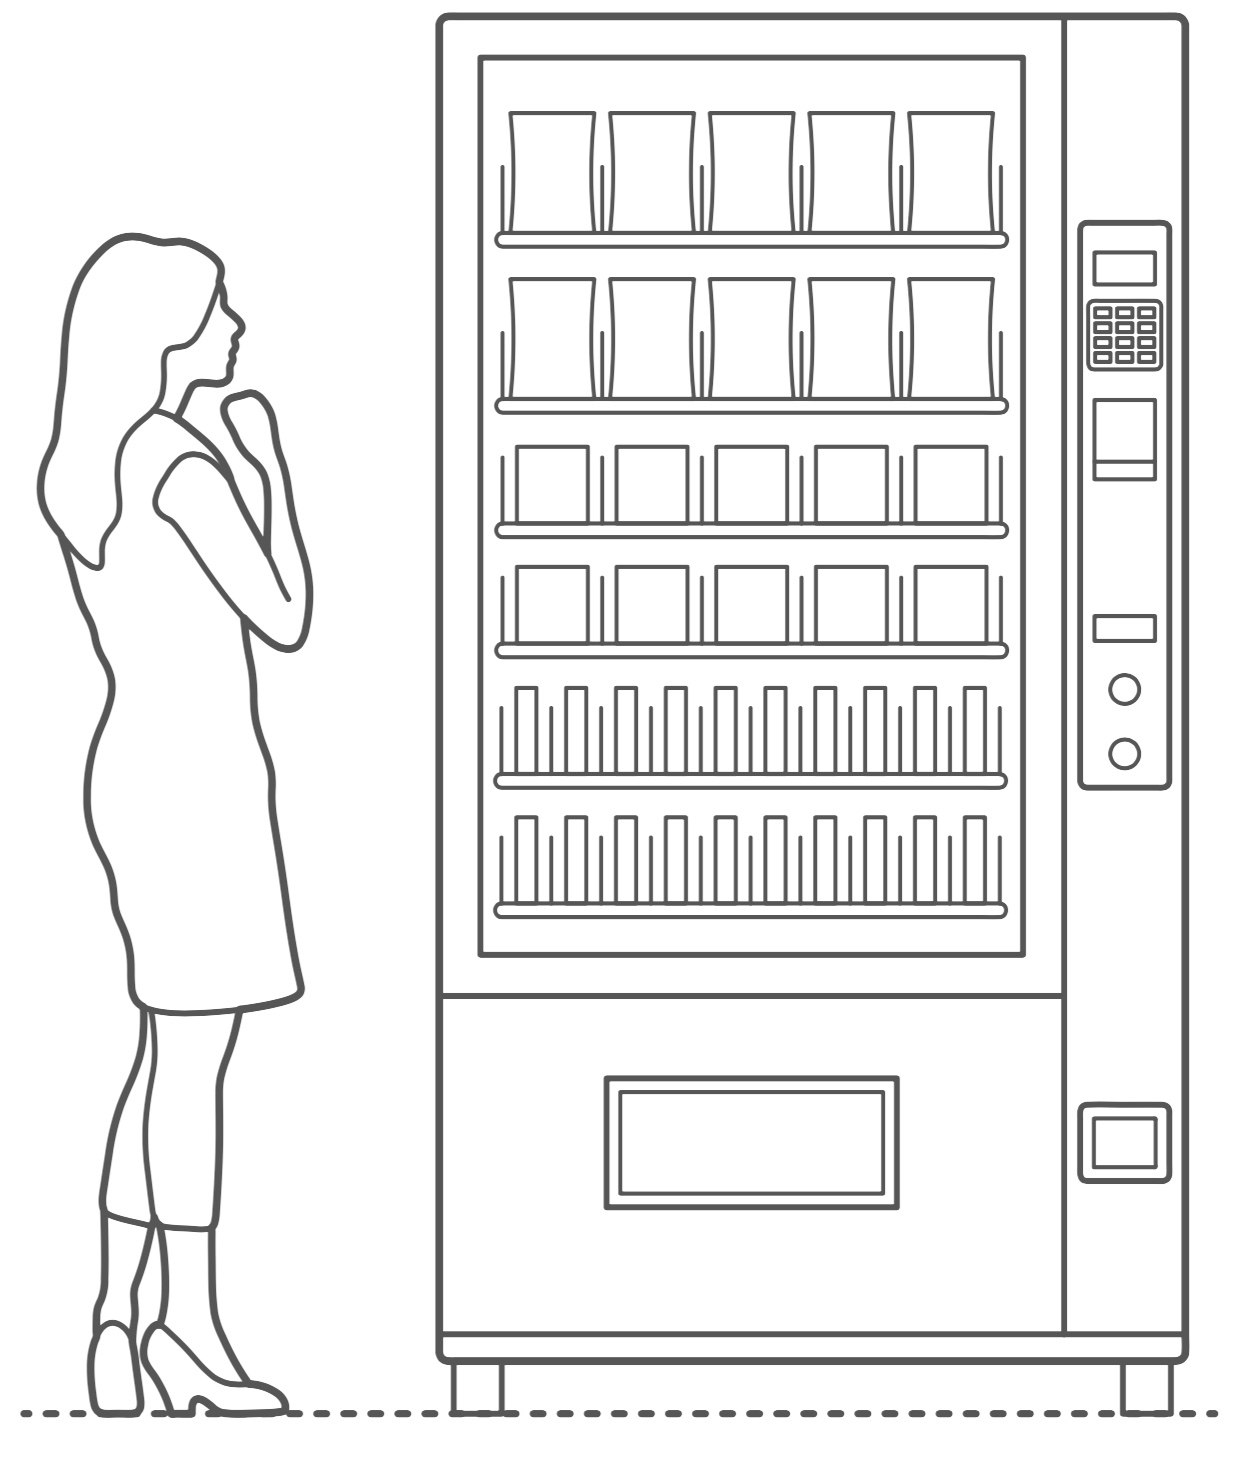
\includegraphics[width=0.4\textwidth]{fig/appx/vending.jpg}
    \caption{售货机}
    \label{fig:vending}
\end{figure}

张量与有限个矢量、对偶矢量线性地缩并出标量,因此可用多重线性函数表述。换言之,可直接称多重线性函数为张量,该定义多数情况与等价类 $[T^{\cdots}{}_{\cdots}]$ 表述等价。至少本节谈到张量均指多重线性函数。张量相比矢量、对偶矢量,无非是多出若干输入端口。
可类比从单元函数拓展到多元函数。如图 \ref{fig:vending},设想度规 $g$ 是一台具有两个槽(slat)的售货机,往槽中投入足够数量的一元纸币可获得一件商品,比如一听可乐。设某件商品需要两元纸币,则投入过程中,显示屏会不断改变数值以提示用户待支付的剩余金额,直至最终获得商品。这个过程类似于:
\[
    g(\oo,\oo)\To g(A,\oo)\in V^*\To g(A,B)\in\R.  
\]
关键在于,第一步输出的 $g(A,\oo)$ 将和之后输入的矢量 $B$ 线性地作用,最终输出实数,故相当于 $g(A,\oo)\in V^*$。类似地也有 $g(\oo,B)\in V^*$。
多重线性函数还可混合地输入矢量、对偶矢量,就好比售货机可以混合地投入硬币和纸币,只是对应的槽不同。
比如,$V$ 上的线性变换就是输入矢量且输出矢量,即 $X^\mu=T^\mu{}_\nu Y^\nu$,而矢量是对偶矢量的函数,因此线性变换又可看成矢量和对偶矢量的双线性函数,即 $(1,1)$-张量 $T^\mu{}_\nu$。比如 $\mathrm{id}_V$ 给出 $\delta^i_j A^j=A^i$,而 $\delta^i_j$ 单独看有上下槽。物理上有一例:应力张量涉及某个面上的压力,因此必定要先给定一个面法矢,这样就产生对应的一个作用力。

我们已熟知张量的线性组合、张量积、缩并,下面用映射语言重审之。

\begin{definition}  
取显然的加法、数乘、零元定义可使 $V^k_l$ 成为线性空间。这些运算即同型张量的线性组合,如 $T+ S+S+0=T+2S$。
\end{definition}

\begin{definition}
    $(k,l),(k',l')$ 型张量 $T,T'$ 的\textbf{张量积} $T\otimes T'$ 是一个 $(k+k',l+l')$-张量,使得
\begin{align}
    &T\otimes T'(\omega^1,\cdots,\omega^k,\omega^{k+1},\cdots,\omega^{k+k'};v_1,\cdots,v_l,v_{l+1},\cdots,v_{l+l'})\nonumber\\
    :=\ &T(\omega^1,\cdots,\omega^k;v_1,\cdots,v_l)\,T'(\omega^{k+1},\cdots,\omega^{k+k'};v_{l+1},\cdots,v_{l+l'}).
\end{align}
\end{definition}
\begin{remark}
    张量积有结合律,但一般不满足交换律。
\end{remark}
由于 $V^k_l$ 是线性空间,而 $V$ 有限维且 $k,l\in\N$,可讨论其维数:
\begin{theorem}
    $\dim V^k_l=(\dim V)^{k+l}.$
\end{theorem}
\begin{proof}
    设 $\{e_\mu\}$。可预料张量总能展为
    \eq{
        T={T^{\mu_1\cdots\mu_k}}_{\sigma_1\cdots\sigma_l}e_{\mu_1}\otimes\cdots\otimes e_{\mu_k}\otimes e^{\sigma_1}\otimes\cdots\otimes e^{\sigma_l},
        }
其中分量为
\eq{{T^{\mu_1\cdots\mu_k}}_{\sigma_1\cdots\sigma_l}:=T(e^{\mu_1},\cdots,e^{\mu_k};e_{\sigma_1},\cdots,e_{\sigma_l}),}
因为基底作用于相应基失的结果为
    \[e_{\mu_1}\otimes\cdots\otimes e_{\mu_k}\otimes e^{\sigma_1}\otimes\cdots\otimes e^{\sigma_l}(e^{\mu'_1},\cdots,e^{\mu'_k};e_{\sigma'_1},\cdots,e_{\sigma'_l})=\delta^{\mu'_1}_{\mu_1}\cdots\delta^{\mu'_k}_{\mu_k}\delta^{\sigma_1}_{\sigma'_1}\cdots\delta^{\sigma_l}_{\sigma'_l}.\]
基底显然线性无关。进而 $V_l^k=\mathrm{span}\{e_{\mu_1}\otimes\cdots\otimes e_{\mu_k}\otimes e^{\sigma_1}\otimes\cdots\otimes e^{\sigma_l}\}$。故 $\dim V_l^k=\prod_{i=1}^k\dim V^*\prod_{j=1}^l\dim V=(\dim V)^{k+l}$。
\end{proof}

张量空间实际上被视为\textit{线性空间张量积}的结果,即定义
    \eq{V^k_l=:\underbrace{V^*\otimes\cdots\otimes V^*}_{k\in\N}\otimes\underbrace{V\otimes\cdots\otimes V}_{l\in\N}.}
一般地,可定义不同线性空间的张量积为多重线性映射的 hom-集。换言之,矢量张量积是双线性映射 $\otimes:X\times Y\to W$,使得对任意线性空间 $Z$ 和双线性映射 $f: X\times Y\to Z$,都 $\exists!g\in\hom(W,Z)$ 满足 $f=g\circ\otimes$,即下图交换:
    \[ \begin{tikzcd}[row sep=small]
        X \times Y \arrow[rd, "f"'] \arrow[r] & X\otimes Y \arrow[d, "\exists!"] \\
        & Z.
    \end{tikzcd} \]
这称为张量积的\textbf{泛性质}。换言之,矢量张量积将 $X,Y$ 卡氏积变为其(线性空间)张量积。根据模论的相关定理,可证明 $X\otimes Y$ 一定存在,且同构意义下唯一。线性空间张量积可还原回张量及其张量积,故也是许多数学教材采用的等价定义。

\begin{theorem}
    设基变换 $e_\mu^{\prime}=A^\nu{ }_\mu e_\nu$,张量分量的变换律显然为
    \eq{
    T'^{\mu_1\cdots\mu_k}{}_{\nu_1\cdots\nu_l}=T^{\rho_1\cdots\rho_k}{}_{\sigma_1\cdots\sigma_l} (A^{-1})^{\mu_1}{ }_{\rho_1} \cdots(A^{-1})^{\mu_k}{ }_{\rho_k} A^{\sigma_1}{}_{\nu_1}   \cdots A^{\sigma_l}{}_{\nu_l}.
}
\end{theorem}
\begin{eg}
    线性变换 $T$ 的分量变换为 $T'^\mu{}_\nu= (A^{-1})^\mu{}_\rho T^\rho{}_\sigma A^\sigma{}_\nu$,即分量矩阵相似。双线性函数的分量变换为 $f'_{\mu\nu}=(A^\mathrm{T})_\mu{}^\rho f_{\rho\sigma} A^\sigma{}_\nu$,即分量矩阵合同。
\end{eg}

\begin{definition}
    $(k,l)$-张量 $ T $ 的第 $i$ 上标 $(i \leqslant k)$ 与第 $j$ 下标 $(j \leqslant l)$ 的\textbf{缩并}为
\eq{\c_{j}^{i} T:=T \big(\cdots,\hl{red}{e^{h}},\cdots ; \cdots,\hl[b]{blue}{e_{h}},\cdots\big),}
\hn{-2}{-1}{red}{第 $i$ 上槽}
\hn[b]{-2}{1}{blue}{第 $j$ 下槽}
\vspace{-0.1\baselineskip}

\noindent 其中对 $h$ 使用求和约定。缩并结果为 $(k-1,l-1)$-张量,且显然与基选择无关。
\end{definition}

缩并其实是求迹的映射版本,因此数学家会混记为 $\tr$。如线性变换 $T$ 在任意基底下矩阵的迹 $\tr T$ 就是 $(1,1)$-张量缩并,是基不变的标量。但两种符号的逻辑稍许不同:$\tr$ 是写出缩并后张量类型,$\c$ 是指明所缩指标位置。假设 $T$ 是一个 $(1,3)$-张量,定义 $S=\c^1_{2}T$,分量写法是 $S_{ij}=C^{k}{}_{ikj}$,但数学上记作 $S=\tr^0_2 T$。并且 $\tr$ 的用法有时并不唯一,比如 $S_{ij}$ 求迹必须借助升指标得 $g^{ij}S_{ij}$,数学上写作 $\tr_{g}S$。
将分量语言改写为映射语言时,只需注意“先张量积再缩并”可产生各种类型的新张量。可从映射语言直接看出,其结果相当于张量对矢量、对偶矢量的作用。比如,置 $T \in V^k_l,v \in V$,则
\begin{align*}
    \c_{\cdots}^{k+1}(T \otimes v)&=T \otimes v(\cdots,e^{\mu} ; \cdots,e_{\mu},\cdots)=T(\cdots;\cdots,e_{\mu},\cdots)v(e^\mu)\\
    &=T(\cdots;\cdots,v(e^\mu)e_{\mu},\cdots)=T(\cdots;\cdots,v,\cdots);
\end{align*}
同理 $T$ 对 $\omega\in V^*$ 作用其实即 $\c_{l+1}^{\cdots}(T \otimes \omega)$。
换言之,作用就是先积后并,简称\textit{作用即缩并}。

\begin{definition}
    张量 $T$ 关于某两下槽\textbf{对称},若 $\forall v,w\in V$ 有
    \[
    T(\cdots,v,\cdots,w,\cdots)=T(\cdots,w,\cdots,v,\cdots).
    \]
    \textbf{反称}即
    \[
    T(\cdots,v,\cdots,w,\cdots)=-T(\cdots,w,\cdots,v,\cdots).
    \]
    上槽同理。称多个槽对称或反称,若其中任意两槽对称或反称。若对所有上/下槽,则为\textbf{全对称}、\textbf{全反称}。显然张量的对称性和其分量的对称性一致,且无关基,故可视为等价定义。

    $T\in V^0_k$ 的对称、反称部分为
\eq{
\S T:=\frac{1}{k!}\sum_{\sigma\in S_k} \sigma T, \quad\A T:=\frac{1}{k!}\sum_{\sigma\in S_k} \sgn\sigma\,\sigma T,
}
其中 $\sigma T(e_{\mu_1},\cdots,e_{\mu_k})=T(e_{\mu_{\sigma(1)}},\cdots,e_{\mu_{\sigma(k)}})=T_{\mu_{\sigma(1)}\cdots\mu_{\sigma(k)}}$ 是 $T$ 按某一 $\sigma$ 给定的一个分量。其它情形同理。
\end{definition}

\begin{theorem}
    易证 $T=\S T\iff T=\sigma T$;$\omega=\A\omega\iff\omega=\sgn\sigma\,\sigma\omega$。
\end{theorem}

\begin{theorem}
    置 $f\in V^0_k,g\in V^0_l$,则 $\A(\A f\otimes g)=\A(f\otimes\A g)=\A(f\otimes g)$。证明思想与第 \ref{sec:co-di} 节的方法一致。
\end{theorem}

严格来说,由于不同型张量暂不能相加,故还未得到张量代数。设线性空间族 $\{X_i\}$。将 $X_1\times\cdots\times X_s$ 构造为线性空间,只需给定 $(x_1,\cdots,x_s)\oplus(y_1,\cdots,y_s)=(x_1+y_1,\cdots,x_s+y_s)$ 和 $\lambda(x_1,\cdots,x_s)=(\lambda x_1,\cdots,\lambda x_s)$ 即可。此即线性空间的\textbf{直和}(direct sum)。线性空间改记为 $X_1\oplus\cdots\oplus X_s$,元素改记为 $x_1\oplus\cdots\oplus x_s$。直和可从 $s\in\N$ 推广至可数无穷,但要求 $\bigoplus_{i=1}^\infty x_i$ 中仅有限个 $x_i$ 非零。\textbf{张量代数}定义为
\eq{
    V=\bigoplus_{k,l=1}^\infty V^k_l.
}
它显然是无穷维线性空间。张量积构成其乘法运算,故容易看出其的确是代数。这种构造类似于量子场论中 Fock 空间的构造 $V\to\mathscr H$,其中 $\mathscr H$ 是之后要学的单粒子 Hilbert 空间。

\section{内积空间}

仿照售货机例子和前文的降指标概念,可定义:

\begin{definition}
    设双线性映射 $f:V\times V\to W$。固定 $\alpha\in V$,与 $f$ 配合把 $\beta\in V$ 映到 $f(\alpha,\beta)\in W$ 的线性映射,记\footnote{五线谱的降记号 “$\flat$” 读作“降”(flat)、升记号 “$\sharp$” 读作“升”(sharp)。} $f_\flat(\alpha)=f(\alpha,\oo)$。$f_\flat\in\hom(V,\hom(V,W))$ 称为\textbf{降映射}。
\end{definition}


专注于 $W=\mathbb F$,则 $f$ 为双线性函数、$f_\flat(\alpha)$ 为对偶矢量、$f_\flat\in\hom(V,V^*)$。
双线性函数的分量矩阵称为\textbf{度量矩阵}。不同基的度量矩阵是合同的,而合同变换保秩,故可直接定义 $\rank f$ 为任意度量矩阵的秩。

\begin{theorem}
    $\rank f=\rank f_\flat$.
\end{theorem}

$f$ 满秩时称为非退化的。易证充要条件是分量矩阵可逆,或
\eq{\forall w \in V,\quad f(v,w)=0 \iff v=0.}
故非退化性等价于 $f_\flat\in\mathrm{Isom}(V,V^*)$。换言之,可规定好某个 $f$ 作为 $V$ 上的额外结构,建立 $V,V^*$ 间的特殊同构。

相对论主要用实线性空间。度规是 $\mathbb F=\R$ 的特例:

\begin{definition}
    $V$ 上一个对称、非退化的双线性实函数 g 称为 $V$ 上的一个\textbf{度规}。 $g_\flat:V\to V^*$ 称作\textbf{音乐同构}(musical isomorphism)或\textbf{典范同构}(canonical isomorphism)。度规逆 $g^{-1}:=g^{ij} e_i\otimes e_j$,或用 $\c^2_1(g^{-1}\otimes g)=\mathrm{id}_V$ 定义。
\end{definition}

\begin{definition}
    升降指标操作本质为音乐同构,故是相对于某度规而言的。比如 $(1,1)$-张量 $T$ 的降为
    $\c_1^1(g\otimes T)=T_\flat$。升指标用度规逆,即 $\c_1^1(g^{-1}\otimes T)=T^\sharp$。就矢量、对偶矢量而言,可将音乐同构称为度规对偶:$A\in V$ 的降为 $A_\flat:=g_\flat A$;$\omega\in V^*$ 的升是 $\omega^\sharp:=g^{-1}(\omega,\oo)$。
\end{definition}

\begin{remark}
    基和对偶基的对应通常不是度规对偶,即 $e^\mu\ne (e_\mu)_\flat, e_\nu\ne (e^\nu)^\sharp$。
\end{remark}

任意对称矩阵 $f_{ij}$ 总合同于某个对角阵,对应标准二次型,秩正是非零对角元的个数。且还可继续归一化,对应规范二次型。就实对称矩阵而言,对角元(特征值)符号可变:
\eq{(\tilde f_{ij})=\diag(\pm 1,\cdots,\pm 1,0,\cdots),}
但正、负或为零的\textit{个数}在合同变换下分别不变。正项个数称正惯性指数,负项个数称负惯性指数。简言之,合同变换保持正负惯性指数,此即代数学的 \textbf{Sylvester 惯性定理}。正负惯性指数之差就是号差,它进而是不变的。

度规的非退化性使其无零特征值,就可迎合物理上时空度规总能变换至 $\eta_{\mu\nu}$ 的要求。
记负惯性指数 $s$。$s=0$ 时称度规是\textbf{正定的}(positive definite)。$s=\dim V$ 时称\textbf{负定的}(negative definite)。其它皆称\textbf{不定的}(indefinite),时空度规就是不定的,推广到高维情形时,可依旧按东海岸习惯规定 $(-1,1,\cdots,1)$,西海岸取 $(1,-1,\cdots,-1)$。

使度规表为单位阵的基称为该度规下的\textbf{正交归一基},即满足 $g(e_i,e_j)=\pm\delta_{ij}$ 的$\{e_{\mu}\}$。当然,数学上内积的定义略有不同。首先对于 $\R$,数学上的内积通常正定:$\langle\alpha,\beta\rangle\geqslant0$,而正定内积必非退化。相对论允许不定度规,因此 $\alpha \in V$ 的模或\textbf{范数} $|\alpha|=\sqrt{|\langle\alpha, \alpha\rangle|}$ 需在根号中加绝对值。有时为与行列式区分写作 $\|\alpha\|$。最常用的写法是 $\alpha^2=\langle\alpha, \alpha\rangle$,允许模方为负。但都有 \textbf{Cauchy-Schwartz 不等式} $|\langle\alpha, \beta\rangle| \leqslant|\alpha \| \beta|$。$n$ 维线性空间在给定正定内积后,就成了 $n$ 维实内积空间,其不仅同构于 $\R^n$,且可在正交归一基,按勾股定理定义夹角、长度等概念,故有时也被称为\textit{欧氏(线性)空间}。其次对于 $\C$,数学通常发展了量子力学的态矢概念:
\begin{definition}
    复线性空间 $V$ 称为\textbf{复内积空间},简称内积空间,若给定内积运算 $(\oo, \oo): V \times V \rightarrow \C$,对任意 $f, g, h \in V$ 和任意 $c,d \in \C$ 满足:
    
    (第二槽线性性)$(f, cg+dh)=c(f, g)+d(f, h)$;
    
    (交换律)$(f, g)=\overline{(g, f)}$,其中 $\overline{(g, f)}$ 代表复数 $(g, f)$ 的共轭复数;
    
    (非退化)$(f, f) \geqslant 0$, 且 $(f, f)=0 \Leftrightarrow f=0$。
    \end{definition}
    \begin{remark}
        数域为 $\R$ 时退为正定内积。只含零元的线性空间也可构成内积空间,但下面只讨论维数大于零的情况。
    \end{remark}
    \begin{theorem}
    非退化条件配以线性性和交换律可得到 $(f+g, h)=(f, h)+(g, h)$ 及 $(c f, g)=\bar{c}(f, g)$。称内积对第一槽有\textbf{共轭线性}。
    \end{theorem}
    \begin{theorem}
    对非退化条件中取 $g=f$ 可有:$\forall g\in V,(f,g)=0\To f=0$。
    \end{theorem}
    \begin{eg}
        对 $C[a, b]$ 定义如下内积就构成内积空间:
    \eq{\label{b11}
    (f, g):=\int_a^b \overline{f(x)} g(x) \d {x}, \quad \forall f, g \in C[a, b].
    }
\end{eg}

对于有限维,从任意基 $\{\beta_i\}$ 出发,通过 \textbf{Gram-Schmidt 正交化}:
\eq{
\alpha_1=\beta_1,\quad \alpha_r=\beta_r-\sum_{k=1}^{r-1}\frac{(\alpha_k,\beta_r)}{(\alpha_k,\alpha_k)}\alpha_k,\quad \xi_i=\frac{\alpha_i}{|\alpha_i|},
}
总能找到内积空间中的正交归一基 $\{\xi_i\}$,其几何意义是正交投影和作差。这一正交化过程同样能用于寻找度规的正交归一基。

\begin{definition}
    置内积空间 $V$。对 $f,g\in V$ 的定义通常距离 $d(f, g):=\sqrt{(f-g, f-g)}$,便得到\textbf{度量线性空间}。该度量诱导拓扑之后,又成了\textbf{拓扑线性空间}。
\end{definition}

$\C$ 也能作为通常度量空间。以拓扑线性空间为对象、连续线性映射为态射,可构建\textbf{拓扑线性空间范畴} $\cate{TopVect}(\mathbb C)$。

\begin{definition}
    内积空间上全体连续线性函数之集称为其\textbf{共轭空间}或\textbf{对偶空间}。
\end{definition}
\begin{remark}
    有限维内积空间 $V$ 上的线性函数必连续,故 $\hom(V,\mathbb F)$ 等价于此处定义的对偶空间。
\end{remark}




\section{外代数}

本节主要考虑 $\mathbb F=\R$ 及有限维。

\begin{definition}
    $l$ 阶反称协变张量称为 \textbf{$l$ 次形式},简称 \textbf{$l$-形式}(form)。$V$ 上全体 $l$-形式之集记作 $\Lambda_l(V)$。
\end{definition}
\begin{remark}
    全反称即 $\omega=\A\omega=\sgn\sigma\,\sigma\omega$。沿用相应运算,$\Lambda_l(V)$ 显然是 $V^0_l$ 的线性子空间。
\end{remark}

标量、对偶矢量分别可称 0-形式、1-形式,可以预料 $\Lambda_l(V)$ 有自己的一套体系。张量通过张量积形成张量代数。形式也可通过某个封闭乘法形成所谓的\textbf{外代数}或 \textbf{Grassmann 代数}。但张量积对形式是不封闭的,如 $\omega_{[\mu\nu]}\zeta_{[\alpha\beta]}$ 并非 4-形式。我们需要一种全反称化操作,将张量积变为能保持形式性的乘法。并且,我们欲讨论 $\Lambda_l(V)$ 作为线性空间的维数,在构造基时也必须用保持形式性的乘法。

设 $n:=\dim V$。取对偶基 $\{e^\mu\}$,$l$-形式 $\omega$ 可表为 $\omega_{\mu_1\cdots\mu_l} e^{\mu_1}\otimes\cdots\otimes e^{\mu_l}$。由于反称性,$\omega$ 的独立分量仅在 $(\mu_1\cdots\mu_l)$ 为 $1,\cdots,n$ 的组合时。
欲讨论基和维数,必须考虑如何只用独立分量表示 $\omega$。且最好每一独立分量只用一次。新乘法记作 $\wedge$,则一般地希望
\eq{
\omega=\sum_{\mu_1<\cdots<\mu_l}\omega_{\mu_1\cdots\mu_l} e^{\mu_1}\wedge\cdots\wedge e^{\mu_l}=\frac{1}{l!}\omega_{\mu_1\cdots\mu_l} e^{\mu_1}\wedge\cdots\wedge e^{\mu_l},
}
求和下的排序相当于只对指标组合求和;而由反称性,$\wedge$ 对 $e^\mu$ 而言必须有反交换律,故可将求和换成除序因子。由 $\omega_{\mu_1\cdots\mu_l}=\omega_{[\mu_1\cdots\mu_l]}$ 或 $\omega=\A\omega$ 得
\[
    \frac{1}{l!}\omega_{\mu_1\cdots\mu_l} e^{\mu_1}\wedge\cdots\wedge e^{\mu_l}=\omega_{\mu_1\cdots\mu_l} \A(e^{\mu_1}\otimes\cdots\otimes e^{\mu_l}),
\]
说明希望
\[e^{\mu_{1}}\wedge\cdots\wedge e^{\mu_{l}}:=l!\A(e^{\mu_1}\otimes\cdots\otimes e^{\mu_l})=\sum_{\sigma\in S_l}\sgn\sigma\, e^{\mu_{\sigma(1)}}\otimes\cdots\otimes e^{\mu_{\sigma(l)}}.\]
另一方面,我们希望新乘法有结合性,这样任意两形式乘法就可以提出系数,而把它们的基凑在一起:
\[(e^{\mu_{1}}\wedge\cdots\wedge e^{\mu_{k}})\wedge( e^{\mu_{k+1}}\wedge\cdots\wedge e^{\mu_{k+l}}):= e^{\mu_{1}}\wedge\cdots\wedge e^{\mu_{k+l}}.\]
式右为
\[
(k+l)!\A( e^{\mu_{1}}\otimes\cdots\otimes e^{\mu_{k+l}})=(k+l)!\A\big(( e^{\mu_{1}}\otimes\cdots\otimes e^{\mu_{k}})\otimes( e^{\mu_{k+1}}\otimes\cdots\otimes e^{\mu_{k+l}})\big),
\]
因此考察两个形式之张量积与新乘法的联系:
\begin{align*}
    &(k+l)!\A\big(( e^{\mu_{1}}\wedge\cdots\wedge e^{\mu_{k}})\otimes( e^{\mu_{k+1}}\wedge\cdots\wedge e^{\mu_{k+l}})\big)\\
    =\,&(k+l)!\A\big(k!\A( e^{\mu_{1}}\otimes\cdots\otimes e^{\mu_{k}})\otimes l!\A( e^{\mu_{k+1}}\otimes\cdots\otimes e^{\mu_{k+l}})\big)\\
    =\,& k!l!(k+l)!\A\big(e^{\mu_{1}}\otimes\cdots\otimes e^{\mu_{k+l}}\big)=k!l!( e^{\mu_{1}}\wedge\cdots\wedge e^{\mu_{k}})\wedge( e^{\mu_{k+1}}\wedge\cdots\wedge e^{\mu_{k+l}}).
\end{align*}
综上我们给出
\begin{definition}
    任意 $k$-形式 $\omega$ 和 $l$-形式 $\mu$ 的\textbf{楔积}(wedge)为如下 $(k+l)$-形式:
    \eq{\omega\wedge\mu :=\frac{(k+l)!}{k!l!}\A(\omega\otimes\mu),\quad(\omega\wedge\mu)_{\nu_1\cdots\nu_k\lambda_1\cdots\lambda_l}=\frac{(k+l)!}{k!l!}\omega_{[\nu_1\cdots\nu_k}\mu_{\lambda_1\cdots\lambda_l]}.}
\end{definition}
\begin{remark}
    分量也可写成 $\omega_{\nu_1\cdots\nu_k}\wedge\mu_{\lambda_1\cdots\lambda_l}$。上文是阐述定义动机。显然从此出发可得上文全部结论,故为等价表述。
\end{remark}

\begin{eg}
    取 $n=3,l=2$,则
\begin{align*}
    \omega&=\omega_{12}e^1\otimes e^2+\omega_{21}e^2\otimes e^1+\omega_{13}e^1\otimes e^3+\omega_{31}e^3\otimes e^1+\omega_{23}e^2\otimes e^3+\omega_{32}e^3\otimes e^2\\
    &=\omega_{12}(e^1\otimes e^2-e^2\otimes e^1)+\omega_{13}(e^1\otimes e^3-e^3\otimes e^1)+\omega_{23}(e^2\otimes e^3-e^3\otimes e^2)\\
    &=\omega_{12}e^1\wedge e^2+\omega_{13}e^1\wedge e^3+\omega_{23}e^2\wedge e^3.
\end{align*}
\end{eg}

$\{e^\mu\}$的楔积即可作为 $\Lambda_l(V)$ 的基:由于已说明任意 $\omega$ 的表出,只需再说明线性无关性,而这是显然的。维度即独立分量数 $\dim\Lambda_l(V)=\binom{n}{l}=\frac{n!}{l!(n-l)!}$,其中 $l\leqslant n$。若 $l>n$,排完任意 $n$ 个指标后,根据抽屉原理,余下指标必存在重复,故所有分量为零,即此时 $\Lambda_l(V)=\{0\}$。通常默认 $0\leqslant l\leqslant n$。
\begin{theorem}拆到基底可知楔积的运算律有

    (结合律)$(\omega\wedge\mu)\wedge\nu=\omega\wedge(\mu\wedge\nu)$;

    (分配律)$\omega\wedge(\mu+\nu)=\omega\wedge\mu+\omega\wedge\nu$;

    (交换律)$\omega\wedge\mu=(-1)^{kl}\mu\wedge\omega$。
\end{theorem}

还可定义\textbf{全对称化}算子 $\mathrm{sym}:V^0_k\to V^0_k$ 和\textbf{全反称化}算子 $\alt:V^0_k\to V^0_k$:
\[\operatorname{sym} T:=k!\S T=\sum_{\sigma\in S_k} \sigma T,\quad \alt T:=k!\A T=\sum_{\sigma\in S_k} \sgn\sigma\,\sigma T,\]
对其它情形定义类似。置 $f\in V^0_k,g\in V^0_l$,则显然 $\alt(\alt f\otimes\alt g)=k!l!\alt(f\otimes g)$。楔积可表为 $\omega\wedge\mu=\frac{1}{k!l!}\alt(\omega\otimes\mu)$。基的楔积为 $e^{\mu_{1}}\wedge\cdots\wedge e^{\mu_{l}}=\alt( e^{\mu_{1}}\otimes\cdots\otimes e^{\mu_{l}})$。看上去系数仿佛改变。更有甚者直接将 $\omega\wedge\mu$ 定义为 $\Lambda(\omega\otimes\mu)$ 的形式,使得系数仿佛归一。故查阅不同书籍时请注意分辨。

\begin{theorem}
    $n$ 维线性空间上 $n$-形式 $\omega$ 的分量变换律为
    \begin{align}
        \omega'_{1\cdots n}&=\omega_{\mu_1\cdots\mu_n} A^{\mu_1}{}_{1} \cdots A^{\mu_n}{}_{n}=\sum_{\sigma\in S_n}\omega_{\sigma(1)\cdots\sigma(n)} A^{\sigma(1)}{}_{1} \cdots A^{\sigma(n)}{}_{n}\nonumber\\&=\omega_{1\cdots n}\sum_{\sigma\in S_n}\sgn\sigma\, A^{\sigma(1)}{}_{1} \cdots A^{\sigma(n)}{}_{n}=\omega_{1\cdots n} \det(A^{\mu}{}_{\nu}).
    \end{align}
\end{theorem}

\begin{definition}
    矢量和形式的缩并 $i_v \omega:=\c_1^1 (v\otimes\omega)=\omega(v,\cdots)$ 称为\textbf{内导数}、\textbf{内缩}或\textbf{内乘}(interior product),分量表述为
    \eq{
        i_v \omega_{\mu_1\cdots\mu_{k}}:=v^\nu\omega_{\nu\mu_1\cdots\mu_{k}},
    }
    规定 $0$-形式的内乘为零。
\end{definition}
\begin{theorem}设 $k$ 个对偶矢量 $a^i$,则对任意 $v\in V$ 有
    \eq{i_{v}(a^1\wedge \cdots\wedge a^k)=\sum_{i=1}^k (-1)^{i-1} a^i(v)\,a^1 \wedge \cdots \wedge \widehat{a^i}\wedge \cdots \wedge a^k,}
    这里 $a^i$ 头顶上的 $\widehat{\text{  }}$ 表示将 $a^i$ 从楔积中删去,读作脱字号(caret)。
\end{theorem}
\begin{proof}作用于任意 $v_2,\cdots,v_k\in V$,不妨记 $v_1:=v$,有
    \begin{align*}
        i_{v_1}(a^1\wedge \cdots\wedge a^k)(v_2,\cdots,v_k)&=(a^1\wedge \cdots\wedge a^k)(v_1,v_2,\cdots,v_k)\\
        &=\alt(a^1\otimes\cdots\otimes a^k)(v_1,\cdots,v_k)\\
        &=\sum_{\sigma\in S_k}\sgn\sigma\, a^1(v_{\sigma(1)})\cdots a^k(v_{\sigma(k)})\\
        &=\det\left(a^i(v_{j})\right)\\
        &=\sum_{i=1}^k (-1)^{i+1} a^i(v_1)\det\left(a^\mu(v_{j})\right),
    \end{align*}
    这里 $\det\left(a^\mu(v_{j})\right)$ 表示余子式,要求 $1\leqslant\mu\leqslant k,\mu\ne i$ 且 $2\leqslant\mu\leqslant k$。因此余子式就是 $(a^1 \wedge \cdots \wedge \widehat{a^i}\wedge \cdots \wedge a^k)(v_2,\cdots,v_k)$,而 $(-1)^{i+1}=(-1)^{i-1}$。
\end{proof}

类似于张量代数,我们也要考虑 $\Lambda_l(V)$ 的直和空间。置
\eq{
    \Lambda(V):=\bigoplus_{l=0}^n \Lambda_l(V).
}
易知 $\dim\Lambda(V)=2^n$。元素外积定义为 $x\wedge y=\bigoplus_{s,k=0}^n x_s\wedge x_k$。线性空间 $\Lambda_l(V)$ 配上此乘法就构成外代数。张量代数和外代数的加法都是直和的方式,在数学上属于阶化或分次代数(graded algebra)。

\section{张量密度}\label{sec:tensor-density}

克氏符因为和张量变换律相差一项而成为赝张量。还存在一类赝张量,它们的变换是多出若干系数。一个典型例子是某基的度规行列式,它并非不变标量。设基变换 $e_\mu^{\prime}=A^\nu{ }_\mu e_\nu$,度规行列式的变换显然为 $g'=g\det^2(A^\mu{}_\nu)$。其实 $1/\det(A^\mu{}_\nu)$ 正对应于 Jacobi 行列式,只是目前是在线性空间中讨论问题。在张量变换式基础上还多出 $\det(A^\mu{}_\nu)$ 因子的量称为\textbf{张量密度},满足
\eq{
    T'^{\mu_1\cdots\mu_k}{}_{\nu_1\cdots\nu_l}=T^{\rho_1\cdots\rho_k}{}_{\sigma_1\cdots\sigma_l} J^w (A^{-1})^{\mu_1}{ }_{\rho_1} \cdots(A^{-1})^{\mu_k}{ }_{\rho_k} A^{\sigma_1}{}_{\nu_1} \cdots A^{\sigma_l}{}_{\nu_l},
}
其中 $J=1/\det(A^\mu{}_\nu)$,$w$ 称为张量密度的\textbf{权}(weight)。例如,$g$的权为 $-2$。

举一例很重要的张量密度。某 $\{e_\mu\}$ 的 Levi-Civita 符号可推广为
\eq{
    \varepsilon_{i_1\cdots i_n}:=\det(\delta_{i_n}^{j}).
}
其中 $\dim V=:n$。显然 $\varepsilon_{i_1\cdots i_n}=\varepsilon_{[i_1\cdots i_n]}$。这样二维方阵 $(M^{ij})$ 的行列式总可表成
\eq{\label{eq:det-epsilon}
    \det(M^{ij})=\sum_{(i_1\cdots i_n)\in S_n}\sgn(i_1\cdots i_n)M^{i_1 1}\cdots M^{i_n n}= \varepsilon_{i_1\cdots i_n}M^{i_1 1}\cdots M^{i_n n}.
}
$\varepsilon_{i_1\cdots i_n}$ 下标数与维度一致,故独立分量只有 $\varepsilon_{1\cdots n}=1$。
记基 $\{e'_\nu\}$ 下的 Levi-Civita 符号为 $\varepsilon'_{i_1\cdots i_n}=\varepsilon_{j_1\cdots j_n} A^{j_1}{}_{i_1} \cdots A^{j_n}{}_{i_n} J^w$,只需取 $(i_1\cdots i_n)=(1\cdots n)$ 即可,这样 $1=\varepsilon'_{1\cdots n}=J^{-1} J^w$ 即 $w=1$。

用赝张量构造张量的办法是利用度规,而此张量只在正交归一基中表为此赝张量,如协变导数的度规适配性。约定某正交归一基 $\{\zeta_\mu\}$ 是右手的,\textbf{Levi-Civita 张量}为 $\epsilon=\epsilon_{i_1\cdots i_n} e^{i_1}\otimes\cdots\otimes e^{i_n}=\varepsilon_{j_1\cdots j_n} \zeta^{j_1}\otimes\cdots\otimes \zeta^{j_n}$,记 $e_\mu=\Pi^\nu{ }_\mu \zeta_\nu$,则
\eq{
    \epsilon_{i_1\cdots i_n}=\varepsilon_{j_1\cdots j_n} \Pi^{j_1}{}_{i_1} \cdots \Pi^{j_n}{}_{i_n}.
}
容易验证 $\epsilon_{i_1\cdots i_n}=\epsilon_{[i_1\cdots i_n]}$ 即 $\epsilon$ 是 $n$-形式。
设 $\tilde J:=1/\det(\Pi^\mu{}_\nu)$,由 \eqref{eq:det-epsilon} 式得 $\epsilon_{1\cdots n}=1/\tilde J$。
注意 $g=\tilde g\tilde J^{-2}=(-1)^s\tilde J^{-2}$,其中 $s$ 是负惯性指数。则
\eq{
    \sgn g=(-1)^s,\quad |g|=\tilde J^{-2}\To \epsilon_{1\cdots n}=1/\tilde J=\sgn\tilde J\sqrt{|g|}.
}
由于 $\dim V=n$,故
\begin{align}
    \epsilon=\zeta^{1}\wedge\cdots\wedge \zeta^{n}=\sgn\tilde J\sqrt{|g|}e^{1}\wedge\cdots\wedge e^{n},\\
    \epsilon_{i_1\cdots i_n}=\epsilon(e_{i_1},\cdots,e_{i_n})=\sgn\tilde J\sqrt{|g|}\varepsilon_{i_1\cdots i_n}.
\end{align}
若 $\{e_\mu\}$ 是右手基,即 $\tilde J>0$,则 $\epsilon=\sqrt{|g|}e^{1}\wedge\cdots\wedge e^{n}$。

线性空间上的非零最高阶形式称为\textbf{体元}\footnote{实际上基底与微元 $\d x$ 可以等价,见附录 \ref{appx:manifold}。Levi-Civita 张量正是学过的适配体元。},可以类比平行六面体的体积是三个楞矢量的混合积。
张量密度的名字以及定义中的 $J$ 正来源于此。
张量密度的映射语言定义,大意上指与体元有关的多重线性映射,但细节十分繁琐,毫无必要。
设两体元 $\epsilon_1,\epsilon_2$,若存在 $h>0$ 使 $\epsilon_1=h\epsilon_2$,就说 $\epsilon_1,\epsilon_2$ 给出相同定向;否则相反。
全体体元之集由此分为两个等价类,每一等价类称为一个\textbf{定向}(orientation)。由 $\epsilon$ 决定的定向表示为 $[\epsilon]$,其代表元称\textbf{定向相容体元}。
因而事先约定某个右手基,再用 Jacobi 行列式判断 $\{e_\mu\}$ 右手性,就相当于先约定一个定向——规定称为\textbf{正定},与其相容的体元称\textbf{正定体元}——再判断 $e^{1}\wedge\cdots\wedge e^{n}$ 是否正定。
可见度规衡量正交归一性,右手性则靠最高阶形式。
换言之,$g$ 负责\textbf{内积结构},$[\epsilon]$ 负责\textbf{定向结构}。
须给 $V$ 约定 $g,\epsilon$ 才能谈及正交归一右手基。

\textbf{上标 Levi-Civita 符号}为
\eq{
    \varepsilon^{j_1\cdots j_n}:=g^{i_1 j_1}\cdots g^{i_n j_n}\varepsilon_{i_1\cdots i_n},
}
容易验证 $\varepsilon^{j_1\cdots j_n}=\varepsilon^{[j_1\cdots j_n]}$,故只需取 $\varepsilon^{1\cdots n}=\det(g^{\mu\nu})=1/g$。类似地,假设其变换式后可取 $1/g'=\varepsilon^{\prime 1\cdots n}=J^w J(1/g)$,则 $J^2=J^w J$,故权也为 1。
\textbf{上标 Levi-Civita 张量}就是
\eq{
    \epsilon^{j_1\cdots j_n}:=g^{i_1 j_1}\cdots g^{i_n j_n}\epsilon_{i_1\cdots i_n}=\sgn\tilde J\sqrt{|g|}\varepsilon^{j_1\cdots j_n}=\sgn\tilde J\frac{(-1)^s}{\sqrt{|g|}}\frac{\varepsilon^{j_1\cdots j_n}}{1/g}.
}

此外,还可这样得到 Levi-Civita 符号。\textbf{广义 Kronecker 符号}是指如下张量
\eq{
    \delta_{i_1\cdots i_n}^{j_1\cdots j_n}:=n!\delta_{i_1}^{[j_1}\cdots\delta_{i_n}^{j_n]}= \det(\delta_{i_n}^{j_n}).
}
进而 $\delta_{i_1}^{[j_1}\cdots\delta_{i_n}^{j_n]}=\delta_{[i_1}^{[j_1}\cdots\delta_{i_n]}^{j_n]}=\delta_{[i_1}^{j_1}\cdots\delta_{i_n]}^{j_n}$ 或 $\delta_{i_1\cdots i_n}^{j_1\cdots j_n}=\delta_{[i_1\cdots i_n]}^{j_1\cdots j_n}$。假设 $\{i_k\},\{j_k\}$ 内均无相同指标(否则为零),可以看出二者互为偶排列时为 $1$,互为奇排列时为 $-1$。这样,取 $j_k=k$ 就可有 $\varepsilon_{i_1\cdots i_n}=\delta_{i_1\cdots i_n}^{1\cdots n}$,但要注意 $\delta_{i_1\cdots i_n}^{1\cdots n}$ 已不再是张量。同理 $\varepsilon^{j_1\cdots j_n}=(1/g)\delta^{j_1\cdots j_n}_{1\cdots n}$。则
\eq{\epsilon_{i_1\cdots i_n} \epsilon^{j_1\cdots j_n}
=(-1)^s\delta_{i_1\cdots i_n}^{1\cdots n} \delta^{j_1\cdots j_n}_{1\cdots n}=(-1)^s \delta_{i_1\cdots i_n}^{j_1\cdots j_n}.}
经常还要涉及到其指标缩并:
\eq{
    \delta^{j_{k}j_{k+1}\cdots j_n}_{j_{k}i_{k+1}\cdots i_n}= k \delta^{j_{k+1}\cdots j_n}_{i_{k+1}\cdots i_n}\To \delta^{j_1\cdots j_k j_{k+1}\cdots j_n}_{j_1\cdots j_k i_{k+1}\cdots i_n}=  k !  \delta^{j_{k+1}\cdots j_n}_{i_{k+1}\cdots i_n}.
}
读者可由归纳法证明前者,后者是立即可得的结论。进而
\eq{
    \epsilon_{j_1\cdots j_k i_{k+1}\cdots i_n} \epsilon^{j_1\cdots j_k j_{k+1}\cdots j_n}=(-1)^s  k !  \delta^{j_{k+1}\cdots j_n}_{i_{k+1}\cdots i_n}.
}

我们知道 $\R^3$ 叉乘 $\epsilon^{ijk} A_j B_k$,但在高维中,$\epsilon^{i_1\cdots i_n} A_{i_1} B_{i_2}$ 并不能给出一阶张量。故可尝试丢掉 Levi-Civita 张量来直接定义旋度,但切记要靠缩并消项,即
\[
    \epsilon_{imn}\epsilon^{ijk} A_j B_k=(\delta^j_m\delta^k_n-\delta^k_m\delta^j_n)A_j B_k=2A_{[m} B_{n]}.
\]
可记 $\omega=A\wedge B$,$\star\omega=A\times B$(忽略度规升降),这里 $\star$ 称为\textbf{星算子}(star),则 $A\times B=\star(A\wedge B)$,分量为 $(\star\omega)_k=\epsilon_{ijk} A^{i}B^{j}=\frac{1}{2}\omega^{ij}\epsilon_{ijk}$。
可见 2-形式和 1-形式以 Levi-Civita 张量为桥梁存在一种关系。
一般地,注意 $\dim\Lambda_l(V)=\dim\Lambda_{n-l}(V)$,故 $\Lambda_l(V),\Lambda_{n-l}(V)$ 确实同构。
\begin{definition}
    $\omega\in\Lambda_l(V)$ 的\textbf{Hodge 对偶形式} $\star\omega\in\dim\Lambda_{n-l}(V)$ 为
    \eq{
    (\star\omega)_{\mu_1\cdots\mu_{n-1}}:=\frac{1}{l!}\omega^{\nu_1\cdots\nu_l}\epsilon_{\nu_1\cdots\nu_l\mu_1\cdots\mu_{n-1}},
    }
\end{definition}

\begin{theorem}容易证明
    ${\star}{\star}\omega=(-1)^{s+l(n-l)} \omega$.
\end{theorem}

\begin{theorem}
    由$\epsilon_{i_1\cdots i_n}\epsilon^{i_1\cdots i_n}=(-1)^s n!$ 可知等价定义:
    对正交归一右手基 $\{\zeta_\mu\}$ 有
    \[\zeta^{1}\wedge\cdots\wedge \zeta^{l}\wedge\star(\zeta^{1}\wedge\cdots\wedge \zeta^{l}):=(-1)^s \zeta^{1}\wedge\cdots\wedge \zeta^{n}.\]
\end{theorem}



\section{抽象指标*}

本节所介绍的符号系统,并不广泛用于当代论文和书籍,读者可只做了解。

张量通常用映射语言或分量语言表示。前者优势是直接操作张量,弊端是只能通过上下文明晰其类型,且运算仍然繁琐;后者优势是类型明晰、运算清晰,弊端是使初学者易混淆张量和张量分量,且分量等式的数学形式可以被基的选择改变,从而不代表完整的张量等式。为了强调相对论的几何性质,弄清哪些能代表张量等式是很重要的。

Penrose 首创一种兼顾二者优势的书写系统:仍用类似于分量语言的写法,但指标均为 $a,b,c$ 等拉丁字母(如 $T^a{}_{bc}$),就可表示一个张量。这种指标只代表该张量的类型,称为\textbf{抽象指标}(abstract index)。这样,可以沿用重复指标的写法来表示缩并(如 $T^a{}_a$),且张量积可省略(如 $v^a\omega_b$)。由于沿用分量写法,张量字母应与其抽象指标绑定。因此$\mu_a\omega_b=\omega_b\mu_a$ 但一般 $\mu_a\omega_b\ne\omega_a\mu_b$。
分量的指标称为\textbf{具体指标},严格用 $\mu,\nu$ 等拉丁字母书写,除非该指标意指三维情形。具体指标可谈及其取值。现在 $(k,l)$-张量写作
\[T^{a_1\cdots a_k}{}_{b_1\cdots b_l}=T^{\mu_1\cdots\mu_k}{}_{\sigma_1\cdots\sigma_l}(e_{\mu_1})^{a_1}\cdots(e_{\mu_k})^{a_k} (e^{\sigma_1})_{b_1} \cdots (e^{\sigma_l})_{b_l}.\]
我们允许抽象、具体指标混同时使用的写法。如 $T(\oo,e_\mu)=T_{ab}(e_\mu)^b$ 可记作 $T_{a\mu}$。

严格来讲,从映射语言或抽象指标得到分量语言,需经展开和缩并过程,并注意 $(e^\mu)_a(e_\mu)^b=\delta_a^b$。比如从 $g_{ab} v^b=v_a$ 得 $g_{\mu\nu} v^\nu=g_{ab} (e_\mu)^a(e_\nu)^b v^c (e^\nu)_c=g_{ab} (e_\mu)^a v^b=v_\mu$。但显然直接把抽象指标替换为具体指标,通常就是分量语言的结果。可见使用抽象指标的意义并不凸显。

抽象指标的另一目的是表示张量等式,然而,欲用抽象指标代替受基影响的分量方程,须探讨“基依赖的张量”这种拗口概念。比如设基底 $\{e_\mu\}$,矢量的协变导数为 $\nabla_\nu V^\mu =\partial_\nu{V^\mu}+\Gamma^\mu_{\nu\sigma}V^\sigma$,其中克氏符可选特殊基而消去。该式在抽象指标下强行写作 $\nabla_b V^a =\partial_b{V^a}+\Gamma^a_{bc}V^c$,这里 $\partial_b{V^a},\Gamma^a_{bc}$ 都解释成“基依赖的张量”。若换成新基 $\{e_\mu'\}$,则 $\partial_b,\Gamma^a_{bc}$ 都得换成对应的 $\partial_b',\Gamma'^a_{bc}$。这样,$\Gamma^\mu_{\nu\sigma}$ 是 $\Gamma^a_{bc}$ 在 $\{e_\mu\}$ 的分量,$\Gamma'^\mu_{\nu\sigma}$ 是 $\Gamma'^a_{bc}$ 在 $\{e'_\mu\}$ 的分量,故 $\Gamma^\mu_{\nu\sigma},\Gamma'^\mu_{\nu\sigma}$ 不属于同一张量的分量,不满足张量变换律。为了避免使用 $\Gamma^a_{bc}$,数学教材向来直接用分量定义克氏符。既然如此,都已放弃这一概念,就更没必要用抽象指标书写受基影响的分量方程。这就是为何当今多数文献没有采用抽象指标。   % 线性代数
        \chapter{流形及其张量场}\label{appx:manifold}
    \begin{figure}[h!]\centering
    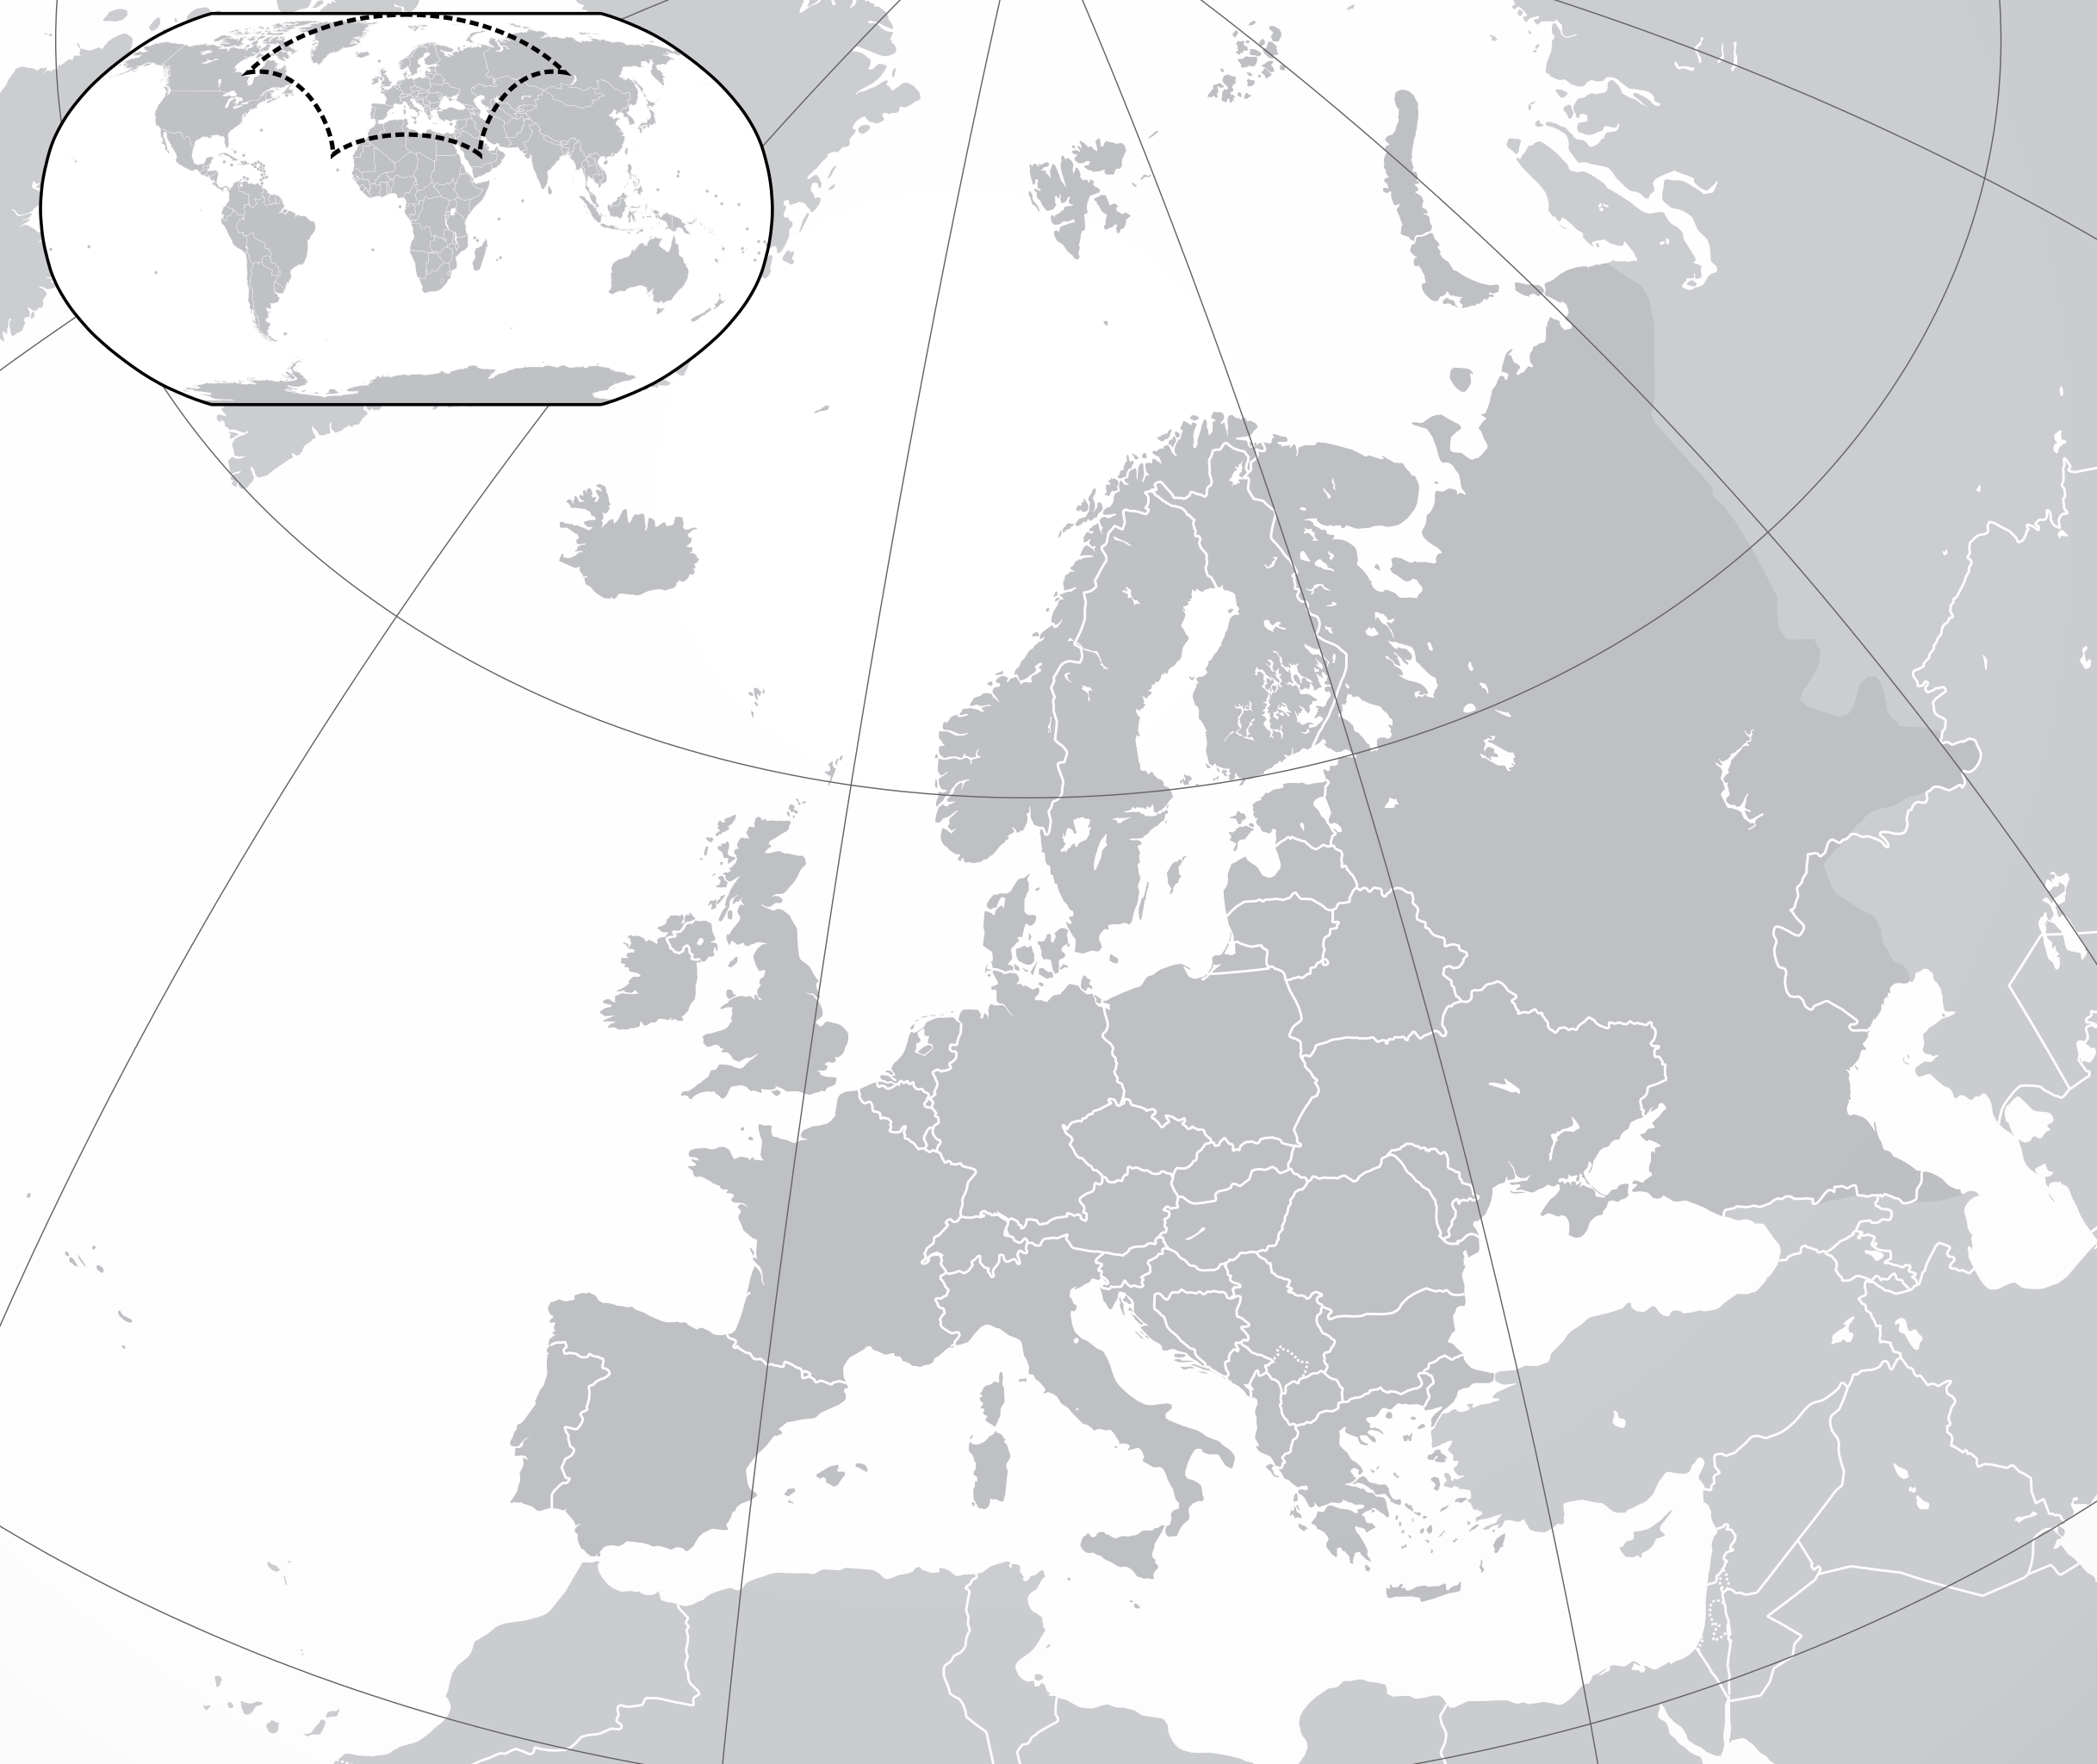
\includegraphics[width=.8\textwidth]{fig/appx/Europe-Blank.png}
    \caption{地球的局部坐标网格,图示为欧洲}
\end{figure}

\section{实流形}
物理背景作为拓扑空间,是无特征且无定形的,其中的点和曲线是不能先验识别或定义的,除非利用坐标系。有用的背景从来不可能真正脱离坐标。
坐标方法就是一种给背景点连续指定 $\R^n$ 数据的映射。
例如,平面上附着不同的坐标空间,一种可存放正交坐标,一种可存放极坐标,从而可赋予某点 $p$ 正交坐标 $(0,1)$,也可赋予极坐标 $(1,\pi/2)$,如图 \ref{fig:coor-chan}。拓扑学的同胚关系可描述坐标的指定,因为同胚具有双向连续性,且两个点不会被分配到同一坐标,从而避免歧义。
当然,同胚使得许多坐标系能力有限,不能揽下全局。比如,极坐标系不能完整覆盖 $\R^2$,坐标取值为 $V=(0,+\infty)\times(0,2\pi)$。因此常考察开子集。为圆满完成指派任务,整个背景须由若干坐标系拼接,且互相分担对方力所不及之地。

\begin{definition}
    置 $(M,\mathscr T)$。存在 $n\in\N$,使 $M$ 任意点都存在邻域同胚于 $(\R^n,\mathscr T_u)$ 某开集,则称其\textbf{局部欧的}。
    显然等价说法为:$\exists$ $M$ 的开覆盖 $\mathscr P$ 使 $\forall O\in\mathscr P$,$\exists$ 同胚 $\psi:O\to V\in\mathscr T_u$。
    $\psi$ 称为\textbf{坐标映射},$\psi(p)$ 称为 $p$ 的\textbf{坐标}。$O$ 称为\textbf{坐标域}(patch),$(O,\psi)$ 称为\textbf{坐标系}或\textbf{图}(chart)。$\mathscr P$ 所相应的坐标系族 $\mathcal A=\{(O,\psi)\}$ 称为\textbf{图册}(atlas)。$(M,\mathcal A)$ 称为\textbf{局部欧氏空间}。维数为 $\dim M:=n$。当 $\mathcal A$ 自明时简记 $M$。
\end{definition}

\begin{remark}
    同胚连续性由全集拓扑或诱导拓扑衡量。原则上可修改定义,使其允许各坐标系不同维,这样空间无唯一维数,但实用价值不大。
\end{remark}

同胚赋予的第 $i$ 个坐标构成映射 $x^i:O\to\R$,坐标系又常记 $\{x\}$。
就某个坐标系而言,坐标域的子集
    $\{p\in O: x^i(p)$ 是常函数,$i=2,\cdots,n\}$
可看成以 $x^1$ 为参数的路径,称其是一条 $x^1$ \textbf{坐标线}(coordinate line)。其它情况以此类推。全体坐标线构成\textbf{坐标网格}。
坐标域是某点邻域,故坐标系又称局部坐标系,同胚又称局部同胚。仅用一个坐标域就能覆盖则称\textbf{平凡的}(trivial),此时可称坐标系是整体坐标系。典型的例子是 $\R^n$ 自身。设 $a=(x^1_a,\cdots,x^n_a)\in\R^n$,恒等映射给出\textbf{自然坐标} $\psi(a)=(x^1(a),\cdots,x^n(a))=a$。

\begin{definition}
    第二可数 $T_2$ 的局部欧氏空间称为 \textbf{$n$ 维实拓扑流形},简记\textbf{拓扑流形} $M$。部分教材还加上仿紧的条件。将 $\R^n$ 换为 $\C^n$ 就是\textbf{复流形}。
\end{definition}

\begin{figure}[ht]
    \centering
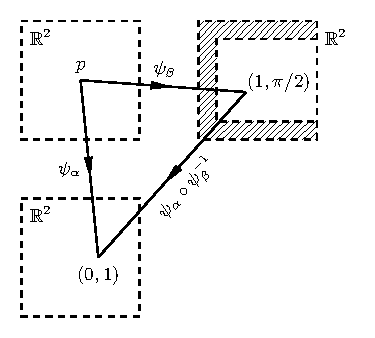
\includegraphics[width=.4\textwidth]{fig/appx/coor-chan.pdf}
    \caption{坐标变换}\label{fig:coor-chan}
\end{figure}

由于坐标域都是开的,故必存在相交之地。此处便涉及坐标系的转化。

\begin{definition}
    置某个图册 $\mathcal A$。
    取 $(O_\alpha,\psi_\alpha),(O_\beta,\psi_\beta)\in \mathcal A$ 满足 $O_\alpha\cap O_\beta\ne\mt$。
    若 $\psi_\alpha\circ\psi_\beta^{-1}$ 的 $r$ 阶导函数连续($C^r$ 性),则称它们是 $C^r$\textbf{-相容的}。$\psi_\alpha\circ\psi_\beta^{-1}$ 称为\textbf{坐标变换}或\textbf{转移函数}。
    若相交坐标系皆 $C^r$-相容,则 $\mathcal A$ 称为 $C^r$\textbf{-图册}。$C^\infty$-相容称为\textbf{光滑相容}或\textbf{相容}。
\end{definition}

\begin{remark}
    坐标变换可显式地表为 $n$ 个 $n$ 元函数,其 $C^r$ 性由 $\R^n$ 分析学给出。
\end{remark}

假设有两个图册 $\mathcal A,\mathcal B$。它们可能并不相容,即其间存在相交但不相容的坐标系。如果它们相容,则可合并为一个更大的图册。当然希望将所有相容的坐标系都囊括进来,尽可能构成足够大的图册。

\begin{definition}
    不真含于任何 $C^r$-图册的 $C^r$-图册称为\textbf{最大的}(maximal) 。若局部欧氏空间 $(M,\mathcal A)$ 的图册 $\mathcal A$ 是 $C^r$-最大图册,则称 \textbf{$C^r$-实微分流形},简称 $C^r$-流形。常考虑光滑流形。对复流形而言即要求微分结构全纯(解析)。
    最大图册又称\textbf{微分结构}。
\end{definition}

\begin{remark}
    拓扑流形是第二可数 $T_2$ 的 $C^0$-流形。实际上常默认微分流形定义中的局部欧氏空间为拓扑流形,甚至补充仿紧等性质。
\end{remark}

\begin{eg}
    \textbf{通常流形}就是指 $(\R^n,\mathscr T_u)$ 赋以包含自然坐标系的最大光滑图册。
\end{eg}

\begin{definition}
    置 $C^k$-流形上的曲线 $C$。若 $\forall p\in \Im C$,存在坐标系 $(\psi,O)$ 使 $p\in O$ 且\textbf{参数方程} $\psi\circ C$ 是 $C^r$ 的($r\leqslant k$),就称 $C$ 是 $C^r$\textbf{-曲线}。有限个光滑曲线收尾相连构成\textbf{分段光滑曲线}。
\end{definition}

\begin{remark}
    $r\leqslant k$ 使曲线 $C^r$ 性与坐标选择无关。此后类似概念的良定义性均同理。
\end{remark}

\begin{theorem}
    流形上,路径连通 $\iff$ 连通
\end{theorem}

\begin{figure}[ht]
    \centering
    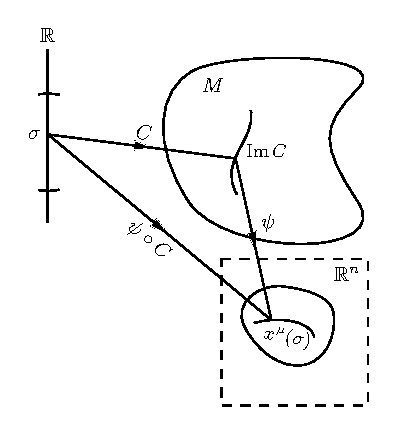
\includegraphics[width=.4\textwidth]{fig/appx/curve.pdf}
    \caption{曲线}
\end{figure}

\begin{definition}
    置 $C^k$-流形 $M,M'$。$f:M\to M'$ 称为 $C^r$\textbf{-映射},若 $\forall p\in M$,存在坐标系 $(\psi,O),(\psi',O')$ 使 $p\in O,f(p)\in O'$ 且 $\psi'\circ f\circ \psi^{-1}$ 是 $C^r$ 的($r\leqslant k$)。
    \textbf{$C^r$-微分同胚}(diffeomorphism)是双向 $C^r$ 的双射。光滑同胚的流形一定程度上可视作相等的,故又称\textbf{自同胚}。
\end{definition}
\begin{remark}
    固然希望抽象地定义 $f$,但准确定义又总要使用坐标系,通过 $\psi'\circ f\circ \psi^{-1}$ 来确定 $f$。
\end{remark}

以光滑流形为对象、光滑映射为态射,构成\textbf{光滑流形范畴} $\cate{Man}$,同构态射即光滑同胚。

考察光滑映射 $\phi:M\to N$。在 $p,\phi(p)$ 分别取坐标系 $\psi,\psi_N$,则 $\phi$ 可借助坐标系表为 $\psi_N \circ\phi\circ\psi^{-1}$。
倘若 $\phi$ 是同胚,则可定义新坐标系 $\psi':=\psi_N\circ\phi$,也即将 $\phi(p)$ 的坐标 $\psi_N(\phi(p))$ 视作 $p$ 的新坐标 $\psi'(p)$。这样给定一个 $\phi$ 相当于给定坐标变换 $\psi' \circ\psi^{-1}$。此即光滑同胚的主动、被动观点之别。

\begin{definition}
    置 $M$ 上的开覆盖 $\mathscr P=\{O_i\}$。若函数族 $\{\rho_i\}$ 满足
    \begin{itemize}
        \item $0\leqslant\rho_i\leqslant 1$;
        \item $\rho_i$ 在 $O_i$ 上光滑,且支撑在 $O_i$ 上:$x\notin O_i$ 时 $\rho_i=0$;
        \item $\sum_i \rho_i=1$,
    \end{itemize}
    则称为 $\mathscr P$ 的一个\textbf{单位分解}(partition of unity)。
\end{definition}
\begin{theorem}
    任何开覆盖均存在从属于它的单位分解。
\end{theorem}
\begin{proof}
    利用第二可数性。
\end{proof}

\section{切空间}

\begin{definition}
    流形上的函数称为\textbf{标量场}(scalar field)。置光滑流形 $M$,$U\subset M$ 上全体 $C^r$-标量场构成的集合记作 $C^r(U)$。常考虑实光滑函数。
\end{definition}

我们曾谈到矢量需要一个抽象定义。物理学的矢量总是靠作差或求导来产生,即切矢。因此可将切矢对应到曲线来定义。
给定一条穿过 $p\in M$ 的曲线 $\gamma$,要求其在 $p=\gamma(0)$ 处可导,规定给出相同切矢的曲线等价。相同性通过坐标分量($\psi\circ\gamma$ 在 $t=0$ 处导数)来判断。等价类 $[\gamma]$ 称为一个切矢。
Cartan 注意到,等价类中的曲线的沿线导数给出了相同的方向导数。例如,置 $\R^3$ 上一个可导标量场 $f$ 和曲线 $\bm r(t)$,若某点切矢为 $\bm A$,则此处 $\dv*{f}{t}=\bm{A\cdot\nabla} f$。可见,某点处的矢量总一一对应为任意标量场在该点的方向导数。数学又常常使用映射来构造概念,何不把切矢直接定义为导数本身?
可以联合矢量 $A^i$ 而构成算符 $A^i\del_i$,随后就把 $A^i\del_i$ 称为 $A$。导数映射的运算性质构造了线性空间:可相加,可数乘,还可定义零元 $0(f)=0$。这样 $\{\del_i\}$ 的确线性无关:$A=0\Rightarrow A^i=A^j\del_j(x^i)=A(x^i)=0$。因此 $\{\del_i\}$ 就是基。

标量场在此处的作用是引出切矢。犹如在电场中放入测试电荷,以静电力来研究电场自身一样,标量场受导数作用出实数,以研究导数自身,而具体的标量场不是关键。切矢和偏导的关系,就类似于电场和静电力的关系。

通常会采取更抽象但更优雅的定义。考察若干等价性质,这样能脱离分量而直接给出切矢整体。注意基源自各坐标偏导,$f$ 有 $n$ 个独立的求导方向,而若 $f\circ\psi^{-1}$ 是 $n$ 元的光滑函数,可用 $x^i$ 展开为
\[
    f=f(p)+\del_i f(p)(x^i-x^i(p))+ \frac 12\del_i\del_j f(p)(x^i-x^i(p))(x^j-x^j(p))+\cdots.
\]
$A$作用于它只剩下 $A(f)=A(x^i)\del_i f(p)=:A^i\del_i f(p)$,高阶项为零是因为必然存在 $x^j(p)-x^j(p)=0$。该过程只用到导数算子的线性性和 Leibniz 乘法法则(二者可推出常函数导数为零),故可认为\textit{一点处的切矢是满足 Leibniz 乘法法则的线性泛函}。
当然,对无穷级数滥用代数性质是极为危险的,我们更倾向于考虑有限项相加,其次不一定要求标量场光滑。
总之 Cartan 体系里所有东西都是泛函或算符,甚至是更多层嵌套。

这说明切矢定义在线性空间乃至一个代数上。就 $C^r(M)$ 而言这比较好办,只需规定运算使 $\forall p\in M,f,g\in C^r(M)$,
\eq{(f+g)(p):=f(p)+g(p),\quad  (fg)(p):=f(p)g(p),}
且将常函数的赋值 $\alpha\in\R$ 就记为函数名,即 $\alpha(p):=\alpha$,数乘即用常函数相乘。光滑性使运算封闭。$C^r(M)$ 构成交换幺环,称为\textbf{光滑函数环}。但由于非零元不一定有逆,因此不能构成域:设 $f\ne 0$ 但存在零点,则不存在 $g$ 使 $f(p)g(p)=1$ 恒成立。同时 $C^r(M)$ 也是 $\R$-模,结合环性有 $\alpha(fg)=(\alpha f) g=f(\alpha g)$,构成 $\R$-代数。
然而,在给出坐标分量时用到了某坐标系 $(\psi,O)$ 和 $x^i\in C^k(O)\ne C^k(M)$。可见,我们要考虑的是如何给 $C^r(O)$ 构造线性性。

$C^k(M)$ 是合法的





我们如何合法地谈及 $A(x^i)$ 呢?将 $x^i$ 任意拓展到 $M$ 上即可,因为只要 $f_1,f_2\in C^r(M)$ 在 $U\in\mathscr N(p)$ 上相等,则 $p$ 点任意切矢 $A$ 满足 $A(f_1)=A(f_2)$。对此只需置 $f:=f_1-f_2$ 并证明 $A(f)=0$。令 $h$ 在 $M\backslash U$ 上为零但 $h(p)\ne 0$,就可构造零元 $fh=0$,则 $0=A(fh)=h(p)A(f)$ 从而 $A(f)=0$。

\begin{definition}
    置流形 $M$。设 $V\subset U\subset M$。$f:V\to\R$ 称为 $g:U\to\R$ 在 $V$ 上的\textbf{限制},若 $\forall p\in V,f(p)=g(p)$。显然限制是唯一的。$g$ 称为 $f$ 在 $U$ 上的一个\textbf{延拓}。

    
\end{definition}

对光滑流形 $M$ 及 $p\in M$,在 $C^r(M)$ 中规定等价关系:存在 $N\in\mathscr N(p)$ 使 $f,g\in C^r(M)$ 在 $N$ 上的限制相同。等价类 $[f]$ 称为\textbf{函数芽},构成 $C^r(M)$ 的商集 $\mathscr G_p$。
    \eq{
        [f]+[g]:=[f+g],\quad [f][g]:=[fg].
    }
\begin{definition}
    $p\in M$ 处的\textbf{切矢} $v$ 是 $\mathscr G_p$ 上的线性函数,且 $\forall f,g\in\mathscr G_p$
    \eq{
        v(fg)=g(p)v(f)+f(p)v(g).
    }

    $p$ 处全体切矢的集合 $T_p M$ 称为 $M$ 在 $p$ 处的\textbf{切空间}。全体切空间的无交并
    \eq{
        TM:=\bigsqcup_{p\in M} T_p M=\bigcup_{p\in M}\{p\}\times T_p M=\{(p,v):p\in M,v\in T_p M\}
    }
    称为\textbf{切丛}(tangent bundle)。
\end{definition}

\begin{remark}
    部分教材将无交并写作 $\coprod$。
    直观图像是把切空间理解为背景在该点的切平面。
\end{remark}


\begin{theorem}
    $\dim T_p M=\dim M$。
\end{theorem}

\begin{proof}
    总存在光滑标量场 $H_i$ 使得 $f(q) =f(p)+(x^i(q)-x^i(p))H_i(q)$,只需定义
\eq{
    H_i(q):=\left\{\begin{aligned}
        \frac{f(q)-f(p)}{x^i(q)-x^i(p)},&\quad q\ne p.\\
        \pdv{(f\circ\psi^{-1})}{x^i}\bigg|_{\psi(p)},&\quad q=p.
    \end{aligned}\right.
}
现在大可使用线性性和 Leibniz 乘法法则,得到 $A(f)=H_i(p) A(x^i)$,故总存在 $n$ 个实数 $\{A(x^i)\}$,只要记
\eq{
A^i:=A(x^i),
}
就有
\eq{
    A(f):=A^i\pdv{(f\circ\psi^{-1})}{x^i}\bigg|_{\psi(p)},
}
\end{proof}

$X_\mu$

\begin{definition}
    $X_i$ 称为 $p$ 处第 $i$ 个\textbf{坐标基矢}。$\{X_i\}$ 称为 $p$ 处的\textbf{坐标基}。
\end{definition}

\begin{theorem}
    利用映射语言给出切矢的分量变换律。
\end{theorem}
\begin{proof}只需注意
    \[
    X_i(f)=\pdv{(f\circ\psi^{-1})}{x^i}\bigg|_{\psi(p)}=\pdv{x'^j}{x^i}\bigg|_{\psi(p)}\pdv{(f\circ\psi'^{-1})}{x'^j}\bigg|_{\psi'(p)}={\pdv{x'^j}{x^i}}(p)X'_j(f),
    \]
其中 $\pdv*{x'^j}{x^i}$ 是标量场。
\end{proof}

\begin{definition}
    $T^*_p M:=(T_p M)^*$ 称为 $M$ 在 $p$ 处的\textbf{余切空间},其元素称为 $M$ 在 $p$ 处的\textbf{余切矢}。
    全体余切空间的无交并 $T^*M:=\bigsqcup_{p\in M} T^*_p=\{(p,\omega):p\in M,\omega\in T^*_p M\}$ 称为\textbf{余切丛}。
\end{definition}

代入 $V=T_p M,e_i=X_i$ 即可得到分量变换律。
\eq{
    T=T^{\mu_1\cdots\mu_k}{}_{\nu_1\cdots\nu_l}\partial_{\mu_1}\otimes\cdots\otimes\partial_{\mu_k}\otimes\d x^{\nu_1}\otimes\cdots\otimes\d x^{\nu_l}.
}

余切矢量场和切矢场的缩并其实就是将对偶矢量作用于矢量,即
$\langle \omega, v\rangle$。

\section{张量场}

切矢场就是给流形各处指定一个切矢,准确而言,还要带上起点信息:
\begin{definition}
    置 $U\subset M$。映射 $v:U\to TM$ 称为 $U$  上的\textbf{切矢场},$\Im v$ 称为 $TM$ 在 $U$ 的一个\textbf{截面}(section)。
\end{definition}

\begin{definition}
    置 $C^1$-曲线 $\sigma\mapsto C(\sigma)$ 的\textbf{曲线切矢场}
\eq{
\dv{\sigma} (f)=\dv{(f \circ C)}{\sigma},
}
\end{definition}

\begin{eg}
    第 $x^i$ 坐标线的切矢正是坐标基 $\delta^j_i\del_j=\del_i$。
\end{eg}

\begin{theorem}
    \eq{\dv{\sigma}=\dv{(x^i \circ C)}{\sigma}\del_i.}
\end{theorem}

借助于至少囊括曲线段的坐标系 $\{x^\mu\}$,则 $x^\mu$ 在曲线上关于 $[t_1,t_2]$ 分段可导,故 $\dv*{t}$ 可展开至坐标基
    \[\dv{t}=\dv{x^\mu}{t}\pdv{x^\mu},\]

曲面

\[
        \pdv{t}=\pdv{x^\mu}{t}\pdv{x^\mu},
    \]
    故应记 $\partial_t$。

置映射 $g:A\to A$ 和 $f:A\to A$。若 $f\circ g=g\circ f$,则称 $f,g$ 是\textbf{对易的}(commutative)。若 $A$ 有减法运算,称映射 $[f,g]$ 为 $f,g$ 的\textbf{对易子}(commutator),使 $[f,g](x)=f(g(x))-g(f(x))$。$f,g$ 对易即 $[f,g](x)=0$,简写为 $[f,g]=0$。、

矢量场可导指矢量场按任意坐标基展开的分量为坐标域上的可导函数。

光滑性

\begin{definition}
    \textbf{对易子}(commutator),使 $[f,g](x)=f(g(x))-g(f(x))$。
\end{definition}


\begin{theorem}
    光滑矢量场对易子 $[A,B]$ 仍是光滑矢量场。
\end{theorem}
\begin{proof}
    映射语言上显然。分量语言上,注意 $v(f)$ 在坐标基下等于 $v^\mu\partial_\mu f$,故对易子即
    \eq{
        [A,B]^\lambda=A^\mu\partial_\mu B^\lambda-B^\mu\partial_\mu A^\lambda.
    }
    应证它满足张量变换式:
    \[
        \pdv{x^\sigma}(\pdv{x'^\lambda}{x^\kappa}B^\kappa)=  B^\kappa\pdv{x'^\lambda}{x^\sigma}{x^\kappa}+\pdv{x'^\lambda}{x^\kappa}\partial_\sigma B^\kappa,
    \]
    因为 $\partial_\sigma\partial_\kappa=\partial_\kappa\partial_\sigma$ 始终使 $\pdv{x'^\lambda}{x^\sigma}{x^\kappa}$ 项抵消。
\end{proof}

\begin{eg}
    Fubini 定理指出 $\left[\del_\mu,\del_\nu\right]=0$,又称\textbf{偏导对易性}。
\end{eg}


Cartan 还注意到余切空间可给函数微分一个更严格的理解。标准分析学中常将 $\d f$ 定义为 $\Delta f$ 的线性主部,即 $\d f(x,\Delta x):=f'(x)\Delta x$。物理上的理解是在 $\Delta x$ 很小时给出的微小增量。由于 $\Delta x$ 是从某点 $x$ 出发的微小位移,因此一个更合适的理解是切矢,即
\eq{
    \d f(p)(A):=A(f)=A^i\del_i f.
}
可以看到 $x^i$ 的微分正是坐标基 $\del_i$ 的对偶 $\d x^i(\del_j)=\del_j(x^i)=\delta^i_j$,称为\textbf{对偶坐标基}或\textbf{逆变基}。故 $\d f$ 的分量是 $\d f(\del_i)=\del_i f$,即可展开为 $\d f=\del_i f \d x^i$。在标准分析中,全微分理解为各线性映射间的关系,这里将线性映射叙述为余切矢量。由于分量是 $\del_i f$,因此有时建议称标量场的\textbf{梯度}\footnote{为区分于标准分析学中的概念,部分书籍会用粗体表示这些泛函,如 $\bm A,\bm\omega,\bm{\del}/{\bm{\del}x^i},\bm{\d}f$。但其实没有必要,因为两种概念其实是一致的。看似不同是因为本科教学为了通俗性,默认以坐标空间为基础,而没有额外提出流形。}。

函数的微分,对于标量函数有这些运算:加法 $f+g$、乘法 $fg$ 和微分 $f\mapsto\text df$。乘法对于加法是可分配的。微分对乘法也是一个分配,即 Leibniz 法则。

流形上的度规场是指在切丛上指定度规。

借此定义切空间元素的内积、正交性、模长、正交归一性。度规在正交归一基的分量一定是对角归一矩阵,其迹称为号差。号差将度规分为正定(Riemann 的)、负定和不定。非正定就称伪 Riemann 的。只有一个对角元符号不同的不定度规称 Lorentz 的。对 4 维情况,号差为 $\pm 2$。按号差 $+2$ 的习惯,一般定义 $\eta_{\mu\nu}$ 为 $\diag(-1,1,1,1)$ 的矩阵元。推广到切丛上,度规场除对称、处处非退化外,还要求号差处处一致。显然度规场的号差与坐标系选择无关。类比线性代数的合同变换,可见总存在坐标系使其分量矩阵为对角归一矩阵。

正定度规称为\textbf{Riemann 的}。

固有时需要将切空间的模长概念搬到切丛上来

单位分解搬到时空上来。

\begin{definition}
    分段 $C^1$-曲线 $C:[t_1,t_2]\to M$

线长是其上 Riemann 积分泛函(或视作 $\Im C$ 的 Lebesgue 测度)
    \[L(C)=\int_{t_1}^{t_2} \sqrt{\abs{g\left(\dv{t},\dv{t}\right)}}\d{t},\]

    这里 $\dv*{t}$ 表示曲线按 $t$ 参数化时的切矢场。
\end{definition}

\begin{theorem}
    线长与参数选择无关。
\end{theorem}

\begin{remark}
    但没排除
    一部分使 $\dv*{t}$ 为零元的情形,但还应要求 $[t_1,t_2]$ 中不能有 Lebesgue 测度大于零的区间使像点 $C(t)$ 一致。
    
    测度为零区间是允许的,如 $t$ 的鞍点或曲线自交的情形。
\end{remark}
    
    则很容易发现的形式写法为
    \[
        L(C)=\int_C \sqrt{\abs{g_{\mu\nu}\d x^\mu\d x^\nu}}.
    \]
    因此可引入形式记号 $\d s^2=g_{\mu\nu}\d x^\mu\d x^\nu$ 而不论及线元 $\d s$ 的“虚实性”。此外,很容易发现参数单调性还迎合了物理学的因果要求。
    
即它是两个矢量的线性函数 $g:V\times V\to\R$。首先有对称性 $g(A,B)=g(B,A)$;其次,若 $\forall B\in V$ 都有 $g(A,B)=0$,我们希望这只在 $A=0$ 时才能发生。这称为\textbf{非退化性}。规定度规的坐标分量是 $g_{ij}:=g(\del_i,\del_j)$,这样立即得出了。这样 $g_{ij}$ 可以看成 $g$ 在某坐标系下具体表达出的若干实数,$(g_{ij})$ 是 $g$ 的一个分量矩阵,且是对称的:
 $g_{ij}=g_{ji}$。内积的分量写法是 $g( A, B)=g_{\mu\nu} A^\mu B^\nu$。
 
 这样曲线 $C(\sigma)$ 上任意两点间的线长就可定义为
 \eq{
    \l:=\int_C\bigg|g\left(\dv{\sigma},\dv{\sigma}\right)\bigg|^{1/2}\d\sigma,
 }
 显然,仿射参数使切矢模方恒定,而线长参数还将使其归一为 $g(\dv{\sigma},\dv{\sigma})=\pm 1$。

 这样正交归一系的坐标基就是使 $g(\del_i,\del_j)=\tilde g_{ij}$。

度规可以展开成线性组合,这涉及从矢量的基底构造一种新基底,将运算符记作 $\otimes$,并期望度规能表示成 $g=g_{ij}\d x^i\otimes\d x^j$。为寻找其合理定义,尝试两边作用于切矢,则式左是 $g_{ij}A^i B^j=g_{ij} \d x^i(A)\d x^j(B)$,式右是 $g_{ij}\d x^i\otimes\d x^j(A,B)$,故直接希望 
$\d x^i\otimes\d x^j(A,B):=\d x^i(A)\d x^j(B)$,即 $\otimes$ 的结果与相应矢量的作用相当于各自分开作用再相乘。

即 $A\otimes B(\omega_1,\omega_2):=A(\omega_1)B(\omega_2)$,这样 的分量是只是简单拼凑 $A^i B^j$。

给背景每一点指定一个度规就形成了\textbf{度规场}。总需先借助一个坐标系才能说清度规分量的定义,比如欧氏度规可用自然坐标系写作 $\delta=\delta_{ij}\d x^i\otimes\d x^j$,而闵氏度规是 $\eta=\eta_{\mu\nu}\d x^\mu\otimes\d x^\nu$。\textbf{欧氏空间} $\mathbb{E}^n$ 就是 $\R^n$ 配以欧氏度规,记法上可将二者打包成 $(\R^n,\delta)$。\textbf{闵氏时空}就是 $\R^{1,3}:=(\R^4,\eta)$。

4-速的 Cartan 写法是 $U:=\dv*{\tau}$。 

Lorentz 坐标系。

Descartes 坐标系可包括自然坐标系及其平移、旋转。

同理,惯性坐标系可包括自然坐标系的平移或“旋转”,用 矩阵 $\Lambda$ 描述“旋转”的部分,换言之,就是使得 $\Lambda$ 为正交矩阵的仿射变换。

由 $\R^4$ 的线元不变性,可严格导出变换的仿射性,便绕过了对各种“公设”的争辩:

已经证明过$\R^4$ 上的任意两个惯性坐标系间的变换仿射。



\begin{definition}
    流形上的形式场称为\textbf{微分形式}(场)。常取对偶坐标基将 $l$-微分形式 $\omega$ 表为
    \eq{
    \omega=\sum_{\mu_1<\cdots<\mu_l}\omega_{\mu_1\cdots\mu_l} \d x^{\mu_1}\wedge\cdots\wedge \d x^{\mu_l}=\frac{1}{l!}\omega_{\mu_1\cdots\mu_l} \d x^{\mu_1}\wedge\cdots\wedge \d x^{\mu_l}.
    }
    连续的非零张量场称\textbf{非退化的}。非退化最高阶形式场称\textbf{体元场}或\textbf{体元}。
\end{definition}

\begin{definition}
    存在体元的流形称\textbf{可定向的}(orientable)。
\end{definition}

    \begin{eg}
        $\R^3$ 可定向:只需取自然坐标便知存在光滑体元 $\d x\wedge\d y\wedge\d z$。
    \end{eg}
    \begin{eg}
    M\"obius 环(图 \ref{mobius})不可定向:若尝试连续指定非零定向,则沿途回到原处时一定会断开,而突然反号不满足连续要求。直观上讲这意味着它作为 2 维曲面却只有一个面,不能区分正反。
    \end{eg}

\begin{definition}
    类似地,对体元场 $\epsilon_1,\epsilon_2$,若存在标量场 $h>0$ 使 $\epsilon_1=h\epsilon_2$,就说 $\epsilon_1,\epsilon_2$ 等价,由此体元场的等价类称为该流形的定向。
    选好定向的可定向流形称(已)\textbf{定向的}(oriented),类似地有正定体元、右手基等概念。
    若坐标系的坐标基是右手的,则称\textbf{右手系}。
\end{definition}

\begin{figure}[h!]
    \centering
\tikzset{every picture/.style={line width=0.75pt}} %set default line width to 0.75pt        

\begin{tikzpicture}[x=0.75pt,y=0.75pt,yscale=1,xscale=1]
%uncomment if require: \path (0,300); %set diagram left start at 0, and has height of 300

%Curve Lines [id:da7826517172347827] 
\draw    (3.65,18.88) .. controls (17.2,36.58) and (48,50.16) .. (72.8,51.99) ;
\draw [shift={(39.71,43.88)}, rotate = 205.45] [fill={rgb, 255:red, 0; green, 0; blue, 0 }  ][line width=0.08]  [draw opacity=0] (8.4,-2.1) -- (0,0) -- (8.4,2.1) -- cycle    ;
%Curve Lines [id:da8566552148207576] 
\draw    (221.73,12.59) .. controls (241.17,-1.67) and (128.44,8) .. (140.66,18.19) ;
%Curve Lines [id:da14270801999584393] 
\draw  [dash pattern={on 3pt off 3pt on 3pt off 3pt}]  (183.2,21.91) .. controls (174,25.58) and (149.2,26.68) .. (140.66,18.19) ;
%Curve Lines [id:da5926224666835718] 
\draw  [dash pattern={on 3pt off 3pt on 3pt off 3pt}]  (221.73,12.59) .. controls (206.74,22.26) and (214.4,6.87) .. (183.2,21.91) ;
%Curve Lines [id:da4918795365326445] 
\draw    (223.95,9.53) .. controls (217.84,52.82) and (166.2,65.55) .. (140.66,18.19) ;
%Straight Lines [id:da406966878688231] 
\draw    (163.2,42.45) -- (149.8,65.67) ;
\draw [shift={(148.8,67.4)}, rotate = 299.99] [fill={rgb, 255:red, 0; green, 0; blue, 0 }  ][line width=0.08]  [draw opacity=0] (7.2,-1.8) -- (0,0) -- (7.2,1.8) -- cycle    ;

\end{tikzpicture}
    \caption{曲线、曲面的定向}
\end{figure}

\section{带边流形}

现借助坐标系叙述之。在 $M$ 中有一包含 $p$ 的局部坐标系 $(O,\psi;x^i)$,使得 $\psi(p)$ 是坐标原点且 $U\cap D =\{q\in U|x^1(q)\leqslant 0\}$,则称 $D$ 是 $M$ 上的一个\textit{带边区域},其边界点 $x^1$ 坐标为零。坐标空间里这个区域就称作“\textit{半空间(half-space)}” $\mathbb H^{n}$,有时可记作 $\frac{1}{2}\R^n$。由于边界点失去了一个坐标自由度,因此我们很容易发现 $\partial D$ 是相较于 $D$ 而言“余 1 维(1-codimension)”。考虑到背景和内部都是同维开集,因此说\textit{带边区域不能直接认同为普通开集},因其在实质上“强行”拼凑了两个不同维度的东西,即内部和边界。

区域定向可在其边界上也诱导出与之相应的定向

\begin{figure}[h!]
    \centering
\tikzset{
pattern size/.store in=\mcSize, 
pattern size = 5pt,
pattern thickness/.store in=\mcThickness, 
pattern thickness = 0.3pt,
pattern radius/.store in=\mcRadius, 
pattern radius = 1pt}
\makeatletter
\pgfutil@ifundefined{pgf@pattern@name@_hask52a3i}{
\pgfdeclarepatternformonly[\mcThickness,\mcSize]{_hask52a3i}
{\pgfqpoint{0pt}{0pt}}
{\pgfpoint{\mcSize+\mcThickness}{\mcSize+\mcThickness}}
{\pgfpoint{\mcSize}{\mcSize}}
{
\pgfsetcolor{\tikz@pattern@color}
\pgfsetlinewidth{\mcThickness}
\pgfpathmoveto{\pgfqpoint{0pt}{0pt}}
\pgfpathlineto{\pgfpoint{\mcSize+\mcThickness}{\mcSize+\mcThickness}}
\pgfusepath{stroke}
}}
\makeatother

% Pattern Info
 
\tikzset{
pattern size/.store in=\mcSize, 
pattern size = 5pt,
pattern thickness/.store in=\mcThickness, 
pattern thickness = 0.3pt,
pattern radius/.store in=\mcRadius, 
pattern radius = 1pt}
\makeatletter
\pgfutil@ifundefined{pgf@pattern@name@_9v4tzcn4d}{
\pgfdeclarepatternformonly[\mcThickness,\mcSize]{_9v4tzcn4d}
{\pgfqpoint{0pt}{0pt}}
{\pgfpoint{\mcSize+\mcThickness}{\mcSize+\mcThickness}}
{\pgfpoint{\mcSize}{\mcSize}}
{
\pgfsetcolor{\tikz@pattern@color}
\pgfsetlinewidth{\mcThickness}
\pgfpathmoveto{\pgfqpoint{0pt}{0pt}}
\pgfpathlineto{\pgfpoint{\mcSize+\mcThickness}{\mcSize+\mcThickness}}
\pgfusepath{stroke}
}}
\makeatother
\tikzset{every picture/.style={line width=0.75pt}} %set default line width to 0.75pt        

\begin{tikzpicture}[x=0.75pt,y=0.75pt,yscale=1,xscale=1]
%uncomment if require: \path (0,300); %set diagram left start at 0, and has height of 300

%Shape: Polygon Curved [id:ds6324304927731197] 
\draw   (14,85) .. controls (10,122) and (65.25,88.75) .. (74.25,80.25) .. controls (83.25,71.75) and (88.25,58.25) .. (81.25,45.25) .. controls (74.25,32.25) and (36.25,-5.25) .. (16.25,24.75) .. controls (-3.75,54.75) and (18,48) .. (14,85) -- cycle ;
%Shape: Rectangle [id:dp42790425123431874] 
\draw  [dash pattern={on 4.5pt off 4.5pt}] (142,117) node[below right]{$\mathbb H^n$} -- (252,117)node[below right]{$\R^n$} -- (252,7) -- (142,7) -- cycle ;
%Straight Lines [id:da2780621449052143] 
\draw    (197,117) -- (197,7) ;
%Curve Lines [id:da11211326883897499] 
\draw [pattern=_hask52a3i,pattern size=6pt,pattern thickness=0.75pt,pattern radius=0pt, pattern color={rgb, 255:red, 0; green, 0; blue, 0}] [dash pattern={on 4.5pt off 4.5pt}]  (197,25) .. controls (167,52) and (161,80) .. (196,97) ;
%Shape: Polygon Curved [id:ds6020575675206878] 
\draw  [pattern=_9v4tzcn4d,pattern size=6pt,pattern thickness=0.75pt,pattern radius=0pt, pattern color={rgb, 255:red, 0; green, 0; blue, 0}][dash pattern={on 4.5pt off 4.5pt}] (57.25,56.75) .. controls (55.75,74.75) and (65.25,88.75) .. (74.25,80.25) .. controls (83.25,71.75) and (88.25,58.25) .. (81.25,45.25) .. controls (74.25,32.25) and (58.75,38.75) .. (57.25,56.75) -- cycle ;
%Curve Lines [id:da8087172400108391] 
\draw [line width=0.75]    (77.25,67.75) .. controls (119.39,104.75) and (169.21,96.84) .. (192.37,74.39) node[near start,sloped,above]{$\psi$};
\draw [shift={(193.75,73)}, rotate = 133.75] [fill={rgb, 255:red, 0; green, 0; blue, 0 }  ][line width=0.08]  [draw opacity=0] (8.4,-2.1) -- (0,0) -- (8.4,2.1) -- cycle    ;
\end{tikzpicture}
    \caption{带边区域}
\end{figure}

\section{超曲面}


\begin{definition}[切矢和法矢]
    设 $S$ 是背景 $M$ 上可具有不同维度的子集。将 $S$ 上一点 $q$ 处的矢量称为切矢 $w$,若 $S$ 上存在过 $q$ 的曲线与其相切。用坐标基易验证,$q$ 处所有矢量构成的矢量空间 $V_q$ 与 $M$ 同维,而所有 $w$ 所构成的集合称作切空间,记作 $T_q S$,是 $V_q$ 的矢量子空间。

    可以定义 $q$ 处的法矢 $n$,若对任意切矢 $w$ 有 $\langle n,w\rangle=0$,这里内积取决于 $M$ 所选度规。
\end{definition}
\begin{theorem}
    当 $S$ 是 $M$ 的余 1 维子空间时,又可以形象地叫做一张\textbf{超曲面}(hypersurface),其上一点的任意法矢间只差倍数关系。
\end{theorem}


\begin{proof}
    证明 设 $\left\{e_2, \cdots,e_n\right\}$ 为 $T_q S$ 任一坐标基, 因 $\dim V_q=n, V_q$ 必有与 $\left\{e_2,\cdots,e_n\right\}$ 线性无关的元素, 任取其一并记作 $e_1$, 则 $\left\{e_\mu\mid\mu=1, \cdots, n\right\}$ 为 $V_q$ 的基底。令 $n=e_1$, 则 $\langle n, e_\tau\rangle =g(e_1,e_\tau)=0$,这里 $\tau=2,\cdots,n$,可见 $n$ 为法矢。若存在 $m$ 满足 $\langle m,e_\tau\rangle=0$, 则其在 $\left\{e_\mu\right\}$ 的分量 $m^\tau=0$, 因而只剩下分量 $m^1$,即 $m=m^1\left(e_1\right)^a$ $=m^1n$, 即 $m$ 与 $n$ 只差一因子 $m^1$。
\end{proof}
注意,余维数太多的话,比如三维空间的曲线,其上法矢就没有该性质了,因此选取更为任意。对于超曲面,约定其模长可以使得差别仅体现在“内外方向”上。以后默认取单位法矢,即要求 $\langle n,n\rangle=\pm 1$,正负号来自度规的正负定性。设 $p\in S$ 上的一个局部坐标系 $(U;x^1,\cdots,x^{n})$ 是 $M$ 正定的右手系使得域内点 $x^n\leqslant 0$,则$(U\cap S;x^1,\cdots,x^{n-1})$ 也是 $S$ 的局部坐标系,且 $\pdv{x^n}$ 就是法矢而且是外法矢。

对一点 $q$,度规的作用范围是其整个矢量空间 $V_q$,因此类似于切矢,度规也有“切于” $S$ 的部分,那就是只作用于 $T_qS$ 的部分。


此外,任意 $l$-形式也能按相应思路定义其\textbf{诱导形式},这是有必要的,因为一旦把 $S$ 看作一个独立区域,而非从背景的嵌入视角观察,那么“不切于”的形式都是没有意义的。
体元、定向也是形式,自然也有其诱导。

\begin{definition}[诱导度规]
    设 $S$ 是背景 $M$ 的子集而别无他求,其上一点 $q$ 处的切空间 $T_q S$ 的度规 $\tilde g$ 称为 $V_q$ 上 $g$ 的诱导度规(induced metric),若对任意 $w_1,w_2\in T_q S$ 有
    \eq{\tilde g(w_1,w_2)=g(w_1,w_2),}
    可见诱导度规只是将度规的作用对象从 $V_q$ 限制于 $T_q S$,因此又称作度规在 $S$ 上的限制(restriction)。$g$ 定义在 $V_q$ 上,而 $\tilde g$ 可视作定义在$T_q S$ 上。
\end{definition}
满足上式的诱导度规有很多,下面介绍一种用于超曲面的惯例。在规定其单位法矢后,将 $v$ 沿着法向和切向分解,可得垂直的 $v_n=\pm\langle v,n\rangle n$(正负跟随 $\langle n,n\rangle=\pm 1$),切向就是 $v_t=v-v_n$,即
\[
v=v_t\pm\langle v,n\rangle n,
\]
如果将 $v_t$ 视作 $v$ 的\textit{投影(projection)}或限制,则应当有 (1,1) 型张量 $h$ 满足 $v_t=\c_1^2(h\otimes v)$,即
\[
v_t=h(\oo;v)=v\mp  n_\flat(v)n=I(\oo;v)\mp  n\otimes n_\flat(\oo;v),
\]
说明 $h=I\mp  n\otimes n_\flat$,用 $g$ 降下来,
\eq{
h_\flat=\c_1^1(g\otimes I)\mp \c_1^1(g\otimes n\otimes n_\flat)=g\mp n_\flat\otimes n_\flat,
}
可以验证这就是一个诱导度规。下面从缩并角度解释其合理性。为便于陈述, 设 $V_q$ 为 4 维,因而 $T_q S$ 为 3 维。作为诱导度规,$\tilde g$ 是 $T_q S$ 上的 3 维张量,即 $\tilde g \in \mathscr{T}_{T_q S}(0,2)$ (它不能作用于 $V_q\backslash T_q S$ 的元素)。但为了便于用 4 维等式演算,我们希望找到一个 4 维的 $(0,2)$ 型张量(即 $\mathscr{T}_{V_q}(0,2)$ 的元素),它能代表 3 维张量 $\tilde g$。而 $h_\flat \equiv g \mp n_\flat\otimes n_\flat$ 就是这样的 4 维张量等式。可以证明 $\mathscr{T}_{V_q}(0,2)$ 的子集 $\mathscr{S}_{V_q}(0,2) \equiv\left\{T \in\right.$ $\left.\mathscr{T}_{V_q}(0,2) \mid T( n,\oo)=0,T(\oo,n)=0\right\}$ 与 $\mathscr{T}_{T_q S}(0,2)$ 自然同构,因而可作认同\footnote{详见第 3 章参考系一节。}。

易见 $g \notin \mathscr{S}_{V_q}(0,2)$ 而 $h_\flat \in \mathscr{S}_{V_q}(0,2)$ ,且 $h_\flat(w_1,w_2)=g (w_1,w_2),\forall w_1,w_2\in T_q S$,所以可把 $h_\flat$ 认同为 $\tilde g$。容易验证 $\mathscr{S}_{V_q}(0,2)$ 中满足诱导度规定义(因而可充当 $\tilde g$)的元素只有 $h_\flat$,这就是把 4 维张量 $h_\flat \equiv g \mp n_\flat\otimes n_\flat$ 看作诱导度规的理 由。以后将不在符号上区分 $h_\flat$ 和 $\tilde g$.

以上关于 $(0,2)$ 型张量的结论还可推广:由 $T\in \mathscr{T}_{V_q}(0,k)$ 满足其任意槽与 $n$ 缩并为零,所构成的集合与 $\mathscr{T}_{T_q S}(0, l)$ 有自然同构关系。这使我们在讨论和书写公式时可用前者的元素代替后者的元素(写成 4 维而非 3 维张量等式),从而带来许多方便。
   % 流形
        \chapter{仿射联络及曲率}\label{appx:curvature}
\begin{definition}
    置 $C^{h}$-流形 $M$。
    \textbf{仿射联络}或\textbf{协变微分}是将 $(k,l)$ 型 $C^{r+1}$-张量场映为 $(k,l+1)$ 型 $C^{r}$-张量场($h\geqslant r+2$)的线性算符 $\nabla$,满足:对张量积有 Leibniz 乘法法则;与缩并对易;对 $C^1$-函数 $f$ 有 $\nabla f=\d f$。分量记作 $\nabla_\mu T^{\cdots}_{\cdots}$,算符 $\nabla_\mu$ 称为\textbf{协变导数}。$\nabla_X:=\c^1_1(X\otimes\nabla)$ 称为沿矢量场 $X$ 的\textbf{方向导数}。$(M,\nabla)$ 构成\textbf{联络空间}。
\end{definition}

\begin{eg}
    对标量场 $f$,$\nabla_X f=\langle\d f,X\rangle=X(f)$。
\end{eg}


\begin{definition}
    置联络空间 $(M,\nabla)$ 和矢量基场 $\{e_\mu\}$,\textbf{联络系数}为 $\Gamma^\lambda_{\mu\nu}:=\langle e^\lambda,\nabla_{e_\mu} e_\nu\rangle$。
    $\Gamma^\lambda_\nu:=\Gamma^\lambda_{\mu\nu} e^\mu$ 称为\textbf{联络 1-形式}。
\end{definition}

\begin{remark}
    一律建议将联络系数定义为分量形式,以避免讨论其张量性等无伤大雅的问题。
\end{remark}

\begin{theorem}
    $\nabla e_\nu=\Gamma^\lambda_\nu\otimes e_\lambda.$
\end{theorem}

\begin{theorem}
    置对矢量场 $Y$ 和坐标系 $\{x\}$。$\nabla Y$ 坐标分量为 $\nabla_\mu Y^\lambda=\del_\mu Y^\lambda+\Gamma^\lambda_{\mu\nu}Y^\nu$。
\end{theorem}
\begin{remark}
    务必注意 $\Gamma^\lambda_{\mu\nu}Y^\nu$ 的缩并顺序。
\end{remark}
\begin{proof}置 $\{e_\mu\}$,则
    \[\nabla(Y^\nu e_\nu)=\d Y^\nu\otimes e_\nu+Y^\nu \Gamma^\lambda_{\mu\nu} e^\mu\otimes e_\lambda=\del_\mu Y^\lambda\d x^\mu\otimes e_\lambda+Y^\nu \Gamma^\lambda_{\mu\nu} e^\mu\otimes e_\lambda,\]
    取 $e_\mu=\del_\mu$ 即可。
\end{proof}

\begin{theorem}
    设 $e_\mu^{\prime}=A^\nu{ }_\mu e_\nu$,则
    \begin{align*}
        \Gamma'^{\gamma}_{\sigma\kappa}&=\langle e'^\gamma,\nabla_{e'_\sigma} e'_\kappa\rangle=(A^{-1})^\gamma{}_\lambda A^\mu{}_\sigma\langle e^\lambda,\nabla_{e_\mu} (A^\nu{}_\kappa e_\nu)\rangle\\
    &=(A^{-1})^\gamma{}_\lambda A^\mu{}_\sigma(A^\nu{}_\kappa\Gamma^\lambda_{\mu\nu}+e_\mu(A^\lambda{}_\kappa))\\
    &=(A^{-1})^\gamma{}_\lambda A^\mu{}_\sigma A^\nu{}_\kappa\Gamma^\lambda_{\mu\nu}+(A^{-1})^\gamma{}_\lambda e'_\sigma(A^\lambda{}_\kappa).
    \end{align*}
\end{theorem}

\begin{theorem}
    流形必存在某个仿射联络,且数量无限多。
\end{theorem}


\begin{definition}
    置联络空间 $(M,\nabla)$ 中 $C^1$-曲线 $\sigma\mapsto\gamma(\sigma)$。若 $H$ 是定义在 $\Im\gamma$ 的 $C^1$-张量场,则 $H$ 对 $\gamma$ 的\textbf{沿线协变导数}为
\eq{
\frac{D H}{\d\sigma}:=\nabla_{\dot\gamma} \bar H,
}
其中 $\bar H$ 是 $H$ 的任意延拓。若 $D H/\d\sigma=0$,则称 $H$ 沿线\textbf{平行移动}。
\end{definition}

\begin{eg}
    对标量场 $f$,$D f/\d\sigma=\dv*{f}{\sigma}$。
\end{eg}

按理来说 $\nabla T$ 应取决于附近延拓的情况,因此要求曲线外应也有定义,但沿线协变导数事实上与延拓无关。为行文简洁,不妨设张量 $T$ 为一矢量 $v$。将沿线导数在曲线上一点 $p$ 处按坐标基展开为
    \[
    \dv{x^\nu}{t}\nabla_\nu \bar v^\mu|_p=\eval{\dv{x^\nu}{t}\pdv{\bar v^\mu}{x^\nu}}_p +\Gamma^\mu_{\nu\sigma}\dv{x^\nu}{t}\bar v^\sigma|_p=\eval{\dv{x^\nu}{t}\pdv{\bar v^\mu}{x^\nu}}_p +\Gamma^\mu_{\nu\sigma}\dv{x^\nu}{t} v^\sigma|_p,
    \]
    任意不同延拓 $\bar v,\bar v'$ 实际上给出了同一沿线导数,只需证明
    \[
    \dv{\bar v^\mu}{t}=\dv{\bar v'^\mu}{t}.
    \]
    上式显然成立,因为任意延拓的 $\bar v^\mu(t)$ 实为领域内的 $\bar v$ 同曲线映射复合的一元函数,该一元函数正是 $v^\mu(t)$。以后凡谈及只在曲线上定义的张量场时,不会讨论协变微分(因为没意义),但可求其沿线导数(沿线导数同延拓无关)。

\begin{theorem}
    置联络空间 $(M,\nabla)$ 和连接 $p,q\in M$ 的某条曲线 $\gamma$,则 $\gamma$上的平行移动构成 $T_p M$ 至 $T_q M$ 的一个同构。
\end{theorem}

\begin{definition}
    置 $C^1$-曲线 $\sigma\mapsto\gamma(\sigma)$。若 $\nabla_{\dot\gamma} \dot\gamma$ 平行于 $\dot\gamma$,则称 $\gamma$ 为\textbf{测地线}。总可取新参数 $\xi$ 使 $\nabla_{\dv{\xi}} \dv{\xi}=0$,称为\textbf{仿射参数}。
\end{definition}
\begin{remark}
    容易验证仿射参数可确定到线性变换 $\xi'=a\xi +b$,$a,b\in\R$。此后谈及测地线均默认仿射参数化。
\end{remark}
 

\begin{theorem}
    切矢平行移动直接给出仿射参数化的测地线。
\end{theorem}
\begin{proof}
取 $\dot\gamma=\dv*{\xi}$,则 ${D \dot\gamma}/{\d \xi}=\nabla_{\dot\gamma} \bar{\dot\gamma}=\nabla_{\dot\gamma} {\dot\gamma}=0$。
\end{proof}

\begin{theorem}
    一点及一矢量唯一决定仿射参数化的测地线。
\end{theorem}
\begin{proof}
    仿射参数化的测地线方程在任意坐标系展开为 $U^\nu \nabla_\nu U^\mu=0$,这是二阶常微分方程,由分析学知结论成立。
\end{proof}

\begin{definition}
    置联络空间 $(M,\nabla)$,定义 $(1,2)$ 型 $C^{r-1}$-张量场 $T$ 为\textbf{挠率},对 $C^r$-矢量场 $X,Y$ 有 $T(X,Y):=\nabla_XY-\nabla_YX-[X,Y].$
\end{definition}

\begin{theorem}
    取坐标系 $\{x\}$,由 $[\partial_\mu,\partial_\nu]=0$ 可知 ${T^\mu}_{\lambda\nu}=2{\Gamma^\mu}_{[\lambda\nu]}$。
\end{theorem}

\begin{theorem}
    无挠时,对易子可写作 $[X,Y]=\nabla_XY-\nabla_YX.$
\end{theorem}

\begin{theorem}
    无挠性等价于对函数 $f$ 有 $[\nabla,\nabla]f=0$。
\end{theorem}

\begin{definition}
    度规 $g$ 介入后,置 $(M,g,\nabla)$。
    $\nabla g=0$ 称为\textbf{度规适配性}。
    度规适配的无挠联络称为 \textbf{Levi-Civita 联络}。上式称为与度规 $g$ 的适配性或相容性。
\end{definition}

\begin{theorem}
    Levi-Civita 联络存在且唯一。
\end{theorem}
\begin{proof}
    这是因为,给定度规场 $g$,可以用任意微分算符 $\tilde\nabla$ 及差 $C^\lambda{}_{\mu\nu}$ 构造出 $\nabla$ 使得 $\nabla g=0$,利用无挠性可求解$C^\lambda{}_{\mu\nu}$的表达式。不妨用普通微分 $\d$,这样便有 $\Gamma^\lambda_{\mu\nu}$ 同 $g$ 的关系(我们已经学过),而该表达式存在且唯一。
\end{proof}

\begin{definition}
    若第二可数 $T_2$ 光滑流形 $M$ 是仿紧且单连通的,度规场 $g$ 的号差为 $2$,$\nabla$ 为 Levi-Civita 联络,则称 $(M,g,\nabla)$ 为\textbf{Lorentz 流形}。
\end{definition}

\begin{remark}
    时空的数学模型通常为 Lorentz 流形。
\end{remark}

\begin{definition}
    \textbf{Lorentz 流形} 是一个 4 维光滑连通 $T_2$ 且第二可数流形 $M$、一个光滑 Lorentz 度规场 $g$ 和一个 Levi-Civita 联络 $\nabla$ 的卡氏积 $(M,g,\nabla)$。习惯于只简写为 $(M,g)$,甚至是 $M$(无歧义时)。
\end{definition}

\begin{theorem}
    可证具有(至少)$C^1$ 仿射联络的(至少)$C^3$ 连通 $T_2$ 且第二可数流形一定仿紧。
\end{theorem}
\begin{proof}
    略,涉及正则邻域(法邻域)的存在性。
\end{proof}

物理学将 Lorentz 流形\textbf{定义为/称为}时空连续统,又简称\textbf{时空}。这在数学上是定义或改称,在物理上是逻辑公理(认为时空的数学模型是流形)。也就是说,涉及物理概念的数学定义,在逻辑上相当于物理理论的“公理”(定律、原理)。$M$ 又称时空背景,其元素称为事件或时空点。而光滑性作为逻辑公理是值得我们期望的性质。




需要注意,在高维空间中也总存在\textbf{测地系}\footnote{数学上,这说明 Gauss 假设总能导出高维几何的局部平直性。}使得 $g_{\mu\nu}=\eta_{\mu\nu}$ 且 $g_{\mu\nu,\lambda}=0$。注意这并不显然,我们在四维时空中是用等效原理理解它的。考虑 $x^\mu(x')$ 形式的光滑函数(而非反之)以迎合度规的协变变换。
以某点 $p$ 为某系 $\{x\}$ 原点,并不妨设变换不改原点,则总能展为
\eq{
    x^\mu= \pdv{x^\mu}{x'^\alpha}x'^\alpha+ \frac 12 \pdv{x^\mu}{x'^\alpha}{x'^\beta} x'^\alpha x'^\beta + \frac 16 \frac{\del^3 x^\mu}{\del x'^\alpha \del x'^\beta \del x'^\gamma} x'^\alpha x'^\beta x'^\gamma+\cdots.
}
将偏导系数简记 $A^\mu_\alpha,B^\mu_{\alpha\beta},C^\mu_{\alpha\beta\gamma}$ 等。
$A^\mu_\alpha$ 的独立分量数为 $n^2$,而 $g_{\mu\nu}$ 的独立分量数为 $\binom {n+1}{2}=\frac{n(n+1)}{2}$。由 $2n\geqslant n+1$,$A^\mu_\alpha$ 能自由调节所有的 $g_{\mu\nu}$ 至 $\eta_{\mu\nu}$。进而,为排除掉 $g_{\mu\nu}$ 的改变使 $g_{\mu\nu,\lambda}$ 改变的那部分干扰,要考虑能在 $p$ 点保持 $g'_{\mu\nu}= g_{\mu\nu}$ 的坐标变换。只需取 $A^\mu_\alpha=\delta^\mu_\alpha$ 即可:
\[x^\mu=x'^\mu+\frac 12 B^\mu_{\alpha\beta} x'^\alpha x'^\beta +\cdots.\]
注意 $B^\mu_{\alpha\beta}=B^\mu_{(\alpha\beta)}$,则独立分量数为 $n\binom {n+1}{2}$,而 $g_{\mu\nu,\lambda}$ 的独立分量数为 $\binom {n+1}{2}n$,二者相等,则 $B^\mu_{\alpha\beta}$ 恰好能自由调节所有的 $g_{\mu\nu,\lambda}$ 至零。进而地,在某测地坐标 $\{\xi\}$ 基础上,总能找到无限多测地坐标,它们形如
\eq{
    \zeta=\xi^\mu_0+\Lambda^\mu{}_\alpha\xi^\alpha+\frac 16 C^\mu_{\alpha\beta\gamma}\xi^\alpha \xi^\beta \xi^\gamma+\cdots,
}
其中$\xi^\mu_0,\Lambda^\mu{}_\alpha$ 等无关于 $\xi^\alpha$,
即只要求 $A^\mu_\alpha$ 是 Poincaré 变换且 $B^\mu_{\alpha\beta}=0$,从而保持测地系性质。

情况在二阶时发生改变。为排除掉 $g_{\mu\nu},g_{\mu\nu,\lambda}$ 改变所带来的干扰,考虑能在 $p$ 点保持 $g'_{\mu\nu}= g_{\mu\nu}, g'_{\mu\nu,\lambda}=g_{\mu\nu,\lambda}$ 的坐标变换,只需取 $A^\mu_\alpha=\delta^\mu_\alpha$ 且 $B^\mu_{\alpha\beta}=0$:
\[x^\mu=x'^\mu + \frac 16 C^\mu_{\alpha\beta\gamma} x'^\alpha x'^\beta x'^\gamma+\cdots.\]
而 $C^\mu_{\alpha\beta\gamma}=C^\mu_{(\alpha\beta\gamma)}$,独立分量数为 $n\binom {n+2}{3}$,而 $g_{\mu\nu,\lambda\kappa}=g_{(\mu\nu),(\lambda\kappa)}$,独立分量数为 ${\binom {n+1}{2}}^2$。可见,$C^\mu_{\alpha\beta\gamma}$ 最多只能自由调节 $n\binom {n+2}{3}$ 种 $g_{\mu\nu,\lambda\kappa}$,并剩下
\eq{
    {\binom {n+1}{2}}^2-n\binom {n+2}{3}=\frac{n^2(n^2-1)}{12}.
}
因此总存在 ${n^2(n^2-1)}/{12}$ 种不受 $C^\mu_{\alpha\beta\gamma}$ 选择的影响的 $g_{\mu\nu,\lambda\kappa}$(或线性组合)。
若我们想构造基于 $g_{\mu\nu,\lambda\kappa}$ 的张量,我们只能使用这些进行线性组合,因为张量变换律只包括 $A^\mu_\alpha=\delta^\mu_\alpha$ 而不涉及 $C^\mu_{\alpha\beta\gamma}$。这样当所构造的张量非零时,不会消除掉所有的 $g_{\mu\nu,\lambda\kappa}$。


假设时空维数是 $n$,显然至少要两个不同指标才有非零分量。给定 $a,b$,由反称性知只有 $R_{abab}$;给定 $a,b,c$,由反称性和对称性知有 $R_{abac},R_{abbc},R_{acbc}$ 三类;给定 $a,b,c,d$,前一对指标选完就确定了后一对,由对称性知选法有 $R_{abcd},R_{acbd},R_{adbc}$,但给定两个就能按非平凡 Ricci 恒等式确定第三者,故独立分量有两类。最后乘上各自组合数,则独立分量数共为
\[
    \binom n2+3\binom n3+2\binom n4=\frac{n^2(n^2-1)}{12}.
\]
可见它恰好具有 ${n^2(n^2-1)}/{12}$ 个独立分量,用完了所有可用的 $g_{\mu\nu,\lambda\kappa}$。故能线性构造出的张量有且仅有 Riemann 曲率。

曲率张量不因真空方程而一定为零的部分,称为 Weyl 张量。这个张量量度了测地线组的“潮汐”扭曲。所以真空区域里的引力场的“局部强度”在 Newton 极限之下是与宏观的试验物质的潮汐力相关的,而不是与引力的范数相关的.

曲率 2-形式

   % 曲率
        \chapter{Lie 导数与对称性}\label{appx:Lie-deri}

一般的光滑映射 $\phi$ 仍可诱导其上张量场的变换。给定标量场 $f:N\to\R$,$p\in M$ 变到 $\phi(p)\in N$ 后标量场的值为 $f(\phi(p))$,而我们可将 $\phi(p)$ 处的 $f$ 值直接搬运回 $p$ 处,即定义新标量场 $\phi^* f:M\to\R$ 满足 $\phi^* f(p):=f(\phi(p))$。
\begin{definition}
    $\phi^*:C^\infty(M)\to C^\infty(N)$ 称为\textbf{拉回}(pull back),使 $\phi^* f:=f\circ\phi$。
\end{definition}

\begin{theorem}
    易知 $\phi^*$ 是线性映射,且 $\phi^*(fg)=(\phi^* f) (\phi^* g)$。
\end{theorem}



类似地,记 $\phi(p)=q$,若 $\phi$ 是同胚,则也可将 $p=\phi^{-1}(q)$ 处的 $f$ 值往前搬至 $q$ 处,即定义 $\phi_* f$ 使 $\phi_* f(q):=f(\phi^{-1}(q))$ 或者 $\phi_* f:=f\circ\phi^{-1}$,故
\eq{
    \phi_*=(\phi^{-1})^*\Longleftrightarrow \phi^*=(\phi^{-1})_*.
}
再研究切矢场 $v$。确定一个 $v$ 只需对其作用于任意 $f$ 的结果做出要求。将 $v$ 推前即 $\phi_* v(f):=v(\phi^* f)$。这里未出现 $\phi^{-1}$,可见对一般光滑映射,只能借助切矢场给出:
\begin{definition}
    $\phi_*:T_p M\to T_{\phi(p)}N$ 称为\textbf{推前}(push forward),使 $\phi_* v:=v\circ \phi^*$。
\end{definition}

将 $A$ 拉回即 $\phi^* A(f):=A(\phi_* f)$,或直接用 $\phi^*=(\phi^{-1})_*$。对余切矢场 $\omega$ 只需考虑对切矢场 $A$ 作用,同理 $\phi^* \omega:=\omega\circ\phi_*,\phi_* \omega:=\omega\circ\phi^*$。一般地,对任意张量场,其拉回和推前即
\eq{
    \phi^* T=T(\phi_*(\oo),\cdots;\phi_*(\oo),\cdots),\quad \phi_* T=T(\phi^*(\oo),\cdots;\phi^*(\oo),\cdots).
}



进一步对微分同胚,则称\textbf{单参微分同胚群}。对 $\forall p\in M$,取不同参数 $t$ 的 $\phi_t$ 将其映射至不同点 $\phi_t(p)$,形成一条以 $\phi_0(p)=p$ 为参数零点的光滑曲线 $C_p:\R\to M$,这称为该单参微分同胚群过 $p$ 点的\textbf{轨道}(orbit)。

由于同胚是双射,因此各轨道是不会相交的,因此只要给出各 $p$ 点在其对应轨道的切矢 $\dv*{t}$,就给出了 $M$ 上的光滑切矢场。

因此 $M$ 上的单参微分同胚群给出其对应的光滑切矢场。

反之是否成立?可以证明,
给定一个光滑切矢场 $V^\mu$,则任意点 $p$ 必有唯一曲线 $\gamma(\sigma)$ 经过,且 $\dv*{\sigma}=V$ 在曲线上处处满足。这种曲线称为\textbf{积分曲线}(integral curve)或\textbf{流线}(streamline)。因为可取任意坐标系 $\{x\}$,则积分曲线即要求其参数式 $x^\mu(\sigma)$ 满足
\eq{
    \dv{x^\mu}{\sigma}=V^\mu,
}
其中 $V^\mu$ 是 $x^\mu$ 的函数,故这是一阶常微分方程,给定初始条件 $x^\mu(0)$ 立即有唯一解。这样,总可给光滑矢量场找到一族流线。

看来 $\forall \sigma\in\R$ 可借用 $V^\mu$ 的积分曲线定义微分同胚 $\phi_\sigma:M\to M$:设过 $p$ 的积分曲线为 $C_p$(且 $C_p(0)=p$),规定 $\phi_\sigma(p):=C_p(\sigma)$,于是似乎得到了单参微分同胚群。然而存在极端情形,某条积分曲线在参数取某些值时像点不存在,比如可人为挖去背景的某些区域,因此只能说 $V^\mu$ 局部地给出单参微分同胚群。准确地,只要 $p\in M$ 存在,总可找到其开邻域 $U\subset M$,使得 $U,\phi_t[U]$ 同胚且满足$\phi_t\phi_s=\phi_{t+s}$,其中参数范围为零的某开邻域 $I\subset\R$。这样我们就把 $\{\phi_t|t\in I\}$ 称为 $p$ 的\textbf{单参微分同胚局部群}。

一般来说总考虑 $U=M$。

\textbf{参考系}指时空上的一个光滑单位类时矢量场 $\bm Z$。

数学上,如果一条曲线处处与该矢量场相切,就称为该矢量场的一条积分曲线。十分显然,因为一点只对应一条积分曲线,倘若对应多条,矢量场于该点的取值便出现多值。可见积分曲线不会相交。

参考系的每一积分曲线 $\gamma(\tau)$ 都是类时世界线。

所有微分同胚(包括那些不同单参变换的复合,它们不是单参变换)仍将构成群,称为 $M$ 的\textbf{微分同胚群}。一个集合可以是群,也可同时是一个背景,这种群称为 \textbf{Lie 群}。连续变换构成的群就可以用参数代表其坐标系,故实质上 Lie 群,其维数即参数种类,而一个切矢场又给出一种参数,可见微分同胚群是一种无穷维 Lie 群。一个光滑切矢场生成的是微分同胚群的一个\textbf{单参子群},故又被称为微分同胚群的一个\textbf{无穷小生成元}或\textbf{生成元}。

矢量场 $\xi$ 能局部地给出单参微分同胚群 $\{\phi_t\}$。由 $\phi_t$ 可诱导出一种导数,其目的是为了比较邻近的 $T,\phi_{t*} T$ 或等价的 $\phi_t^*T,T$。
\begin{definition}
    张量场沿切矢场 $\xi$ 的 \textbf{Lie 导数}为
\eq{
\mathscr L_\xi T:=\lim_{t\to 0}\frac{\phi_t^* T-T}{t}.
}
\end{definition}

\begin{eg}
    就标量场 $f$ 而言 $\mathscr L_\xi f=\xi(f)$。
\end{eg}

则 Killing 矢量场的各流线可视作第 $\hat x^1$ 坐标线,Killing 方程将化为
\eq{
    0=\delta^\lambda_1  \hat g_{\mu\nu,\lambda}+\hat g_{\rho \nu}\hat\del_\mu \delta^\rho
_1 +\hat g_{\mu\sigma}\hat\del_\nu\delta^\sigma_1 =\pdv{\hat g_{\mu\nu}}{\hat x^1}.
}

故直观上,Killing 矢量场的流线表示对称变换的方向,沿着该方向移动度规场仿佛没有变化。



等度量变换所构成的集合称\textbf{等度规群}。

显然 Killing 矢量场的常系数线性组合还是 Killing 矢量场,所以等度规群可对应于全体 Killing 矢量场所构成的线性空间。于是,我们只要找到一组基底即可,即最大的一组线性独立的 Killing 矢量场。可证 $n$ 维空间的独立 Killing 矢量场的总数最多为 $\binom{n+1}{2}=\frac{n(n+1)}2$,细节待。具有这一数目的空间称为\textbf{最大对称空间}。寻找 Killing 矢量场的一般方法是求 Killing 方程的通解,但对于最大对称空间可轻松找到例子,之后验证即可。

除了用 Killing 方程作为 Killing 矢量场的判据,还可以用如下方法。



假设存在一个坐标系 $\{\hat x\}$ 使处处有
\eq{
    \xi=\pdv{\hat x^1}\Longleftrightarrow \hat \xi^\mu=\delta^\mu_1,
}



实质上,只要找到某个坐标系 $\{\hat x\}$ 使得 $\hat g_{\mu\nu}$ 与某个坐标 $\hat x^1$ 无关,则 $\pdv*{\hat x^1}$ 就是一个 Killing 矢量场。


有理由相信简单的 $\mathbb{E}^n, \R^{1,3}$ 等具有最大对称性。先以 $\mathbb{E}^2$ 为例。用某自然坐标系,Killing 方程即 $\del_{(\mu}\xi_{\nu)}=0$,独立解个数为 3。最简单的情况就是平移,即满足 $\del_\mu\xi_\nu=0$ 的常矢量。独立解只需取各轴的坐标基底场即可:
\eq{
    \xi_{1}=\pdv{x},\quad \xi_{2}=\pdv{y}.
}
其流线是各坐标轴的一系列平行线。
凭借在对称性上的直觉,可知第三种将对应旋转,而切换到极坐标有 $\d \l^2=\d r^2+r^2\d\phi^2$,的确与 $\phi$ 无关,因此第三种是
\eq{
    \xi_3=\pdv{\phi}=-y\pdv{x}+x\pdv{y}.
}
读者亦可用 Killing 方程验证之。由于系数与坐标有关,因此 $\xi_3$ 独立于 $\xi_1,\xi_2$。
可预料流线 $\gamma(\phi)$ 是原点的同心圆,但下面还是严格求解之:
\[
    \dv{x}{\phi}=-y,\quad \dv{y}{\phi}=x.
\]
最简单的方法是借助复数。令 $z=x+\i y$,则 $\dv*{z}{\phi}=-y+\i x=\i z$,通解为
\[
    z=A\e^{\i(\phi-\phi_0)}\To x=A\cos(\phi-\phi_0),\quad y=A\sin(\phi-\phi_0).
\]
假设初值条件是 $p=\gamma(0)$,流线上点记 $q=\gamma(\alpha)$,则
\[
    x_q=x_p\cos\alpha-y_p\sin\alpha,\quad y_q=x_p\sin\alpha+y_p\cos\alpha.
\]
坐标观点将 $x_q^\mu$ 视作 $p$ 的新坐标 $x'^\mu_p$,因而将上式视为对任意同一点 $p$ 的新旧坐标 $\{x\},\{x'\}$ 之关系。

对于 $\mathbb E^3$,很明显 6 种独立 Killing 矢量场对应3种平移、3种平面旋转。对于 $(\R^2,\eta)$,旋转变换改为伪转动变换,极坐标对应为
\eq{x=r\cosh\theta,\quad t=r\sinh\theta,}
这样闵氏度规表为 $\d s^2=-r^2\d\theta^2+\d r^2$,称为 \textbf{Rindler 坐标系}。$\theta$ 正是快度。$\pdv*{\theta}$ 的流线为双曲线族。对于 $\R^{1,3}$,10 种独立 Killing 矢量场对应 4 种平移和 6 种平面旋转,其中平面旋转分为3 种空间旋转、3 种时空伪旋转,进而复合出任意 Poincaré 变换。不过,为了将变换的参数和物理上的速率联系在一起,只需根据 3-速定义证明 $u=\tanh\theta$ 即可。



定义流形间映射便可谈及微分同胚。微分同胚映射可自然诱导张量丛的映射,故可谈及张量变换的主动、被动观点。所有微分同胚构成微分同胚群。任意光滑矢量场是该群的生成元。显然微分同胚有无穷多生成元,故维数无穷。一个光滑矢量场在群中挑出一个单参子群,称为单参微分同胚局部群(无穷小微分同胚)。若光滑矢量场还有完备性,则给出一个单参微分同胚群。紧致流形上任意矢量场可延拓至完备的。保持度规分量不变的变换对应的微分同胚映射称为等度规映射。诱导此映射的矢量场称为 Killing 矢量。代数定义可从 Lie 导数出发,也可从 Killing 方程出发以跳过 Lie 导数。此定义便告知可用 Killing 矢量场讨论度规(时空)的对称性。

   % 李导数
        \chapter{流形上的积分学}\label{appx:form}

\section{外微分}
有了流形上的微分学,自然要有相应的积分学。
观察 $\R^n$ 上的多元 Riemann 积分,如 $\int P\,\d x+Q\,\d y+R\,\d z,\int P\,\d x\,\d y+Q\,\d y\,\d z+R\,\d z\,\d x$,
被积内容总按微元的组合来求和,故可视作微分形式,系数则是其坐标分量。如此,积分便可写成 $\int \omega$,微元间的乘法可理解为楔积。
再研究形式的微分。函数 $f$ 的微分 $\d f$ 给出 1-形式,该操作增添了一个微元。推广到形式的微分无非是作用于形式的系数并添上楔积。
\begin{definition}
    \textbf{外微分}(exterior derivative)是映射 $\d:\Lambda_l(V)\to\Lambda_{l+1}(V)$ 使
    \eq{
        \d\omega :=\sum_{\mu_1<\cdots<\mu_l}\d\omega_{\mu_1\cdots\mu_l}\wedge\d x^{\mu_{1}}\wedge\cdots\wedge\d x^{\mu_{l}}=\frac{1}{l!}\d\omega_{\nu_1\cdots\nu_l}\wedge\d x^{\nu_{1}}\wedge\cdots\wedge\d x^{\nu_{l}}.
    }
\end{definition}

\begin{theorem}
    任取坐标系有 $(\d\omega)_{\sigma\mu_1\cdots\mu_l}=(l+1)\omega_{[\mu_1\cdots\mu_l,\sigma]}$。
\end{theorem}

\begin{remark}
    注意 $\omega_{[\mu_1\cdots\mu_l;\sigma]}=\omega_{[\mu_1\cdots\mu_l,\sigma]}$,这说明外微分可用任意无挠联络表为
    \eq{
        \d\omega=(l+1)\a(\nabla\omega).
    }
    可见外微分定义显然无关于坐标系或无挠联络的选取。
\end{remark}

\begin{proof}由楔积定义知 $e^{\nu_1}\wedge\cdots\wedge e^{\nu_n}(e_{\mu_1},\cdots,e_{\mu_n})=n!\delta_{\mu_1}^{[\nu_1}\cdots\delta_{\mu_n}^{\nu_n]}$,则
    \begin{align*}
        \d\omega(\del_{\sigma},\del_{\mu_1},\cdots,\del_{\mu_l})&=\frac{1}{l!}\omega_{\nu_1\cdots\nu_l,\lambda}\d x^\lambda\wedge\d x^{\nu_{1}}\wedge\cdots\wedge\d x^{\nu_{l}}(\del_{\sigma},\del_{\mu_1},\cdots,\del_{\mu_l})\\
        &=\frac{(l+1)!}{l!} \omega_{[\nu_1\cdots\nu_l,\lambda]} \delta_{\sigma}^{\lambda}\delta_{\mu_1}^{\nu_1}\cdots\delta_{\mu_l}^{\nu_l}=(l+1)\omega_{[\mu_1\cdots\mu_l,\sigma]}.\qedhere
    \end{align*}
\end{proof}

\begin{theorem}[Leibniz 律]$\omega$ 为 $k$-形式:
    $\d(\omega\wedge\mu)=\d\omega\wedge\mu+(-1)^k\omega\wedge\d\mu$。
\end{theorem}

\begin{theorem}[Poincaré 引理] $\d^2=0$.
\end{theorem}
\begin{proof} $(\d\d\omega)_{\nu\sigma\mu_1\cdots\mu_l}=(l+2)(l+1)\omega_{[[\mu_1\cdots\mu_l,\sigma],\nu]}=(l+2)(l+1)\omega_{[\mu_1\cdots\mu_l,(\sigma\nu)]}=0$。
\end{proof}

\begin{definition}
    $l$-形式 $\omega$ 称\textbf{闭的}(closed) $\Leftrightarrow\d\omega=0$;$\omega$ 称\textbf{恰当的}(exact) $\Leftrightarrow \exists (l-1)$-形式 $\mu$ 使 $\omega=\d\mu$。
\end{definition}
依 Poincaré 引理,恰当形式必为闭形式。反之欲成立,须要求坐标域$X\subset M$ 第二种 de Rham 上同调 $H^{2}(X;\R)$ 平凡。形象理解为区域是任意的单连通流形,例如 $\R^{n}$、开球及更一般的“星形式”开区域等。对一般流形而言,往往局域 $X$ 内亦成立,即逆命题至少在处处点的邻域上成立。

\begin{definition}
    $\delta={\star\d\star}$ 称为\textbf{余微分}(codifferential),有时也记作 $\d^*$。
\end{definition}
\begin{theorem}
    易证 $\delta^2=0$。
\end{theorem}

\begin{eg}[矢量分析]
    梯度、旋度、散度、Laplace 算子\footnote{$\d \delta+\delta \d$ 强调为 \textbf{Laplace-de Rham 算子}。闵氏时空 d'Alembert 算符强调为 \textbf{Hodge-Laplace 算子}。}的外微分语言为
    \[\grad f=(\d f)^\sharp,\quad
    \curl\bm A=({\star\d} A_\flat)^\sharp,\quad
    \div\bm A=\delta A_\flat,\quad
    \nabla^2=\d \delta+\delta \d=(\d+\delta)^2.\]
    由此,易从 $\d^2=0$ 证明 $\curl\grad f=\bm 0$和$\div\curl\bm A=0$。
    
    对高维流形,旋度可直接用形式表述而不必 Hodge 对偶,比如四维矢量场 $V^\mu$ 的旋度就是 $2\nabla_{[\mu} V_{\nu]}$,无挠性使它在任意坐标系等价于 $2\del_{[\mu} V_{\nu]}$;二阶反称张量 $F_{\mu\nu}$ 的旋度则记作 $3\nabla_{[\mu}F_{\nu\lambda]}$。
\end{eg}

\begin{eg}
    电磁张量 $F_{\mu\nu}$ 正是 $\R^{3+1}$ 上的 $2$-形式。定义\textbf{电流密度形式} $J$ 为
\eq{J=\rho^* U_\flat=-\rho\,\mathrm{d} x^{0}+j_{i} \,\mathrm{d} x^{i},}
进而 Maxwell 方程组的外微分语言为
\eq{\d F=0,\quad \delta F=4\pi J.}
可见 $F$ 是闭形式。
第二式又可表为 $\mathrm{d}F^*=4\pi{\star J}$,其中 $F^*:={\star}F$ 称为\textbf{对偶电磁张量}。
某系所测电磁场为 $E=F(\oo,\del_0),B=-F^*(\oo,\del_0)$,因而 $F$ 在该系可表为
\begin{align*}F&= E^{1} \mathrm{d} x^{1} \wedge \mathrm{d} x^{0}+E^{2} \mathrm{d} x^{2} \wedge \mathrm{d} x^{0}+E^{3} \mathrm{d} x^{3} \wedge \mathrm{d} x^{0} \\&+ B^{3} \mathrm{d} x^{1} \wedge \mathrm{d} x^{2}+B^{2} \mathrm{d} x^{3} \wedge \mathrm{d} x^{1}+B^{1} \mathrm{d} x^{2} \wedge \mathrm{d} x^{3}.\end{align*}
由 $\d F=0$,一定存在 $1$-形式 $A$ 满足
\eq{F=\d A.}
$A$ 正是 $4$-势。$A$ 当然不唯一,因为 $\d^{2}=0$,$A+\mathrm{d} f$ 亦满足。但可证明\footnote{具体的外微分语言证明见 \cite{Parrott} 附录二(2.9 节)证明。}存在 $A$ 满足 Lorenz 规范 $\delta A=0$,从而只需求解 $4\pi J=\delta\d A=\square A$,其中 $\square=(\d+\delta)^2$。
\end{eg}

\begin{theorem}[Cartan]
    设 $\omega$ 为 $l$-形式,$X$ 为矢量,则
    \eq{
        \mathscr L_X=[\d,i_X],\quad [\mathscr L_X,\d]=0.
    }
    前者称为\textbf{Cartan 同伦式}或\textbf{魔术公式}。
\end{theorem}
\begin{proof}
    
\end{proof}


\section{广义 Stokes 定理}

考虑 $n$ 维定向流形 $M$。倘若 $n$-形式 $\omega$ 定义在坐标系 $(O,\psi)$,第 $i$ 坐标映射为 $x^i:M\to\R$,则可用 $\R^n$ 上 Riemann 积分简单定义有界集 $A\subset O$ 上 $\omega$ 的积分为 
\eq{
    \int_A\omega:=\pm\int_{\psi[A]}(\omega_{1 \cdots n}\circ\psi^{-1})(x)\,\d x^1 \cdots\d x^n,
}
其中 $\pm$ 在右手系时取正。由多重积分的变量替换定理、$n$-形式分量变化律知,定义无关坐标选取,但保证 $A\subset O\cap O'$。
欲将积分域推至 $M$,需要将各局部积分进行缝合。已知单位分解 $\{\rho_i\}$ 满足 $\sum_i\rho_i=1$,因此 $\omega=\omega\sum_i\rho_i=\sum_i\rho_i\omega$。因单个 $\int\rho_i\omega$ 可用坐标系计算,故自然希望整个积分 $\int\omega$ 是 $\sum_i\int\rho_i\omega$。

\begin{definition}
    任选 $M$ 的单位分解 $\{\rho_i\}$。最高阶形式 $\omega$ 在 $M$ 上的积分为
    \eq{
        \int_M\omega:=\sum_i\int_{O_i}\rho_i\omega.
    }
\end{definition}
\begin{remark}
    实际上,总默认对诱导形式积分:$\int_S\omega=\int_S\tilde\omega$。
\end{remark}
\begin{theorem}
    积分定义与单位分解选取无关。
\end{theorem}
\begin{proof}
    
\end{proof}

函数的积分视为其对偶形式的积分:
\begin{definition}
    给定流形 $M$ 的度规和定向。连续函数 $f$ 在 $M$ 上的积分为
    \eq{
        \int_M f:=\int_M\star f=\int_M f\epsilon,
    }
    其中 $\epsilon$ 为适配体元。
\end{definition}
\begin{eg}
    时空 $M$ 上的作用量可表为 $S=\int_M\mathcal L$。
\end{eg}

\begin{theorem}[广义Stokes 定理]
    $\Omega$ 是 $n$ 维可定向(有界)带边流形,则 $\forall\omega\in\Lambda_{n-1}(M)$ 有
\eq{
\int_\Omega \d\omega=\int_{\partial\Omega}\omega.
}
\end{theorem}
\begin{remark}
    该式乃微积分之精髓,联系了边界效应与内部变化,统一了 Newton-Leibniz 定理、Green 公式、Gauss 定理、Stokes 公式等。
\end{remark}

\begin{proof}
    一般背景上需要处理一些技术性细节,为此不妨模仿分析学的做法,设想带边区域靠着一个个“微小单位”粘贴出来,这样可供在整体的场上积分,于是问题的关键在于内点邻域、边界点邻域,此二情况分别可以近似于 $\R^n$ 和 $\mathbb H^{n}$,不妨设 $\{(x^1,\cdots,x^n),x^n\geqslant 0\}$。
    
    我们先从半空间开始。微小邻域总是有界的(理解为背景里存在一个开的球区域包含它),边界点邻域内的坐标总能用 $A=[-R,R]^{n-1}\times[0,R]$ 囊括,这里 $R$ 是有限正数,使得 $(n-1)$-形式 $\omega$ 在 $A$ 边缘及以外为零。将 $\omega$ 展开为
    \[
    \omega=\sum_{i=1}^n\omega_i \d{x^1}\wedge \cdots \wedge \widehat{\d{x^i}}\wedge \cdots \wedge \d{x^n},
    \]
    则
    \begin{align*}
        \d\omega&=\sum_{i,j=1}^n\pdv{\omega_i}{x^j}\d{x^j}\wedge \d{x^1}\wedge \cdots \wedge \widehat{\d{x^i}}\wedge \cdots \wedge \d{x^n}\\
        &=\sum_{i=1}^n(-1)^{i-1}\pdv{\omega_i}{x^i}\d{x^1}\wedge \cdots \wedge \d{x^n}.
    \end{align*}
    证明核心仍是读者最为熟知的 Newton-Leibniz 公式。由分析学的 Fubini 定理,
    \begin{align*}
        \int_{\mathbb H^{n}}\d\omega&=\sum_{i=1}^n(-1)^{i-1}\int_A\pdv{\omega_i}{x^i}\d{x^1}\wedge \cdots \wedge \d{x^n}\\
        &=\sum_{i=1}^n(-1)^{i-1}\int_0^R\int_{-R}^{R}\cdots\int_{-R}^{R}\pdv{\omega_i}{x^i}\d{x^1}\cdots \d{x^n},
    \end{align*}
    由于 $\omega$ 在边界处为零,这意味着除 $i=n$ 外任意 $i$ 有 $\displaystyle\int_{-R}^{R}\pdv{\omega_i}{x^i}\d{x^i}=0$,则最后只剩下第 $n$ 项:
    \begin{align*}
        \int_{\mathbb H^{n}}\d\omega&=(-1)^{n-1}\int_0^R\int_{-R}^{R}\cdots\int_{-R}^{R}\pdv{\omega_n}{x^n}\d{x^1}\cdots \d{x^{n}}\\
        &=(-1)^{n-1}\int_{-R}^{R}\cdots\int_{-R}^{R}\int_0^R\pdv{\omega_n}{x^n}\d{x^n}\d{x^1}\cdots \d{x^{n-1}}\\
        &=(-1)^{n}\int_{-R}^{R}\cdots\int_{-R}^{R}\omega_n(x^1,\cdots,x^{n-1},0)\d{x^1}\cdots \d{x^{n-1}};
    \end{align*}
    记 $\partial\mathbb H^{n}=\{(x^1,\cdots,x^n),x^n=0\}$,则另一方面
    \[
    \int_{\partial\mathbb H^{n}}\omega=\sum_{i=1}^n\int_{A\cap\partial\mathbb H^{n}} \omega_i(x^1,\cdots,x^{n-1},0)\d{x^1}\wedge \cdots \wedge \widehat{\d{x^i}}\wedge \cdots \wedge \d{x^n},
    \]
    $x^n=0$ 意味着没了 $\d{x^n}$,故上式也只剩下
    \[
    \int_{\partial\mathbb H^{n}}\omega=\int_{A\cap\partial\mathbb H^{n}} \omega_i(x^1,\cdots,x^{n-1},0)\d{x^1}\wedge \cdots \wedge \d{x^{n-1}},
    \]
    考虑到 $n$ 为偶数时,坐标系 $(x^1,\cdots,x^{n-1})$ 正定(否则为负定),二者便是相等的。

    再考虑 $\R^n$,这样 $\omega$ 的邻域就囊括于 $A=[-R,R]^n$ 中,那任意 $i$ 有 $\displaystyle\int_{-R}^{R}\pdv{\omega_i}{x^i}\d{x^i}=0$,故
    \[
    \int_{\R^{n}}\d\omega=0;
    \]
    由于 $\R^n$ 没边界,即 $\partial\R^n=\mt$,故
    \[
    \int_{\partial\R^{n}}\omega=0.
    \]
    每个邻域都有局部坐标系,而内部邻域没有贡献,这样总体的 $\int_\Omega\d\omega$ 就只剩下表面的变化 $\int_{\partial\Omega}\omega$。证明的严格术语将在第四章介绍。
\end{proof}
积分域 $\Omega$ 亦可写作 $\Omega^\circ$,因为 $\int_{\partial\Omega}\d\omega=\int_\Omega \d\d\omega=0$(Poincaré 引理),这里$\d\d\omega=0$ 可看作任意阶形式。当然,我们只定义了同阶形式在同维区域的积分,故此亦可视作规定不同维时积分为零,即如果 $k\neq k'$,则 $k$-形式在 $k'$ 维背景上的积分为零。

可做对照:$\int_{\partial\partial\Omega}\omega=\int_{\partial\Omega} \d\omega=0$,这里不妨设 $\omega$ 为 $(l-2)$-形式场而 $\Omega$ 为 $l$ 维。这对任意 $\omega$ 成立,因而可能性只有 $\partial^2\Omega=\mt$,即边缘本身没有边缘。如何从直观上理解这件事?我们知道默认 $\Omega$ 为任意连通闭集,这应当使连通开集 $\Omega^\circ$ 有界,因而 $\partial\Omega$ 有界,且$\partial^2\Omega=\mt$ 还意味着它无边\footnote{有界无边的流形有时可称\textit{闭流形}(取闭合之意),请注意同闭集等名称区分。}!如此便可确定 $\partial\Omega$ 的内外部,因而有外指法矢的明确含义,故从背景 $M$ 可立即诱导出边界的定向。

\begin{eg}[Green]
    设 $A$ 是 $(\R^2,\delta)$ 上的对偶矢量场,$S$ 是单连通开集,则
    \eq{
    \int_S\left(\pdv{A_2}{x}-\pdv{A_1}{y}\right)\d x\,\d y=\oint_{\partial S} A_1\, \d x+A_2 \,\d y=\oint_{\partial S} A_\l\,\d\l.
    }
\end{eg}
\begin{proof}
    置 1-形式 $\omega=A_\mu\mathrm{d} x^\mu$, 则
\[\mathrm{d} \omega  =\frac{\partial A_\mu}{\partial x^\nu} \mathrm{d} x^\nu \wedge \mathrm{d} x^\mu=\left(\frac{\partial A_2}{\partial x}-\frac{\partial A_1}{\partial y}\right) \mathrm{d} x \wedge \mathrm{d} y,\]
第一等式成立。
选线长 $\l$ 为 $L$ 的局部坐标,把 $\tilde{\omega}$ 用坐标基展为 $\tilde{\omega}=\tilde{\omega}_1(\l)\mathrm{d} \l$, 两边作用于 $\partial / \partial \l$ 得
$\tilde{\omega}_1(\l)=\tilde{\omega}(\partial / \partial \l)=\omega(\partial / \partial \l)=A(\partial / \partial \l)=A_\l$,
故 $\tilde{\omega}=A_\l\, \mathrm{d} \l$。
\end{proof}
\begin{remark}
    $\int_{\partial S} \tilde{\omega}$ 的积分域是闭合曲线 $\partial S$,至少要用两个坐标域覆盖,因此应先对每个坐标域做局部积分再“缝合”。幸好可这样:设 $L$ 是 $\partial S$ 挖去一点所得,则它用一个坐标域即可覆盖,但挖去一点不影响 Riemann 积分。
\end{remark}


\section{高维 Gauss 定理}
以后多用到高维的 Gauss 定理。



$\vec n$ 是曲面的正定向法矢场,


先谈体元,考虑到适配体元与度规有联系,这意味着上述超曲面的诱导度规可给出唯一惯例,即该体元 $\tilde\epsilon$ 应与$\tilde g$适配,故
\eq{
\tilde\epsilon^\sharp(\tilde\epsilon)=(-1)^{\tilde s}(n-1)!,
}
这里 $\tilde\epsilon^\sharp$ 用 $\tilde g$ 升,而$\tilde s$ 表示 $\tilde g$ 对角元负项个数。这就称为\textit{诱导体元}。

诱导体元在闭合超曲面上的形式,其实就包含了上文所说的缩并技巧。

\begin{theorem}
    设 $D$ 是背景 $M$ 的积分域,则 $M$(进而 $D$)的体元 $\epsilon$ 在 $\partial D$ 上的\textbf{诱导体元}为
    \eq{
    \tilde\epsilon=i_n\epsilon,
    }
    这里 $n$ 是外法矢场(以 $D^\circ$ 为内部)。
\end{theorem}
\begin{proof}
    $\forall q\in\partial D$,设 $\{e_\mu\}$ 是 $q$ 的正交基,满足 $e_1=n$,则
    \[
    \epsilon=\pm n_\flat\wedge e^2\wedge\cdots\wedge e^n,
    \]
    其中 $\pm$ 在右手基时取正。
    注意 $\{e^2,\cdots, e^n\}$ 可以看作 $\partial D$ 上 $q$ 点的局部坐标系的坐标基,规定\textit{诱导定向应将坐标系衡量为右手系},则可以取 $\bar\epsilon=a\,e^2\wedge\cdots\wedge e^n$。但由于其只给出“正负”方向,因此系数选择更为任意,然而为保证诱导定向和诱导体元相容(满足适配体元定义),只差一个正系数,干脆选择 $a=1$,则
    \[
    \bar\epsilon=e^2\wedge\cdots\wedge e^n,
    \]
    故
    \[
    \epsilon=\pm n_\flat\wedge \bar\epsilon,
    \]
    由此可证 $\bar\epsilon=i_n\epsilon$,可见系数选择使得定向、体元直接“相等”。按照之前的思路,可以验证 $\tilde\epsilon^\sharp(\tilde\epsilon)=(-1)^{\tilde s}(n-1)!$。注意,这只能把 $\tilde\epsilon$ 确定到差正负号的程度,只有在与诱导定向相容后,才能完全确定。
\end{proof}
以后可不再区分诱导定向、体元的记号。

\begin{eg}
    以 $\{(x^1,\cdots,x^n)|x^n\leqslant 0\}\subset\R^n$ 举例。
则 $\d x^1 \wedge\cdots\wedge \d x^{n}$ 在超平面 $x^n=0$ 上的一个诱导定向是
\begin{align*}
    i_{\pdv*{x^n}}(\d x^1 \wedge\cdots\wedge \d x^{n})&=(-1)^{n-1} i_{\pdv*{x^n}}( \d x^{n})\,\d x^1 \wedge\cdots\wedge \d x^{n-1}\\
    &=(-1)^{n-1} \d x^1 \wedge\cdots\wedge \d x^{n-1},
\end{align*}
\end{eg}
\begin{eg}
    以 $\R^3$ 中的 2 维单位球面 $S=\{(x^1,x^2,x^3)|\delta_{ij} x^i x^j=1\}$ 举例,显然存在一个法矢场 $x^i\pdv{x^i}$。则定向 3-形式 $\epsilon =\d x^1\wedge\d x^2\wedge\d x^3$ 的一个诱导 2-形式为
    \begin{align*}
        \tilde\epsilon &=i_{x^i\pdv*{x^i}}(\d x^1\wedge\d x^2\wedge\d x^3)\\
        &=x^1\,\d x^2 \wedge \d x^3 +x^2\,\d x^3 \wedge \d x^1 + x^3\,\d x^1 \wedge \d x^2,
    \end{align*}
    同理 $\R^2$ 给回路的诱导正定就是绕 $z$ 轴右手螺旋(逆时针)。可见这些都与分析学中的习惯一致。

    读者还可验证:3 维欧氏度规用球坐标系的对偶坐标基展开后,球面度规确为诱导度规,只需注意球坐标的单位外法矢 $\pdv{r}$。
\end{eg}

\begin{theorem}[Gauss]
    设 $M$ 是 $n$ 维定向背景, $N$ 是 $M$ 中的 $n$ 维带边区域, $g$ 是 $M$ 上的度规, $\epsilon$ 是适配体元,$n$ 是 $\partial N$ 的外法矢场,$\tilde\epsilon=i_n \epsilon$ 是诱导体元,$v$ 是 $M$ 上的可导矢量场,则
\eq{
\int_{\mathrm{i}(N)}(\operatorname{div} v)\,\epsilon=\int_{\partial N}i_v\epsilon=\pm\int_{\partial N}\langle v,n\rangle \tilde\epsilon,
}
\end{theorem}
\begin{proof}
    先证 $i_v\epsilon=\pm\langle v,n\rangle \tilde\epsilon$。将 $v$ 沿着法向和切向分解,得
    \begin{align*}
        i_v\epsilon&=i_{v_n}\epsilon+i_{v_t}\epsilon=\pm\langle v,n\rangle i_{n}\epsilon+i_{v_t}\epsilon,
    \end{align*}
    故只需证 $i_{v_t}\epsilon=0$,这是显然的,切于 $(n-1)$ 维 $\partial N$ 的矢量构成 $(n-1)$ 维切空间,其中任意矢量 $X_1,\cdots,X_{n-1}$ 再配上 $v_t$ 总是线性相关的,有
    \[
    i_{v_t}\epsilon(X_1,\cdots,X_{n-1})=\epsilon(v_t,X_1,\cdots,X_{n-1})=0,
    \]
    这里用了 $\epsilon$ 的反称性。再证 $\d i_v\epsilon=\operatorname{div} v\,\epsilon$。不失一般性,正交系下有
    \begin{align*}
        \d i_v(\d x^1\wedge\cdots\wedge\d x^n)&= \sum_{i=1}^n (-1)^{i-1} \d(\d x^i(v))\wedge\d x^1 \wedge \cdots \wedge \widehat{\d x^i}\wedge \cdots \wedge \d x^n\\
        &=\sum_{i=1}^n (-1)^{i-1} \pdv{v^i}{x^i}\,\d x^i\wedge\d x^1 \wedge \cdots \wedge \widehat{\d x^i}\wedge \cdots \wedge \d x^n\\
        &=\sum_{\mu=1}^n\pdv{v^\mu}{x^\mu}\,\d x^1\wedge\cdots\wedge\d x^n,
    \end{align*}
    此即 $\d(i_v\epsilon)=(\operatorname{div} v)\,\epsilon$。
\end{proof}


即
\eq{
    \int_{D} \nabla_\mu X^\mu \d{\Omega}=\int_{\del D} X^\mu \d V_\mu,\quad \d V_\mu=\epsilon_{\mu\nu\sigma\lambda}\d x^\nu\d x^\sigma\d x^\lambda,
}
其中 $\del D$ 表示 $D$ 的边界,$\d V_\mu$ 称为 $\d{\Omega}$ ,或者
\eq{
    \int_{D} \del_\mu (X^\mu \sqrt{-g})\d[4]{x}=\int_{\del D} (X^\mu \sqrt{-g}) \varepsilon_{\mu\nu\sigma\lambda}\d x^\nu\d x^\sigma\d x^\lambda.
}


\section{Frobenius 定理}\label{sec:Frobenius}


\begin{theorem}
    超曲面正交(hypersurface orthogonal),因此无旋参考系又称为超曲面正交参考系。有旋就相应于非超曲面正交。
\end{theorem}
\begin{proof}
    首先我们要先明确“超曲面正交”是何含义:对参考系定义域内的任一点 $p$,存在过$p$的一张超曲面 $\Sigma$ 同系内所有观者世界线正交。以 $Z$ 代表参考系的 4-速场,$Z_\flat=g_\flat(Z)$,则接受微分形式的结论:以上表述等价于
    \eq{
    Z\wedge\d Z=\A(Z\otimes\nabla Z)=0,
    }
    这里 $\d Z$ 表示 $Z$ 的外微分。
\end{proof}

\section{对积分求导}

\begin{theorem}
    设完备向量场 $v\in\mathfrak X(\R^n)$作用下 $p$维带边闭子流形 $D_0\subseteq\R^n$随时间演化为 $D\subseteq\R^{n+1}$,对同样随时演化的微分形式 $\omega\in\Omega^p(\R^n)\times\R$有 
 \eq{
    \dv{t}\int_{D_t}\omega=\int_{D_t}\frac{\partial\omega}{\partial t}+\int_{D_t}i_v\d\omega+\int_{\partial D_t}i_v\omega,
 }
\end{theorem}
\begin{proof}
    设 $v$由单参数群 $\psi$给出,设 $\R^{n+1}$上的向量场 $X:=v+\partial_t$由单参数群 $\phi$给出。注意到 $\omega$不含 $\d t$有
    \eq{
        i_X\omega=i_v\omega,\quad i_X\d\omega=i_v\d_x\omega+i_{\partial_t}(\dot{\omega}_I\d t\wedge\d x^I)=i_v\d_x\omega+\dot\omega.
    }
    则依 Lie导数定义、Cartan公式、Stokes公式有
    \begin{align*} \dv{t}\bigg|_{t=0}\int_{D_t}\omega&=\dv{t}\bigg|_{t=0}\int_{D_0}\phi_t^*\omega =\int_{D_0}\dv{t}\bigg|_{t=0}\phi_t^*\omega=\int_{D_0}\mathcal L_X\omega\\ &=\int_{D_0}\d i_X\omega+i_X\d\omega =\int_{\partial D_0}i_v\omega+\int_{D_0}i_v\d_x\omega+\int_{D_0}\frac{\partial\omega}{\partial t}.\qedhere \end{align*}
\end{proof}

\begin{eg}
    在 $\R^3$ 矢量代数中,我们有
    \begin{align*}
        =
    \end{align*}
\end{eg}
   % 微分形式
        \chapter{Lie 群与 Lie 代数}\label{appx:Lie-group}   % 李群
        \chapter{纤维丛}\label{appx:bundle}
Newton 线元在数学上称为\textbf{半度规}。

规范理论   % 丛
        % 复几何
        % 旋量
        % 上同调论
        % 指标理论
    \end{appendices}

    \backmatter
    \printbibliography[heading=bibintoc, title={参考文献}] % 参考文献

    %\addcontentsline{toc}{part}{索引}
    %\printindex
\end{document}
